% Options for packages loaded elsewhere
\PassOptionsToPackage{unicode}{hyperref}
\PassOptionsToPackage{hyphens}{url}
%
\documentclass[
]{book}
\usepackage{lmodern}
\usepackage{amssymb,amsmath}
\usepackage{ifxetex,ifluatex}
\ifnum 0\ifxetex 1\fi\ifluatex 1\fi=0 % if pdftex
  \usepackage[T1]{fontenc}
  \usepackage[utf8]{inputenc}
  \usepackage{textcomp} % provide euro and other symbols
\else % if luatex or xetex
  \usepackage{unicode-math}
  \defaultfontfeatures{Scale=MatchLowercase}
  \defaultfontfeatures[\rmfamily]{Ligatures=TeX,Scale=1}
\fi
% Use upquote if available, for straight quotes in verbatim environments
\IfFileExists{upquote.sty}{\usepackage{upquote}}{}
\IfFileExists{microtype.sty}{% use microtype if available
  \usepackage[]{microtype}
  \UseMicrotypeSet[protrusion]{basicmath} % disable protrusion for tt fonts
}{}
\makeatletter
\@ifundefined{KOMAClassName}{% if non-KOMA class
  \IfFileExists{parskip.sty}{%
    \usepackage{parskip}
  }{% else
    \setlength{\parindent}{0pt}
    \setlength{\parskip}{6pt plus 2pt minus 1pt}}
}{% if KOMA class
  \KOMAoptions{parskip=half}}
\makeatother
\usepackage{xcolor}
\IfFileExists{xurl.sty}{\usepackage{xurl}}{} % add URL line breaks if available
\IfFileExists{bookmark.sty}{\usepackage{bookmark}}{\usepackage{hyperref}}
\hypersetup{
  pdftitle={Comparative Methods Workshops},
  pdfauthor={Chris Mitchell},
  hidelinks,
  pdfcreator={LaTeX via pandoc}}
\urlstyle{same} % disable monospaced font for URLs
\usepackage{color}
\usepackage{fancyvrb}
\newcommand{\VerbBar}{|}
\newcommand{\VERB}{\Verb[commandchars=\\\{\}]}
\DefineVerbatimEnvironment{Highlighting}{Verbatim}{commandchars=\\\{\}}
% Add ',fontsize=\small' for more characters per line
\usepackage{framed}
\definecolor{shadecolor}{RGB}{248,248,248}
\newenvironment{Shaded}{\begin{snugshade}}{\end{snugshade}}
\newcommand{\AlertTok}[1]{\textcolor[rgb]{0.94,0.16,0.16}{#1}}
\newcommand{\AnnotationTok}[1]{\textcolor[rgb]{0.56,0.35,0.01}{\textbf{\textit{#1}}}}
\newcommand{\AttributeTok}[1]{\textcolor[rgb]{0.77,0.63,0.00}{#1}}
\newcommand{\BaseNTok}[1]{\textcolor[rgb]{0.00,0.00,0.81}{#1}}
\newcommand{\BuiltInTok}[1]{#1}
\newcommand{\CharTok}[1]{\textcolor[rgb]{0.31,0.60,0.02}{#1}}
\newcommand{\CommentTok}[1]{\textcolor[rgb]{0.56,0.35,0.01}{\textit{#1}}}
\newcommand{\CommentVarTok}[1]{\textcolor[rgb]{0.56,0.35,0.01}{\textbf{\textit{#1}}}}
\newcommand{\ConstantTok}[1]{\textcolor[rgb]{0.00,0.00,0.00}{#1}}
\newcommand{\ControlFlowTok}[1]{\textcolor[rgb]{0.13,0.29,0.53}{\textbf{#1}}}
\newcommand{\DataTypeTok}[1]{\textcolor[rgb]{0.13,0.29,0.53}{#1}}
\newcommand{\DecValTok}[1]{\textcolor[rgb]{0.00,0.00,0.81}{#1}}
\newcommand{\DocumentationTok}[1]{\textcolor[rgb]{0.56,0.35,0.01}{\textbf{\textit{#1}}}}
\newcommand{\ErrorTok}[1]{\textcolor[rgb]{0.64,0.00,0.00}{\textbf{#1}}}
\newcommand{\ExtensionTok}[1]{#1}
\newcommand{\FloatTok}[1]{\textcolor[rgb]{0.00,0.00,0.81}{#1}}
\newcommand{\FunctionTok}[1]{\textcolor[rgb]{0.00,0.00,0.00}{#1}}
\newcommand{\ImportTok}[1]{#1}
\newcommand{\InformationTok}[1]{\textcolor[rgb]{0.56,0.35,0.01}{\textbf{\textit{#1}}}}
\newcommand{\KeywordTok}[1]{\textcolor[rgb]{0.13,0.29,0.53}{\textbf{#1}}}
\newcommand{\NormalTok}[1]{#1}
\newcommand{\OperatorTok}[1]{\textcolor[rgb]{0.81,0.36,0.00}{\textbf{#1}}}
\newcommand{\OtherTok}[1]{\textcolor[rgb]{0.56,0.35,0.01}{#1}}
\newcommand{\PreprocessorTok}[1]{\textcolor[rgb]{0.56,0.35,0.01}{\textit{#1}}}
\newcommand{\RegionMarkerTok}[1]{#1}
\newcommand{\SpecialCharTok}[1]{\textcolor[rgb]{0.00,0.00,0.00}{#1}}
\newcommand{\SpecialStringTok}[1]{\textcolor[rgb]{0.31,0.60,0.02}{#1}}
\newcommand{\StringTok}[1]{\textcolor[rgb]{0.31,0.60,0.02}{#1}}
\newcommand{\VariableTok}[1]{\textcolor[rgb]{0.00,0.00,0.00}{#1}}
\newcommand{\VerbatimStringTok}[1]{\textcolor[rgb]{0.31,0.60,0.02}{#1}}
\newcommand{\WarningTok}[1]{\textcolor[rgb]{0.56,0.35,0.01}{\textbf{\textit{#1}}}}
\usepackage{longtable,booktabs}
% Correct order of tables after \paragraph or \subparagraph
\usepackage{etoolbox}
\makeatletter
\patchcmd\longtable{\par}{\if@noskipsec\mbox{}\fi\par}{}{}
\makeatother
% Allow footnotes in longtable head/foot
\IfFileExists{footnotehyper.sty}{\usepackage{footnotehyper}}{\usepackage{footnote}}
\makesavenoteenv{longtable}
\usepackage{graphicx}
\makeatletter
\def\maxwidth{\ifdim\Gin@nat@width>\linewidth\linewidth\else\Gin@nat@width\fi}
\def\maxheight{\ifdim\Gin@nat@height>\textheight\textheight\else\Gin@nat@height\fi}
\makeatother
% Scale images if necessary, so that they will not overflow the page
% margins by default, and it is still possible to overwrite the defaults
% using explicit options in \includegraphics[width, height, ...]{}
\setkeys{Gin}{width=\maxwidth,height=\maxheight,keepaspectratio}
% Set default figure placement to htbp
\makeatletter
\def\fps@figure{htbp}
\makeatother
\setlength{\emergencystretch}{3em} % prevent overfull lines
\providecommand{\tightlist}{%
  \setlength{\itemsep}{0pt}\setlength{\parskip}{0pt}}
\setcounter{secnumdepth}{5}
\usepackage{booktabs}
\usepackage{amsthm}
\usepackage{float}
\makeatletter
\def\thm@space@setup{%
  \thm@preskip=8pt plus 2pt minus 4pt
  \thm@postskip=\thm@preskip
}
\makeatother
\usepackage[]{natbib}
\bibliographystyle{plainnat}

\title{Comparative Methods Workshops}
\author{Chris Mitchell}
\date{}

\begin{document}
\maketitle

{
\setcounter{tocdepth}{1}
\tableofcontents
}
\hypertarget{welcome}{%
\chapter{Welcome}\label{welcome}}

Welcome to the online support materials for the Comparative Research Group at the University of Liverpool. The CRG is made up of staff and students engaging in comparative research across various areas of evolutionary biology.

\hypertarget{for-students}{%
\section{For students}\label{for-students}}

The materials here are intended to support you through your LIFE363 honours project. For this project you will be performing a comparative study (see \textbf{chapter 1} for more information) on an area of your choosing. At first, this is a daunting task but developing your own research here is excellent experience and gives you the opportunity to research an area that really interests you.

The vast majority of statistics here are performed in R \citep{R}. You were introduced to R in LIFE223 as a powerful and flexible tool for statistical analysis. \textbf{Chapter 2} contains a brief refresher on some of the basics of R in case you need it. For more detailed recaps, please revisit your materials from LIFE223 as some of the code you wrote is likely to be useful this year!

Throughout this book you will see examples of R code and output like this.

\begin{Shaded}
\begin{Highlighting}[]
\KeywordTok{print}\NormalTok{(answer)}
\end{Highlighting}
\end{Shaded}

\begin{verbatim}
[1] "Forty-two"
\end{verbatim}

The code can be copied and pasted into your own version of R as you see fit. However, I would recommend that for the first time you are using a piece of code, type it out for yourself. This will help you get to grips with what each argument means.

You will also see some interactive R windows where you can enter your code directly into this book and an online version of R will run it. This should give you an opportunity to learn more complex things and develop your R skills dramatically.

The rest of the book is populated with workshops and materials to help you learn specific comparative statistical methods. Some of these will be extensions of what you already met in LIFE223. \textbf{Chapter 6} looks at phylogenetically controlled ANOVA and \textbf{chapter 14} is all about phylogenetic regression.

Other methods may be entirely new to you such as ancestral state reconstruction (\textbf{chapters 7 - 10}) or path analysis (\textbf{chapter 15}). Don't be intimidated by this. All the code you need is gathered here and will remain available as long as you need it.

\hypertarget{intro}{%
\chapter{Introduction}\label{intro}}

This chapter contains a very brief overview of the research we do in the \textbf{Comparative Research Group}. Taxonomically, the work done by group members is extremely broad. We've had projects on primates, octopuses, domestic mammals, birds and more! Here is a sample of titles from previous students.

\begin{itemize}
\tightlist
\item
  Identification of a cognitive niche in benthic octopods and possible areas for future study on cephalopod intelligence.
\item
  Evolutionary precursors for the domestication of Artiodactyla.
\item
  You are not what you eat: Lack of morphological convergence in beak and body size between the nectarivorous avian families Trochilidae and Meliphagidae.
\item
  Investigating how lifestyle factors affect lifespan in reptiles.
\item
  Ecological processes causing encephalisation in Madagascan lemurs.
\end{itemize}

\hypertarget{what-is-the-comparative-method}{%
\section{What is the comparative method?}\label{what-is-the-comparative-method}}

The comparative method is a catch-all term for a suite of approaches that involve using comparisons to answer scientific questions. In evolutionary biology, the comparative method refers to making comparisons between species or populations in order to identify patterns and relationships between traits of interest. Used correctly, this approach can be very powerful and allows us to ask large-scale questions about evolutionary patterns, adaptive processes and coevolutionary relationships.

The most basic kind of comparative study is comparing one species or lineage to another. For example, a recent paper made waves in the paleontology community by demostrating (after years of debate) that \emph{Spinosaurus aegypticus} lived an aquatic lifestyle \citep{Ibrahim20}. The analysis centered around some newly recovered tail vertebrae with extremely long (1m!) spines. The tail of \emph{Spinosaurus} was compared to other animals including terrestrial theropods like \emph{Allosaurus} and semi-aquatic tetratpods such as the crocodile. This comparison showed that the \emph{Spinosaurus} tail was indeed specialised for powerful propulsion through the water (like a crocodile), seemingly settling the debate over whether any non-avian dinosaurs invaded the water.

Other comparative studies take data gathered from many species and search for patterns within that group. Studies like this rely a great deal on work done by others. For example, Simon Reader and colleagues \citeyearpar{Reader11} carried out an extensive literature search looking for examples of five behavioural traits in many species of primate in over 4000 articles published over 75 years. The resulting database included examples of innovation, social learning, tool use, extractive foraging and tactical deception and was used to demonstrate a correlation between these behaviours and brain size, providing evidence of a general intelligence factor in primates similar to that in humans.

\hypertarget{tree-thinking}{%
\section{Tree thinking}\label{tree-thinking}}

Comparative studies can be great but there is a problem. In LIFE223 you learned about statistical assumptions. One of the most common and important assumptions of most statistical tests is that data are independent. To run a good comparative study we need to know that the data points we have are independent of each other. In evolutionary biology, we know that this isn't the case!

All living things exhibit a pattern of relatedness which depends on how much shared evolutionary history they have. For example, chimpanzees and human beings diverged about 6-7 million years ago. This means that they have much more shared evolutionary history than chimpanzees and \emph{Spinosaurus} which are separated by hundreds of millions of years.

The best way of visualising this pattern of relatedness is with a phylogenetic tree.

\begin{figure}[H]

{\centering 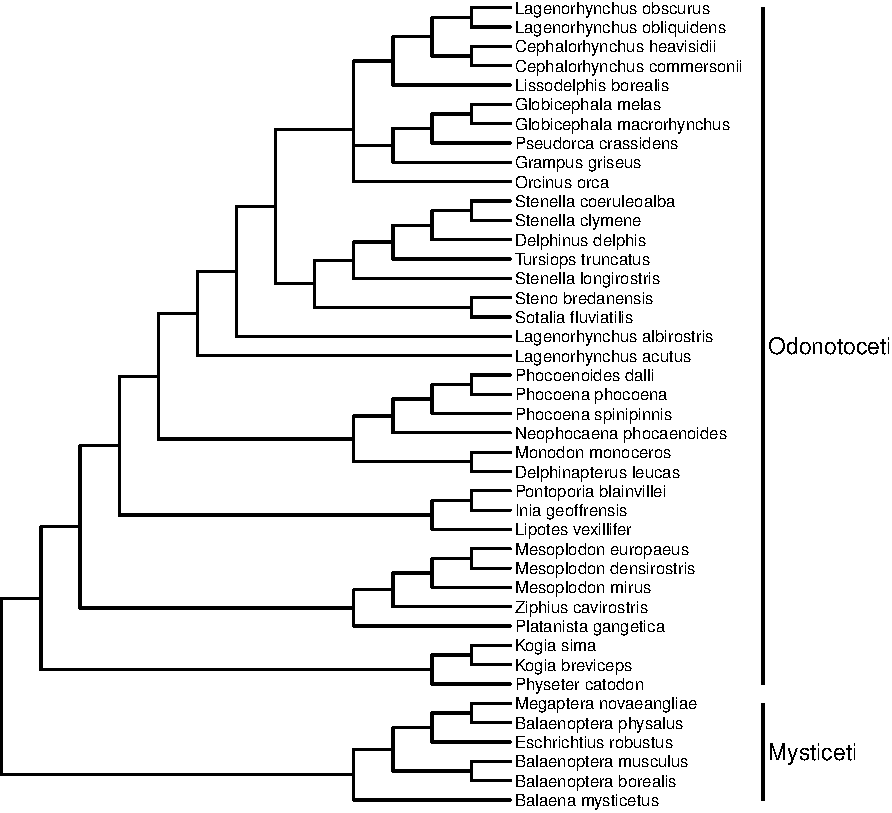
\includegraphics{bookdown-demo_files/figure-latex/unnamed-chunk-4-1} 

}

\caption{A cladogram of 42 cetacean species.}\label{fig:unnamed-chunk-4}
\end{figure}

The extant species are displayed on the \textbf{tips} of the tree and are connected to each other according to the degree of relatedness by the \textbf{branches}. Figure 2.1 shows us the pattern of relatedness of 42 cetacean species. If we wanted to use these species in a comparative study to investigate the evolutionary history of the group, we would not have independent data points. This means that the assumptions of most statistical tests would be violated and we couldn't trust the results!

This is where phylogenetics comes to the rescue. We can use the pattern of relatedness described by the phylogeny to control for the non-indepedence of data points. To show you what I mean, let's consider body size in those 42 species of cetacean. If we were to show the distribution of body size in the group, we would see that the vast majority of the largest sizes are found in the mysticetes whereas the smaller species tend to be odontocetes. If we viewed these data points as all independent we might say that very large bodies have evolved 7 times in the group (once for each mysticete and once for the sperm whale) whilst small body size has evolved in all the other species (35 times).

In fact, the close relatedness of 6 of the large bodied species suggests that large body size evolved once and not independently for each of these species. Their shared evolutionary history explains why their traits (body size in this case) are so similar. The seventh example of a large body (sperm whales) does not share very much history with the other 6 and this may be of some interest to us. It suggests an independent evolution of large body size and potentially something of interest to us as researchers.

So hopefully you can see how taking phylogeny into account can be illuminating. For a broader (and much more useful) introduction to phylogenetics and its use in evolutionary biology, check out these sources:

\begin{itemize}
\tightlist
\item
  Tree Thinking: An Introduction to Phylogenetic Biology \citep{baum12}
\item
  The Comparative Approach in Evolutionary Anthropology and Biology \citep{Nunn11}
\end{itemize}

\hypertarget{recap}{%
\chapter{R recap}\label{recap}}

In LIFE223, we taught you how to use R for statistical analysis and visualising data. This chapter will contain a basic overview of some of the things from 223 that you may find useful as we proceed. You only need to bother with this if you are new to R or have blocked it from your memory since you last used it.

\hypertarget{basics}{%
\section{Basics}\label{basics}}

R works well as a calculator.

\begin{Shaded}
\begin{Highlighting}[]
\DecValTok{6}\OperatorTok{*}\DecValTok{7}
\end{Highlighting}
\end{Shaded}

\begin{verbatim}
[1] 42
\end{verbatim}

However, R is capable of a great deal more than just simple mathematical operations like multiply and divide. It also has functions that can calculate some common descriptive stats like mean and standard deviation.

\begin{Shaded}
\begin{Highlighting}[]
\KeywordTok{mean}\NormalTok{(x)}
\end{Highlighting}
\end{Shaded}

\begin{verbatim}
[1] 41.99693
\end{verbatim}

\begin{Shaded}
\begin{Highlighting}[]
\KeywordTok{sd}\NormalTok{(x)}
\end{Highlighting}
\end{Shaded}

\begin{verbatim}
[1] 4.197835
\end{verbatim}

\hypertarget{plotting}{%
\subsection{Plotting}\label{plotting}}

R is also a very flexible graphical tool. From LIFE223, you probably remember a few basic plotting functions. Each function in R has arguments that can be added to label axes or change point size as you can see in these plots.

\begin{Shaded}
\begin{Highlighting}[]
\KeywordTok{boxplot}\NormalTok{(x, }\DataTypeTok{ylab =} \StringTok{"Potential answers"}\NormalTok{)}
\end{Highlighting}
\end{Shaded}

\begin{center}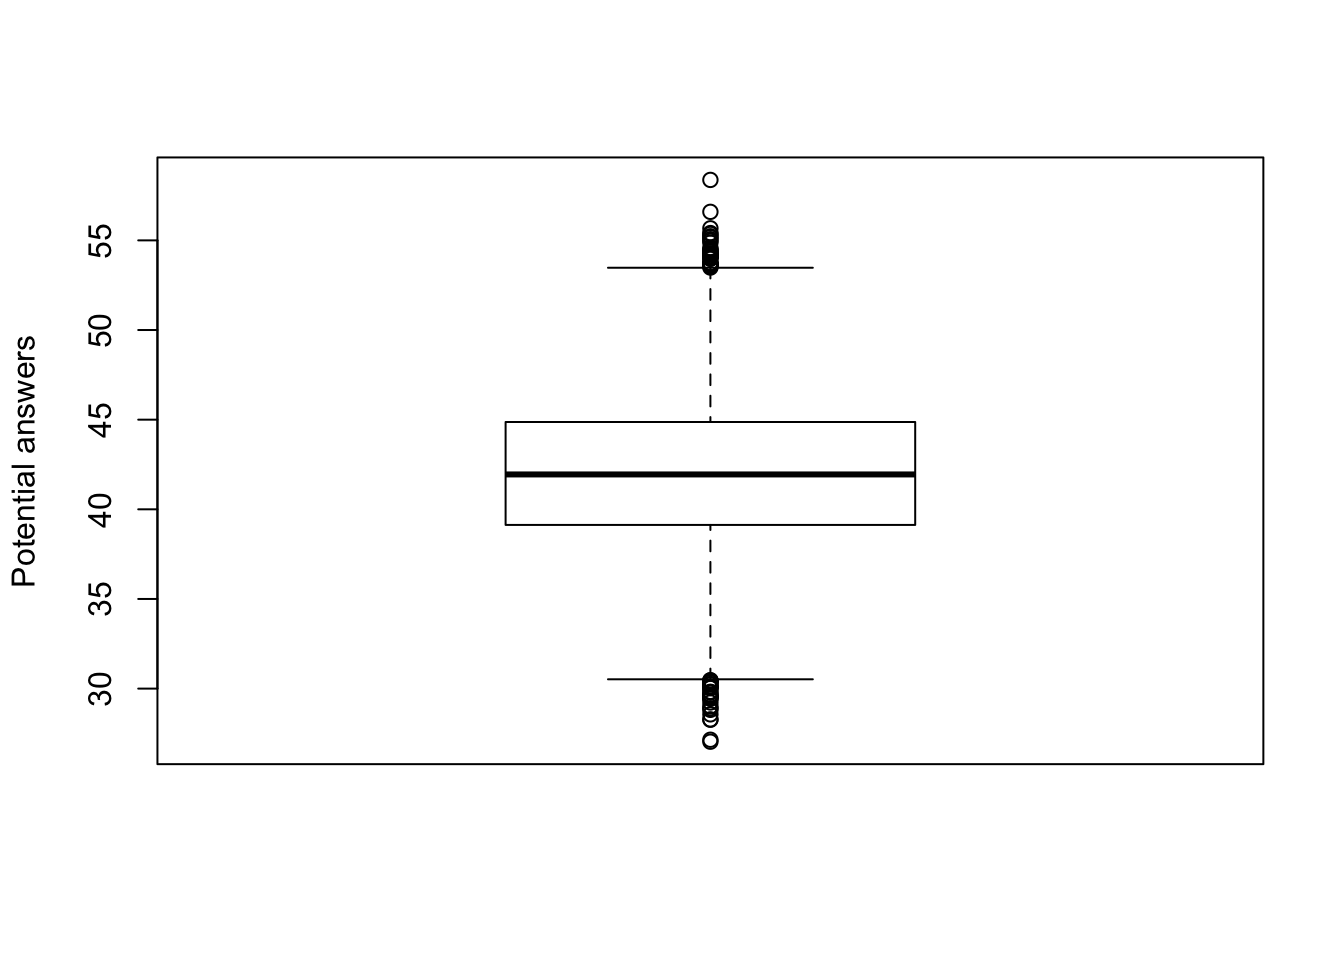
\includegraphics{bookdown-demo_files/figure-latex/unnamed-chunk-9-1} \end{center}

\begin{Shaded}
\begin{Highlighting}[]
\KeywordTok{hist}\NormalTok{(x, }\DataTypeTok{xlab =} \StringTok{"Potential answers"}\NormalTok{, }\DataTypeTok{breaks =} \DecValTok{25}\NormalTok{)}
\end{Highlighting}
\end{Shaded}

\begin{center}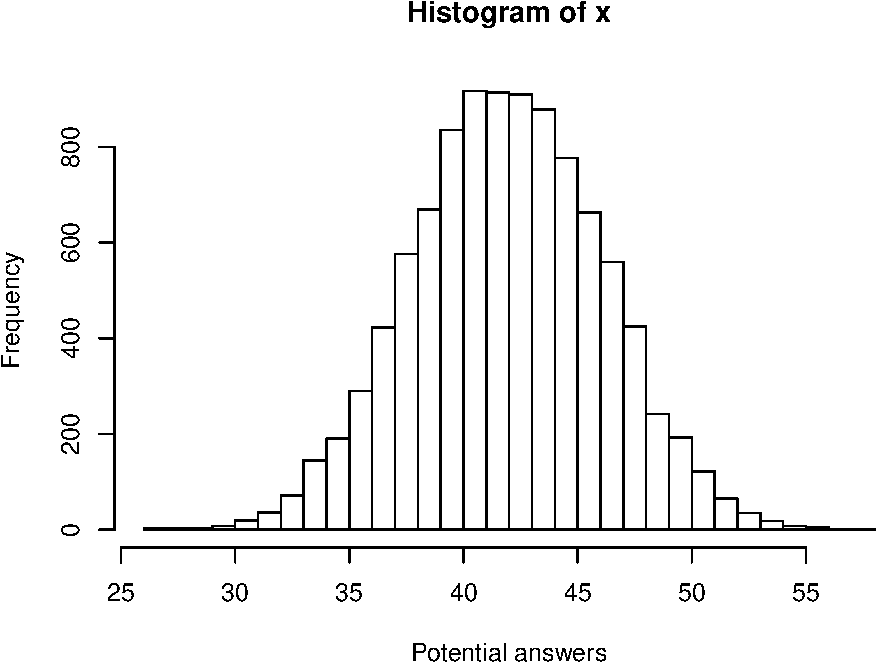
\includegraphics{bookdown-demo_files/figure-latex/unnamed-chunk-9-2} \end{center}

\begin{Shaded}
\begin{Highlighting}[]
\KeywordTok{plot}\NormalTok{(x, y, }\DataTypeTok{xlab =} \StringTok{"Potential answers"}\NormalTok{, }\DataTypeTok{pch =} \DecValTok{19}\NormalTok{, }\DataTypeTok{cex =} \FloatTok{0.1}\NormalTok{, }\DataTypeTok{ylab =} \StringTok{""}\NormalTok{)}
\end{Highlighting}
\end{Shaded}

\begin{center}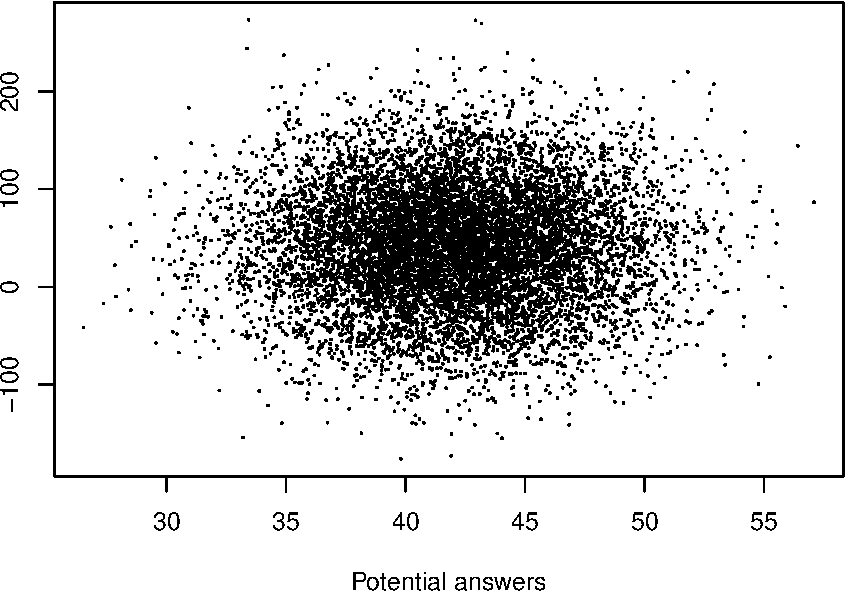
\includegraphics{bookdown-demo_files/figure-latex/unnamed-chunk-9-3} \end{center}

For much of this book, I will actually be doing most plotting in a package called \textbf{ggplot2} \citep{ggplot}. This package has a slightly different syntax to get used to but the increased flexibility you have will be a good payoff. Plus the plots look quite nice.

\begin{center}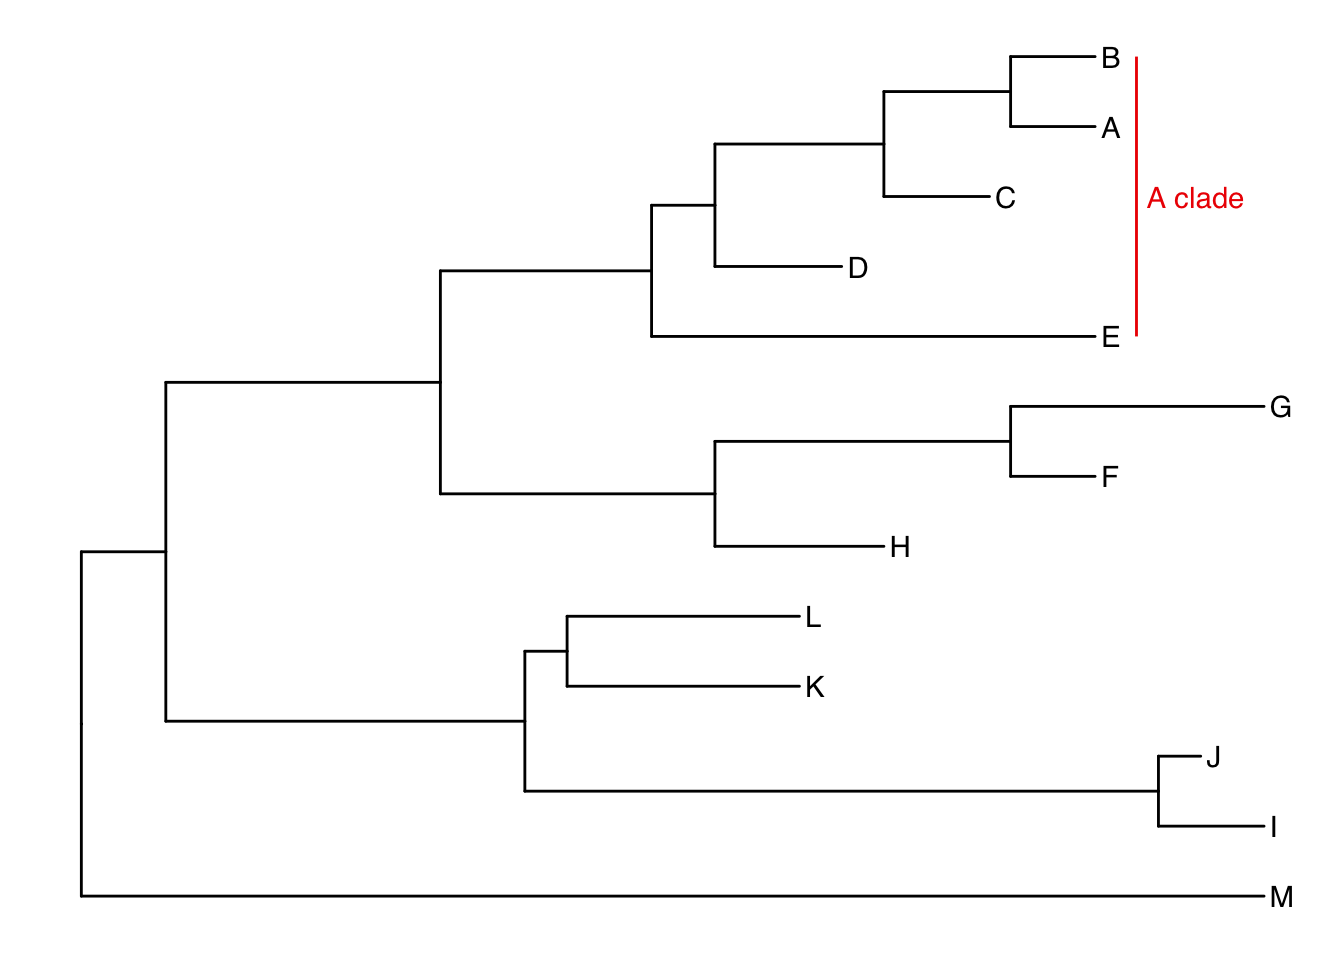
\includegraphics{bookdown-demo_files/figure-latex/unnamed-chunk-10-1} \end{center}

For all the details on how to use ggplot2, have a look at \href{https://ggplot2.tidyverse.org}{this bookdown} all about visualising data using ggplot2.

\hypertarget{the-working-directory}{%
\subsection{The working directory}\label{the-working-directory}}

The working directory is the folder on your computer where R's attention is focused. This is where you should store any files you need R to open. You can find out the path of the current working directory using the function \textbf{getwd()}

\begin{Shaded}
\begin{Highlighting}[]
\KeywordTok{getwd}\NormalTok{()}
\end{Highlighting}
\end{Shaded}

\begin{verbatim}
[1] "/Users/chrismitchell/Google Drive/University of Liverpool/GitHub Stuff/bookdownCRG"
\end{verbatim}

If this isn't the folder we want as our working directory, we can just as easily change it with \textbf{setwd()}

\begin{Shaded}
\begin{Highlighting}[]
\KeywordTok{setwd}\NormalTok{(}\StringTok{"\textasciitilde{}/Desktop/My R Folder"}\NormalTok{)}
\end{Highlighting}
\end{Shaded}

If you are using RStudio there is also a shortcut to do this in the \textbf{Files} pane (usually bottom right). Use this pane to navigate to your chosen directory and then use the drop down menu under \textbf{More} (look for a blue cog) to set the current folder as your working directory.

If you aren't using RStudio, I'd strongly suggest you start. It's much more user friendly than base R.

\hypertarget{loading-data}{%
\subsection{Loading data}\label{loading-data}}

Data comes in many forms and R is capable of reading most of them if you know the correct functions. One of the most common formats is \emph{comma separated values}. This has the file extension .csv at the end of the filename. If you open a .csv file with MS Excel or Numbers, you will see that it usually looks much like a spreadsheet. To load a .csv data file into R, use the function \textbf{read.csv()} as shown here.

\begin{Shaded}
\begin{Highlighting}[]
\NormalTok{data \textless{}{-}}\StringTok{ }\KeywordTok{read.csv}\NormalTok{(}\DataTypeTok{file =} \StringTok{"DATAFILE.csv"}\NormalTok{)}
\end{Highlighting}
\end{Shaded}

For other data formats, you may require a different function. For example, data may be provided as a text file (extension .txt). In this case, you need \textbf{read.table()}. Note that with this function you need to specify that your data has a header (a top row with names for columns) whereas \textbf{read.csv()} assumes this by default.

\begin{Shaded}
\begin{Highlighting}[]
\NormalTok{data \textless{}{-}}\StringTok{ }\KeywordTok{read.table}\NormalTok{(}\DataTypeTok{file =} \StringTok{"DATAFILE.txt"}\NormalTok{, }\DataTypeTok{header =} \OtherTok{TRUE}\NormalTok{)}
\end{Highlighting}
\end{Shaded}

\hypertarget{subsetting}{%
\subsection{Subsetting}\label{subsetting}}

Let's say I want to subset my data based on a certain condition. I can achieve this multiple ways but one of the simplest is the function \textbf{subset}.

\begin{Shaded}
\begin{Highlighting}[]
\NormalTok{newdata \textless{}{-}}\StringTok{ }\KeywordTok{subset}\NormalTok{(data, species }\OperatorTok{==}\StringTok{ "Homo sapiens"}\NormalTok{)}
\end{Highlighting}
\end{Shaded}

This function takes a subset of the object \textbf{data} and applies the rule that the value of each row in the column \emph{species} be \emph{Homo sapiens}. Thus it extracts the lines of data that are from human beings.

\hypertarget{errors}{%
\section{Errors}\label{errors}}

Error messages are a part of life with R. You are not expected to be able to interpret every single one immediately and you definitely shouldn't panic or give up when you get one.

Here's a basic error message:

\begin{Shaded}
\begin{Highlighting}[]
\NormalTok{data \textless{}{-}}\StringTok{ }\KeywordTok{read.csv}\NormalTok{(}\StringTok{"mydaat.csv"}\NormalTok{)}
\end{Highlighting}
\end{Shaded}

\begin{verbatim}
Warning in file(file, "rt"): cannot open file 'mydaat.csv': No such file or
directory
\end{verbatim}

\begin{verbatim}
Error in file(file, "rt"): cannot open the connection
\end{verbatim}

The message tells me that R ``cannot open the connection'' and no such file exists. This means that R cannot find the file I was looking for in the current working directory. It could be because I haven't set the correct working directory or the file is there but in a different format. In this case, the error has appeared because I have spelled the name incorrectly. I have sent R looking for a file called \emph{mydaat.csv} instead of \emph{mydata.csv}. Always remember that R is a useful idiot and will only do exactly what you tell it to do!

\hypertarget{google}{%
\section{Google}\label{google}}

The most important skill you need for using R is the ability to use Google (other search engines are available). It may seem odd but almost any problem you will ever encounter with R can be solved by a quick Google search.

If you come up against a confusing error message, copy and paste the message into Google. You will quickly land on one of the forums where someone else has asked about the same error message. The odds are pretty good you'll discover an explanation for the problem there.

If you don't know how to do something, pop the name of what you want to do into Google and add ``in R'' at the end and there will almost always be a tutorial on the first page of results with exactly what you need.

Seriously, Google is your strongest ally here. The community of R users has populated the internet with endless advice and guidance for every level from beginner to the most advanced of users. That brings me to my next point\ldots{}

\hypertarget{stealing}{%
\section{Stealing}\label{stealing}}

If imitation is the greatest form of flattery then learning to code in R is just about the most flattering thing you can do. The internet is teeming with examples of R code for all kinds of purposes including in this very book. Take it without thinking twice.

You will have acheived a pretty good level of skill in R when you can take someone else's code and edit it for your own purposes. This is the \textbf{core skill} of R and once you can do that, you'll be unstoppable.

\hypertarget{phylogenetics}{%
\chapter{Phylogenetic trees and where to find them}\label{phylogenetics}}

This chapter is a brief overview of some key concepts that may be useful when performing comparative research.

\hypertarget{phylogeny}{%
\section{Phylogeny}\label{phylogeny}}

Phylogeny is the term used to describe the evolutionary history of a group of species. The most common representation of phylogeny is a phylogenetic tree. There is a lot of terminology around phylogenetic trees. Here we will start with the very basics that will come up a lot in this book.

The \textbf{tips} of the tree represent the species/populations/individuals described by the tree. The \textbf{branches} of the tree represent the pattern of relationships between species. The \textbf{nodes} of a tree represent the most recent common ancestor of the lineages that diverge from that node. A \textbf{clade} is a monophyletic grouping of lineages. A grouping is \textbf{monophyletic} only if all members of that group descend from a common ancestor to the exclusion of others. For example, humans and apes form a monophyletic grouping but humans, apes and parrots do not.

Here is an example of a phylogenetic tree displaying the relationships of modern dog breeds taken from a nice paper investigating the evolutionary history of the domestic dog \citep{Parker17}

\begin{figure}[H]

{\centering 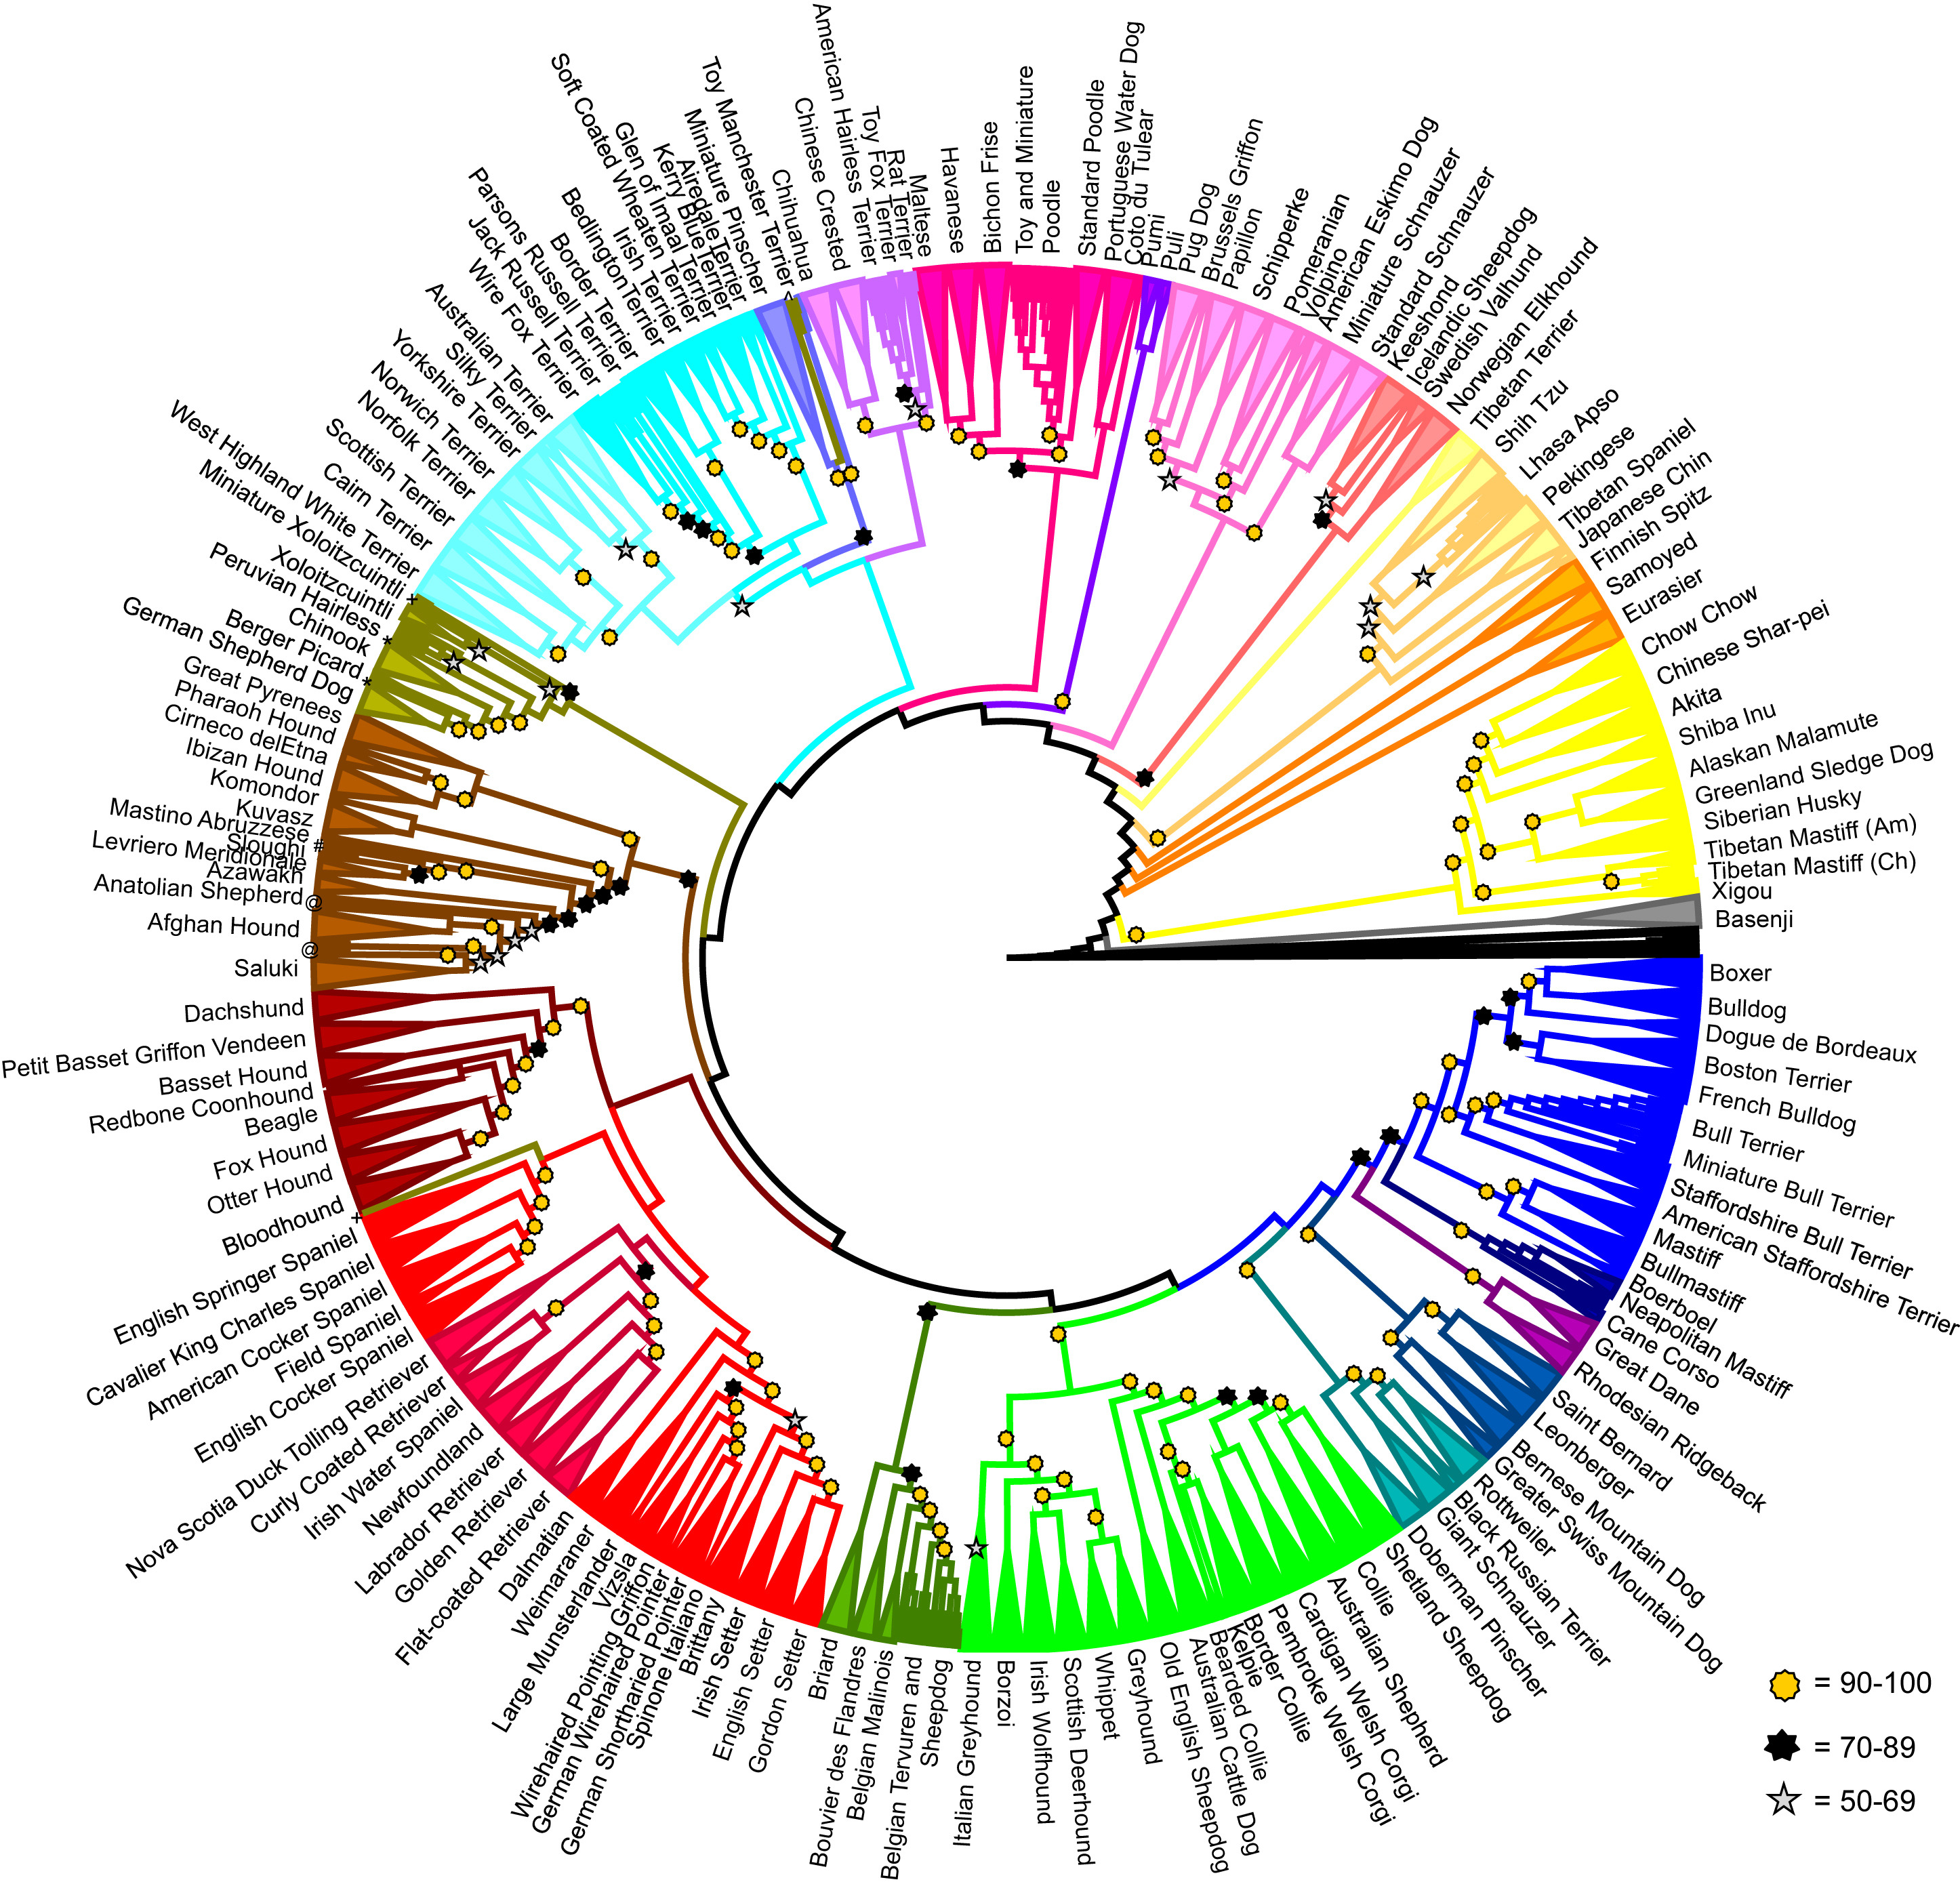
\includegraphics[width=40.17in]{Images/dogs} 

}

\caption{Cladogram of 161 domestic dog breeds taken from Parker et al 2017.}\label{fig:unnamed-chunk-18}
\end{figure}

The tree shown above is a \textbf{cladogram} meaning that the lengths of the branches do not carry any real meaning. This tree is only useful for interpreting the relatedness of the species. It does not give us any information about the amount of evolutionary change or the amount time between nodes.

By contrast, the following tree has \textbf{branch lengths}. The tree is based on genetic analysis of 173 species of hymenoptera (bees, ants and wasps) \citep{Peters17}. In this tree, the branch lengths represent time (in millions of years) as calculated from analysis of over 3,000 genes and calibrated using fossils.

\begin{figure}[H]

{\centering 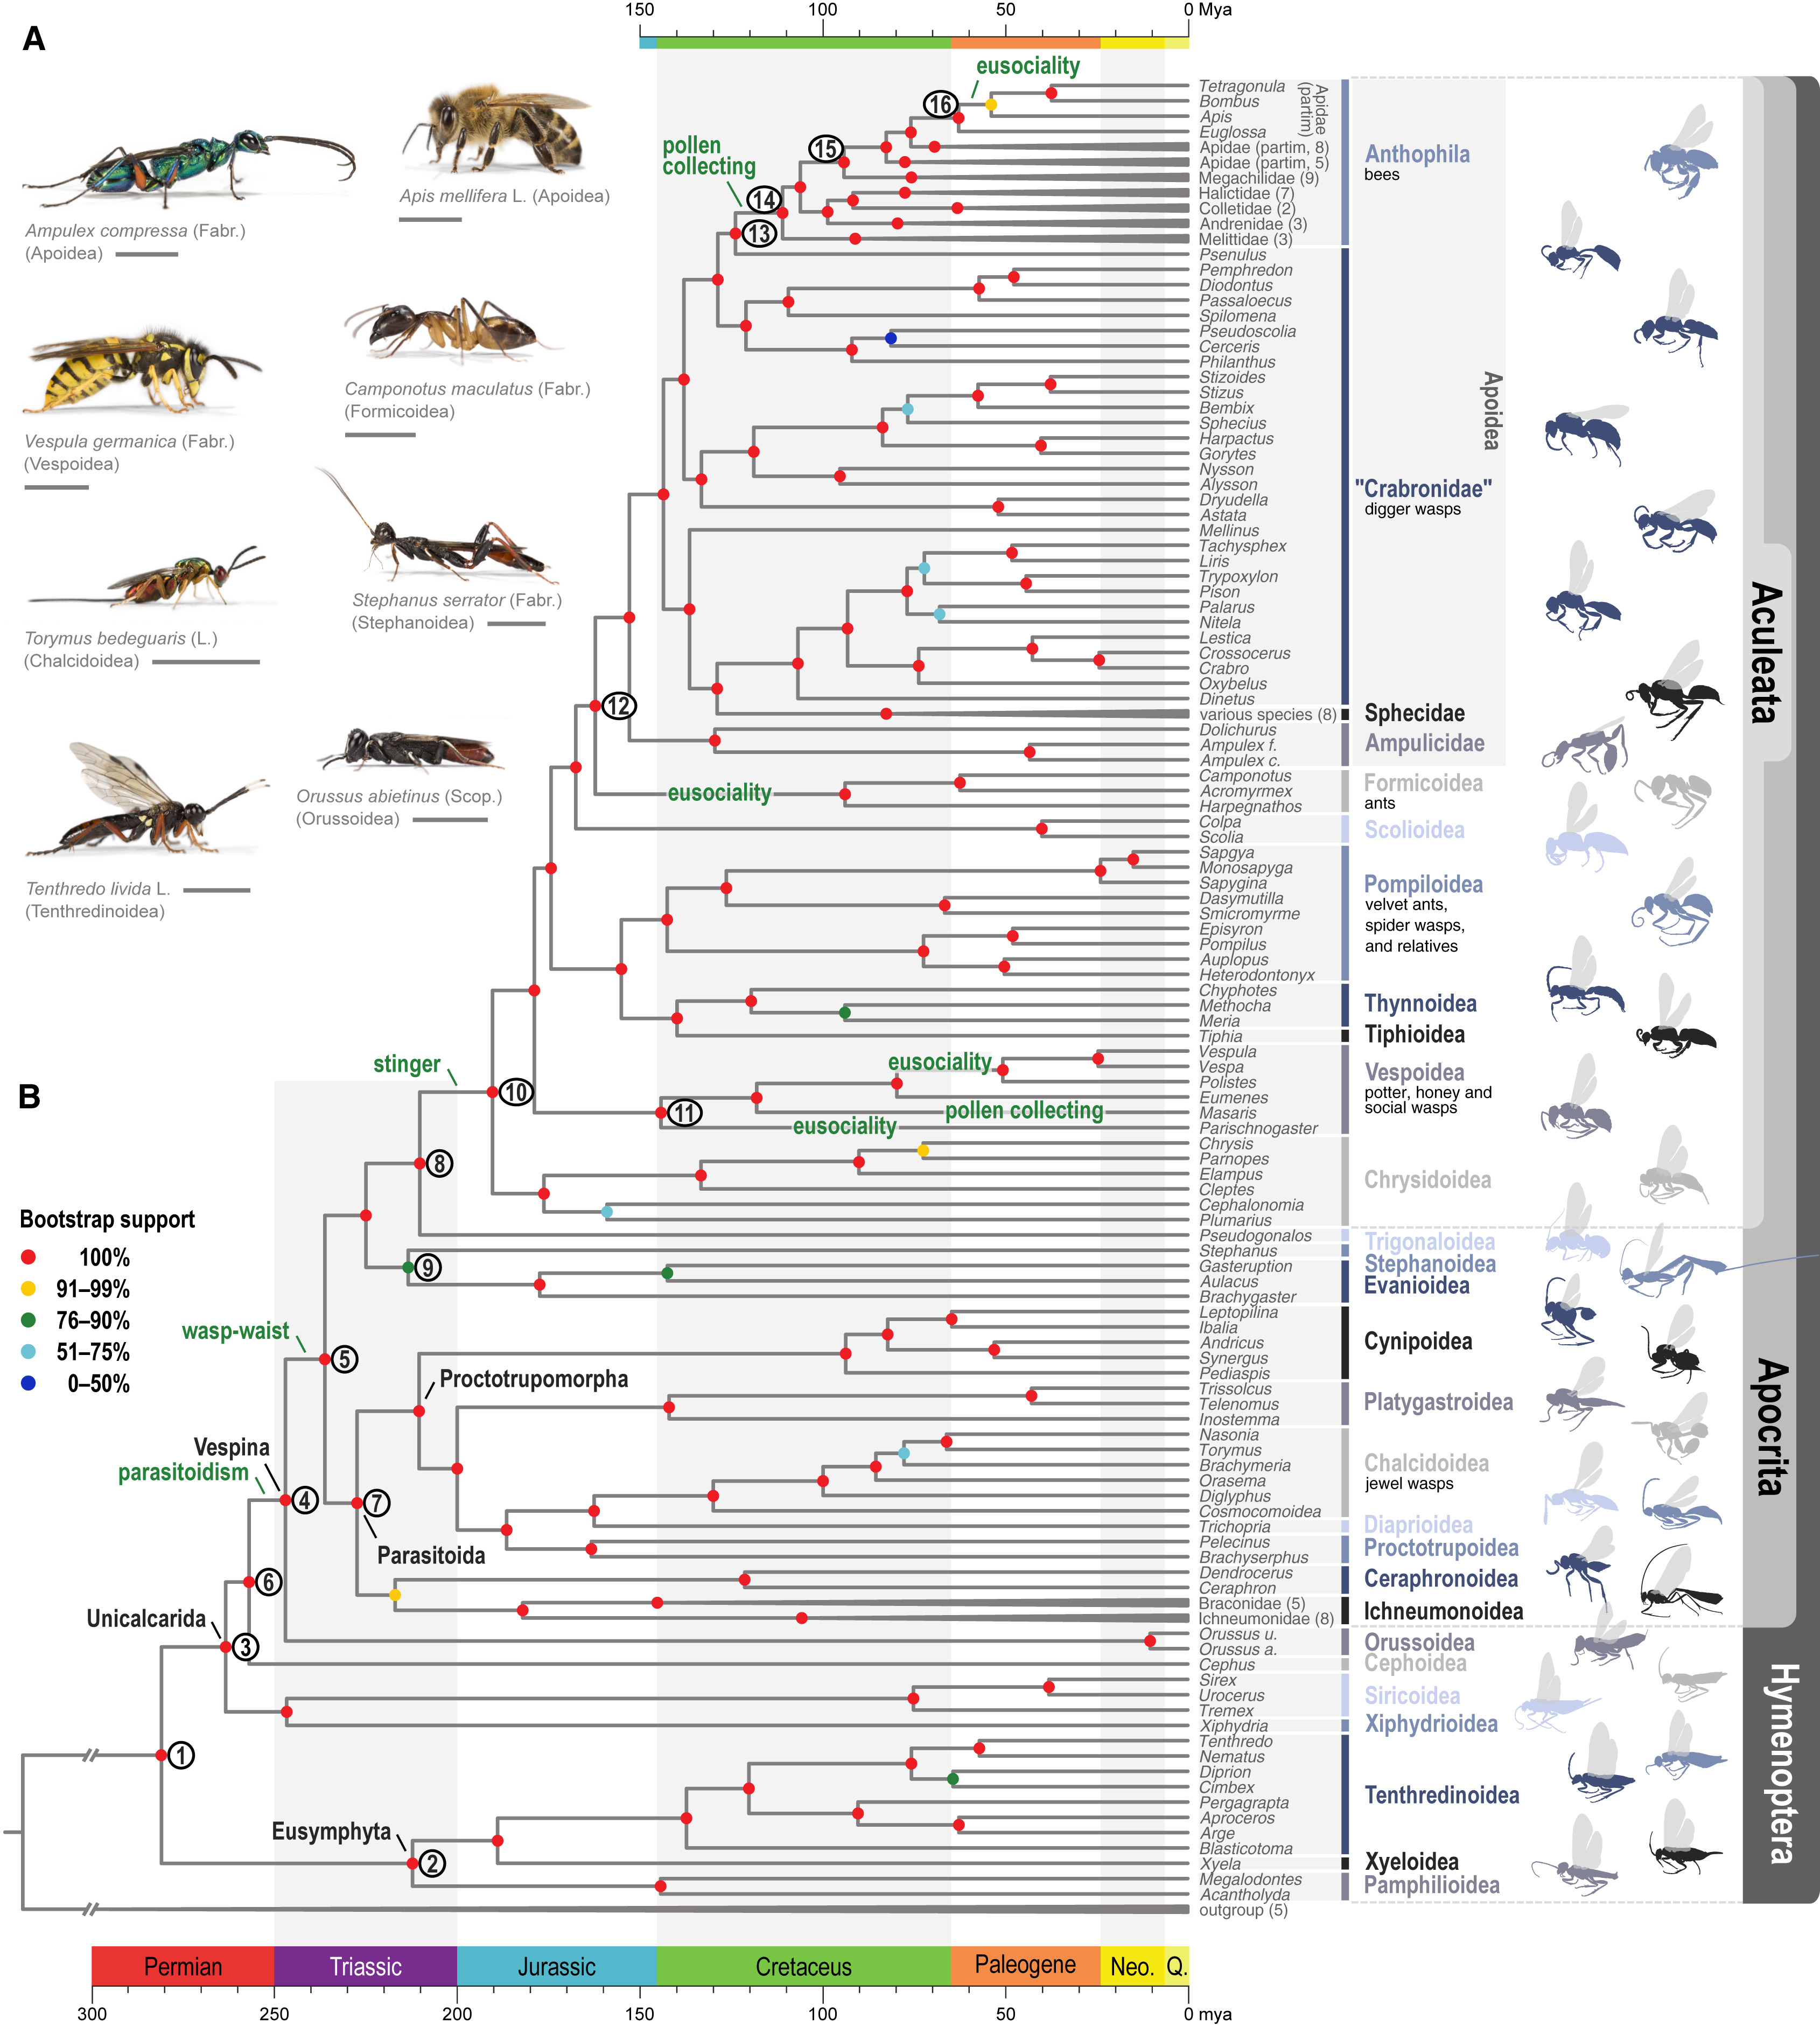
\includegraphics[width=46.94in]{Images/hymenoptera} 

}

\caption{Time-calibrated phylogeny of Hymenoptera from Peters et al 2018.}\label{fig:unnamed-chunk-19}
\end{figure}

Branch lengths do not always represent evolutionary distance as time. In some cases, evolutionary distance is represented as the amount of change on each branch. The next tree was built based on a brain development gene (MCPH1) in cetaceans (whales, dolphins and porpoises) \citep{McGowen11}. On a tree like this, longer branches indicate more character changes along the branch. In this case the character changes will be changes in genetic sequence but for other trees it may be morphological characters, protein sequences or a combination of molecular and morphological traits.

\begin{figure}[H]

{\centering 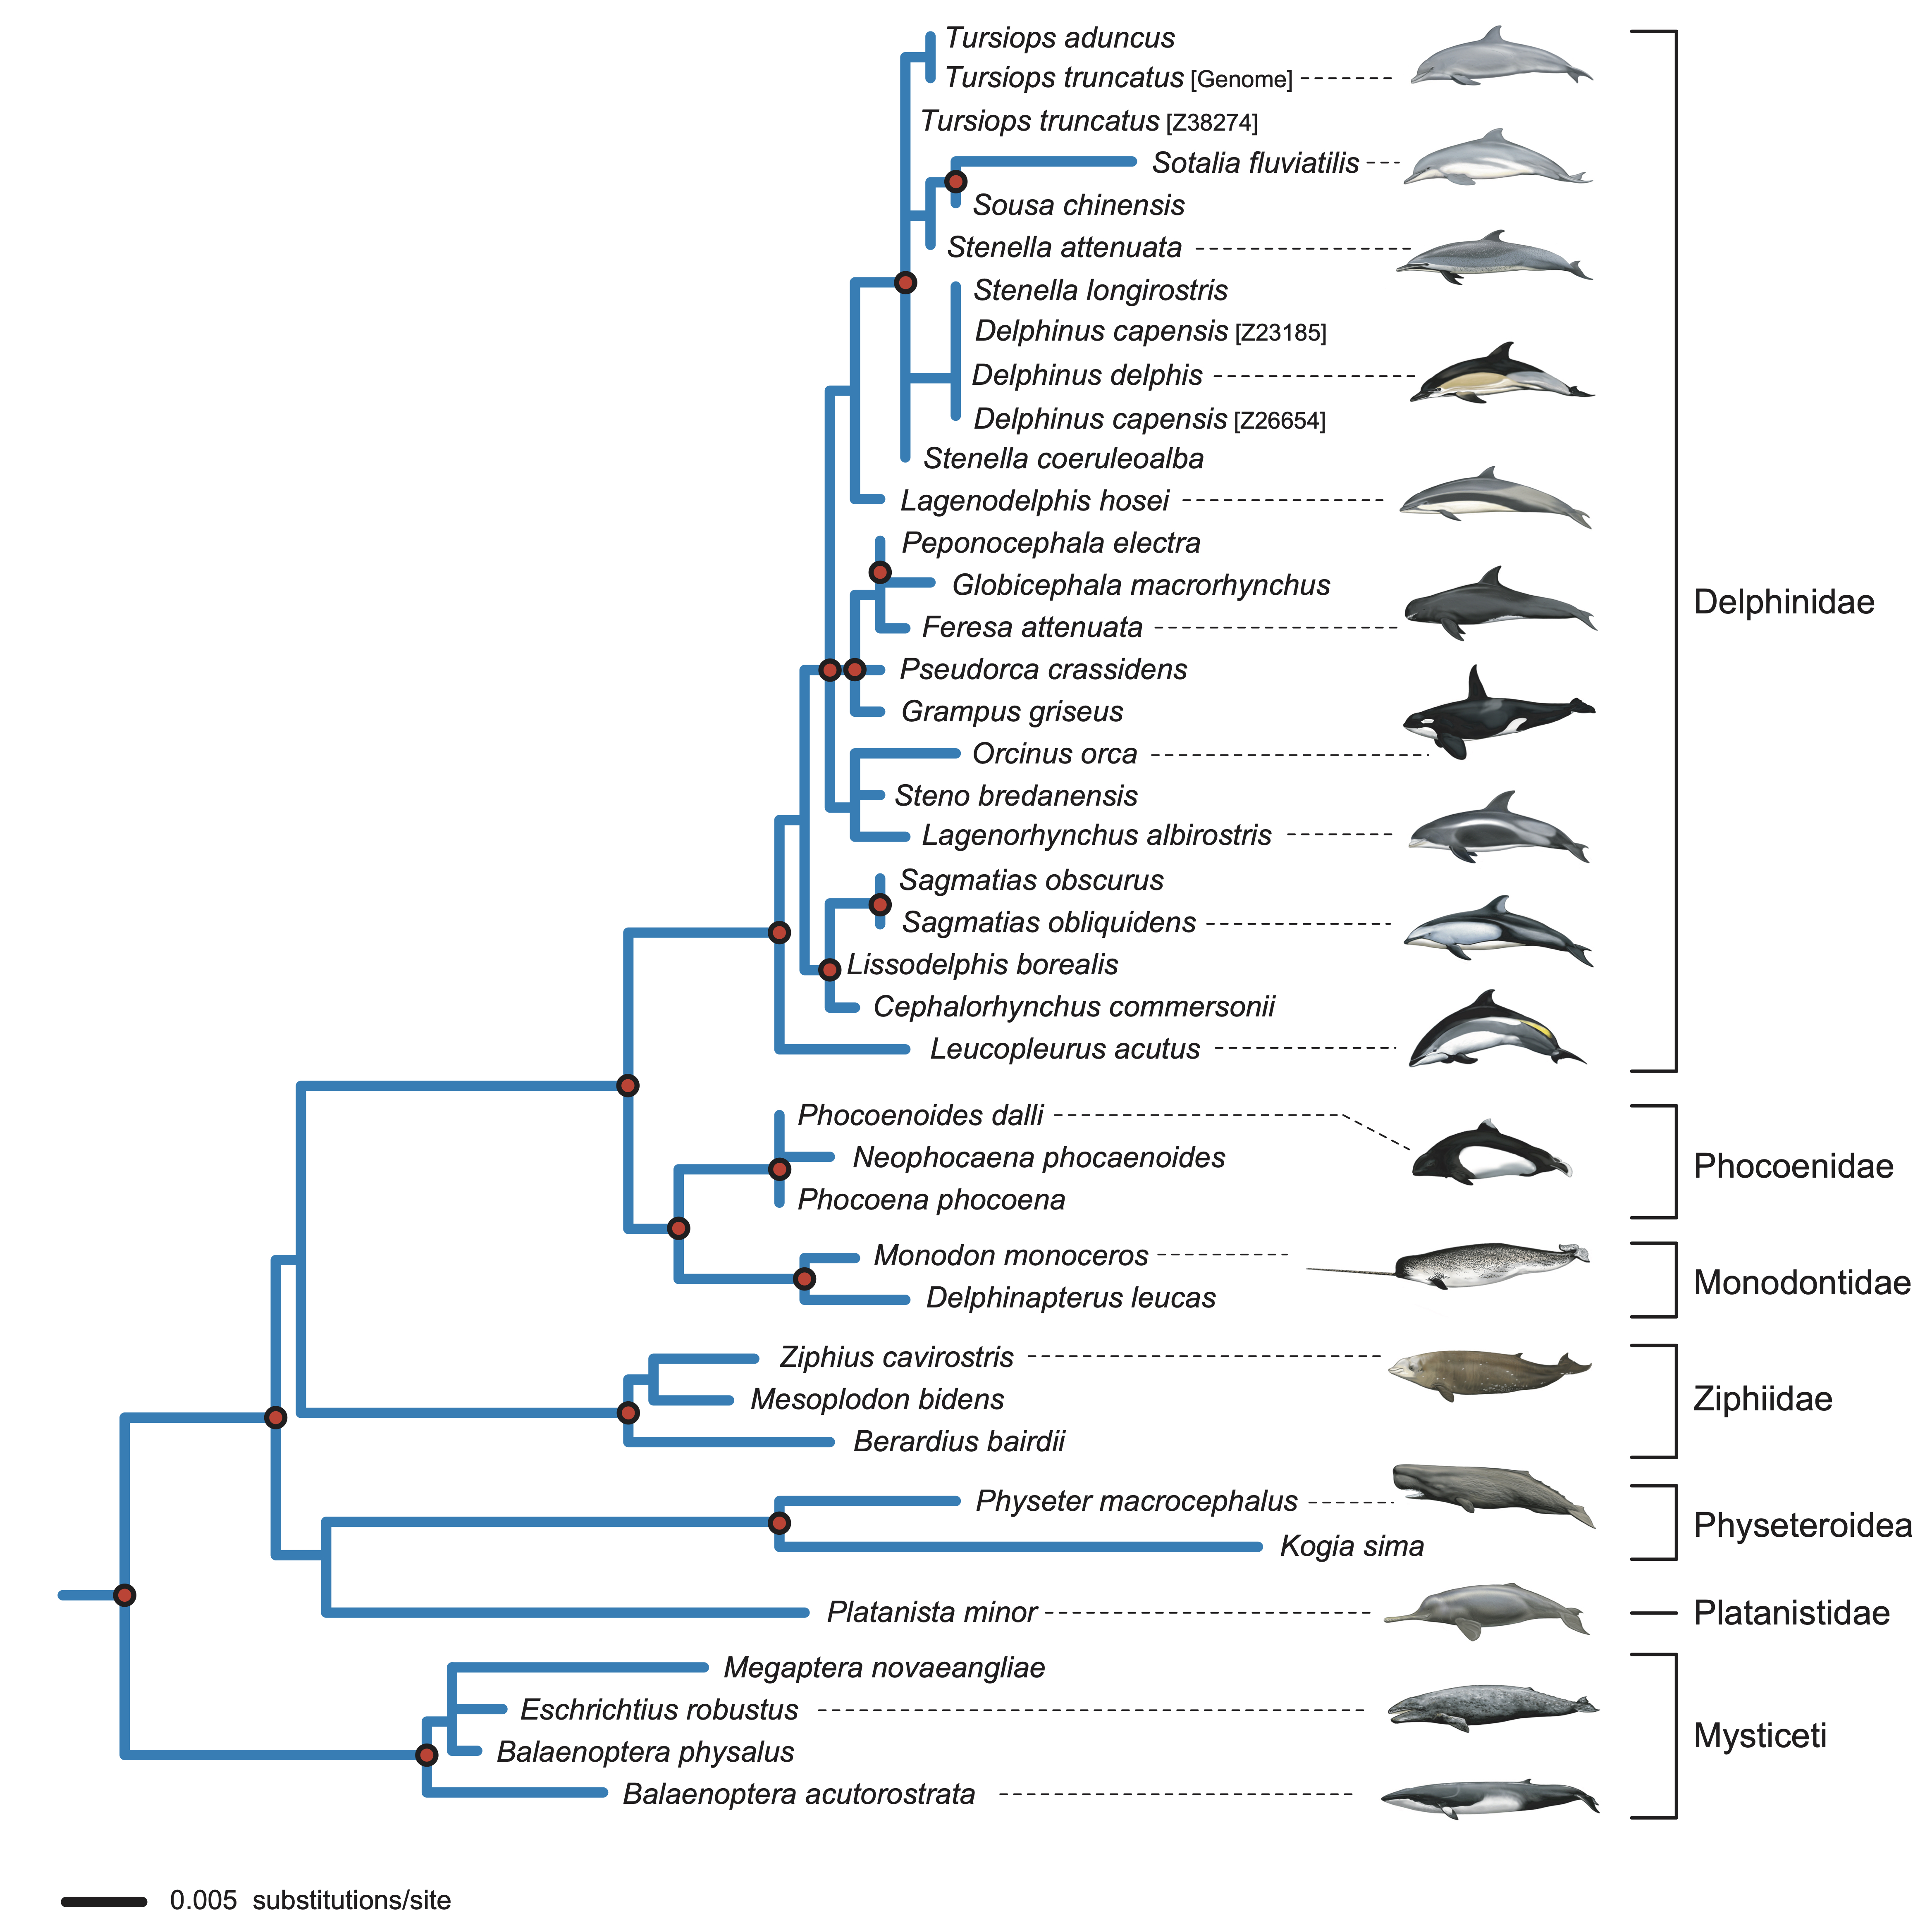
\includegraphics[width=64.9in]{Images/whales} 

}

\caption{Phylogeny of MCPH1 brain development gene in 38 cetacean species from McGowen et al 2011.}\label{fig:unnamed-chunk-20}
\end{figure}

\hypertarget{building-trees}{%
\section{Building trees}\label{building-trees}}

Developments in the field of phylogenetics have meant that there are many ways to construct a phylogeny. Many of the modern methods are highly sophistaicated and for now, these are not the subject of this book. However, it may help you to have a brief introduction to the logic behind building a phylogeny.

For three species, there are only 3 possible phylogenies.

\begin{center}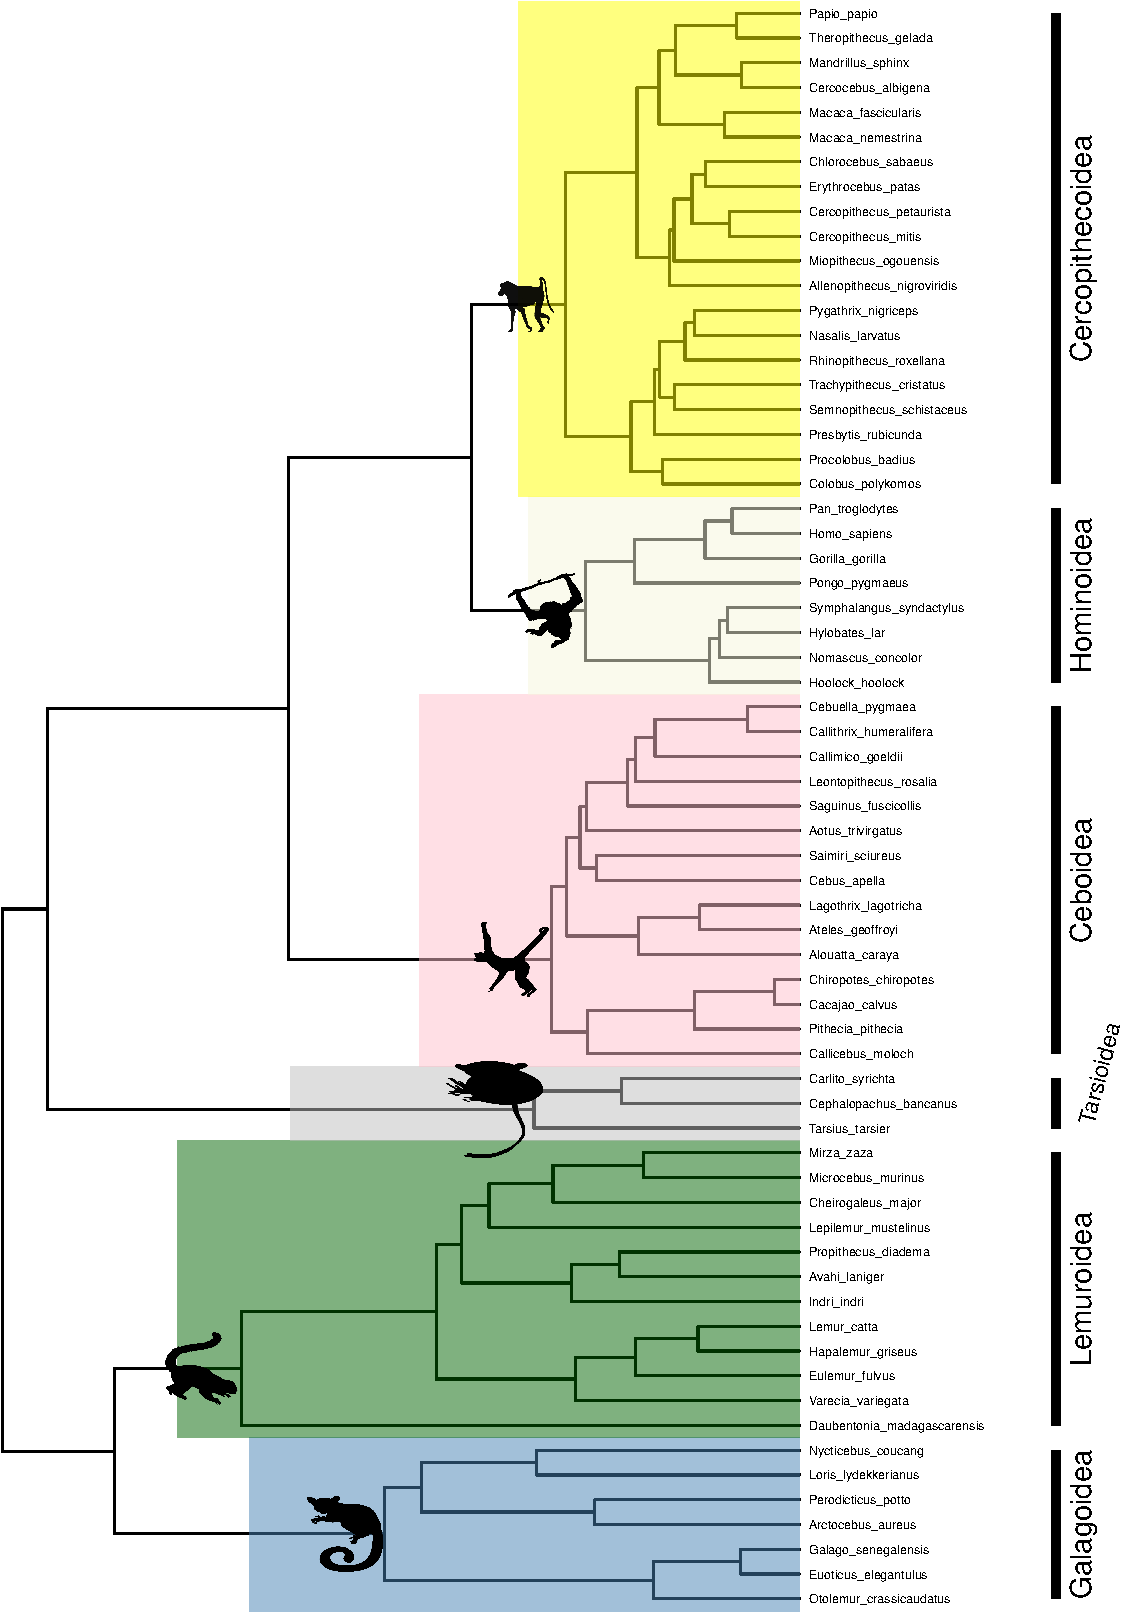
\includegraphics{bookdown-demo_files/figure-latex/unnamed-chunk-21-1} \end{center}

For 5 species, there are 105 possible phylogenies. For 10 species, there are 34.5 million possible trees! Clearly we need a great deal of computational power to distinguish between all these possibilities.

To understand the scale of this problem, it may be useful to contemplate the tale of \emph{The Maharaja's Rice}, a legend in Hindu fokelore. The legend goes that a local king would challenge visitors to a game of chess. Such was the confidence of the king that if the visitor defeated him, they could name their reward. One day, a humble traveller accepted the challenge and named a few grains of rice as his reward. If he won, the king would have to place one grain on the first square of the board, 2 on the second square, 4 and third and so on, doubling the number for each square.

Delighted by the apparently low stakes, the king accepted but to his dismay, lost the game. Humbled by defeat, he called for a sack of rice to settle the debt. As he began laying out the grains, he realised that the traveller had tricked him.

\begin{center}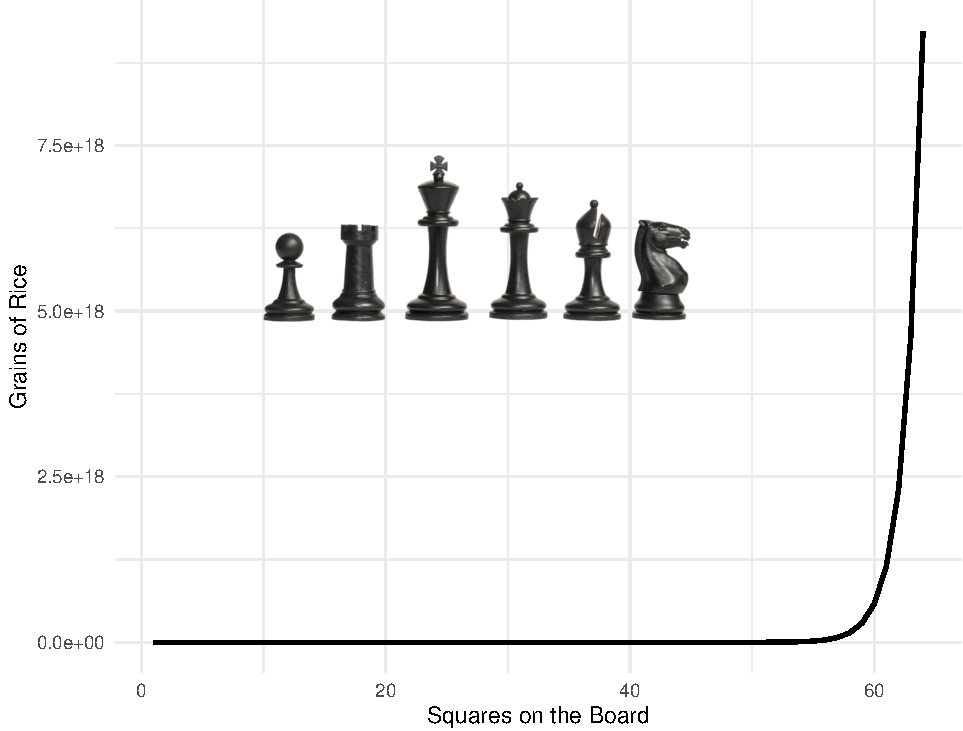
\includegraphics{bookdown-demo_files/figure-latex/unnamed-chunk-22-1} \end{center}

The amount of rice grew exponentially. On the \(\text{32}^{\text{nd}}\) square, there were 2 billion grains of rice. On the \(\text{64}^{\text{th}}\) and final square alone, there would be \(1.8 \times 10^{19}\) grains which equates to over 200 billion tons of rice. The traveller revealed himself as Krishna and allowed the king to repay the debt over time. To the present day, people visiting the area are served Paal Paysam to repay the debt to Krishna.

The point here is that we are generally very poor at considering very large numbers and when we are dealing with phylogenetics, it is a good idea to bear this in mind. Consider the vast number of possible relationships there are between the almost 6,000 species of mammal!

Obviously we need to narrow down the possibilities to something more reasonable. The process of building a tree is always the same. Compare a number of traits across a group of species and determine the points of similarity and difference. The more similar two species are, the more closely related they will be in the resulting phylogeny. Let's have a look at how this works with different traits

\hypertarget{morphology}{%
\subsection{Morphology}\label{morphology}}

Classically, species were sorted into groupings based on morphological similarity. For example, the following table is a character matrix for 5 traits across 6 species. The presence of a character is indicated by 1 and the absence by 0.

\begin{tabular}{l|c|c|c|c|c|c}
\hline
  & Lancelet & Lamprey & Bass & Frog & Turtle & Leopard\\
\hline
Backbone & 0 & 1 & 1 & 1 & 1 & 1\\
\hline
Hinged Jaw & 0 & 0 & 1 & 1 & 1 & 1\\
\hline
4 Limbs & 0 & 0 & 0 & 1 & 1 & 1\\
\hline
Amnion & 0 & 0 & 0 & 0 & 1 & 1\\
\hline
Hair & 0 & 0 & 0 & 0 & 0 & 1\\
\hline
\end{tabular}

We can use this matrix to construct a cladogram. Evidently the turtle and leopard have the most in common (4 out of 5 traits) and then the frog has 3 traits in common with both of them. In this way, we can build our tree.

\begin{center}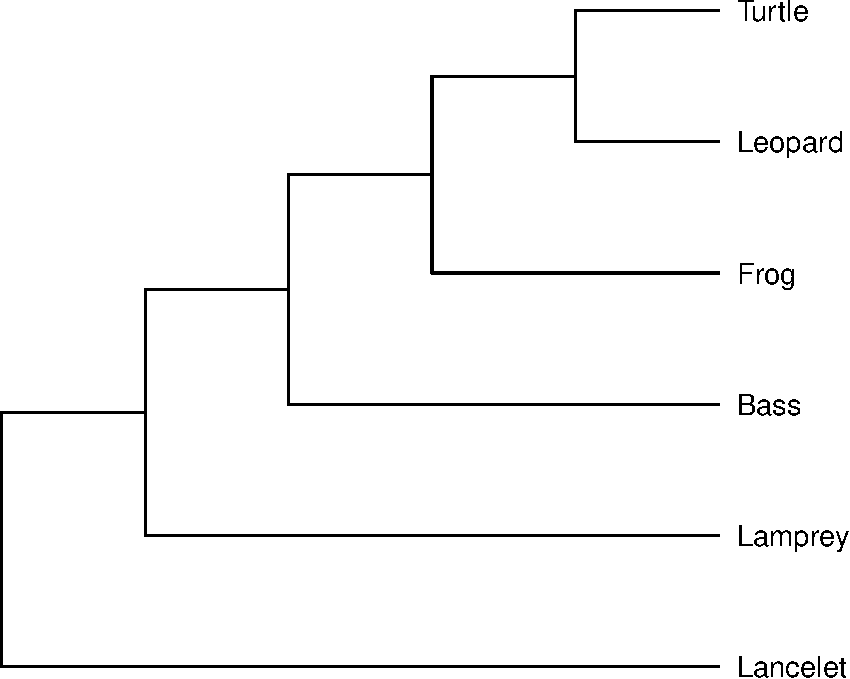
\includegraphics{bookdown-demo_files/figure-latex/unnamed-chunk-24-1} \end{center}

Using morphological similarity is simple enough because the traits are mostly easily observable. However, we need to be careful. The choice of trait is vitally important here. For example, we may be in danger of mistaking homologous traits and analogous traits. Flight adaptations in birds, bats, pterosaurs and insects represent examples of distantly related animals converging on similar triats and certainly not common descent.

Let's take the example of cetaceans (whales, dolphins and porpoises). Historically, some had thought cetaceans were large fish with sources as late as the \(\text{17}^{\text{th}}\) century CE referring to porpoises as fish. This is despite ancient sources such as Aristotle who noted their remarkable similarity to terrestrial vertebrates in the \(\text{4}^{\text{th}}\) century BCE. By the \(\text{18}^{\text{th}}\) century CE, cetaceans were formally recognised as mammals but even then, it was clear that were very different.

So how should we classify them? A nice common sense grouping might be alongside the other aquatic mammals. This would create a marine mammal clade of cetaceans, pinnipeds (seals \& sea lions) and the sirenians (manatees \& dugong). We might even place partially aquatic species like polar bears and otters as an outgroup to this clade.

The problem here is that \emph{living in the water} is not really a phylogenetically informative trait. It's the same trap people fell into when they classified whales as fish. What we need is to select traits that are phylogenetically informative, meaning that similarity in such traits is likely to reflect homology rather than analogy.

Often, tooth and jaw morphology are prominent in phylogenetics. These are hard-wearing parts of the skeleton that fossilise easily and since they are involved in feeding, they can tell you a lot about the animal. This makes them good sources of information when we can find them. Cladistic analyses based on morphological characteristics placed cetaceans as the sister group to a carnivorous group of extinct mammals called the mesonychids.

This intially made sense as cetaceans are carnivorous and this agreed with Darwin's 1859 postulation that cetaceans could have arisen from some form of swimming bear which gradually became more and more adapted to marine life. Upon closer inspection, mesonychids were found to have morphological similarities to artiodactyls (even-toed ungulates) and the clade was moved from carnivora to be a sister group of the artiodactyls.

\begin{center}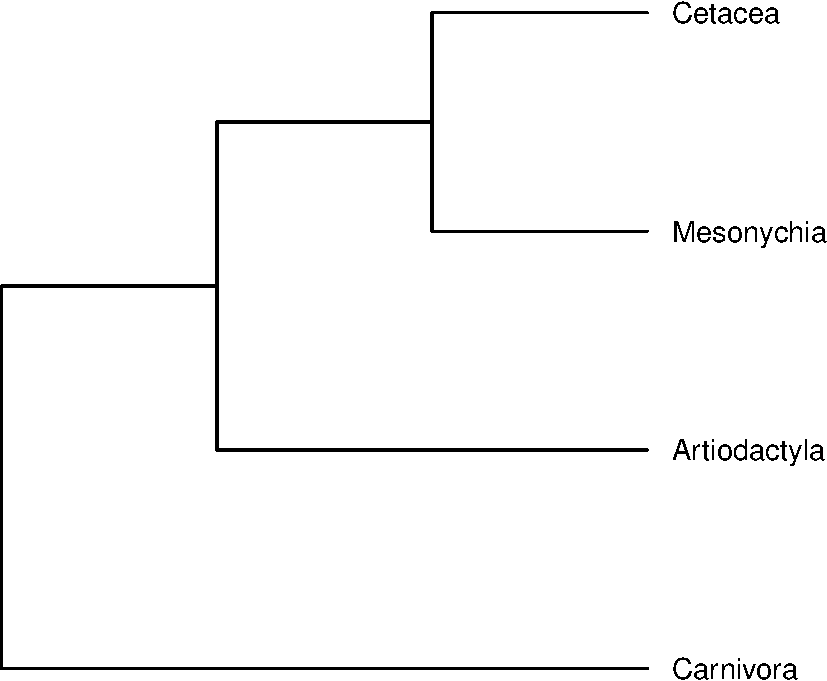
\includegraphics{bookdown-demo_files/figure-latex/unnamed-chunk-25-1} \end{center}

\hypertarget{molecular-data}{%
\subsection{Molecular data}\label{molecular-data}}

The relationship of cetaceans was all settled and agreed upon until somebody looked at the molecular data. As you know, all life is connected by DNA and over recent decades, it has become possible to sequence that DNA. This opened up new possibilities for traits to use in phylogenetics.

Molecular traits can be used just like morphological traits. So in the same way we look for similarities in tooth morphology, we can now look for similarities in DNA sequence and protein structure (amino acid sequence) as well. For the cetaceans, molecular analysis showed remarkable similarity between cetaceans and artiodactyls, suggesting that the two groups were monophyletic. The two groups are so closely related genetically, that the orders were combined to give us the presently accepted Cetartiodactyla.

\begin{center}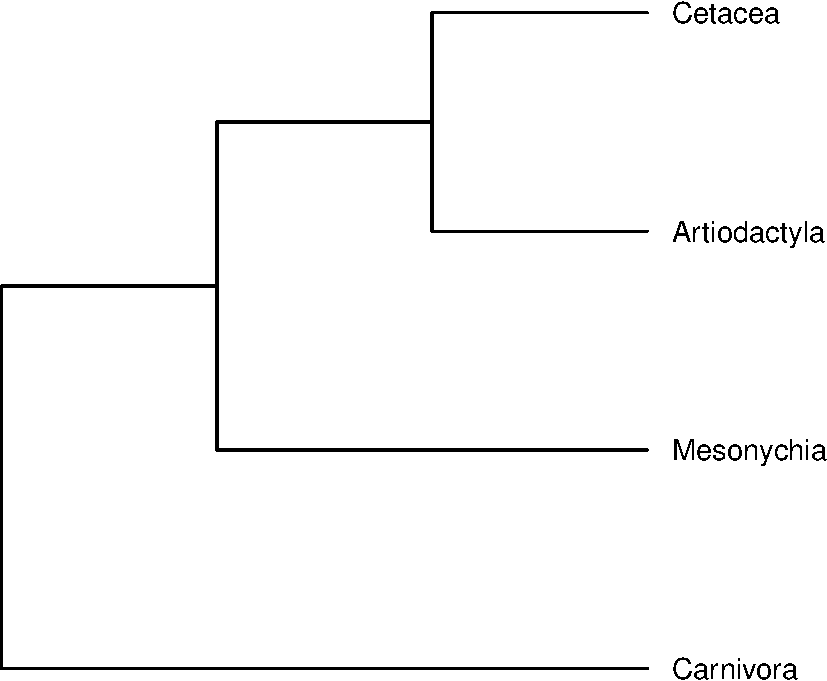
\includegraphics{bookdown-demo_files/figure-latex/unnamed-chunk-26-1} \end{center}

Modern phylogenies are built based on large matrices of characters. Often, morphological and molecular characters are used together to resolve phylogenies.

\hypertarget{tree-structure}{%
\section{Tree structure}\label{tree-structure}}

Phylogenetic trees are quite broadly available for researchers to use in comparative studies. The coverage of your study lineage will vary depending on how well studied the group is. This section will cover the basics of how phylogenies are represented by computers before pointing you to some of the places you will find trees to use.

To represent a phylogenetic tree we use \textbf{Newick format} which consists of nested brackets describing the relationships between pairs of species. Below is an example of a simple 3 species tree in which the two species of echidna are sister taxa and the platypus is the outgroup. Note the placement of the brackets (each pair of brackets wraps around sister taxa). The semicolon at the end is important to signify the end of the text string as well.

\[ ((\text{Short-beaked echidna , Long-beaked echidna})\text{, Platypus}); \]

We can manually write our own tree by passing this exact text string directly to the function \textbf{read.tree} in the package \textbf{ape} \citep{ape}. When we plot it, you'll notice that it is a cladogram because we haven't supplied branch lengths.

\begin{Shaded}
\begin{Highlighting}[]
\NormalTok{monotremes\textless{}{-}}\KeywordTok{read.tree}\NormalTok{(}\DataTypeTok{text =} \StringTok{"((Short{-}Beaked Echidna,Long{-}Beaked Echidna),Platypus);"}\NormalTok{)}
\KeywordTok{ggtree}\NormalTok{(monotremes) }\OperatorTok{+}
\StringTok{  }\KeywordTok{geom\_tiplab}\NormalTok{(}\DataTypeTok{offset =} \FloatTok{.1}\NormalTok{) }\OperatorTok{+}
\StringTok{  }\KeywordTok{xlim}\NormalTok{(}\DecValTok{0}\NormalTok{,}\DecValTok{3}\NormalTok{)}
\end{Highlighting}
\end{Shaded}

\begin{center}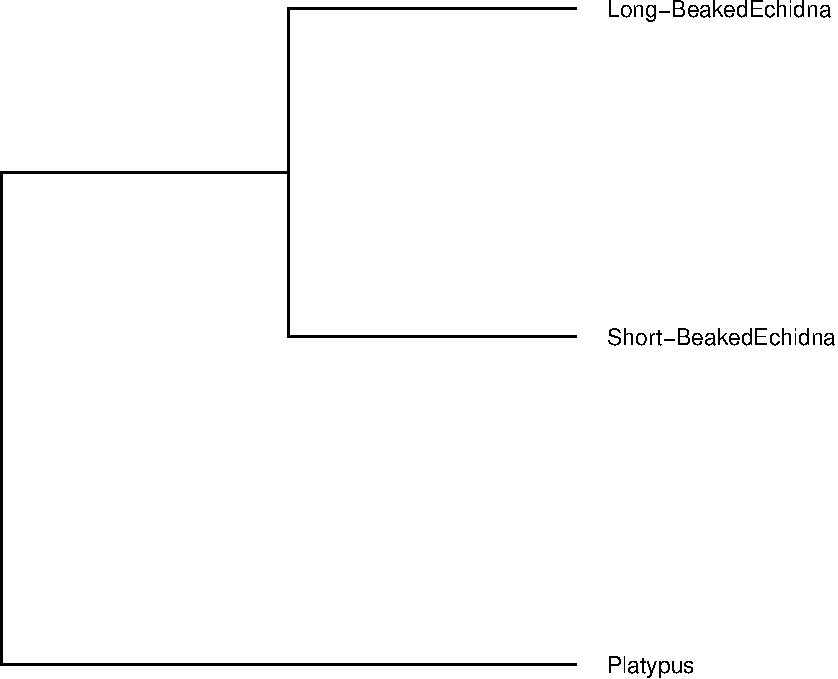
\includegraphics{bookdown-demo_files/figure-latex/unnamed-chunk-27-1} \end{center}

In reality, we know what the branch lengths should be so we can edit the \textbf{monotremes} object to include appropriate \textbf{edge.length} values.

\begin{Shaded}
\begin{Highlighting}[]
\NormalTok{monotremes}\OperatorTok{$}\NormalTok{edge.length\textless{}{-}}\KeywordTok{c}\NormalTok{(}\FloatTok{53.0}\NormalTok{,}\FloatTok{10.6}\NormalTok{,}\FloatTok{10.6}\NormalTok{,}\FloatTok{63.6}\NormalTok{)}
\KeywordTok{ggtree}\NormalTok{(monotremes) }\OperatorTok{+}
\StringTok{  }\KeywordTok{geom\_tiplab}\NormalTok{(}\DataTypeTok{offset =} \FloatTok{.1}\NormalTok{) }\OperatorTok{+}
\StringTok{  }\KeywordTok{xlim}\NormalTok{(}\DecValTok{0}\NormalTok{,}\DecValTok{80}\NormalTok{)}
\end{Highlighting}
\end{Shaded}

\begin{center}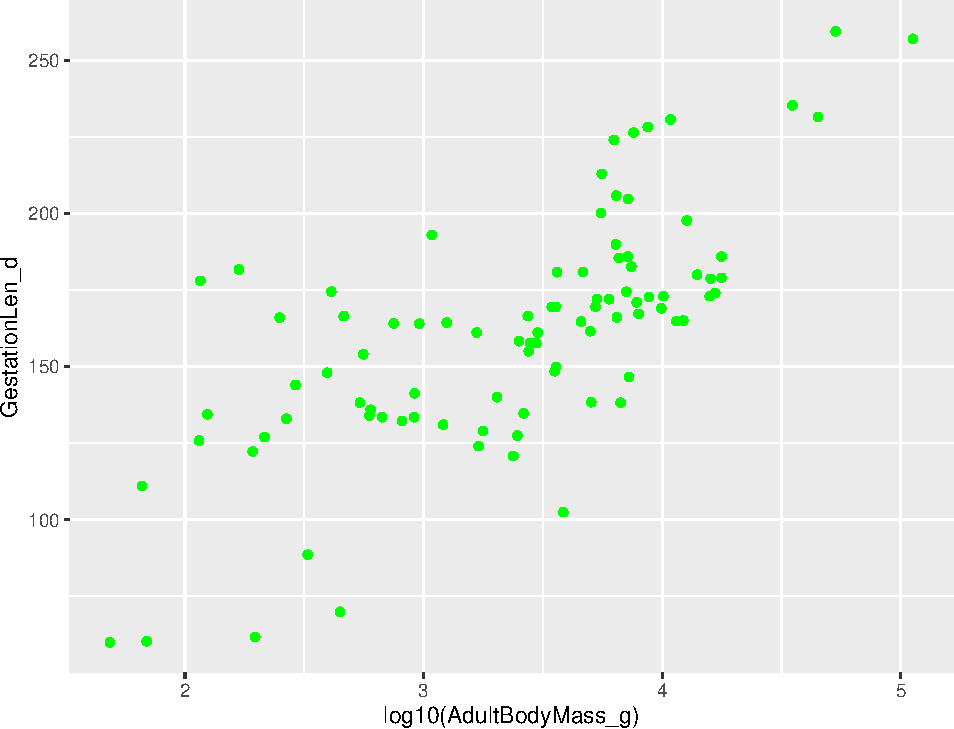
\includegraphics{bookdown-demo_files/figure-latex/unnamed-chunk-28-1} \end{center}

In Newick format, these branch lengths would be represented with a colon and the length of the branch as follows.

\[ ((\text{Short-beaked echidna: 10.6 , Long-beaked echidna: 10.6})\text{: 53.0, Platypus: 63.6}); \]

Of course, trees with more species will be much more complex but they will follow this basic format.

R stores phylogenies as objects of class \textbf{Phylo}. In the simplest case, this class of object is a list of four elements. \textbf{edge} refers to the branches. \textbf{Nnode} is the number of internal nodes. \textbf{tip.label} is a list of the tip labels (usually species names). \textbf{edge.length} is the list of branch lengths.

\begin{Shaded}
\begin{Highlighting}[]
\KeywordTok{str}\NormalTok{(monotremes)}
\end{Highlighting}
\end{Shaded}

\begin{verbatim}
List of 4
 $ edge       : int [1:4, 1:2] 4 5 5 4 5 1 2 3
 $ Nnode      : int 2
 $ tip.label  : chr [1:3] "Short-BeakedEchidna" "Long-BeakedEchidna" "Platypus"
 $ edge.length: num [1:4] 53 10.6 10.6 63.6
 - attr(*, "class")= chr "phylo"
 - attr(*, "order")= chr "cladewise"
\end{verbatim}

There is another common way phylogenies are stored within R. This is an object of class \textbf{MultiPhylo}. This class of object is essentially a list of objects of class Phylo. This is a common way of storing the results of phylogenetic inferences with some uncertainty. Modern phylogentic methods often produce thousands of trees which all differ very slightly, thus preserving appropriate uncertainty in things like branch lengths and topology.

\hypertarget{finding-trees}{%
\section{Finding trees}\label{finding-trees}}

There are many places to access publically available phylogenetic trees. This is a non-exhaustive summary of some of the more familiar ones.

\hypertarget{vertlife}{%
\subsection{Vertlife}\label{vertlife}}

\href{https://vertlife.org/}{Vertlife} is a website funded by the National Science Foundation which provides species-level phylogenies for terrestrial vertebrates. The website is the product of a great deal of work from multiple projects at multiple institutes. What they have created is one of the best resources anywhere for a comparative biologist!

If you navigate to the \href{https://vertlife.org/phylosubsets/}{phylogeny subsets} section of the website, you will see that you can get trees covering \textbf{amphibians}, \textbf{birds}, \textbf{mammals}, \textbf{sharks} and \textbf{squamates} simply by pasting the list of species you want into the window. The trees will be emailed you as soon as they are ready.

This website contains probably the most complete coverage I am aware of for some lineages. Particularly for mammals and birds (two commonly used study groups), the taxonomic coverage is excellent.

\hypertarget{ktrees}{%
\subsection{10ktrees}\label{ktrees}}

The \href{https://10ktrees.nunn-lab.org/}{10ktrees} project is similar to Vertlife but restricted to a few lineages of mammal. Namely, this website deals with primates, perissodactyls (odd-toed ungulates), cetartiodactyls (even-toed ungulated and cetaceans) and carnivorans.

These trees are built in a similar methodology to Vertlife (which is more up to date) so you may be better off going to Vertlife for these species. It may be interesting however if you would like to compare the differences between the 10ktrees phylogeny and the Vertlife phylogeny.

\hypertarget{treebase}{%
\subsection{TreeBASE}\label{treebase}}

\href{https://www.treebase.org/treebase-web/home.html}{TreeBASE} is a searchable database of papers that have built phylogenetic trees. The search engine built into the site allows you to search by author, title, DOI, abstract and study ID (if you know it). You can also search by the entire citation if you aren't sure which study you are looking for. There are also options to search by tree ID and taxa if you know what you are looking for!

\hypertarget{primary-literature}{%
\subsection{Primary literature}\label{primary-literature}}

There are many studies that have sought to build phylogenetic trees for a given lineage. Many of these papers provide the trees for use in the \textbf{supplementary information} section of the online publication.

As an example, Figueroa \emph{et al}. \citeyearpar{Figueroa16} constructed a species-level phylogeny of snakes, covering 1745 species. The tree is provided in Newick format \href{https://doi.org/10.1371/journal.pone.0161070.s003}{here}. In this case, the Newick text is provided as a Microsoft Word document. To make this readable by R, we can simply copy and paste the Newick text into a .txt file and read it in using \textbf{read.newick} from the \textbf{phytools} package \citep{phytools}.

\begin{Shaded}
\begin{Highlighting}[]
\KeywordTok{library}\NormalTok{(phytools)}
\NormalTok{snakes \textless{}{-}}\StringTok{ }\KeywordTok{read.newick}\NormalTok{(}\StringTok{"snakes.txt"}\NormalTok{)}
\KeywordTok{ggtree}\NormalTok{(snakes)}
\end{Highlighting}
\end{Shaded}

\begin{center}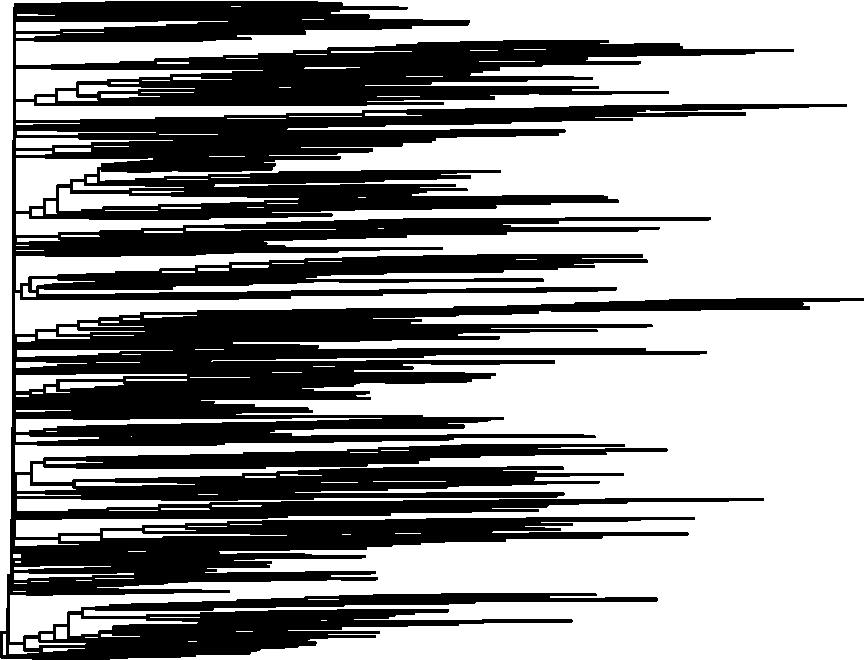
\includegraphics{bookdown-demo_files/figure-latex/unnamed-chunk-31-1} \end{center}

When taking trees from the literature like this, always cite the source of the tree and make sure you are aware of how and why the tree was built. If the tree has been surpassed by subsequent publications or is the subject of ongoing debate in the literature, this is important to be aware of when interpreting results arrived at using the tree.

\hypertarget{tree.drawer}{%
\subsection{tree.drawer}\label{tree.drawer}}

Sometimes, a tree used in a study will not be provided in an easily usable format. In some cases, it may only be provided as a figure in a paper.

When this happens, all is not lost! Liam Revell has developed a function called \textbf{tree.drawer} within phytools which allows us to trace over a tree \citep{phytools}. Simply load the image into R using the \textbf{jpeg} package \citep{jpeg} and trace the tree by pointing and clicking on the graphics window. A full tutorial with examples is available \href{http://blog.phytools.org/2017/01/second-video-demo-of-treedrawer-in.html}{here}.

\hypertarget{further-info}{%
\section{Further info}\label{further-info}}

For more information about phylogenetics in general, the main text (and a very readble source) is \emph{Tree Thinking: An introduction to phylogenetic biology} \citep{baum12}.

\hypertarget{w1plotting}{%
\chapter{Plotting trees in R}\label{w1plotting}}

\hypertarget{phylogenies-in-r}{%
\section{Phylogenies in R}\label{phylogenies-in-r}}

From LIFE223, you know R as a powerful statistical tool. You will also be aware that it is an incredibly flexible tool for plotting data. In this workshop, we will be working with phylogenies in R and manipulating them to produce informative plots.

\hypertarget{packages-used}{%
\subsection{Packages used}\label{packages-used}}

In this section we'll mostly be using a package called ggtree \citep{Yu17, Yu18}. To install it, we need another package called \textbf{BiocManager} \citep{Morgan19}.

\begin{Shaded}
\begin{Highlighting}[]
\KeywordTok{install.packages}\NormalTok{(}\StringTok{"BiocManager"}\NormalTok{)}
\NormalTok{BiocManager}\OperatorTok{::}\KeywordTok{install}\NormalTok{(}\StringTok{"ggtree"}\NormalTok{)}
\KeywordTok{library}\NormalTok{(ggtree)}
\end{Highlighting}
\end{Shaded}

We will also need to use phylobase \citep{phylobase}, ggimage \citep{Yu19} and it would help to have the tidyverse packages loaded \citep{Wickham17} since we'll be using the syntax of ggplot2. If you get an error message, make sure the packages are installed first.

\begin{Shaded}
\begin{Highlighting}[]
\KeywordTok{library}\NormalTok{(tidyverse)}
\KeywordTok{library}\NormalTok{(phylobase)}
\KeywordTok{library}\NormalTok{(ggimage)}
\end{Highlighting}
\end{Shaded}

\hypertarget{importing-your-tree}{%
\section{Importing your tree}\label{importing-your-tree}}

Let's start by importing a tree. Make sure your working directory is set to wherever you have saved the tree\_newick file. If you run this line, you should see an object called ``tree'' appear in your global environment.

\begin{Shaded}
\begin{Highlighting}[]
\NormalTok{tree \textless{}{-}}\StringTok{ }\KeywordTok{read.tree}\NormalTok{(}\StringTok{"tree\_newick.nwk"}\NormalTok{)}
\end{Highlighting}
\end{Shaded}

If we take a look at the structure of our tree object using the \textbf{str} function we can see that the tree is stored as an object of class \textbf{Phylo}. If you are using a block of trees (more on this subsequent chapters) it will be an object of class \textbf{Multiphylo}.

\begin{Shaded}
\begin{Highlighting}[]
\KeywordTok{str}\NormalTok{(tree)}
\end{Highlighting}
\end{Shaded}

\begin{verbatim}
List of 4
 $ edge       : int [1:24, 1:2] 14 15 16 17 18 19 20 20 19 18 ...
 $ edge.length: num [1:24] 4 13 10 3 8 6 4 4 5 6 ...
 $ Nnode      : int 12
 $ tip.label  : chr [1:13] "A" "B" "C" "D" ...
 - attr(*, "class")= chr "phylo"
 - attr(*, "order")= chr "cladewise"
\end{verbatim}

We can see a list of 4 elements of the tree object. The first (\textbf{edge}) contains the edges (also known as branches) of the phylogeny and their labels. The next is \textbf{edge.length} which contains the lengths of the branches if present (see \textbf{chapter 3} for more details). \textbf{Nnode} specifies the number of nodes and finally \textbf{tip.label} contains the labels of the tips. In this case, we just have letters for tip labels.

Things are often clearer when we plot them. We can do this for trees with the \textbf{plot} function in base R. This function is incredibly versatile and you should recognise it from LIFE223. Here we are using very different arguments.

\begin{Shaded}
\begin{Highlighting}[]
\KeywordTok{plot}\NormalTok{(tree)}
\end{Highlighting}
\end{Shaded}

\begin{center}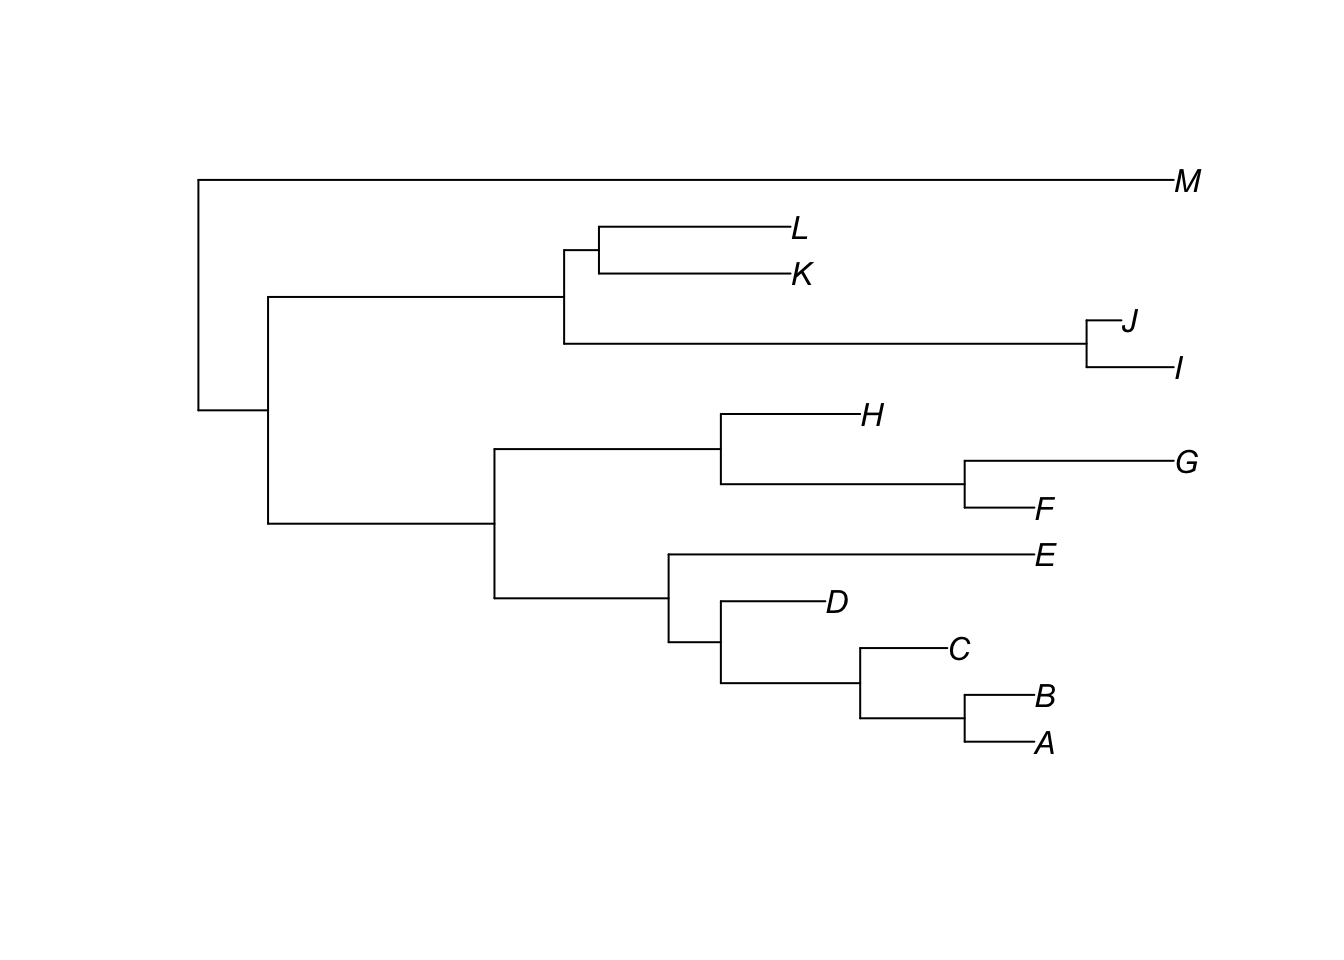
\includegraphics{bookdown-demo_files/figure-latex/unnamed-chunk-39-1} \end{center}

This plot is fine for a quick check to make sure the tree looks as we expected it to. Let's look at making a more attractive plot with ggtree.

\hypertarget{ggtree}{%
\section{ggtree}\label{ggtree}}

The package ggtree is an extension of \textbf{ggplot2} \citep{ggplot2}, a popular plotting package from the \textbf{tidyverse} family of packages. The syntax we'll be using here is a little different that what you may be used to so don't get intimidated. \textbf{ggtree} uses the same syntax as \textbf{ggplot2}. This works by creating layers (known as \textbf{geoms}) and plotting them over each other to build up the plot.

We'll start by using ggtree to plot our tree. Below is the base layer of the plot. There are many other options we can include to customise our tree. Try some out in this R window to see how they effect your plot.

\hypertarget{geoms}{%
\subsection{Geoms}\label{geoms}}

Geoms are new layers to plot on or alongside your tree. Now let's try plotting it whilst adding new layers. These geoms can be combined as you see fit. This gives you a lot of flexibility in how you plot your trees. For example, we can add a geom to include the tip labels for our tree.

\begin{Shaded}
\begin{Highlighting}[]
\KeywordTok{ggtree}\NormalTok{(tree) }\OperatorTok{+}\StringTok{ }
\StringTok{  }\KeywordTok{geom\_tiplab}\NormalTok{()}
\end{Highlighting}
\end{Shaded}

\begin{center}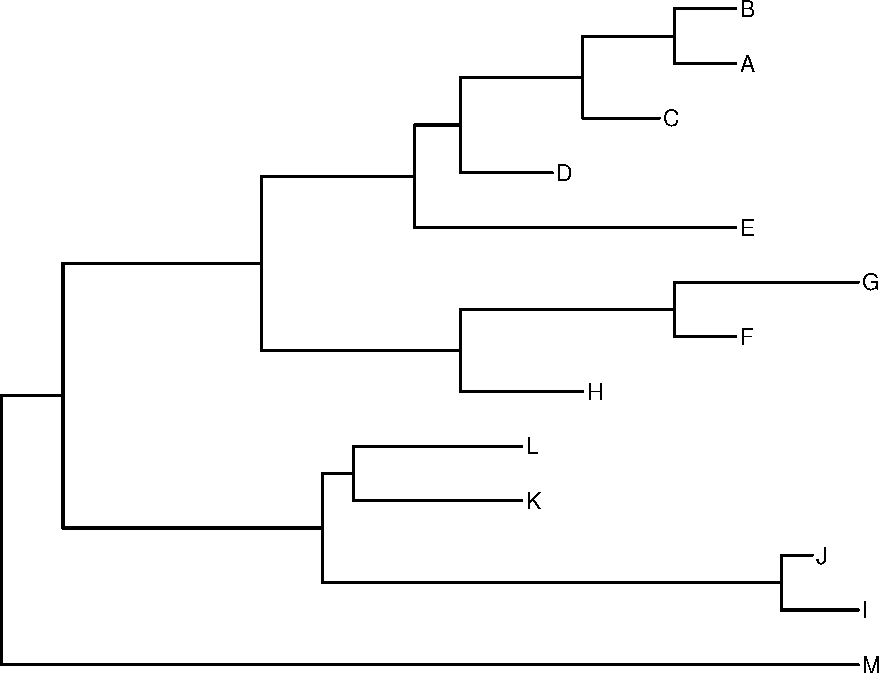
\includegraphics{bookdown-demo_files/figure-latex/unnamed-chunk-40-1} \end{center}

And we can add a title

\begin{Shaded}
\begin{Highlighting}[]
\KeywordTok{ggtree}\NormalTok{(tree) }\OperatorTok{+}\StringTok{ }
\StringTok{  }\KeywordTok{geom\_tiplab}\NormalTok{() }\OperatorTok{+}
\StringTok{  }\KeywordTok{ggtitle}\NormalTok{(}\StringTok{"A phylogeny of letters. For some reason..."}\NormalTok{)}
\end{Highlighting}
\end{Shaded}

\begin{center}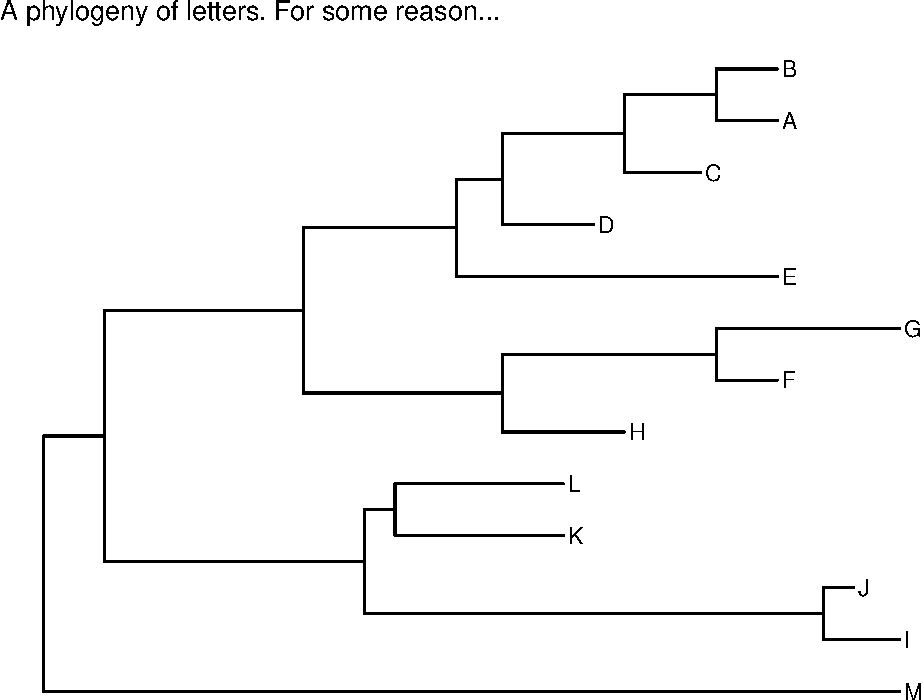
\includegraphics{bookdown-demo_files/figure-latex/unnamed-chunk-41-1} \end{center}

There are many geoms you can use to add more information to your plot. Here are just a few that you may want to investigate.

\begin{Shaded}
\begin{Highlighting}[]
\KeywordTok{geom\_tiplab}\NormalTok{() }\CommentTok{\#adds tiplabels}
\KeywordTok{geom\_tippoint}\NormalTok{() }\CommentTok{\#adds points at the tips}
\KeywordTok{geom\_nodepoint}\NormalTok{() }\CommentTok{\#adds points at the nodes}
\KeywordTok{geom\_nodelab}\NormalTok{() }\CommentTok{\#adds labels for nodes}
\KeywordTok{geom\_cladelabel}\NormalTok{() }\CommentTok{\#adds labels for clades}
\end{Highlighting}
\end{Shaded}

\hypertarget{labelling-clades}{%
\subsection{Labelling clades}\label{labelling-clades}}

As an example of what you might like to do with ggtree, let's have a look at adding some labels to identify some clades on our tree. To label clades, we need to be able to identify the node of the most recent common ancestor. The function \textbf{MRCA} in the package \textbf{phylobase} \citep{phylobase} tells us that the common ancestor of C and E is node 17.

\begin{Shaded}
\begin{Highlighting}[]
\NormalTok{phylobase}\OperatorTok{::}\KeywordTok{MRCA}\NormalTok{(tree, }\DataTypeTok{tip =} \KeywordTok{c}\NormalTok{(}\StringTok{"C"}\NormalTok{, }\StringTok{"E"}\NormalTok{))}
\end{Highlighting}
\end{Shaded}

\begin{verbatim}
[1] 17
\end{verbatim}

We can now use the \textbf{geom\_cladelabel} geom to add a simple label for the clade descended from the appropriate node. Take note of the arguments I've added to customise the geom. You may want to play around with these options yourself to see how they work.

\begin{Shaded}
\begin{Highlighting}[]
\KeywordTok{ggtree}\NormalTok{(tree) }\OperatorTok{+}\StringTok{ }
\StringTok{  }\KeywordTok{geom\_tiplab}\NormalTok{() }\OperatorTok{+}\StringTok{ }
\StringTok{  }\KeywordTok{geom\_cladelabel}\NormalTok{(}\DataTypeTok{node=}\DecValTok{17}\NormalTok{, }\DataTypeTok{label=}\StringTok{"A clade"}\NormalTok{, }
                  \DataTypeTok{color=}\StringTok{"red2"}\NormalTok{, }\DataTypeTok{offset=}\DecValTok{1}\NormalTok{)}
\end{Highlighting}
\end{Shaded}

\begin{center}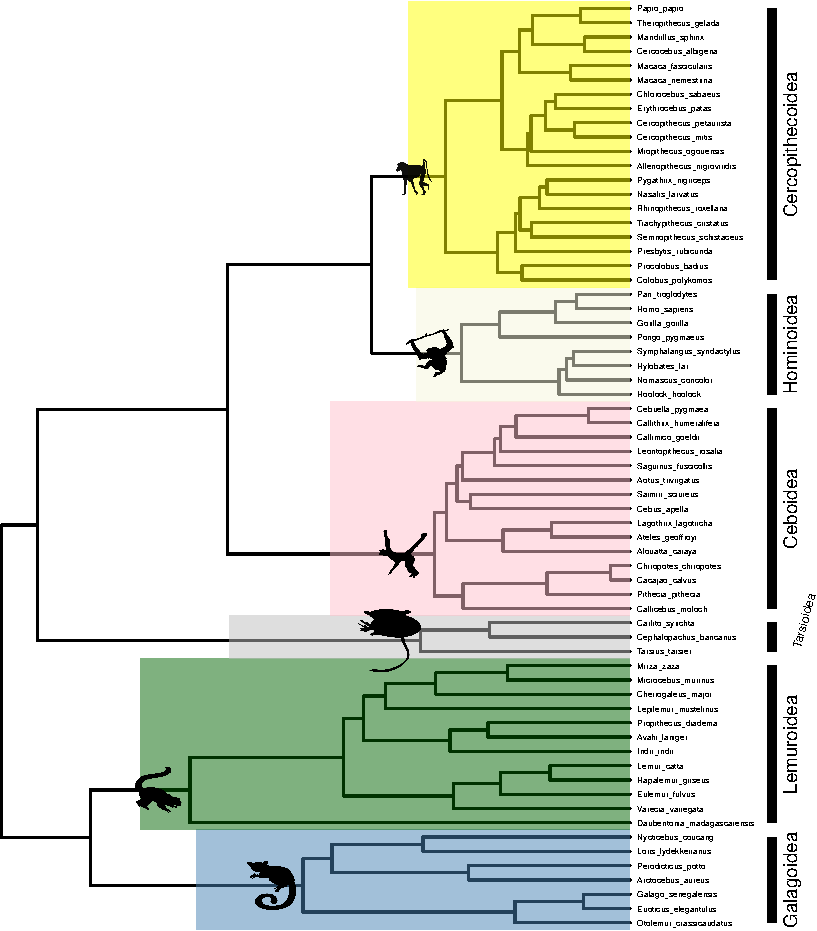
\includegraphics{bookdown-demo_files/figure-latex/unnamed-chunk-44-1} \end{center}

Pretty good but there are other options. This is a matter of personal preference. You may prefer to overlay a translucent rectangle over your clade of interest.

\begin{Shaded}
\begin{Highlighting}[]
\KeywordTok{ggtree}\NormalTok{(tree) }\OperatorTok{+}\StringTok{ }
\StringTok{  }\KeywordTok{geom\_tiplab}\NormalTok{() }\OperatorTok{+}\StringTok{ }
\StringTok{  }\KeywordTok{geom\_hilight}\NormalTok{(}\DataTypeTok{node=}\DecValTok{17}\NormalTok{, }\DataTypeTok{fill=}\StringTok{"gold"}\NormalTok{)}
\end{Highlighting}
\end{Shaded}

\begin{center}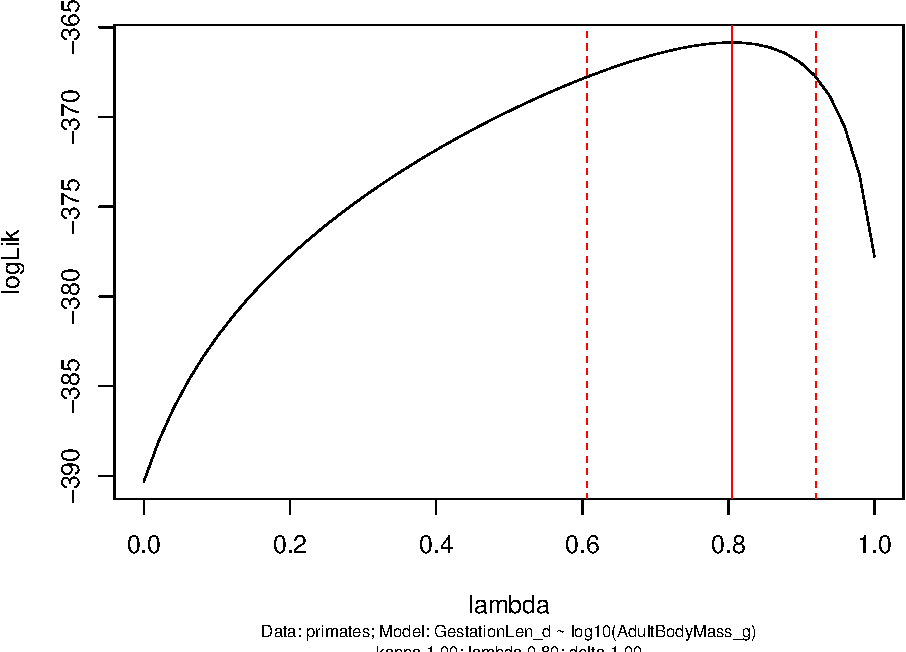
\includegraphics{bookdown-demo_files/figure-latex/unnamed-chunk-45-1} \end{center}

Use the R window below to experiment with the available geoms in ggtree. Find a combination that suits you and your tree.

\hypertarget{adding-images-to-trees}{%
\section{Adding images to trees}\label{adding-images-to-trees}}

As you probably noted in chapter 3, adding images to a plot is an excellent way to annotate your tree. The ggtree package can do this as you can see here.

\begin{figure}[H]

{\centering 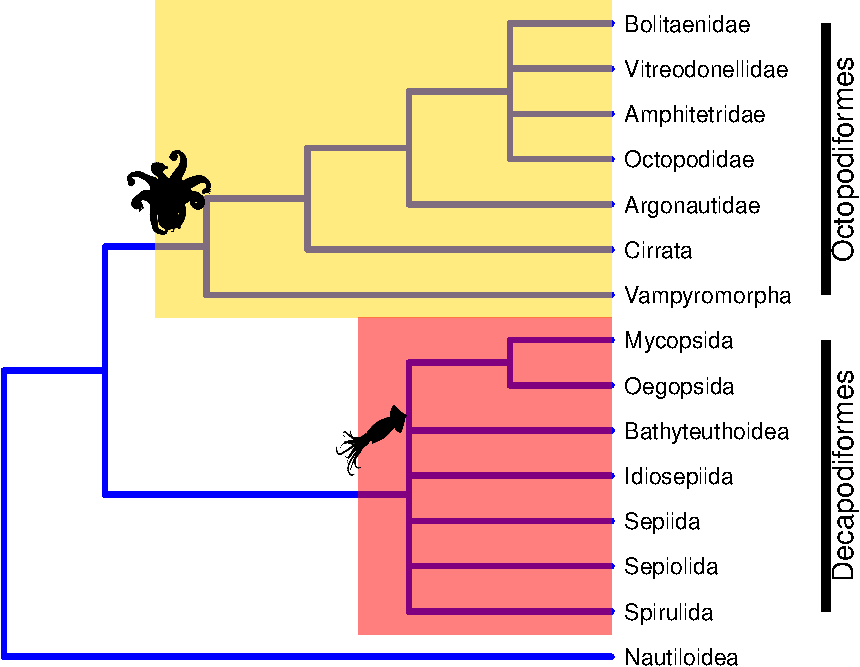
\includegraphics{bookdown-demo_files/figure-latex/unnamed-chunk-46-1} 

}

\caption{Plot of cephalopod families annotated using ggtree and Phylopic.}\label{fig:unnamed-chunk-46}
\end{figure}

This phylogeny is annotated in a number of useful ways. The tip labels describe cephalopod families. The superorders (octopodiformes and decapodiformes) are highlighted by gold and red rectangles as well as a bar across the tips. this demonstrates how multiple geoms can combine to make a plot easy to interpret.

The most interesting thing for our purposes are the silhouettes at the root of each superorder. The octopodiformes have an octopus and the decapodiformes have a squid as example taxa from within the superorder.

\hypertarget{phylopic}{%
\subsection{Phylopic}\label{phylopic}}

The silhouettes used for that plot are from a website called \href{http://phylopic.org/}{Phylopic}. Phylopic provides open source biological silhouettes that are free to use. We're now going to look at how to get these silhouettes and use them to annotate our trees.

Let's start with loading an example tree. This one is a primate tree courtesy of \href{https://www.randigriffin.com/}{Randi Griffin}. You'll notice that I'm loading this tree using a url. This is because I'm loading a file directly from GitHub, a repository for all sorts of code and the host of this site! Randi (and many other coders) make some of the things they produce freely available through GitHub. This can be data, files or code.

\begin{Shaded}
\begin{Highlighting}[]
\NormalTok{primates \textless{}{-}}\StringTok{ }\KeywordTok{read.nexus}\NormalTok{(}\StringTok{"https://raw.githubusercontent.com/rgriff23/Dissertation/master/Chapter\_2/data/tree.nex"}\NormalTok{)}
\end{Highlighting}
\end{Shaded}

Let's plot the new tree first. Here I'm assigning the plot to a named object (\textbf{p1}) in R. This means that instead of immediately printing out the plot, R stores it in the working directory. The reason for doing this will become clear as we go on. It saves us typing out every line of code each time we want to add a new geom!

\begin{Shaded}
\begin{Highlighting}[]
\NormalTok{p1 \textless{}{-}}\StringTok{ }\KeywordTok{ggtree}\NormalTok{(primates)}
\NormalTok{p1}
\end{Highlighting}
\end{Shaded}

\begin{center}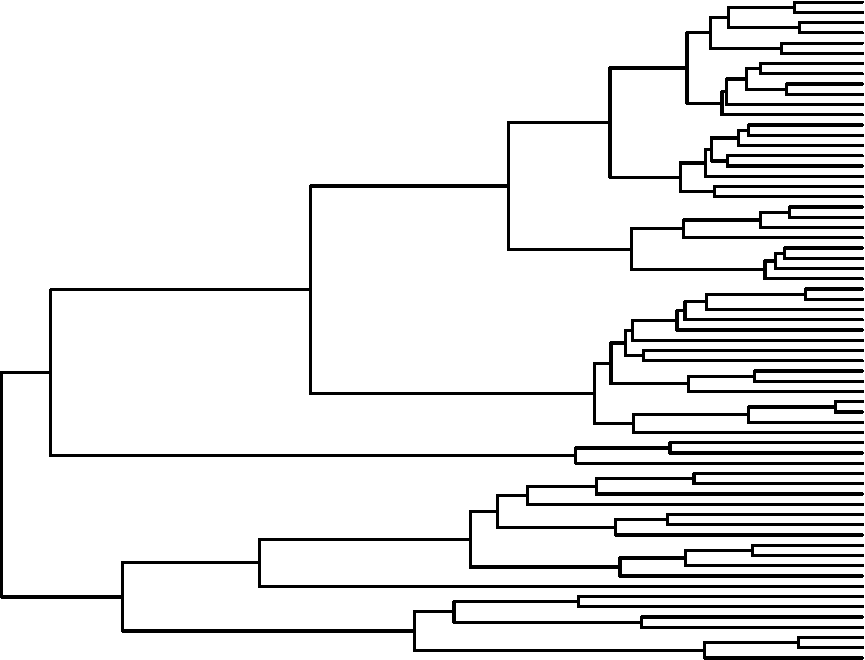
\includegraphics{bookdown-demo_files/figure-latex/unnamed-chunk-49-1} \end{center}

Let's use what we already know about ggtree to customise this plot into something more useful. In particular, this plot is quite useful because it tells us the numbers of each node and we will need that later on.

\begin{Shaded}
\begin{Highlighting}[]
\KeywordTok{ggtree}\NormalTok{(primates) }\OperatorTok{+}
\StringTok{   }\KeywordTok{xlim}\NormalTok{(}\DecValTok{0}\NormalTok{,}\DecValTok{90}\NormalTok{) }\OperatorTok{+}\StringTok{ }
\StringTok{   }\KeywordTok{geom\_tiplab}\NormalTok{(}\DataTypeTok{size=}\FloatTok{1.5}\NormalTok{) }\OperatorTok{+}
\StringTok{   }\KeywordTok{geom\_label2}\NormalTok{(}\KeywordTok{aes}\NormalTok{(}\DataTypeTok{subset=}\OperatorTok{!}\NormalTok{isTip, }\DataTypeTok{label=}\NormalTok{node), }\DataTypeTok{size=}\DecValTok{2}\NormalTok{, }\DataTypeTok{color=}\StringTok{"darkred"}\NormalTok{, }\DataTypeTok{alpha=}\FloatTok{0.5}\NormalTok{)}
\end{Highlighting}
\end{Shaded}

\begin{center}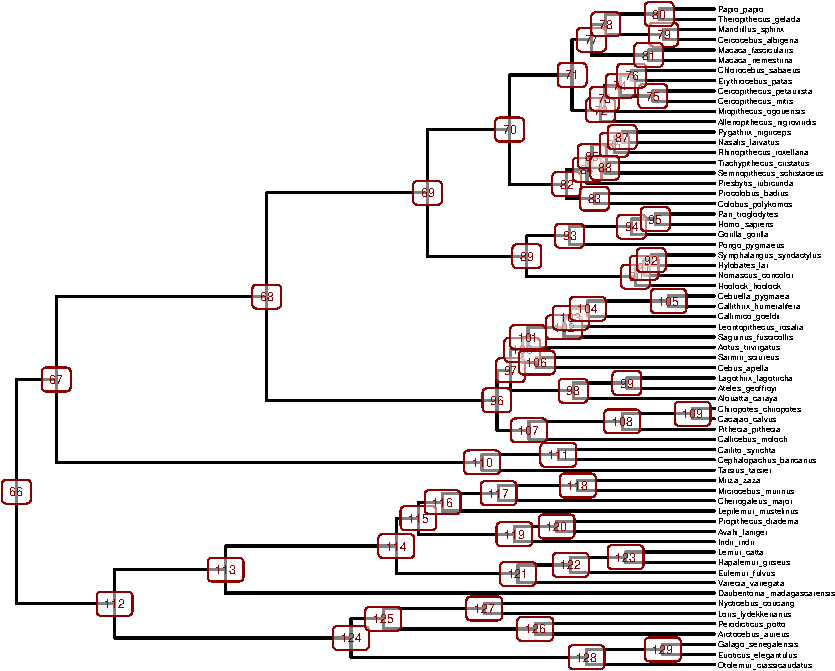
\includegraphics{bookdown-demo_files/figure-latex/unnamed-chunk-50-1} \end{center}

Let's label the 6 primate superfamilies using the node numbers I have extracted from the previous plot. You can choose whatever colours you prefer here. I've also added some useful features to this code. the use of \textbf{xlim()} can be very useful when plotting a tree with some extra space for more details. Here I've set the limits of the x dimension (the horizontal) to be between 0 and 100. This gives me space for later annotations.

\begin{Shaded}
\begin{Highlighting}[]
\NormalTok{p2 \textless{}{-}}\StringTok{ }\KeywordTok{ggtree}\NormalTok{(primates) }\OperatorTok{+}
\StringTok{  }\KeywordTok{xlim}\NormalTok{(}\DecValTok{0}\NormalTok{,}\DecValTok{100}\NormalTok{) }\OperatorTok{+}
\StringTok{  }\KeywordTok{geom\_tiplab}\NormalTok{(}\DataTypeTok{size=}\FloatTok{1.5}\NormalTok{, }\DataTypeTok{offset=}\FloatTok{0.5}\NormalTok{) }\OperatorTok{+}
\StringTok{  }\KeywordTok{geom\_hilight}\NormalTok{(}\DataTypeTok{node=}\DecValTok{124}\NormalTok{, }\DataTypeTok{fill=}\StringTok{"steelblue"}\NormalTok{, }\DataTypeTok{alpha=}\FloatTok{0.5}\NormalTok{) }\OperatorTok{+}
\StringTok{  }\KeywordTok{geom\_hilight}\NormalTok{(}\DataTypeTok{node=}\DecValTok{113}\NormalTok{, }\DataTypeTok{fill=}\StringTok{"darkgreen"}\NormalTok{, }\DataTypeTok{alpha=}\FloatTok{0.5}\NormalTok{) }\OperatorTok{+}
\StringTok{  }\KeywordTok{geom\_hilight}\NormalTok{(}\DataTypeTok{node=}\DecValTok{110}\NormalTok{, }\DataTypeTok{fill=}\StringTok{"gray"}\NormalTok{, }\DataTypeTok{alpha=}\FloatTok{0.5}\NormalTok{) }\OperatorTok{+}
\StringTok{  }\KeywordTok{geom\_hilight}\NormalTok{(}\DataTypeTok{node=}\DecValTok{96}\NormalTok{, }\DataTypeTok{fill=}\StringTok{"pink"}\NormalTok{, }\DataTypeTok{alpha=}\FloatTok{0.5}\NormalTok{) }\OperatorTok{+}
\StringTok{  }\KeywordTok{geom\_hilight}\NormalTok{(}\DataTypeTok{node=}\DecValTok{89}\NormalTok{, }\DataTypeTok{fill=}\StringTok{"beige"}\NormalTok{, }\DataTypeTok{alpha=}\FloatTok{0.5}\NormalTok{) }\OperatorTok{+}
\StringTok{  }\KeywordTok{geom\_hilight}\NormalTok{(}\DataTypeTok{node=}\DecValTok{70}\NormalTok{, }\DataTypeTok{fill=}\StringTok{"yellow"}\NormalTok{, }\DataTypeTok{alpha=}\FloatTok{0.5}\NormalTok{) }
\NormalTok{p2}
\end{Highlighting}
\end{Shaded}

\begin{center}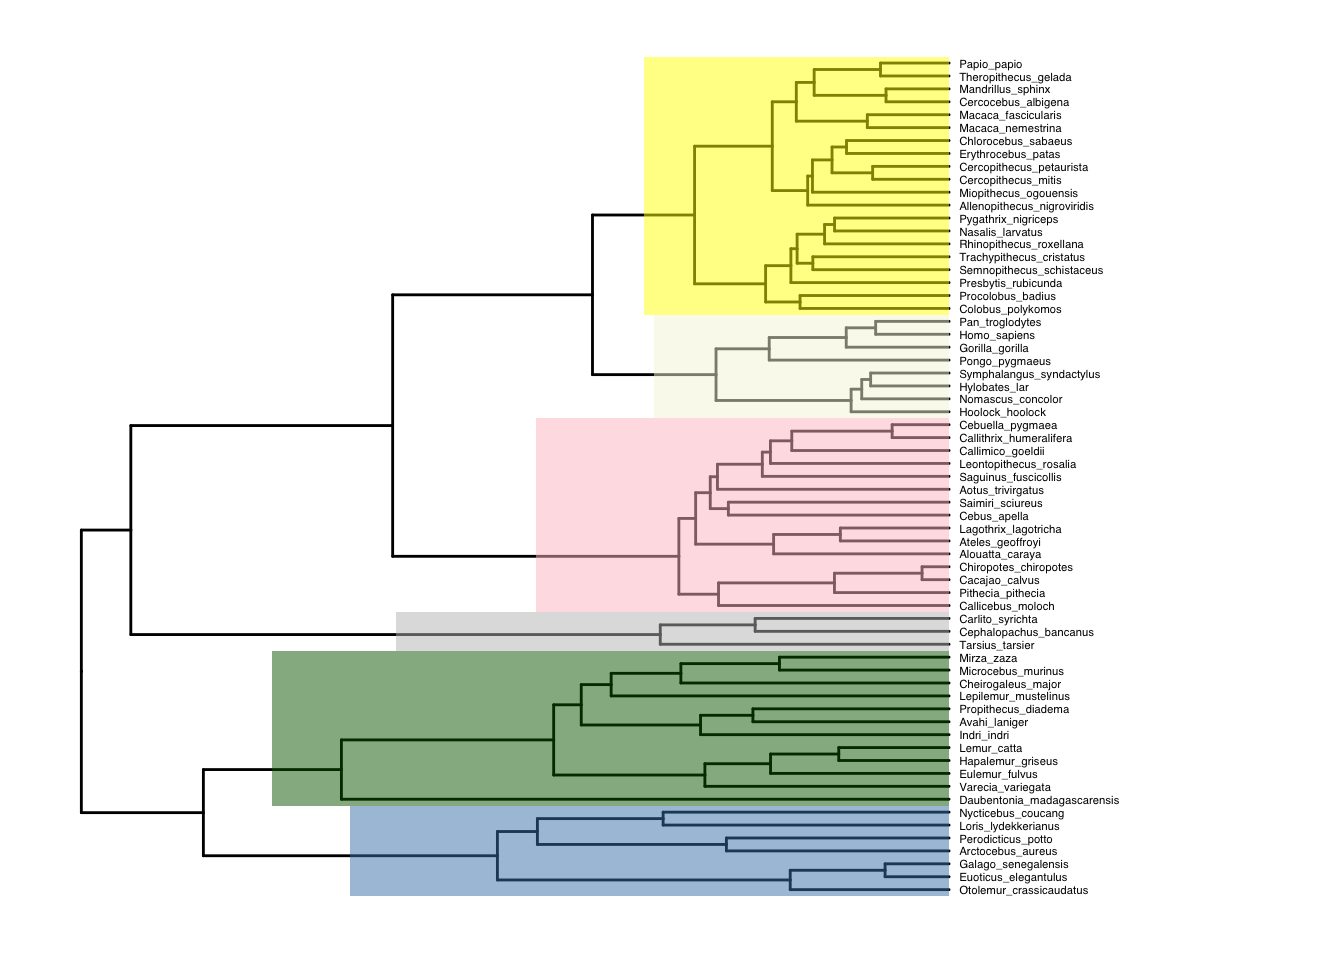
\includegraphics{bookdown-demo_files/figure-latex/unnamed-chunk-51-1} \end{center}

So far so good. Let's add on bars to label the superfamilies like I did for the cephalopod version. This time, I'll add the new details to the object p3 to save retyping. Take note of the arguments in each label. You may need to twist these with some trial-and-error to make sure they suit your plot window.

\begin{Shaded}
\begin{Highlighting}[]
\NormalTok{p3 \textless{}{-}}\StringTok{ }\NormalTok{p2 }\OperatorTok{+}
\StringTok{  }\KeywordTok{geom\_cladelabel}\NormalTok{(}\DecValTok{124}\NormalTok{, }\StringTok{"Galagoidea"}\NormalTok{, }\DataTypeTok{offset=}\DecValTok{15}\NormalTok{, }\DataTypeTok{barsize=}\DecValTok{2}\NormalTok{, }\DataTypeTok{angle=}\DecValTok{90}\NormalTok{,}
                  \DataTypeTok{offset.text=}\FloatTok{1.5}\NormalTok{, }\DataTypeTok{hjust=}\FloatTok{0.5}\NormalTok{, }\DataTypeTok{fontsize=}\DecValTok{3}\NormalTok{) }\OperatorTok{+}\StringTok{ }
\StringTok{  }\KeywordTok{geom\_cladelabel}\NormalTok{(}\DecValTok{113}\NormalTok{, }\StringTok{"Lemuroidea"}\NormalTok{, }\DataTypeTok{offset=}\DecValTok{15}\NormalTok{, }\DataTypeTok{barsize=}\DecValTok{2}\NormalTok{, }\DataTypeTok{angle=}\DecValTok{90}\NormalTok{,}
                  \DataTypeTok{offset.text=}\FloatTok{1.5}\NormalTok{, }\DataTypeTok{hjust=}\FloatTok{0.5}\NormalTok{, }\DataTypeTok{fontsize=}\DecValTok{3}\NormalTok{) }\OperatorTok{+}
\StringTok{  }\KeywordTok{geom\_cladelabel}\NormalTok{(}\DecValTok{110}\NormalTok{, }\StringTok{"Tarsioidea"}\NormalTok{, }\DataTypeTok{offset=}\DecValTok{15}\NormalTok{, }\DataTypeTok{barsize=}\DecValTok{2}\NormalTok{, }\DataTypeTok{angle=}\DecValTok{75}\NormalTok{,}
                  \DataTypeTok{offset.text=}\FloatTok{2.5}\NormalTok{, }\DataTypeTok{hjust=}\FloatTok{0.2}\NormalTok{, }\DataTypeTok{fontsize=}\DecValTok{2}\NormalTok{) }\OperatorTok{+}
\StringTok{  }\KeywordTok{geom\_cladelabel}\NormalTok{(}\DecValTok{96}\NormalTok{, }\StringTok{"Ceboidea"}\NormalTok{, }\DataTypeTok{offset=}\DecValTok{15}\NormalTok{, }\DataTypeTok{barsize=}\DecValTok{2}\NormalTok{, }\DataTypeTok{angle=}\DecValTok{90}\NormalTok{,}
                  \DataTypeTok{offset.text=}\FloatTok{1.5}\NormalTok{, }\DataTypeTok{hjust=}\FloatTok{0.5}\NormalTok{, }\DataTypeTok{fontsize=}\DecValTok{3}\NormalTok{) }\OperatorTok{+}
\StringTok{  }\KeywordTok{geom\_cladelabel}\NormalTok{(}\DecValTok{89}\NormalTok{, }\StringTok{"Hominoidea"}\NormalTok{, }\DataTypeTok{offset=}\DecValTok{15}\NormalTok{, }\DataTypeTok{barsize=}\DecValTok{2}\NormalTok{, }\DataTypeTok{angle=}\DecValTok{90}\NormalTok{,}
                  \DataTypeTok{offset.text=}\FloatTok{1.5}\NormalTok{, }\DataTypeTok{hjust=}\FloatTok{0.5}\NormalTok{, }\DataTypeTok{fontsize=}\DecValTok{3}\NormalTok{) }\OperatorTok{+}
\StringTok{  }\KeywordTok{geom\_cladelabel}\NormalTok{(}\DecValTok{70}\NormalTok{, }\StringTok{"Cercopithecoidea"}\NormalTok{, }\DataTypeTok{offset=}\DecValTok{15}\NormalTok{, }\DataTypeTok{barsize=}\DecValTok{2}\NormalTok{, }\DataTypeTok{angle=}\DecValTok{90}\NormalTok{,}
                  \DataTypeTok{offset.text=}\FloatTok{1.5}\NormalTok{, }\DataTypeTok{hjust=}\FloatTok{0.5}\NormalTok{, }\DataTypeTok{fontsize=}\DecValTok{3}\NormalTok{)}
\NormalTok{p3}
\end{Highlighting}
\end{Shaded}

\begin{center}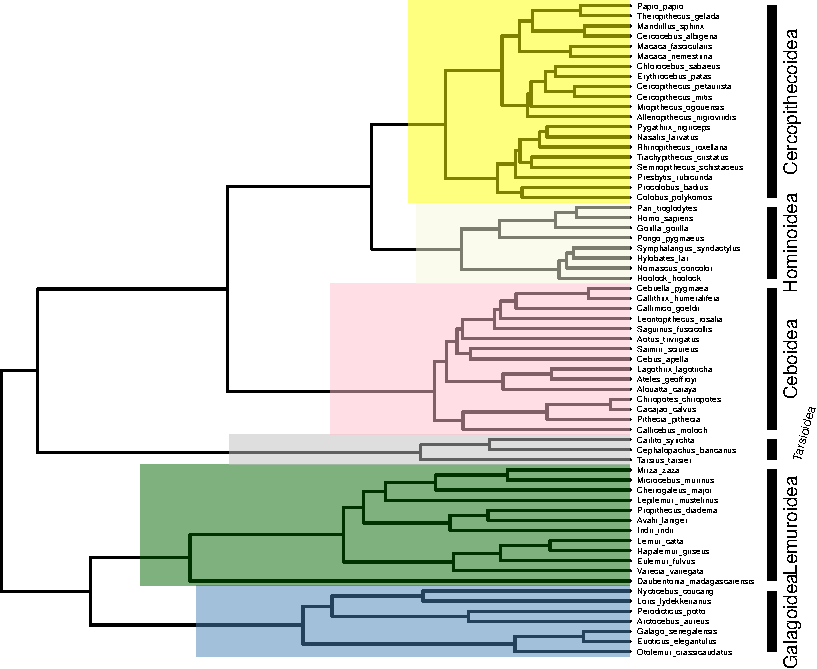
\includegraphics{bookdown-demo_files/figure-latex/unnamed-chunk-52-1} \end{center}

There are some helpful details here, such as the fact that the label for Tarsioidea is off at an angle to avoid overlapping with other labels (\textbf{angle = 75}). The extra arguments in these options demonstrate how much control you can exercise over each geom.

Now let's get to adding images. The way to do this is a little awkward but I think it's worth the hassle. The first thing we have to do is gather the links for each image we want to use. I've chosen to do this by building a small data frame containing the urls to the images on phylopic, the names of the super families I want to label and the nodes I want to plot the images on.

\begin{Shaded}
\begin{Highlighting}[]
\NormalTok{images \textless{}{-}}\StringTok{ }\KeywordTok{data.frame}\NormalTok{(}\DataTypeTok{node =} \KeywordTok{c}\NormalTok{(}\DecValTok{124}\NormalTok{,}\DecValTok{113}\NormalTok{,}\DecValTok{110}\NormalTok{,}\DecValTok{96}\NormalTok{,}\DecValTok{89}\NormalTok{,}\DecValTok{70}\NormalTok{),}
\DataTypeTok{phylopic =} \KeywordTok{c}\NormalTok{(}\StringTok{"http://phylopic.org/assets/images/submissions/}
\StringTok{7fb9bea8{-}e758{-}4986{-}afb2{-}95a2c3bf983d.512.png"}\NormalTok{,}
\StringTok{"http://phylopic.org/assets/images/submissions/}
\StringTok{bac25f49{-}97a4{-}4aec{-}beb6{-}f542158ebd23.512.png"}\NormalTok{,}
\StringTok{"http://phylopic.org/assets/images/submissions/}
\StringTok{f598fb39{-}facf{-}43ea{-}a576{-}1861304b2fe4.512.png"}\NormalTok{,}
\StringTok{"http://phylopic.org/assets/images/submissions/}
\StringTok{aceb287d{-}84cf{-}46f1{-}868c{-}4797c4ac54a8.512.png"}\NormalTok{,}
\StringTok{"http://phylopic.org/assets/images/submissions/}
\StringTok{0174801d{-}15a6{-}4668{-}bfe0{-}4c421fbe51e8.512.png"}\NormalTok{,}
\StringTok{"http://phylopic.org/assets/images/submissions/}
\StringTok{72f2f854{-}f3cd{-}4666{-}887c{-}35d5c256ab0f.512.png"}\NormalTok{),}
\DataTypeTok{species =} \KeywordTok{c}\NormalTok{(}\StringTok{"Galagoidea"}\NormalTok{,}\StringTok{"Lemuroidea"}\NormalTok{,}\StringTok{"Tarsioidea"}\NormalTok{,}
\StringTok{"Ceboidea"}\NormalTok{,}\StringTok{"Hominoidea"}\NormalTok{,}\StringTok{"Cercopithecoidea"}\NormalTok{))}
\end{Highlighting}
\end{Shaded}

Once we have the urls we need in a nice dataframe, we can pipe them into the \textbf{geom\_nodelab} geom and the end product should appear.

\begin{Shaded}
\begin{Highlighting}[]
\NormalTok{p3 }\OperatorTok{\%\textless{}+\%}\StringTok{ }\NormalTok{images }\OperatorTok{+}
\StringTok{  }\KeywordTok{geom\_nodelab}\NormalTok{(}\KeywordTok{aes}\NormalTok{(}\DataTypeTok{image =}\NormalTok{ phylopic), }\DataTypeTok{geom =} \StringTok{"image"}\NormalTok{, }\DataTypeTok{size =} \FloatTok{.04}\NormalTok{, }\DataTypeTok{nudge\_x =} \DecValTok{{-}4}\NormalTok{)}
\end{Highlighting}
\end{Shaded}

\begin{center}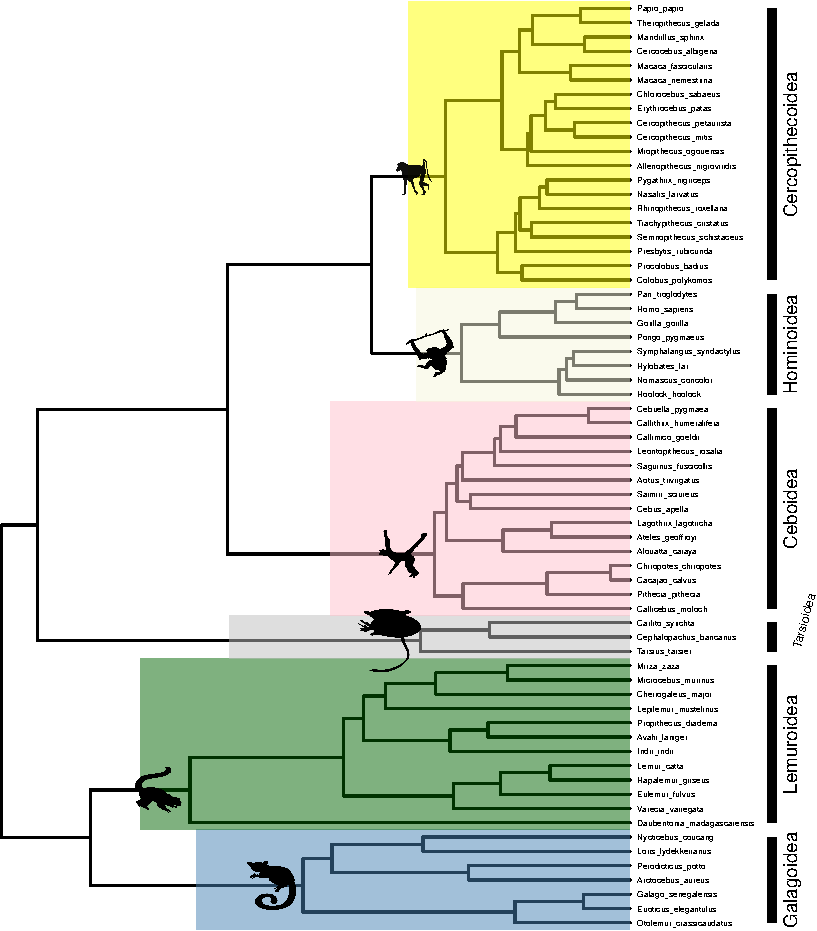
\includegraphics{bookdown-demo_files/figure-latex/unnamed-chunk-55-1} \end{center}

As you can probably tell, the images don't have to be from Phylopic. You can use any images you have the rights to in exactly the same way!

\hypertarget{further-info-1}{%
\section{Further info}\label{further-info-1}}

This chapter barely scratches the surface of what ggtree is capable of. For much more detail, have a look at Guangchuang Yu's very own Bookdown covering the topic. You can access the book by clicking \href{https://yulab-smu.github.io/treedata-book/}{here} or by running the following code in R once you have ggtree installed.

\begin{Shaded}
\begin{Highlighting}[]
\KeywordTok{vignette}\NormalTok{(}\StringTok{"ggtree"}\NormalTok{, }\DataTypeTok{package =} \StringTok{"ggtree"}\NormalTok{)}
\end{Highlighting}
\end{Shaded}

\hypertarget{anova}{%
\chapter{ANOVA}\label{anova}}

Analysis of variance (ANOVA) is something you should recognise from your quantitative skills course. This chapter will begin with a brief recap before showing you how to perform phylogenetically corrected ANOVA.

\hypertarget{analysis-of-variance}{%
\section{Analysis of variance}\label{analysis-of-variance}}

Analysis of variance asks if there are differences in the mean values between 3 or more categories. If there are only two categories (Terrestrial/Aquatic for example), then you need a t-test.

In LIFE223 you analysed the results of an experiment in which corncrake hatchlings were raised on four different supplements in addition to their normal diet.

\begin{figure}[H]

{\centering 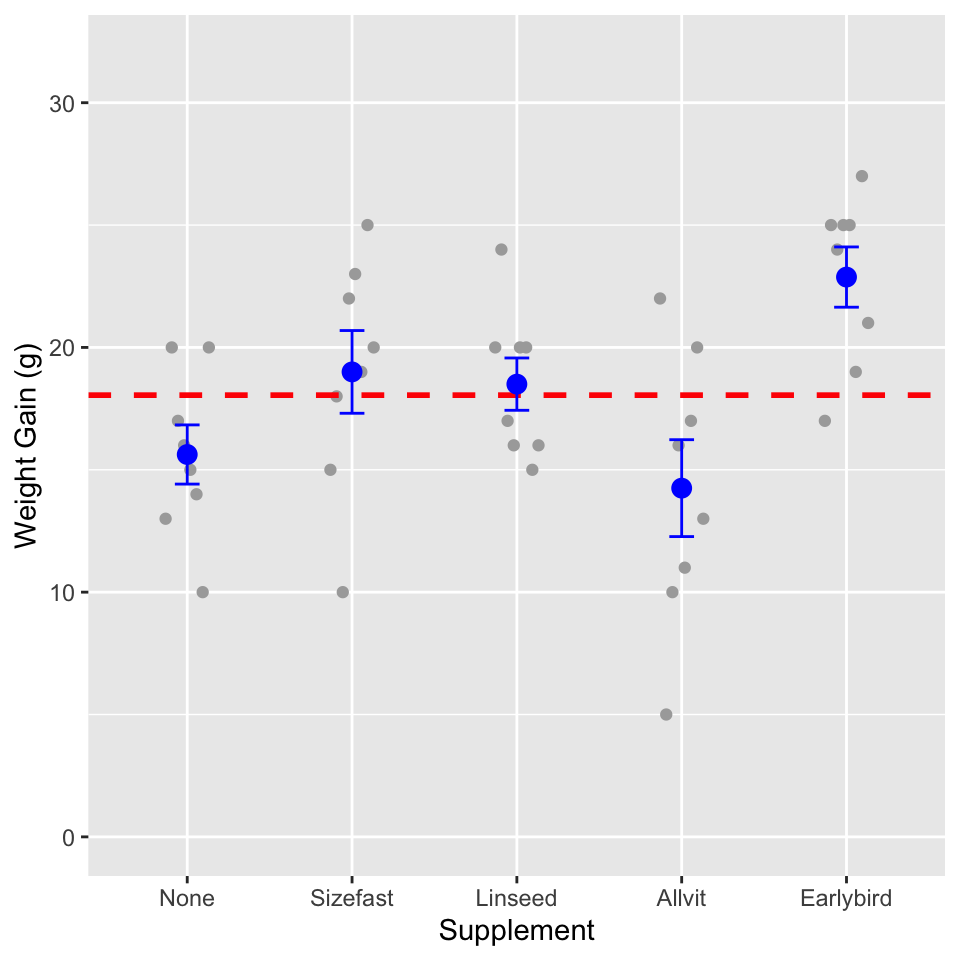
\includegraphics{bookdown-demo_files/figure-latex/unnamed-chunk-59-1} 

}

\caption{Plot of weight gain in corncrake hatchlings reared on four different nutritional supplements and a control group. The mean and standard deviation of each group is plotted in blue. The mean weight gain across the entire sample is plotted in red.}\label{fig:unnamed-chunk-59}
\end{figure}

\begin{Shaded}
\begin{Highlighting}[]
\NormalTok{corncrake.model \textless{}{-}}\StringTok{ }\KeywordTok{lm}\NormalTok{(WeightGain }\OperatorTok{\textasciitilde{}}\StringTok{ }\NormalTok{Supplement, }\DataTypeTok{data =}\NormalTok{ corncrake)}
\KeywordTok{anova}\NormalTok{(corncrake.model)}
\end{Highlighting}
\end{Shaded}

\begin{verbatim}
Analysis of Variance Table

Response: WeightGain
           Df Sum Sq Mean Sq F value   Pr(>F)   
Supplement  4 357.65  89.413  5.1281 0.002331 **
Residuals  35 610.25  17.436                    
---
Signif. codes:  0 '***' 0.001 '**' 0.01 '*' 0.05 '.' 0.1 ' ' 1
\end{verbatim}

The one-way ANOVA shows that there was a significant effect of supplement on the weight gain of the corncrake hatchlings (F = 5.1, df = 4, 35, p \textless{} 0.01). The final step is to perform our multiple comparisons test.

\begin{Shaded}
\begin{Highlighting}[]
\NormalTok{corncrake.aov \textless{}{-}}\StringTok{ }\KeywordTok{aov}\NormalTok{(corncrake.model)}
\KeywordTok{TukeyHSD}\NormalTok{(corncrake.aov, }\DataTypeTok{ordered =} \OtherTok{TRUE}\NormalTok{)}
\end{Highlighting}
\end{Shaded}

\begin{verbatim}
  Tukey multiple comparisons of means
    95% family-wise confidence level
    factor levels have been ordered

Fit: aov(formula = corncrake.model)

$Supplement
                    diff       lwr       upr     p adj
None-Allvit        1.375 -4.627565  7.377565 0.9638453
Linseed-Allvit     4.250 -1.752565 10.252565 0.2707790
Sizefast-Allvit    4.750 -1.252565 10.752565 0.1771593
Earlybird-Allvit   8.625  2.622435 14.627565 0.0018764
Linseed-None       2.875 -3.127565  8.877565 0.6459410
Sizefast-None      3.375 -2.627565  9.377565 0.4971994
Earlybird-None     7.250  1.247435 13.252565 0.0113786
Sizefast-Linseed   0.500 -5.502565  6.502565 0.9992352
Earlybird-Linseed  4.375 -1.627565 10.377565 0.2447264
Earlybird-Sizefast 3.875 -2.127565  9.877565 0.3592201
\end{verbatim}

The \textbf{TukeyHSD} functions shows us the pairwise comparisons between groups. We can see (for example) that \emph{Allvit} was not significantly different from the control (difference = 1.375g, p = 0.96) but \emph{Earlybird} was significantly better than the control group (difference = 7.25g, p = 0.01).

\hypertarget{phylogenetic-correction}{%
\section{Phylogenetic correction}\label{phylogenetic-correction}}

As you know, when trying to run a similar analysis on non-independent data (such as species) we will run into problems. Garland \emph{et al} \citeyearpar{garland93} developed a simulation based approach to solve this problem. The phylogenetic ANOVA uses computer simulations of traits evolving the phylogenetic tree. The next section contains some example data and a phylogeny to demonstrate the method.

\hypertarget{example-data-analysis}{%
\section{Example data \& analysis}\label{example-data-analysis}}

The data we're using is taken from the package \textbf{geiger} \citep{geiger} so make sure the package is installed and loaded.

\begin{Shaded}
\begin{Highlighting}[]
\KeywordTok{install.packages}\NormalTok{(}\StringTok{"geiger"}\NormalTok{)}
\KeywordTok{library}\NormalTok{(geiger)}
\end{Highlighting}
\end{Shaded}

Load the data as follows. The tree and data are stored together so we'll need to save them to separate objects called \textbf{dat} and \textbf{phy}. You probably don't \emph{need} to do this but this is more similar to what you're likely to see when using your own data.

\begin{Shaded}
\begin{Highlighting}[]
\KeywordTok{data}\NormalTok{(}\StringTok{"geospiza"}\NormalTok{)}
\NormalTok{dat \textless{}{-}}\StringTok{ }\NormalTok{geospiza}\OperatorTok{$}\NormalTok{dat}
\NormalTok{tree \textless{}{-}}\StringTok{ }\NormalTok{geospiza}\OperatorTok{$}\NormalTok{phy}
\KeywordTok{head}\NormalTok{(dat)}
\end{Highlighting}
\end{Shaded}

\begin{verbatim}
                wingL  tarsusL  culmenL    beakD   gonysW
magnirostris 4.404200 3.038950 2.724667 2.823767 2.675983
conirostris  4.349867 2.984200 2.654400 2.513800 2.360167
difficilis   4.224067 2.898917 2.277183 2.011100 1.929983
scandens     4.261222 2.929033 2.621789 2.144700 2.036944
fortis       4.244008 2.894717 2.407025 2.362658 2.221867
fuliginosa   4.132957 2.806514 2.094971 1.941157 1.845379
\end{verbatim}

\begin{figure}[H]

{\centering 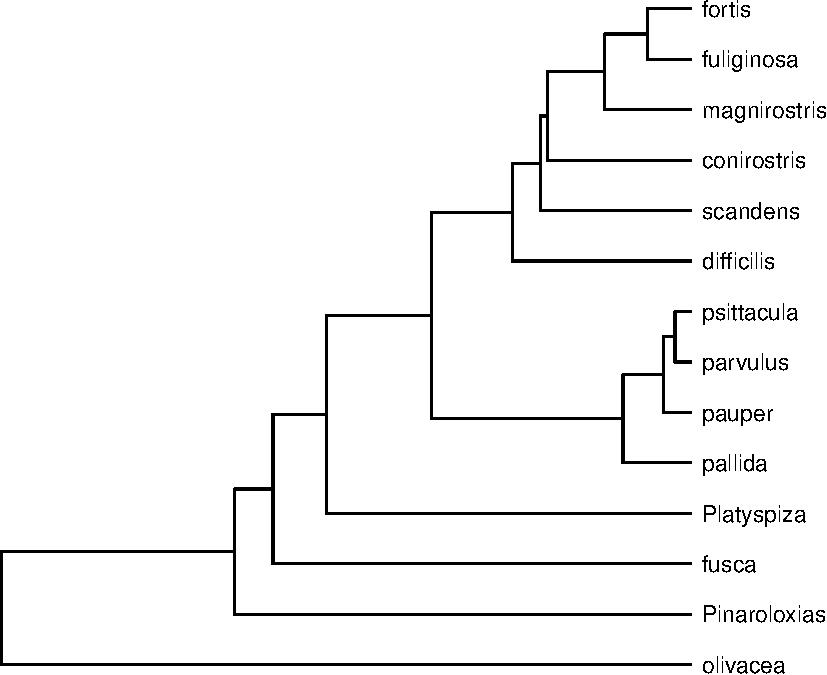
\includegraphics{bookdown-demo_files/figure-latex/unnamed-chunk-65-1} 

}

\caption{Phylogeny of the species contained within the 'geospiza' dataset of the package geiger.}\label{fig:unnamed-chunk-65}
\end{figure}

We need to start by defining the categories for the data. It is likely that you will have already done this in your data frame when using your own data. If so, just make sure the groups are stored as a factor. In this case, we'll just create some random categories to work with for the example.

\begin{Shaded}
\begin{Highlighting}[]
\NormalTok{groups \textless{}{-}}\StringTok{ }\KeywordTok{as.factor}\NormalTok{(}\KeywordTok{c}\NormalTok{(}\KeywordTok{rep}\NormalTok{(}\StringTok{"A"}\NormalTok{, }\DecValTok{4}\NormalTok{), }\KeywordTok{rep}\NormalTok{(}\StringTok{"B"}\NormalTok{, }\DecValTok{5}\NormalTok{), }\KeywordTok{rep}\NormalTok{(}\StringTok{"C"}\NormalTok{, }\DecValTok{4}\NormalTok{)))}
\KeywordTok{names}\NormalTok{(groups) \textless{}{-}}\StringTok{ }\KeywordTok{rownames}\NormalTok{(dat)}
\end{Highlighting}
\end{Shaded}

An important step here (and for every phylogenetic analysis) is making sure the tree and data can be compared. To do this, we should make sure that the rownames of the data are species names and not just numbers. In this case they already are but if they aren't for you data, you can use the following code.

\begin{Shaded}
\begin{Highlighting}[]
\KeywordTok{rownames}\NormalTok{(data) \textless{}{-}}\StringTok{ }\NormalTok{data}\OperatorTok{$}\NormalTok{SPECIES }\CommentTok{\#the column with species names in the data}
\end{Highlighting}
\end{Shaded}

The geiger package has a very useful function called \textbf{name.check} to allow us to check that the rownames of our data match the tip labels of our tree.

\begin{Shaded}
\begin{Highlighting}[]
\KeywordTok{name.check}\NormalTok{(tree, dat)}
\end{Highlighting}
\end{Shaded}

\begin{verbatim}
$tree_not_data
[1] "olivacea"

$data_not_tree
character(0)
\end{verbatim}

We can see that \emph{olivacea} is not in our data. For some analyses, mismatches like this are a problem and you will need to drop the tip from the tree. It actually doesn't matter here because the function we will be using can drop it automatically for us. However, let's see how it's done. Note the use of the function \textbf{drop.tip} from the package \textbf{ape} \citep{ape} which is an essential package to have for this kind of work!

\begin{Shaded}
\begin{Highlighting}[]
\NormalTok{tree \textless{}{-}}\StringTok{ }\NormalTok{ape}\OperatorTok{::}\KeywordTok{drop.tip}\NormalTok{(tree, }\DataTypeTok{tip =} \StringTok{"olivacea"}\NormalTok{)}
\end{Highlighting}
\end{Shaded}

Now we have overwritten the old tree with our pruned tree. Let's check the new one matches the data.

\begin{Shaded}
\begin{Highlighting}[]
\KeywordTok{name.check}\NormalTok{(tree, dat)}
\end{Highlighting}
\end{Shaded}

\begin{verbatim}
[1] "OK"
\end{verbatim}

All that's left now is to run the analysis. First we extract the column of interest from our data and then simply use the function \textbf{aov.phylo}.

\begin{Shaded}
\begin{Highlighting}[]
\NormalTok{d1 \textless{}{-}}\StringTok{ }\NormalTok{dat[,}\DecValTok{1}\NormalTok{]}
\end{Highlighting}
\end{Shaded}

You should notice some similarities and differences from the way you have run ANOVA before. We are still using a formula (the part with \(\sim\)) but not in a separate \textbf{lm} function. We need to specify the tree we want to use (\textbf{tree}) and also how many simulations we want to run. There isn't a firm rule about this but general convention is around 1000 when sampling/bootstrapping/simulations are involved.

\begin{Shaded}
\begin{Highlighting}[]
\NormalTok{x \textless{}{-}}\StringTok{ }\KeywordTok{aov.phylo}\NormalTok{(d1 }\OperatorTok{\textasciitilde{}}\StringTok{ }\NormalTok{groups, }\DataTypeTok{phy =}\NormalTok{ tree, }\DataTypeTok{nsim =} \DecValTok{1000}\NormalTok{)}
\end{Highlighting}
\end{Shaded}

\begin{verbatim}
Analysis of Variance Table

Response: dat
          Df   Sum-Sq  Mean-Sq F-value  Pr(>F) Pr(>F) given phy
group      2 0.063237 0.031619  3.0067 0.09497           0.1908
Residuals 10 0.105161 0.010516                                 
\end{verbatim}

The results table should be very familiar! The only real difference here is that you have been provided with two p-values. The first (\textbf{Pr(\textgreater F)}) is the p-value without accounting for phylogeny and the second (\textbf{Pr(\textgreater F) given phy}) is the value when we account for phylogeny. In both cases, there is no significant difference between groups.

As you can see, accounting for phylogeny \emph{usually} raises the p-value. This shows us that not accounting for phylogeny increases the risk of type I errors (false positives).

\hypertarget{further-info-2}{%
\section{Further info}\label{further-info-2}}

For further information about the phylogenetic ANOVA, you can read the original paper by Garland \emph{et al} \citeyearpar{garland93}.

\hypertarget{asr1}{%
\chapter{Ancestral State Reconstruction I}\label{asr1}}

This chapter will take you through the code we can use to run ancestral state reconstruction with \textbf{categorical} characters. As always, remember to begin by setting your working directory to wherever you have saved the data files.

\hypertarget{data}{%
\section{Data}\label{data}}

The first thing we need to do is load some data. When you're doing this, you need to keep in mind that you should keep your workspace as well organised as possible. In practice, this means giving things good names. ``RicksDataV1.1'' is not a great name depending on how many datasets you want in there. Neither is ``data1'' if you plan on having multiple datasets (which we do). So give your data object, and all other objects, simple, useful names. My personal preference is to use the name of the group but whatever works is fine. You need to be able to keep track of everything.

\begin{Shaded}
\begin{Highlighting}[]
\NormalTok{macaques \textless{}{-}}\StringTok{ }\KeywordTok{read.table}\NormalTok{(}\StringTok{"macaque\_data.txt"}\NormalTok{, }\DataTypeTok{header =} \OtherTok{TRUE}\NormalTok{)}
\end{Highlighting}
\end{Shaded}

In your environment panel there should be a data frame with 16 observations of 2 variables. This command will show us the top 6 rows of data. It's helpful to have a quick look and see R has loaded what we expected. In this case our data contains 15 species of macaque and one species of baboon alongside data regarding whether they exhibit sexual swellings or not (1/0).

\begin{Shaded}
\begin{Highlighting}[]
\KeywordTok{head}\NormalTok{(macaques)}
\end{Highlighting}
\end{Shaded}

\begin{verbatim}
              species swelling
1    Macaca_arctoides        0
2   Macaca_assamensis        0
3     Macaca_cyclopis        1
4 Macaca_fascicularis        1
5      Macaca_fuscata        1
6        Macaca_maura        1
\end{verbatim}

\hypertarget{trees}{%
\section{Trees}\label{trees}}

Now we need to load the tree using the \textbf{read.nexus} function in the package \textbf{ape} \citep{ape}.

\begin{Shaded}
\begin{Highlighting}[]
\NormalTok{macaque.tree \textless{}{-}}\StringTok{ }\KeywordTok{read.nexus}\NormalTok{(}\StringTok{"macaque\_tree.nex"}\NormalTok{)}
\end{Highlighting}
\end{Shaded}

Let's plot the tree to make sure it loaded correctly. I've used base graphics here rather than ggtree (annotated to let you know what it does). Feel free to have a mess around with these options so you get a feel for what they do. The second function ``tiplabels'' adds some extra tip labels containing the data from the second column of our macaque data.

\begin{Shaded}
\begin{Highlighting}[]
\KeywordTok{plot}\NormalTok{(macaque.tree,        }\CommentTok{\#Tree object}
     \DataTypeTok{cex =} \FloatTok{0.7}\NormalTok{,           }\CommentTok{\#Font size for tip labels}
     \DataTypeTok{label.offset =} \FloatTok{0.3}\NormalTok{,  }\CommentTok{\#Create a space between tip and label}
     \DataTypeTok{edge.color =} \StringTok{"blue"}\NormalTok{, }\CommentTok{\#Paint the branches blue}
     \DataTypeTok{edge.width =} \DecValTok{2}\NormalTok{,      }\CommentTok{\#Make the branches thicker}
     \DataTypeTok{no.margin =} \OtherTok{TRUE}\NormalTok{)    }\CommentTok{\#remove blank margins  }
\KeywordTok{tiplabels}\NormalTok{(macaques[,}\DecValTok{2}\NormalTok{], }\DataTypeTok{bg =} \StringTok{"white"}\NormalTok{, }\DataTypeTok{cex =} \FloatTok{0.7}\NormalTok{)}
\end{Highlighting}
\end{Shaded}

\begin{center}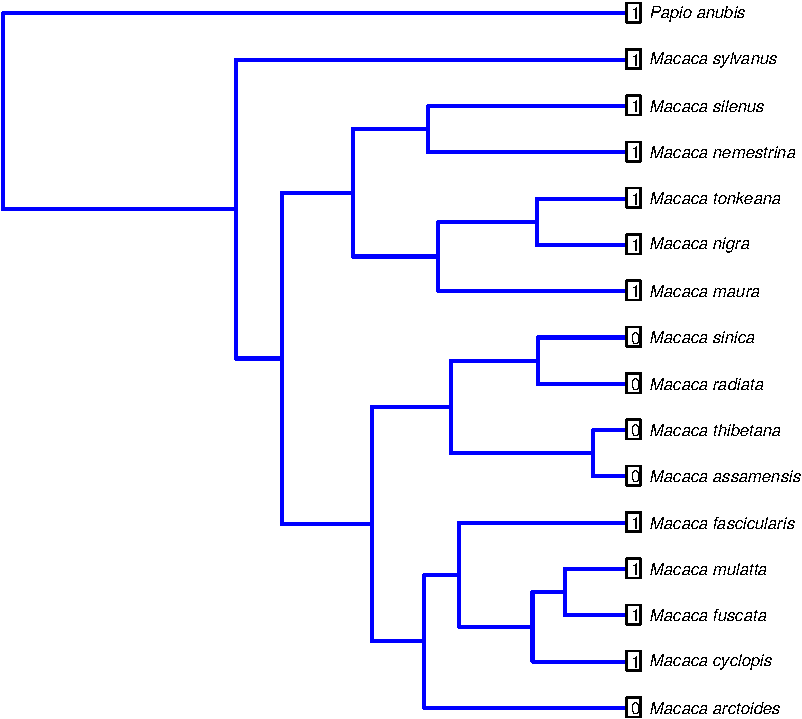
\includegraphics{bookdown-demo_files/figure-latex/unnamed-chunk-79-1} \end{center}

\hypertarget{parsimony}{%
\section{Parsimony}\label{parsimony}}

Let's first generate the most parsimonious reconstruction of the history of this trait. Remember that the most parsimonious history is the one that has the fewest evolutionary transitions. Parsimony is conceptually based upon Occam's razor which states that all else being equal, the simplest explanantion is always the correct one.

The function for this is \textbf{MPR}. It takes an unrooted tree and asks you to specify the root. In our case, we'll have to unroot our tree and then re-root it by specifying that \emph{Papio anubis} is our outgroup.

\begin{Shaded}
\begin{Highlighting}[]
\NormalTok{mp1 \textless{}{-}}\StringTok{ }\KeywordTok{MPR}\NormalTok{(macaques[,}\DecValTok{2}\NormalTok{], }\KeywordTok{unroot}\NormalTok{(macaque.tree), }\StringTok{"Papio\_anubis"}\NormalTok{)}
\end{Highlighting}
\end{Shaded}

When we investigate mp1, we can see a list of results matched up to numbered nodes on the tree. Some nodes are clearly in state 1 and others in state 0. Interestingly some are indeterminate and could be either 0 or 1 such as nodes 19 and 20.

\begin{Shaded}
\begin{Highlighting}[]
\NormalTok{mp1}
\end{Highlighting}
\end{Shaded}

\begin{verbatim}
   lower upper
17     1     1
18     1     1
19     0     1
20     0     1
21     1     1
22     1     1
23     1     1
24     0     0
25     0     0
26     0     0
27     1     1
28     1     1
29     1     1
30     1     1
\end{verbatim}

To get an idea of what this means, we should plot it on the tree. This loop cycles through our results list and combines the lower and upper estimates for each node into a text string that we can then overlay onto that node.

\begin{Shaded}
\begin{Highlighting}[]
\NormalTok{mp.nodes \textless{}{-}}\StringTok{ }\KeywordTok{numeric}\NormalTok{(}\DecValTok{0}\NormalTok{)}
\ControlFlowTok{for}\NormalTok{(i }\ControlFlowTok{in} \DecValTok{1}\OperatorTok{:}\KeywordTok{length}\NormalTok{(mp1[,}\DecValTok{1}\NormalTok{]))\{}
\NormalTok{  mp.nodes \textless{}{-}}\StringTok{ }\KeywordTok{append}\NormalTok{(mp.nodes, }\KeywordTok{paste}\NormalTok{(mp1[i,}\DecValTok{1}\NormalTok{], }\StringTok{","}\NormalTok{, mp1[i,}\DecValTok{2}\NormalTok{]))}
\NormalTok{\}}
\end{Highlighting}
\end{Shaded}

Once we've done that we can plot those expressions onto the tree with the function nodelabels.

\begin{Shaded}
\begin{Highlighting}[]
\KeywordTok{plot}\NormalTok{(macaque.tree, }\DataTypeTok{cex =} \FloatTok{0.7}\NormalTok{, }\DataTypeTok{label.offset =} \FloatTok{0.3}\NormalTok{,}
     \DataTypeTok{edge.color =} \StringTok{"blue"}\NormalTok{, }\DataTypeTok{edge.width =} \DecValTok{2}\NormalTok{, }\DataTypeTok{no.margin =} \OtherTok{TRUE}\NormalTok{)      }
\KeywordTok{tiplabels}\NormalTok{(macaques[,}\DecValTok{2}\NormalTok{], }\DataTypeTok{bg =} \StringTok{"white"}\NormalTok{, }\DataTypeTok{cex =} \FloatTok{0.7}\NormalTok{)}
\KeywordTok{nodelabels}\NormalTok{(mp.nodes, }\KeywordTok{c}\NormalTok{(}\DecValTok{18}\OperatorTok{:}\DecValTok{31}\NormalTok{), }\DataTypeTok{bg =} \StringTok{"white"}\NormalTok{)}
\end{Highlighting}
\end{Shaded}

\begin{center}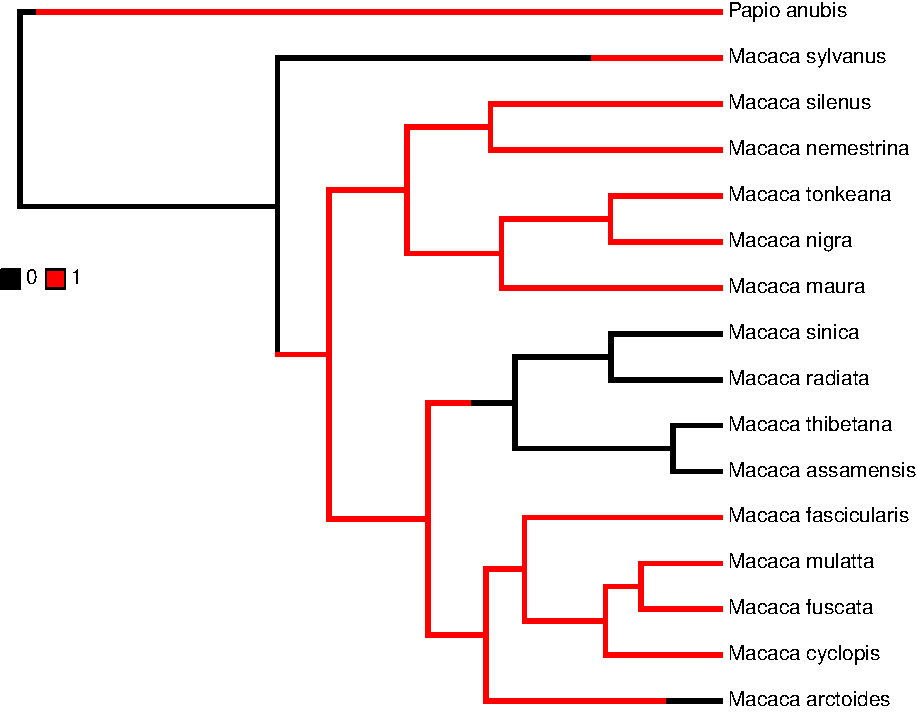
\includegraphics{bookdown-demo_files/figure-latex/unnamed-chunk-83-1} \end{center}

You should note that this isn't a very good plot! There are better ways to represent this information with a little code manipulation. Here's a version using \textbf{ggtree} that plots the character states as points on the tips and the reconstructed nodes.

\begin{figure}[H]

{\centering 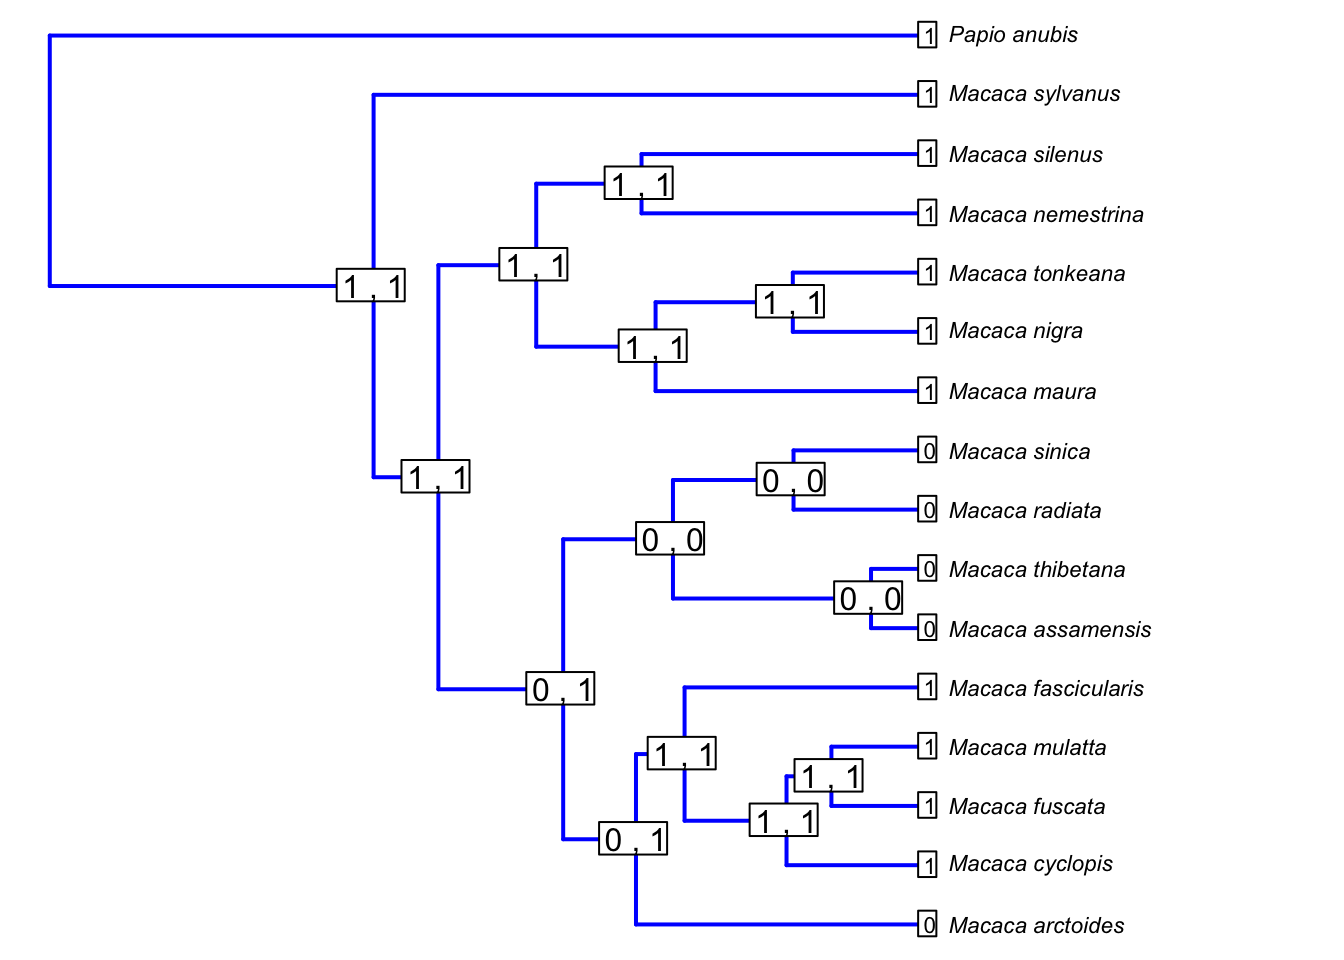
\includegraphics{bookdown-demo_files/figure-latex/unnamed-chunk-84-1} 

}

\caption{Maximum parsimony reconstruction of the evolution of conspicuous sexual swellings in macaques}\label{fig:unnamed-chunk-84}
\end{figure}

As you can see, the uncertainty in some nodes comes from the fact that there seems to be at least two equally parsimonious histories with gains and losses ocurring in different places. For any serious analysis, this is a highly unsatisfactory outcome!

\hypertarget{maximum-likelihood}{%
\section{Maximum Likelihood}\label{maximum-likelihood}}

Let's try a different approach. Maximum likelihood is different from parsimony for many reasons but most significantly, it can make use of branch length information. This is very useful in discriminating between possible histories. A longer branch means more evolutionary change (either in time or character change) and so transitions are more likely to occur on longer branches.

Let's replot the tree. Here I've changed the tiplabels function to plot the character states as colours rather than numbers. The \textbf{bg} argument is what lets me do this. In this argument I list the states (adding 1 because the first is 0) and then the function passes those states to R to assign colours based on a numbered list of standard colours.

\begin{Shaded}
\begin{Highlighting}[]
\KeywordTok{plot}\NormalTok{(macaque.tree, }\DataTypeTok{cex =} \FloatTok{0.7}\NormalTok{, }\DataTypeTok{label.offset =} \FloatTok{0.4}\NormalTok{, }\DataTypeTok{edge.width =} \DecValTok{2}\NormalTok{, }\DataTypeTok{no.margin =} \OtherTok{TRUE}\NormalTok{)}
\KeywordTok{tiplabels}\NormalTok{(}\DataTypeTok{pch =} \DecValTok{21}\NormalTok{, }\DataTypeTok{bg =} \KeywordTok{as.numeric}\NormalTok{(macaques}\OperatorTok{$}\NormalTok{swelling)}\OperatorTok{+}\DecValTok{1}\NormalTok{, }\DataTypeTok{cex =} \FloatTok{1.7}\NormalTok{)}
\end{Highlighting}
\end{Shaded}

\begin{center}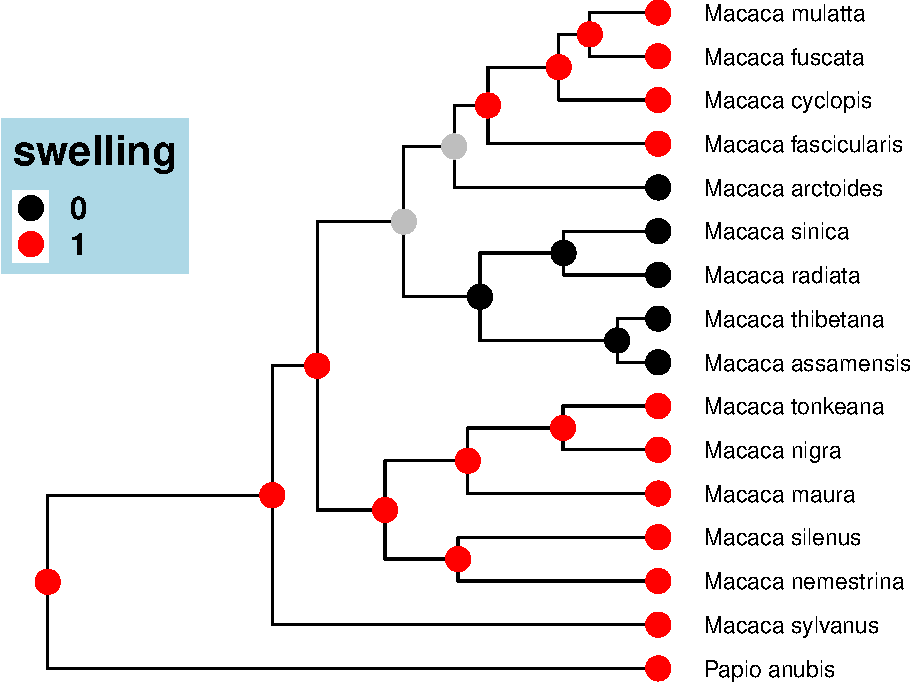
\includegraphics{bookdown-demo_files/figure-latex/unnamed-chunk-85-1} \end{center}

To run an ancestral state reconstruction using maximum likelihood we can use the function \textbf{ace} (ancestral character estimation) in the \textbf{ape} package \citep{ape}. In our first reconstruction, we will make the assumption that the rate of evolution of the trait is equal across the tree by setting the model to \textbf{ER} (equal rates).

\begin{Shaded}
\begin{Highlighting}[]
\NormalTok{m1 \textless{}{-}}\StringTok{ }\KeywordTok{ace}\NormalTok{(}\DataTypeTok{x =}\NormalTok{ macaques}\OperatorTok{$}\NormalTok{swelling,  }\CommentTok{\#trait data}
          \DataTypeTok{phy =}\NormalTok{ macaque.tree,     }\CommentTok{\#phylogeny}
          \DataTypeTok{method =} \StringTok{"ML"}\NormalTok{,          }\CommentTok{\#method (Maximum likelihood)}
          \DataTypeTok{type =} \StringTok{"discrete"}\NormalTok{,      }\CommentTok{\#type of data (continuous or discrete)}
          \DataTypeTok{model =} \StringTok{"ER"}\NormalTok{)           }\CommentTok{\#Model of evolution}
\NormalTok{m1}
\end{Highlighting}
\end{Shaded}

\begin{verbatim}
    Ancestral Character Estimation

Call: ace(x = macaques$swelling, phy = macaque.tree, type = "discrete", 
    method = "ML", model = "ER")

    Log-likelihood: -6.906593 

Rate index matrix:
  0 1
0 . 1
1 1 .

Parameter estimates:
 rate index estimate std-err
          1   0.0319  0.0191

Scaled likelihoods at the root (type '...$lik.anc' to get them for all nodes):
         0          1 
0.08625654 0.91374346 
\end{verbatim}

Looking at the results shows us the likelihood at the root (91\% in favour of state 1 here). However, it's always best to plot the results. We can represent the likelihoods at each node with a piechart. Generally speaking, piecharts are awful but when used in this way, they can actually add useful information to a plot and that's the most important point about plotting any data. In this plot, the piecharts represent the probability that each node exhibited sexual swelling (red) or concealed estrus (black). We can see that the two uncertain nodes from our parsimony analysis are now more certain. Visual inspection shows that these nodes have a greater than 75\% probability of having exhibited sexual swellings.

\begin{Shaded}
\begin{Highlighting}[]
\KeywordTok{plot}\NormalTok{(macaque.tree, }\DataTypeTok{cex =} \FloatTok{0.7}\NormalTok{, }\DataTypeTok{label.offset =} \FloatTok{0.4}\NormalTok{, }\DataTypeTok{edge.width =} \DecValTok{2}\NormalTok{, }\DataTypeTok{no.margin =} \OtherTok{TRUE}\NormalTok{)}
\KeywordTok{tiplabels}\NormalTok{(}\DataTypeTok{pch =} \DecValTok{21}\NormalTok{, }\DataTypeTok{bg =} \KeywordTok{as.numeric}\NormalTok{(macaques}\OperatorTok{$}\NormalTok{swelling)}\OperatorTok{+}\DecValTok{1}\NormalTok{, }\DataTypeTok{cex =} \FloatTok{1.7}\NormalTok{)}
\KeywordTok{nodelabels}\NormalTok{(}\DataTypeTok{pie =}\NormalTok{ m1}\OperatorTok{$}\NormalTok{lik.anc, }\DataTypeTok{piecol =} \KeywordTok{c}\NormalTok{(}\StringTok{"black"}\NormalTok{, }\StringTok{"red"}\NormalTok{), }\DataTypeTok{cex =} \FloatTok{0.8}\NormalTok{)}
\end{Highlighting}
\end{Shaded}

\begin{figure}[H]

{\centering 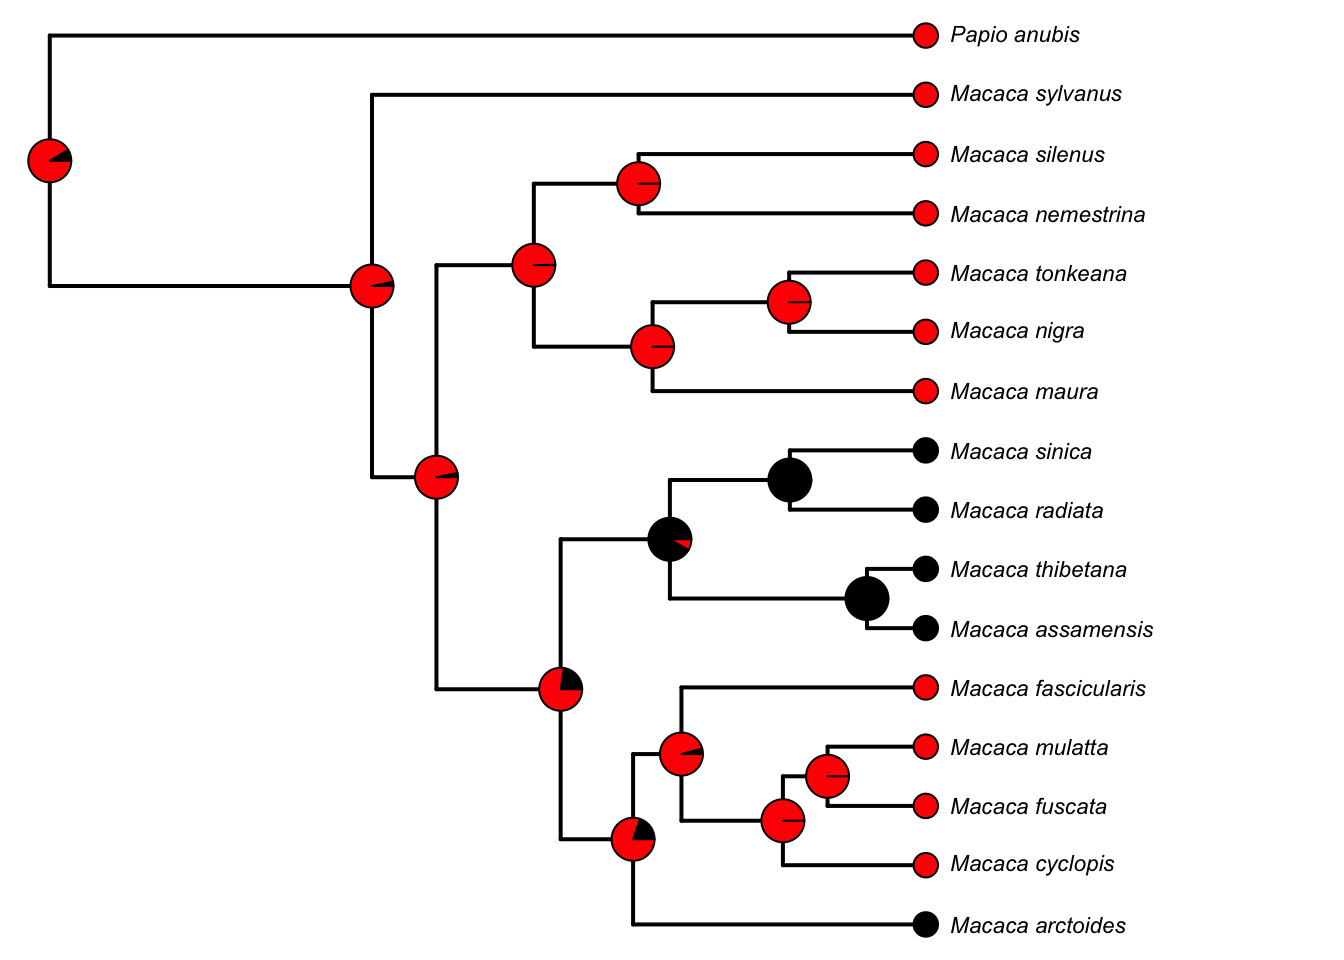
\includegraphics{bookdown-demo_files/figure-latex/unnamed-chunk-87-1} 

}

\caption{Maximum likelihood reconstruction of the evolution of conspicuous sexual swellings in macaques using an equal rates model of evolution.}\label{fig:unnamed-chunk-87}
\end{figure}

Now we can run a similar analysis but let's assume that rates of evolution can vary by setting model to \textbf{ARD} (All Rates Different).

\begin{Shaded}
\begin{Highlighting}[]
\NormalTok{m2 \textless{}{-}}\StringTok{ }\KeywordTok{ace}\NormalTok{(}\DataTypeTok{x =}\NormalTok{ macaques}\OperatorTok{$}\NormalTok{swelling, }\DataTypeTok{phy =}\NormalTok{ macaque.tree,}
          \DataTypeTok{method =} \StringTok{"ML"}\NormalTok{, }\DataTypeTok{type =} \StringTok{"discrete"}\NormalTok{, }\DataTypeTok{model =} \StringTok{"ARD"}\NormalTok{)}

\KeywordTok{plot}\NormalTok{(macaque.tree, }\DataTypeTok{cex =} \FloatTok{0.7}\NormalTok{, }\DataTypeTok{label.offset =} \FloatTok{0.4}\NormalTok{, }\DataTypeTok{edge.width =} \DecValTok{2}\NormalTok{, }\DataTypeTok{no.margin =} \OtherTok{TRUE}\NormalTok{)}
\KeywordTok{tiplabels}\NormalTok{(}\DataTypeTok{pch =} \DecValTok{21}\NormalTok{, }\DataTypeTok{bg =} \KeywordTok{as.numeric}\NormalTok{(macaques}\OperatorTok{$}\NormalTok{swelling)}\OperatorTok{+}\DecValTok{1}\NormalTok{, }\DataTypeTok{cex =} \FloatTok{1.7}\NormalTok{)}
\KeywordTok{nodelabels}\NormalTok{(}\DataTypeTok{pie =}\NormalTok{ m2}\OperatorTok{$}\NormalTok{lik.anc, }\DataTypeTok{piecol =} \KeywordTok{c}\NormalTok{(}\StringTok{"black"}\NormalTok{, }\StringTok{"red"}\NormalTok{), }\DataTypeTok{cex =} \FloatTok{0.8}\NormalTok{)}
\end{Highlighting}
\end{Shaded}

\begin{center}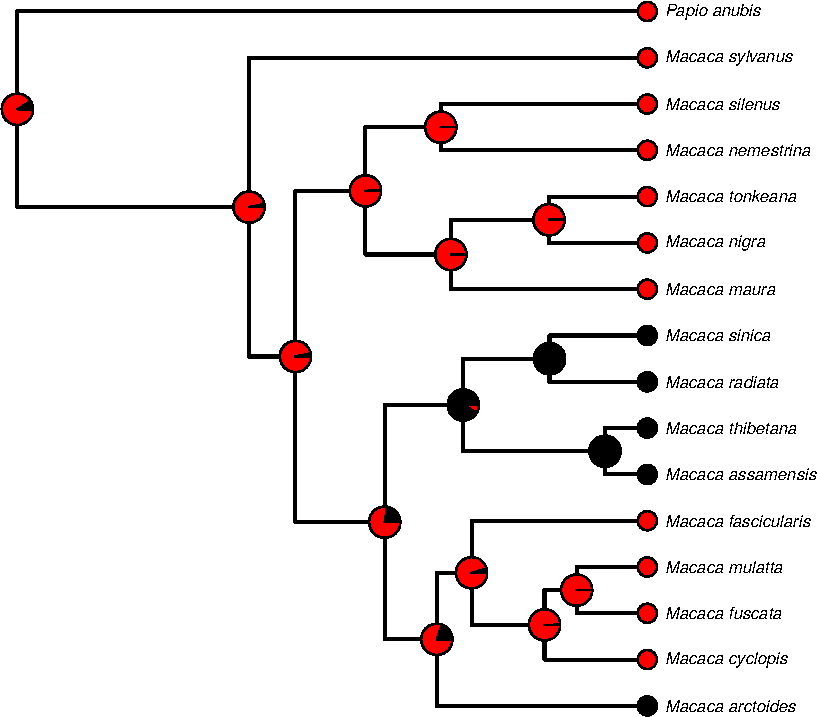
\includegraphics{bookdown-demo_files/figure-latex/unnamed-chunk-88-1} \end{center}

As you can see, the different model of evolution makes a big difference to the results. Which model you choose to use depends on which assumptions you think are justified. Is it fair to assume that the rate of evolution of conspicuous sexual swelling would be constant across the tree as in the equal rates model?

\hypertarget{stochastic-character-mapping}{%
\section{Stochastic Character Mapping}\label{stochastic-character-mapping}}

Stochastic character mapping uses an \textbf{MCMC} (Markov chain Monte-Carlo) approach to sample possible reconstructions from a posterior probability distribution.

Think of the posterior probability distribution as containing all the possible evolutionary histories of the trait in question. This includes some histories in which everything was in one state right up until a few generations from the present when everything swapped around at the same time to give us the distribution we see today. It also contains a history in which the trait switches between 0 and 1 every other generation essentially at random.

Obviously these kind of histories are biologically absurd but not mathematically impossible. They have low statistical probability. Certain other histories will have a high statistical probability and so there will be many similar histories in the distribution. The distribution can be thought of as a histogram with some parameter that defines each particular history.

\hypertarget{an-analogy}{%
\subsection{An Analogy}\label{an-analogy}}

Let's say that we were to plot the entire multiverse as such a distribution using the evil tendencies of one particular occupant (Rick Sanchez) of the multiverse as our parameter. All the different Ricks in all the different universes will vary in their evil tendencies. But overall, Rick's character is actually a nihilist meaning his mean evilness is around 0 when taken over the whole multiverse. Given all this, the posterior distribution of evil Ricks in the multiverse might look like this.

\begin{center}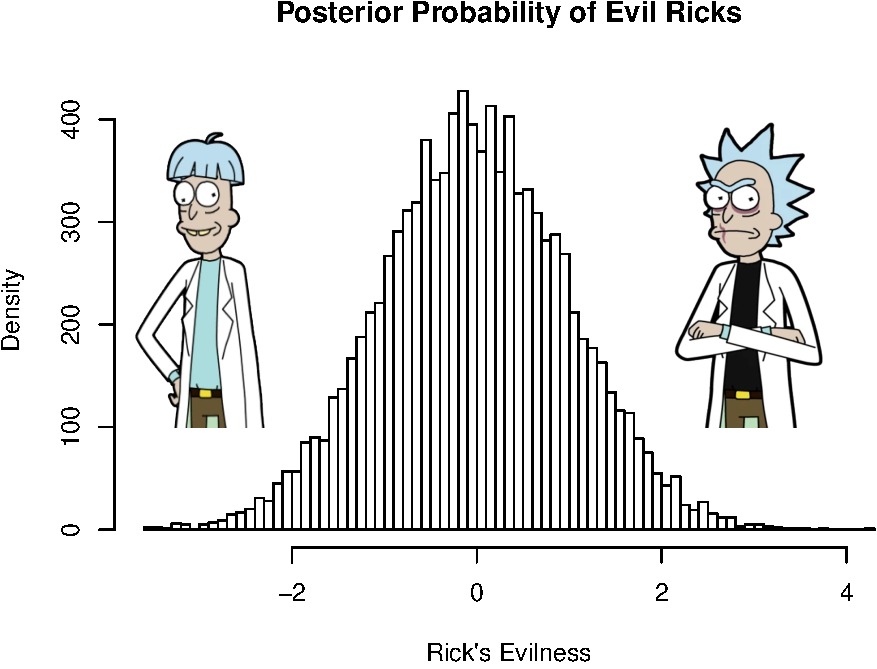
\includegraphics{bookdown-demo_files/figure-latex/unnamed-chunk-89-1} \end{center}

MCMC samples this distribution of histories in a chain. If a history has a higher likelihood than the previous sampling, it is accepted. If it is lower then it is rejected from the sample. In this way, MCMC quickly narrows down the possibilities and gives us a sample of quite likely histories.

\hypertarget{state-characters}{%
\subsection{2-State Characters}\label{state-characters}}

Let's see it in action. We'll need the \textbf{phytools} package \citep{phytools} to create our stochastic character map.

\begin{Shaded}
\begin{Highlighting}[]
\KeywordTok{library}\NormalTok{(phytools)}
\end{Highlighting}
\end{Shaded}

For this analysis (like other phytools functions) we'll need our data in a named vector rather than a data table. Let's call it swelling. The \textbf{names} function attaches the species name to each value in our new vector.

\begin{Shaded}
\begin{Highlighting}[]
\NormalTok{swelling \textless{}{-}}\StringTok{ }\NormalTok{macaques}\OperatorTok{$}\NormalTok{swelling}
\KeywordTok{names}\NormalTok{(swelling) \textless{}{-}}\StringTok{ }\NormalTok{macaques}\OperatorTok{$}\NormalTok{species}
\NormalTok{swelling}
\end{Highlighting}
\end{Shaded}

\begin{verbatim}
   Macaca_arctoides   Macaca_assamensis     Macaca_cyclopis Macaca_fascicularis 
                  0                   0                   1                   1 
     Macaca_fuscata        Macaca_maura      Macaca_mulatta   Macaca_nemestrina 
                  1                   1                   1                   1 
       Macaca_nigra      Macaca_radiata      Macaca_silenus       Macaca_sinica 
                  1                   0                   1                   0 
    Macaca_sylvanus    Macaca_thibetana     Macaca_tonkeana        Papio_anubis 
                  1                   0                   1                   1 
\end{verbatim}

Now we can sample character histories assuming an \emph{equal rates} model of evolution using the \textbf{make.simmap} function.

\begin{Shaded}
\begin{Highlighting}[]
\NormalTok{scm1 \textless{}{-}}\StringTok{ }\KeywordTok{make.simmap}\NormalTok{(macaque.tree, }\DataTypeTok{x =}\NormalTok{ swelling, }\DataTypeTok{model =} \StringTok{"ER"}\NormalTok{)}
\end{Highlighting}
\end{Shaded}

\begin{verbatim}
make.simmap is sampling character histories conditioned on the transition matrix

Q =
            0           1
0 -0.03185011  0.03185011
1  0.03185011 -0.03185011
(estimated using likelihood);
and (mean) root node prior probabilities
pi =
  0   1 
0.5 0.5 
\end{verbatim}

\begin{verbatim}
Done.
\end{verbatim}

Q here is the matrix of transition rates which we have constrained to be equal (\textbf{model = ``ER''}) which explains why the numbers match. As usual with reconstructions, the best thing is to plot them. Here we can use the phytools function \textbf{plotSimmap} to plot the special object we've created. It even has a companion function to add a legend. The first line here assigns colours to the traits.

\begin{Shaded}
\begin{Highlighting}[]
\NormalTok{cols \textless{}{-}}\StringTok{ }\KeywordTok{setNames}\NormalTok{(}\KeywordTok{c}\NormalTok{(}\StringTok{"black"}\NormalTok{, }\StringTok{"red"}\NormalTok{), }\KeywordTok{sort}\NormalTok{(}\KeywordTok{unique}\NormalTok{(swelling)))}
\KeywordTok{plotSimmap}\NormalTok{(scm1, cols, }\DataTypeTok{pts =}\NormalTok{ F, }\DataTypeTok{lwd =} \DecValTok{3}\NormalTok{, }\DataTypeTok{fsize =} \FloatTok{.8}\NormalTok{)}
\KeywordTok{add.simmap.legend}\NormalTok{(}\DataTypeTok{colors =}\NormalTok{ cols, }\DataTypeTok{vertical =}\NormalTok{ F, }\DataTypeTok{prompt =}\NormalTok{ F, }\DataTypeTok{x =} \DecValTok{0}\NormalTok{, }\DataTypeTok{y =} \DecValTok{10}\NormalTok{, }\DataTypeTok{fsize =} \FloatTok{.8}\NormalTok{)}
\end{Highlighting}
\end{Shaded}

\begin{figure}[H]

{\centering 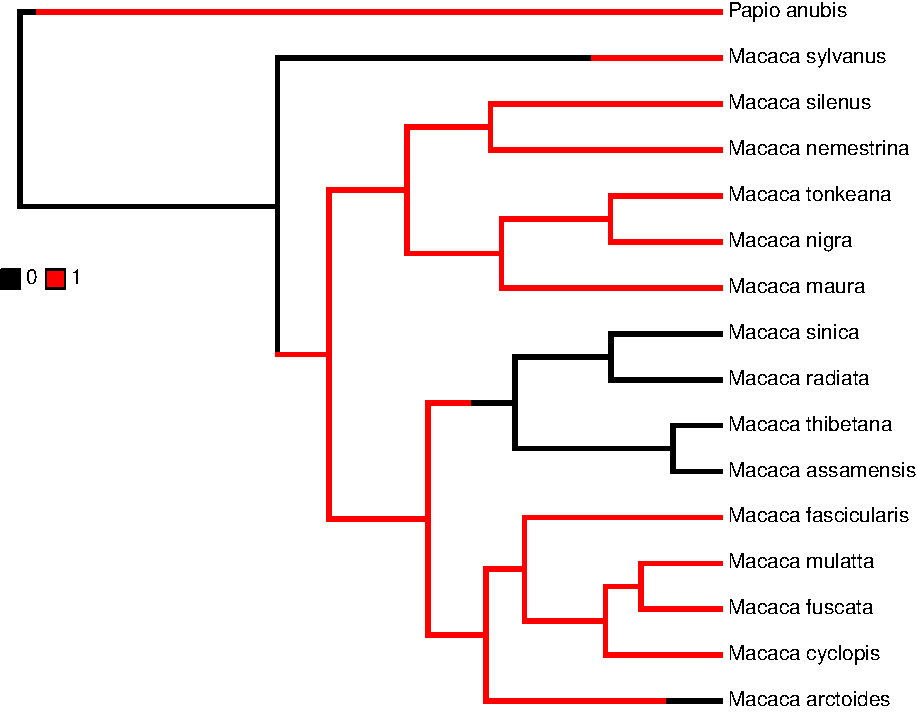
\includegraphics{bookdown-demo_files/figure-latex/unnamed-chunk-94-1} 

}

\caption{Simmap showing a single possible evolutionary history of sexual swelling in macaques.}\label{fig:unnamed-chunk-94}
\end{figure}

Here you can see the single history we have sampled (yours will likely differ). The history contains branches painted according to the trait colour we specified and the position of the transitions on the branch mark the exact position the changes are theorised to have taken place. This is an awful lot of certainty for an ancestral state reconstruction! You should note that the one plotted here is very odd. It says that the ancestor of the group had concealed estrus and then this trait was lost 3 times independently, leaving no trace in the extant species. Given the data and tree we provided, it is hard to see how we can have any confidence in this reconstruction. What evidence have we collected that actually supports this?

However, we need to remember that this only one of the many possible histories! Our next step should be to extract a reasonable sample of these histories!

Let's sample 500 and when R has done that, we can use \textbf{describe.simmap} to summarize the sample.

\begin{Shaded}
\begin{Highlighting}[]
\NormalTok{scm2 \textless{}{-}}\StringTok{ }\KeywordTok{make.simmap}\NormalTok{(macaque.tree, swelling, }\DataTypeTok{model =} \StringTok{"ER"}\NormalTok{, }\DataTypeTok{nsim =} \DecValTok{500}\NormalTok{)}
\end{Highlighting}
\end{Shaded}

\begin{verbatim}
make.simmap is sampling character histories conditioned on the transition matrix

Q =
            0           1
0 -0.03185011  0.03185011
1  0.03185011 -0.03185011
(estimated using likelihood);
and (mean) root node prior probabilities
pi =
  0   1 
0.5 0.5 
\end{verbatim}

\begin{verbatim}
Done.
\end{verbatim}

\begin{Shaded}
\begin{Highlighting}[]
\NormalTok{scm2.sum \textless{}{-}}\StringTok{ }\KeywordTok{describe.simmap}\NormalTok{(scm2, }\DataTypeTok{plot =} \OtherTok{FALSE}\NormalTok{)}
\end{Highlighting}
\end{Shaded}

When we call up the summary, we can see some interesting details about our sample. It seems to be saying that transitions from 1 to 0 (a loss of sexual swelling) happen more frequently than gains of sexual swelling.

\begin{Shaded}
\begin{Highlighting}[]
\NormalTok{scm2.sum}
\end{Highlighting}
\end{Shaded}

\begin{verbatim}
500 trees with a mapped discrete character with states:
 0, 1 

trees have 2.872 changes between states on average

changes are of the following types:
       0,1   1,0
x->y 0.758 2.114

mean total time spent in each state is:
              0          1   total
raw  17.6835904 71.4988096 89.1824
prop  0.1982857  0.8017143  1.0000
\end{verbatim}

As usual, we're going to want a summary plot. The backbone of this plot won't look quite the same as the previous one. You don't want confusing information on your plot so here it would be better to plot a blank backbone (ie a tree with just one colour of branch that doesn't match the colour of the traits) and represent the trait transitions as we did previously with pie charts. In this case the pies represent the proportion of histories in each state (1 or 0) at each node.

\begin{Shaded}
\begin{Highlighting}[]
\NormalTok{cols.null \textless{}{-}}\StringTok{ }\KeywordTok{setNames}\NormalTok{(}\KeywordTok{c}\NormalTok{(}\StringTok{"darkgrey"}\NormalTok{, }\StringTok{"darkgrey"}\NormalTok{), }\KeywordTok{sort}\NormalTok{(}\KeywordTok{unique}\NormalTok{(swelling)))}
\KeywordTok{plotSimmap}\NormalTok{(scm2[[}\DecValTok{1}\NormalTok{]], }\DataTypeTok{lwd =} \DecValTok{3}\NormalTok{, }\DataTypeTok{pts =}\NormalTok{ F, }\DataTypeTok{setEnv =}\NormalTok{ T, }\DataTypeTok{colors =}\NormalTok{ cols.null, }\DataTypeTok{offset =} \FloatTok{.6}\NormalTok{)}
\KeywordTok{nodelabels}\NormalTok{(}\DataTypeTok{pie =}\NormalTok{ scm2.sum}\OperatorTok{$}\NormalTok{ace, }\DataTypeTok{piecol =}\NormalTok{ cols, }\DataTypeTok{cex =} \FloatTok{0.6}\NormalTok{)}
\KeywordTok{add.simmap.legend}\NormalTok{(}\DataTypeTok{colors =}\NormalTok{ cols, }\DataTypeTok{vertical =}\NormalTok{ F, }\DataTypeTok{prompt =}\NormalTok{ F, }\DataTypeTok{x =} \DecValTok{0}\NormalTok{, }\DataTypeTok{y =} \DecValTok{10}\NormalTok{, }\DataTypeTok{fsize =} \FloatTok{.8}\NormalTok{)}
\KeywordTok{tiplabels}\NormalTok{(}\DataTypeTok{pch =} \DecValTok{21}\NormalTok{, }\DataTypeTok{bg =} \KeywordTok{as.numeric}\NormalTok{(macaques}\OperatorTok{$}\NormalTok{swelling)}\OperatorTok{+}\DecValTok{1}\NormalTok{, }\DataTypeTok{cex =} \DecValTok{2}\NormalTok{)}
\end{Highlighting}
\end{Shaded}

\begin{figure}[H]

{\centering 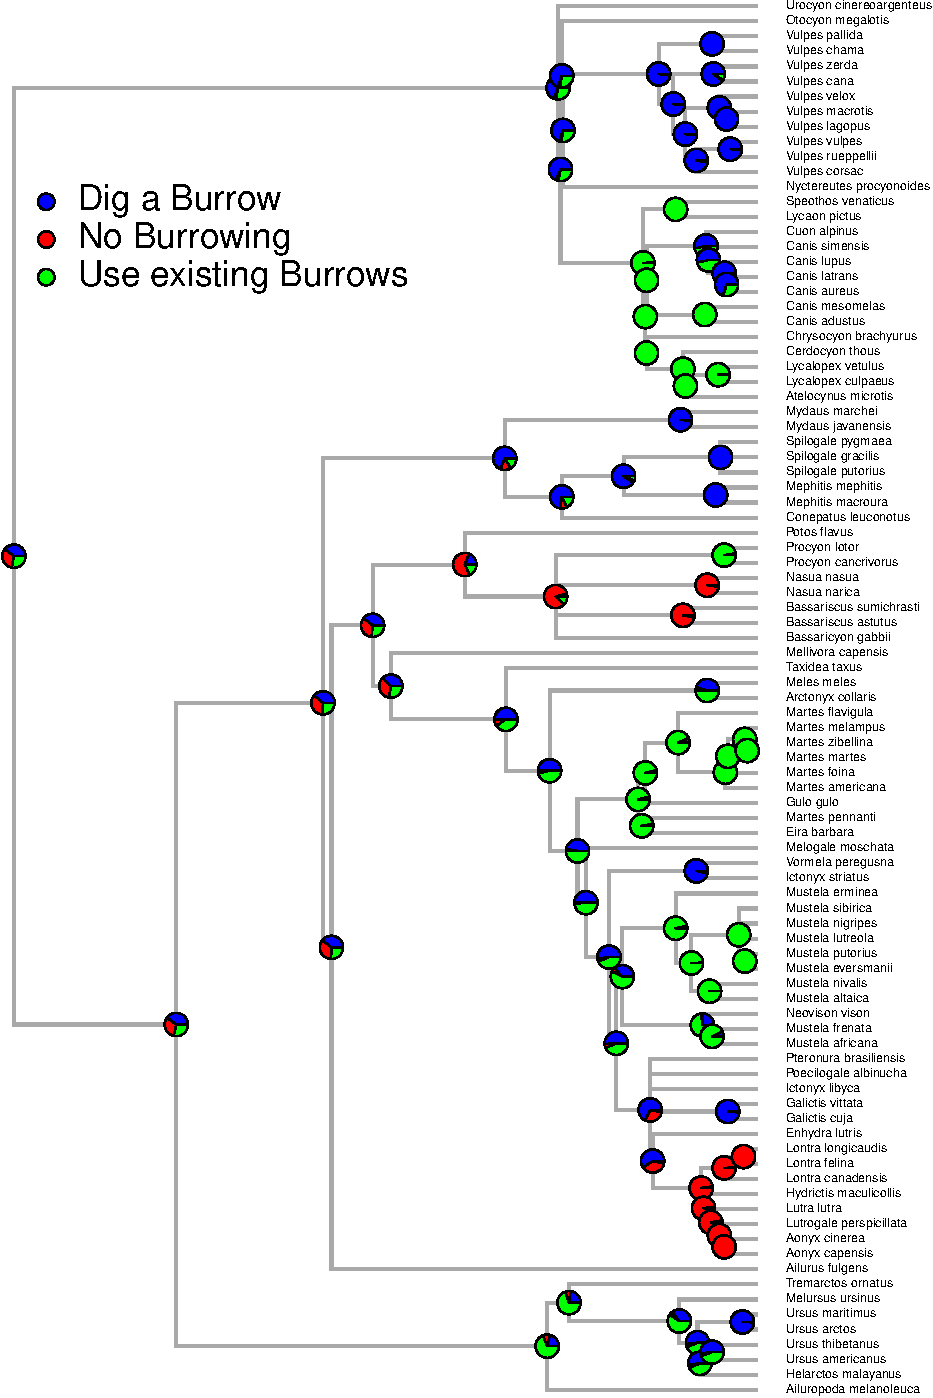
\includegraphics{bookdown-demo_files/figure-latex/unnamed-chunk-97-1} 

}

\caption{Summary of 500 sampled discrete character histories showing the evolution of sexual swellings in macaques.}\label{fig:unnamed-chunk-97}
\end{figure}

This analysis gives us a very similar output to the maximum likelihood analysis in the previous section. If you're intrested, give this analysis another try with different models of evolution.

\hypertarget{state-characters-1}{%
\subsection{3-State Characters}\label{state-characters-1}}

Stochastic character mapping can also be used for traits with more than one state. For example, burrowing in carnivores can be classified as 0 (no burrowing), 1 (use a burrow dug by another animal) or 2 (dig your own burrow).

\hypertarget{data-1}{%
\subsubsection{Data}\label{data-1}}

Let's load some data from a paper which investigated aposematism in terrestrial carnivores \citep{Stankowich11}. Don't forget to assign the species names to rownames to keep everything tidy while we manipulate the data. We also have a tree covering all carnivores \citep{Nyakatura12}.

\begin{Shaded}
\begin{Highlighting}[]
\NormalTok{carn.tree \textless{}{-}}\StringTok{ }\KeywordTok{read.nexus}\NormalTok{(}\StringTok{"carnivores\_tree.nex"}\NormalTok{)}
\NormalTok{carn.data \textless{}{-}}\StringTok{ }\KeywordTok{read.table}\NormalTok{(}\StringTok{"carnivores\_data.txt"}\NormalTok{, }\DataTypeTok{header =}\NormalTok{ T)}
\KeywordTok{rownames}\NormalTok{(carn.data) \textless{}{-}}\StringTok{ }\NormalTok{carn.data}\OperatorTok{$}\NormalTok{Species}
\end{Highlighting}
\end{Shaded}

If you look at the new object \textbf{carn.tree} you'll notice it is a multiPhylo object. This means it actually contains a number of trees rather than just one. For more details about this class of object, see chapter 3.

For now, we just want the first one in the list (based on the best estimates used to date the tree). I'll also prune it a bit to get rid of some of the species I'm not interested in for now.

\begin{Shaded}
\begin{Highlighting}[]
\NormalTok{carn.tree \textless{}{-}}\StringTok{ }\NormalTok{carn.tree[[}\DecValTok{1}\NormalTok{]]}
\NormalTok{carn.tree \textless{}{-}}\StringTok{ }\KeywordTok{extract.clade}\NormalTok{(carn.tree, }\DataTypeTok{node =} \StringTok{"\textquotesingle{}123\textquotesingle{}"}\NormalTok{)}
\end{Highlighting}
\end{Shaded}

Unlike the macaque data from earlier, the carnivore data needs a little more tidying. Now that you're more comfortable using R, you should make this standard practice whenever you load data and a tree for an analysis!

We can use the function \textbf{name.check} in the package \textbf{geiger} to help us out here \citep{geiger}. This function returns two lists. The first contains all the species that appear in the phylogeny but not in the dataset. The second has the species that occur in the data but not in the tree.

\begin{Shaded}
\begin{Highlighting}[]
\NormalTok{geiger}\OperatorTok{::}\KeywordTok{name.check}\NormalTok{(}\DataTypeTok{phy =}\NormalTok{ carn.tree, }\DataTypeTok{data =}\NormalTok{ carn.data)}
\end{Highlighting}
\end{Shaded}

\begin{verbatim}
$tree_not_data
 [1] "Arctocephalus_australis"     "Arctocephalus_forsteri"     
 [3] "Arctocephalus_galapagoensis" "Arctocephalus_gazella"      
 [5] "Arctocephalus_philippii"     "Arctocephalus_pusillus"     
 [7] "Arctocephalus_townsendi"     "Arctocephalus_tropicalis"   
 [9] "Bassaricyon_alleni"          "Bassaricyon_beddardi"       
[11] "Bassaricyon_lasius"          "Bassaricyon_pauli"          
[13] "Callorhinus_ursinus"         "Conepatus_chinga"           
[15] "Conepatus_humboldtii"        "Conepatus_semistriatus"     
[17] "Cystophora_cristata"         "Dusicyon_australis"         
[19] "Erignathus_barbatus"         "Eumetopias_jubatus"         
[21] "Halichoerus_grypus"          "Histriophoca_fasciata"      
[23] "Hydrurga_leptonyx"           "Leptonychotes_weddellii"    
[25] "Lobodon_carcinophaga"        "Lontra_provocax"            
[27] "Lutra_nippon"                "Lutra_sumatrana"            
[29] "Lycalopex_fulvipes"          "Lycalopex_griseus"          
[31] "Lycalopex_gymnocercus"       "Lycalopex_sechurae"         
[33] "Lyncodon_patagonicus"        "Martes_gwatkinsii"          
[35] "Meles_anakuma"               "Meles_leucurus"             
[37] "Melogale_everetti"           "Melogale_orientalis"        
[39] "Melogale_personata"          "Mirounga_angustirostris"    
[41] "Mirounga_leonina"            "Monachus_monachus"          
[43] "Monachus_schauinslandi"      "Monachus_tropicalis"        
[45] "Mustela_felipei"             "Mustela_itatsi"             
[47] "Mustela_kathiah"             "Mustela_lutreolina"         
[49] "Mustela_nudipes"             "Mustela_strigidorsa"        
[51] "Mustela_subpalmata"          "Nasuella_olivacea"          
[53] "Neophoca_cinerea"            "Neovison_macrodon"          
[55] "Odobenus_rosmarus"           "Ommatophoca_rossii"         
[57] "Otaria_flavescens"           "Pagophilus_groenlandicus"   
[59] "Phoca_largha"                "Phoca_vitulina"             
[61] "Phocarctos_hookeri"          "Procyon_pygmaeus"           
[63] "Pusa_caspica"                "Pusa_hispida"               
[65] "Pusa_sibirica"               "Spilogale_angustifrons"     
[67] "Urocyon_littoralis"          "Vulpes_bengalensis"         
[69] "Vulpes_ferrilata"            "Zalophus_californianus"     
[71] "Zalophus_japonicus"          "Zalophus_wollebaeki"        

$data_not_tree
 [1] "Acinonyx_jubatus"             "Arctictis_binturong"         
 [3] "Arctogalidia_trivirgata"      "Atilax_paludinosus"          
 [5] "Bdeogale_crassicauda"         "Caracal_caracal"             
 [7] "Catopuma_temminckii"          "Chrotogale_owstoni"          
 [9] "Civettictis_civetta"          "Crocuta_crocuta"             
[11] "Crossarchus_obscurus"         "Cryptoprocta_ferox"          
[13] "Cynictis_penicillata"         "Cynogale_bennettii"          
[15] "Dologale_dybowskii"           "Eupleres_goudotii"           
[17] "Felis_chaus"                  "Felis_manul"                 
[19] "Felis_margarita"              "Felis_nigripes"              
[21] "Felis_silvestris"             "Fossa_fossana"               
[23] "Galerella_sanguinea"          "Galidia_elegans"             
[25] "Genetta_abyssinica"           "Genetta_angolensis"          
[27] "Genetta_genetta"              "Genetta_servalina"           
[29] "Genetta_thierryi"             "Helogale_parvula"            
[31] "Hemigalus_derbyanus"          "Herpestes_ichneumon"         
[33] "Herpestes_javanicus"          "Herpestes_urva"              
[35] "Hyaena_brunnea"               "Hyaena_hyaena"               
[37] "Ichneumia_albicauda"          "Leopardus_geoffroyi"         
[39] "Leopardus_guigna"             "Leopardus_jacobitus"         
[41] "Leopardus_pardalis"           "Leopardus_wiedii"            
[43] "Leptailurus_serval"           "Liberiictis_kuhni"           
[45] "Lynx_canadensis"              "Lynx_lynx"                   
[47] "Lynx_pardinus"                "Lynx_rufus"                  
[49] "Macrogalidia_musschenbroekii" "Mungos_gambianus"            
[51] "Mungos_mungo"                 "Mungotictis_decemlineata"    
[53] "Nandinia_binotata"            "Neofelis_nebulosa"           
[55] "Paguma_larvata"               "Panthera_leo"                
[57] "Panthera_onca"                "Panthera_pardus"             
[59] "Panthera_tigris"              "Paracynictis_selousi"        
[61] "Paradoxurus_hermaphroditus"   "Paradoxurus_zeylonensis"     
[63] "Pardofelis_marmorata"         "Poiana_richardsonii"         
[65] "Prionailurus_bengalensis"     "Prionailurus_iriomotensis"   
[67] "Prionailurus_rubiginosus"     "Prionodon_linsang"           
[69] "Prionodon_pardicolor"         "Proteles_cristata"           
[71] "Puma_concolor"                "Salanoia_concolor"           
[73] "Suricata_suricatta"           "Uncia_uncia"                 
[75] "Viverra_megaspila"            "Viverra_tangalunga"          
[77] "Viverra_zibetha"              "Viverricula_indica"          
\end{verbatim}

The easiest thing to do first is drop the tips from the tree that we're not interested in. We can pass the whole list to the \textbf{drop.tip} function in \textbf{ape} for this \citep{ape}.

\begin{Shaded}
\begin{Highlighting}[]
\NormalTok{carn.tree \textless{}{-}}\StringTok{ }\KeywordTok{drop.tip}\NormalTok{(carn.tree, geiger}\OperatorTok{::}\KeywordTok{name.check}\NormalTok{(carn.tree, carn.data)}\OperatorTok{$}\NormalTok{tree\_not\_data)}
\NormalTok{geiger}\OperatorTok{::}\KeywordTok{name.check}\NormalTok{(carn.tree, carn.data)}
\end{Highlighting}
\end{Shaded}

\begin{verbatim}
$tree_not_data
character(0)

$data_not_tree
 [1] "Acinonyx_jubatus"             "Arctictis_binturong"         
 [3] "Arctogalidia_trivirgata"      "Atilax_paludinosus"          
 [5] "Bdeogale_crassicauda"         "Caracal_caracal"             
 [7] "Catopuma_temminckii"          "Chrotogale_owstoni"          
 [9] "Civettictis_civetta"          "Crocuta_crocuta"             
[11] "Crossarchus_obscurus"         "Cryptoprocta_ferox"          
[13] "Cynictis_penicillata"         "Cynogale_bennettii"          
[15] "Dologale_dybowskii"           "Eupleres_goudotii"           
[17] "Felis_chaus"                  "Felis_manul"                 
[19] "Felis_margarita"              "Felis_nigripes"              
[21] "Felis_silvestris"             "Fossa_fossana"               
[23] "Galerella_sanguinea"          "Galidia_elegans"             
[25] "Genetta_abyssinica"           "Genetta_angolensis"          
[27] "Genetta_genetta"              "Genetta_servalina"           
[29] "Genetta_thierryi"             "Helogale_parvula"            
[31] "Hemigalus_derbyanus"          "Herpestes_ichneumon"         
[33] "Herpestes_javanicus"          "Herpestes_urva"              
[35] "Hyaena_brunnea"               "Hyaena_hyaena"               
[37] "Ichneumia_albicauda"          "Leopardus_geoffroyi"         
[39] "Leopardus_guigna"             "Leopardus_jacobitus"         
[41] "Leopardus_pardalis"           "Leopardus_wiedii"            
[43] "Leptailurus_serval"           "Liberiictis_kuhni"           
[45] "Lynx_canadensis"              "Lynx_lynx"                   
[47] "Lynx_pardinus"                "Lynx_rufus"                  
[49] "Macrogalidia_musschenbroekii" "Mungos_gambianus"            
[51] "Mungos_mungo"                 "Mungotictis_decemlineata"    
[53] "Nandinia_binotata"            "Neofelis_nebulosa"           
[55] "Paguma_larvata"               "Panthera_leo"                
[57] "Panthera_onca"                "Panthera_pardus"             
[59] "Panthera_tigris"              "Paracynictis_selousi"        
[61] "Paradoxurus_hermaphroditus"   "Paradoxurus_zeylonensis"     
[63] "Pardofelis_marmorata"         "Poiana_richardsonii"         
[65] "Prionailurus_bengalensis"     "Prionailurus_iriomotensis"   
[67] "Prionailurus_rubiginosus"     "Prionodon_linsang"           
[69] "Prionodon_pardicolor"         "Proteles_cristata"           
[71] "Puma_concolor"                "Salanoia_concolor"           
[73] "Suricata_suricatta"           "Uncia_uncia"                 
[75] "Viverra_megaspila"            "Viverra_tangalunga"          
[77] "Viverra_zibetha"              "Viverricula_indica"          
\end{verbatim}

Dropping species from your dataframe is a little more complex (and in truth not always necessary). One way of doing this is to create a \textbf{for loop} that will cycle through the list above and take a subset of the dataframe each time, removing the species in the list as it goes. There are better ways to do this but it might be helpful to become familiar with for loops which are a useful programming tool!

\begin{Shaded}
\begin{Highlighting}[]
\NormalTok{pruned.data \textless{}{-}}\StringTok{ }\NormalTok{carn.data}
\ControlFlowTok{for}\NormalTok{(i }\ControlFlowTok{in} \DecValTok{1}\OperatorTok{:}\KeywordTok{length}\NormalTok{(geiger}\OperatorTok{::}\KeywordTok{name.check}\NormalTok{(carn.tree, carn.data)}\OperatorTok{$}\NormalTok{data\_not\_tree))\{}
\NormalTok{  pruned.data \textless{}{-}}\StringTok{ }\KeywordTok{subset}\NormalTok{(pruned.data, Species}\OperatorTok{!=}\NormalTok{geiger}\OperatorTok{::}\KeywordTok{name.check}\NormalTok{(carn.tree, carn.data)}\OperatorTok{$}\NormalTok{data\_not\_tree[i])}
\NormalTok{\}}
\NormalTok{geiger}\OperatorTok{::}\KeywordTok{name.check}\NormalTok{(carn.tree, pruned.data)}
\end{Highlighting}
\end{Shaded}

\begin{verbatim}
[1] "OK"
\end{verbatim}

Once your tree and data are cleaned up we're ready to go!

\hypertarget{analysis}{%
\subsubsection{Analysis}\label{analysis}}

As before we need to create a named vector for analysis.

\begin{Shaded}
\begin{Highlighting}[]
\NormalTok{burrow\textless{}{-}pruned.data}\OperatorTok{$}\NormalTok{Burrowing}
\KeywordTok{names}\NormalTok{(burrow)\textless{}{-}pruned.data}\OperatorTok{$}\NormalTok{Species}
\end{Highlighting}
\end{Shaded}

Now we can sample a single history and plot it, this time with three colours!

\begin{Shaded}
\begin{Highlighting}[]
\NormalTok{scm3\textless{}{-}}\KeywordTok{make.simmap}\NormalTok{(carn.tree, burrow, }\DataTypeTok{model=}\StringTok{"ER"}\NormalTok{)}
\end{Highlighting}
\end{Shaded}

\begin{verbatim}
make.simmap is sampling character histories conditioned on the transition matrix

Q =
                     Dig a Burrow No Burrowing Use existing Burrows
Dig a Burrow          -0.05640412   0.02820206           0.02820206
No Burrowing           0.02820206  -0.05640412           0.02820206
Use existing Burrows   0.02820206   0.02820206          -0.05640412
(estimated using likelihood);
and (mean) root node prior probabilities
pi =
        Dig a Burrow         No Burrowing Use existing Burrows 
           0.3333333            0.3333333            0.3333333 
\end{verbatim}

\begin{verbatim}
Done.
\end{verbatim}

\begin{Shaded}
\begin{Highlighting}[]
\NormalTok{cols \textless{}{-}}\StringTok{ }\KeywordTok{setNames}\NormalTok{(}\KeywordTok{c}\NormalTok{(}\StringTok{"blue"}\NormalTok{, }\StringTok{"red"}\NormalTok{, }\StringTok{"green"}\NormalTok{), }\KeywordTok{sort}\NormalTok{(}\KeywordTok{unique}\NormalTok{(burrow)))}
\KeywordTok{plotSimmap}\NormalTok{(scm3, cols, }\DataTypeTok{pts =} \OtherTok{FALSE}\NormalTok{, }\DataTypeTok{lwd =} \DecValTok{2}\NormalTok{, }\DataTypeTok{fsize =} \FloatTok{0.5}\NormalTok{)}
\KeywordTok{add.simmap.legend}\NormalTok{(}\DataTypeTok{colors =}\NormalTok{ cols, }\DataTypeTok{vertical =} \OtherTok{TRUE}\NormalTok{, }\DataTypeTok{prompt =} \OtherTok{FALSE}\NormalTok{, }\DataTypeTok{x =} \DecValTok{2}\NormalTok{, }\DataTypeTok{y =} \DecValTok{80}\NormalTok{, }\DataTypeTok{fsize =} \FloatTok{1.4}\NormalTok{, }\DataTypeTok{shape =} \StringTok{"circle"}\NormalTok{)}
\end{Highlighting}
\end{Shaded}

\begin{center}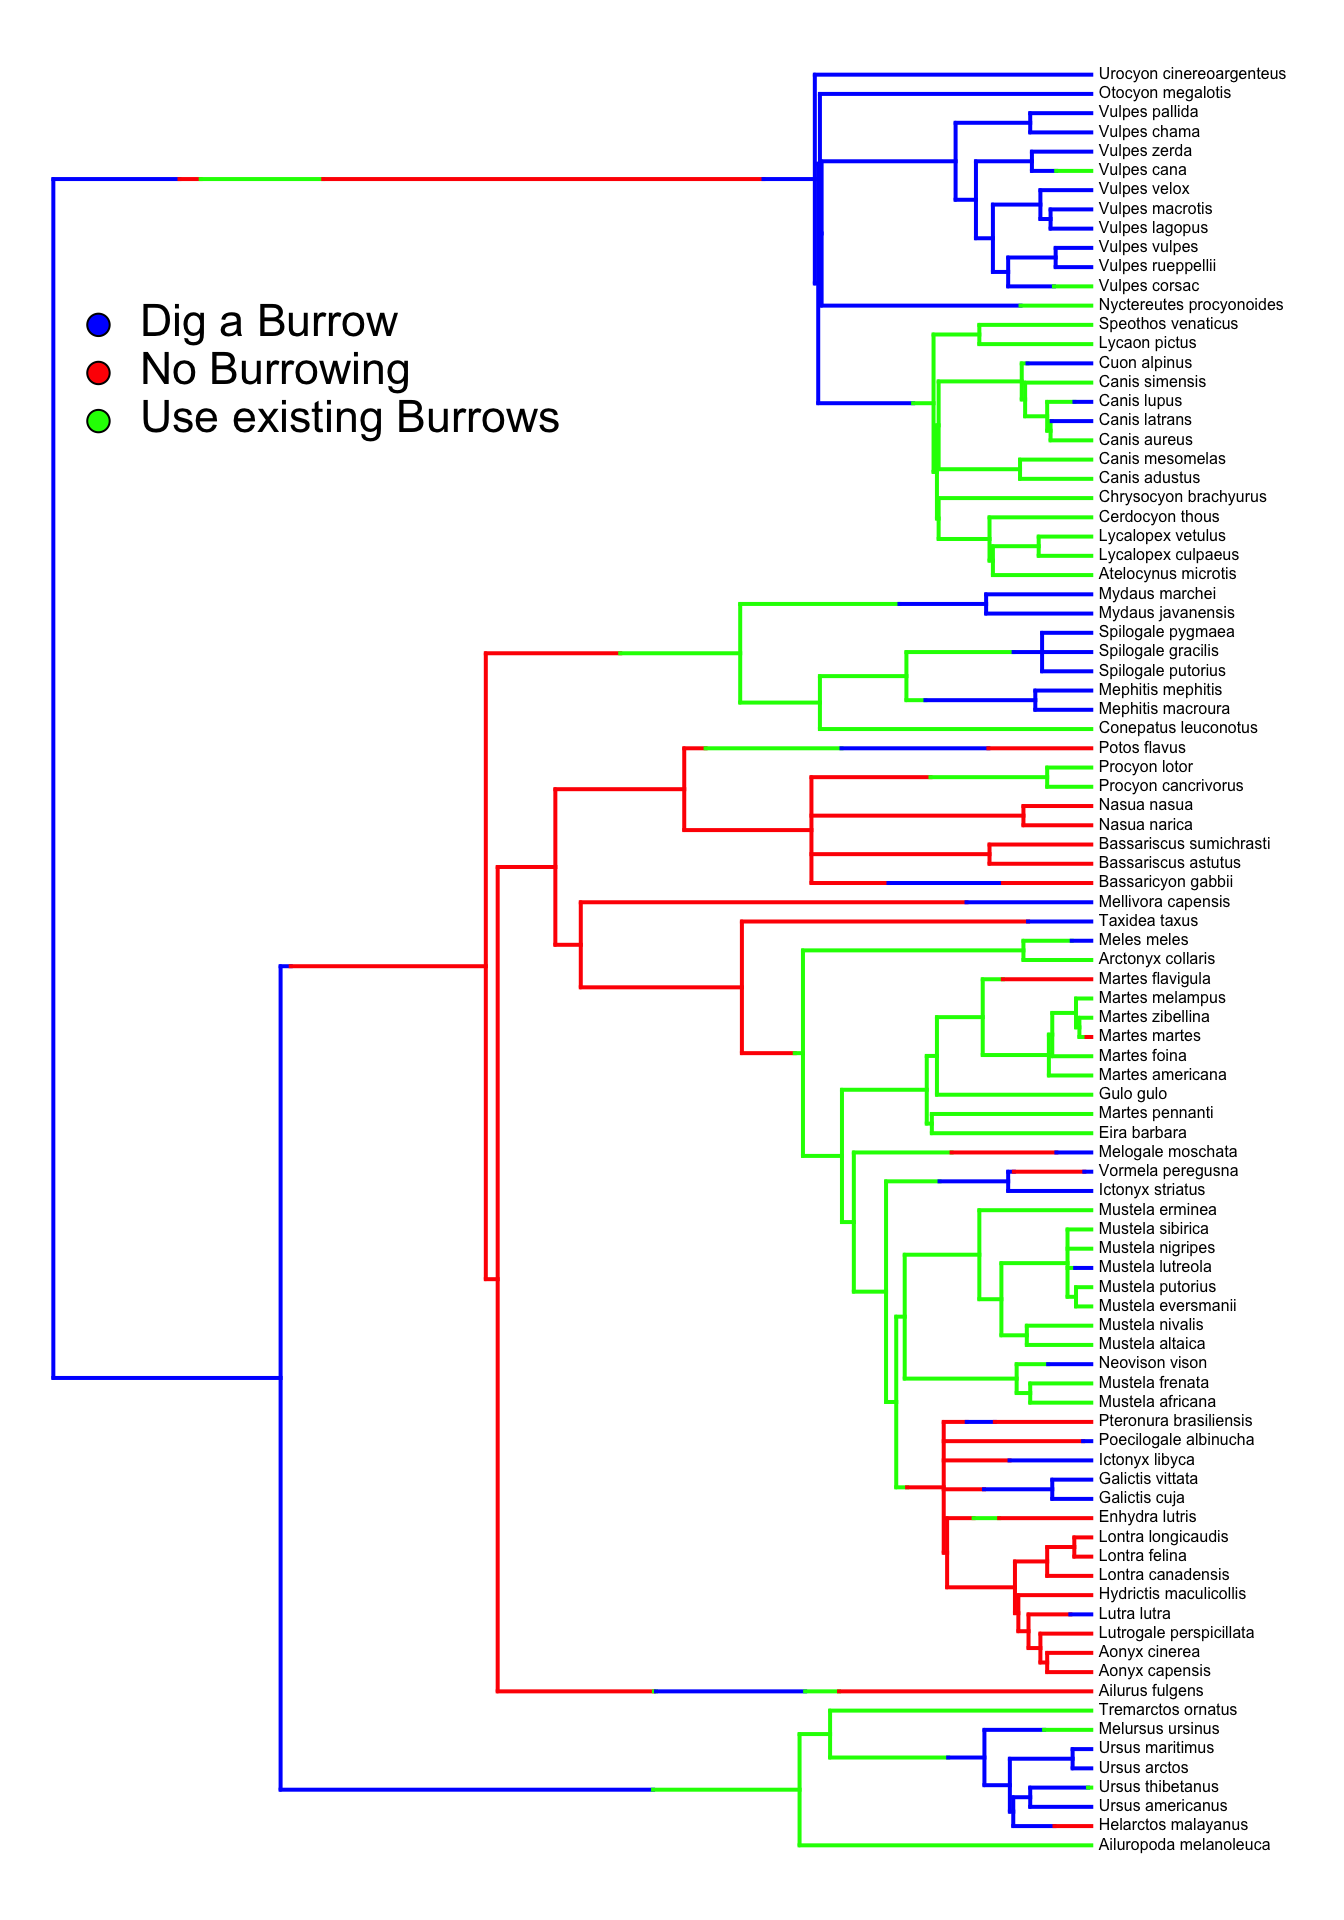
\includegraphics{bookdown-demo_files/figure-latex/unnamed-chunk-106-1} \end{center}

Let's sample 200 possible histories. This may take a few moments. For reports and publications, you should sample more than this. There's no hard rule but 1000 seems to be a good minimum for a proper analysis.

\begin{Shaded}
\begin{Highlighting}[]
\NormalTok{scm4 \textless{}{-}}\StringTok{ }\KeywordTok{make.simmap}\NormalTok{(carn.tree, burrow, }\DataTypeTok{model =} \StringTok{"ER"}\NormalTok{, }\DataTypeTok{nsim =} \DecValTok{200}\NormalTok{)}
\end{Highlighting}
\end{Shaded}

\begin{verbatim}
make.simmap is sampling character histories conditioned on the transition matrix

Q =
                     Dig a Burrow No Burrowing Use existing Burrows
Dig a Burrow          -0.05640412   0.02820206           0.02820206
No Burrowing           0.02820206  -0.05640412           0.02820206
Use existing Burrows   0.02820206   0.02820206          -0.05640412
(estimated using likelihood);
and (mean) root node prior probabilities
pi =
        Dig a Burrow         No Burrowing Use existing Burrows 
           0.3333333            0.3333333            0.3333333 
\end{verbatim}

\begin{verbatim}
Done.
\end{verbatim}

\begin{Shaded}
\begin{Highlighting}[]
\NormalTok{scm4.sum\textless{}{-}}\KeywordTok{describe.simmap}\NormalTok{(scm4, }\DataTypeTok{plot =} \OtherTok{FALSE}\NormalTok{)}
\NormalTok{scm4.sum}
\end{Highlighting}
\end{Shaded}

\begin{verbatim}
200 trees with a mapped discrete character with states:
 Dig a Burrow, No Burrowing, Use existing Burrows 

trees have 52 changes between states on average

changes are of the following types:
     Dig a Burrow,No Burrowing Dig a Burrow,Use existing Burrows
x->y                      7.26                             12.24
     No Burrowing,Dig a Burrow No Burrowing,Use existing Burrows
x->y                     6.925                              5.99
     Use existing Burrows,Dig a Burrow Use existing Burrows,No Burrowing
x->y                            12.265                              7.32

mean total time spent in each state is:
     Dig a Burrow No Burrowing Use existing Burrows total
raw   366.1971509  214.5972284          350.2056207   931
prop    0.3933374    0.2305019            0.3761607     1
\end{verbatim}

Finally we can plot the summary of the analysis as before.

\begin{center}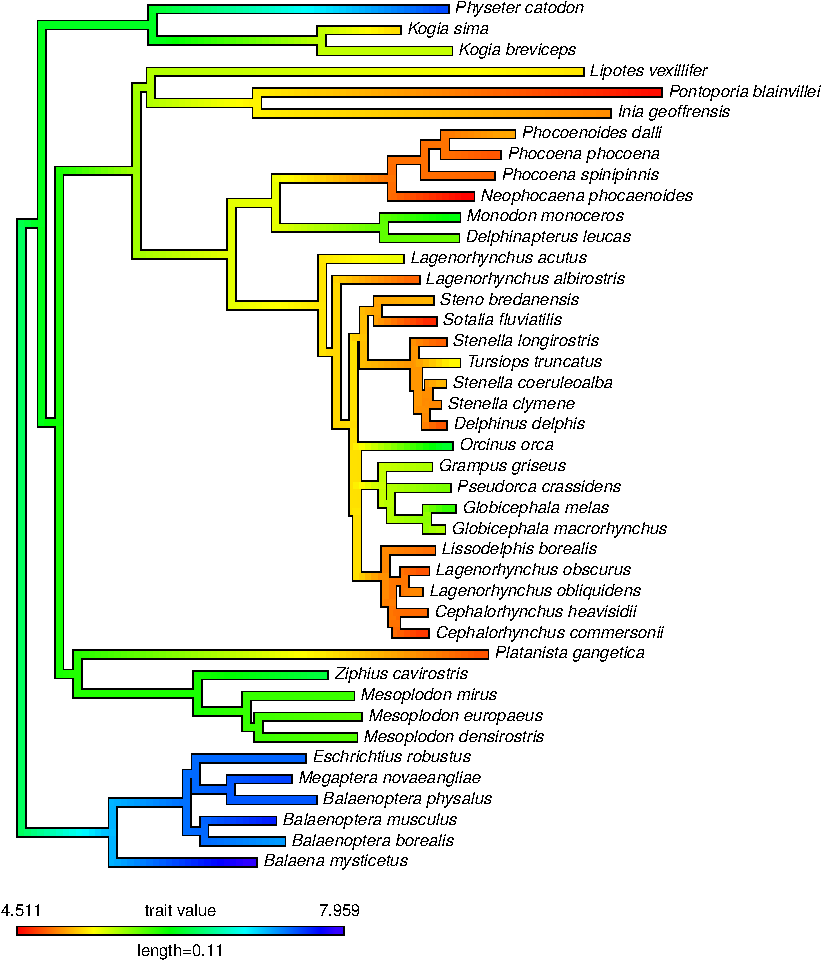
\includegraphics{bookdown-demo_files/figure-latex/unnamed-chunk-108-1} \end{center}

\hypertarget{further-info-3}{%
\section{Further info}\label{further-info-3}}

For more information about ancestral state reconstruction check out a review of the method by Joy \emph{et al}. \citep{Joy16} and chapter 3 of \emph{The comparative approach in evolutionary anthropology and biology} \citep{Nunn11}.

For more information about the phytools package \citep{phytools}, the package author Liam Revell maintains an excellent blog \href{http://blog.phytools.org/}{here} where you'll find lots of useful tips and demonstrations of the package's capabilities as well as some helpful troubleshooting.

\hypertarget{asr2}{%
\chapter{Ancestral State Reconstruction II}\label{asr2}}

Previously, we looked at reconstructing the evolutionary history of binary traits, such as the presence or absence of sexual swellings in macaques, and categorical traits such as the modes of burrowing in carnivores. In this chapter, we'll be applying the same principles to continuous data.

The logic of ancestral state reconstruction applies equally to continuous traits like body size as it does to categorical traits. Here, we'll be looking at the evolutionary history of whales, dolphins and porpoises (Cetacea).

As always, check that you have set your working directory!

\hypertarget{data-2}{%
\section{Data}\label{data-2}}

The data we have here is taken from a study of the evolution of cetacean brain and body size \citep{Montgomery13}. The reduced version here contains only body mass and the log transformed body mass for 42 species.

\begin{Shaded}
\begin{Highlighting}[]
\NormalTok{whale.data \textless{}{-}}\StringTok{ }\KeywordTok{read.table}\NormalTok{(}\StringTok{"whales\_data.txt"}\NormalTok{, }\DataTypeTok{header =}\NormalTok{ T)}
\KeywordTok{rownames}\NormalTok{(whale.data) \textless{}{-}}\StringTok{ }\NormalTok{whale.data}\OperatorTok{$}\NormalTok{species}
\end{Highlighting}
\end{Shaded}

\hypertarget{tree}{%
\section{Tree}\label{tree}}

We also have a tree from the \href{https://10ktrees.nunn-lab.org/}{10ktrees} project \citep{Arnold10}. For more information about this website, see chapter 3.

\begin{Shaded}
\begin{Highlighting}[]
\NormalTok{whale.tree \textless{}{-}}\StringTok{ }\KeywordTok{read.nexus}\NormalTok{(}\StringTok{"whales\_tree.nex"}\NormalTok{)}
\end{Highlighting}
\end{Shaded}

We need to check the data and tree match up. Get into this habit! It will save you a lot of time and patience.

\begin{Shaded}
\begin{Highlighting}[]
\KeywordTok{rownames}\NormalTok{(whale.data) \textless{}{-}}\StringTok{ }\NormalTok{whale.data}\OperatorTok{$}\NormalTok{species}
\NormalTok{geiger}\OperatorTok{::}\KeywordTok{name.check}\NormalTok{(whale.tree, whale.data)}
\end{Highlighting}
\end{Shaded}

\begin{verbatim}
$tree_not_data
 [1] "Balaenoptera_acutorostrata" "Balaenoptera_bonaerensis"  
 [3] "Balaenoptera_edeni"         "Berardius_arnuxii"         
 [5] "Berardius_bairdii"          "Caperea_marginata"         
 [7] "Cephalorhynchus_eutropia"   "Cephalorhynchus_hectori"   
 [9] "Delphinus_capensis"         "Delphinus_tropicalis"      
[11] "Eubalaena_australis"        "Eubalaena_glacialis"       
[13] "Eubalaena_japonica"         "Feresa_attenuata"          
[15] "Hyperoodon_ampullatus"      "Hyperoodon_planifrons"     
[17] "Indopacetus_pacificus"      "Lagenodelphis_hosei"       
[19] "Lagenorhynchus_australis"   "Lagenorhynchus_cruciger"   
[21] "Lissodelphis_peronii"       "Mesoplodon_bidens"         
[23] "Mesoplodon_bowdoini"        "Mesoplodon_carlhubbsi"     
[25] "Mesoplodon_ginkgodens"      "Mesoplodon_grayi"          
[27] "Mesoplodon_hectori"         "Mesoplodon_layardii"       
[29] "Mesoplodon_perrini"         "Mesoplodon_peruvianus"     
[31] "Mesoplodon_stejnegeri"      "Orcaella_brevirostris"     
[33] "Orcaella_heinsohni"         "Peponocephala_electra"     
[35] "Phocoena_dioptrica"         "Phocoena_sinus"            
[37] "Platanista_minor"           "Sousa_chinensis"           
[39] "Stenella_attenuata"         "Stenella_frontalis"        
[41] "Tasmacetus_shepherdi"       "Tursiops_aduncus"          

$data_not_tree
character(0)
\end{verbatim}

Clearly some species need to be dropped from the tree!

\begin{Shaded}
\begin{Highlighting}[]
\NormalTok{whale.tree \textless{}{-}}\StringTok{ }\KeywordTok{drop.tip}\NormalTok{(whale.tree, }
\NormalTok{                       geiger}\OperatorTok{::}\KeywordTok{name.check}\NormalTok{(whale.tree, whale.data)}\OperatorTok{$}\NormalTok{tree\_not\_data)}
\NormalTok{geiger}\OperatorTok{::}\KeywordTok{name.check}\NormalTok{(whale.tree, whale.data)}
\end{Highlighting}
\end{Shaded}

\begin{verbatim}
[1] "OK"
\end{verbatim}

\hypertarget{ancestral-state-reconstructions}{%
\section{Ancestral State Reconstructions}\label{ancestral-state-reconstructions}}

Now we're going to dive in with a reconstruction. We are using \textbf{phytools} for this analysis so we should load the package and create a named data vector \citep{phytools}.

\begin{Shaded}
\begin{Highlighting}[]
\KeywordTok{require}\NormalTok{(phytools)}
\NormalTok{x \textless{}{-}}\StringTok{ }\NormalTok{whale.data}\OperatorTok{$}\NormalTok{log.body.mass}
\KeywordTok{names}\NormalTok{(x) \textless{}{-}}\StringTok{ }\NormalTok{whale.data}\OperatorTok{$}\NormalTok{species}
\end{Highlighting}
\end{Shaded}

The function we need is called \textbf{fastAnc} and it returns the ancestral states in a simple list.

\begin{Shaded}
\begin{Highlighting}[]
\NormalTok{ancstates \textless{}{-}}\StringTok{ }\KeywordTok{fastAnc}\NormalTok{(}\DataTypeTok{tree =}\NormalTok{ whale.tree,   }\CommentTok{\#Our phylogeny}
\NormalTok{                     x,                   }\CommentTok{\#Our data vector}
                     \DataTypeTok{CI =} \OtherTok{TRUE}\NormalTok{)           }\CommentTok{\#Estimate 95\% confidence intervals}
\NormalTok{ancstates}
\end{Highlighting}
\end{Shaded}

\begin{verbatim}
Ancestral character estimates using fastAnc:
      43       44       45       46       47       48       49       50 
6.422936 7.205471 7.440591 7.465284 7.456463 7.511707 6.248774 6.097254 
      51       52       53       54       55       56       57       58 
6.044864 6.078069 5.983733 5.962172 5.641527 5.423179 5.255812 5.204571 
      59       60       61       62       63       64       65       66 
5.225028 5.260263 4.960018 4.901903 4.871755 4.888973 5.503471 5.567067 
      67       68       69       70       71       72       73       74 
5.710190 5.130854 4.989830 5.001555 4.960103 4.976035 5.039423 5.403331 
      75       76       77       78       79       80       81       82 
5.850745 4.870560 4.871380 4.883752 5.590679 5.292187 6.267476 5.540614 

Lower & upper 95% CIs:
      lower    upper
43 5.745860 7.100012
44 6.599516 7.811426
45 7.009526 7.871657
46 7.037792 7.892775
47 7.023487 7.889440
48 7.078101 7.945312
49 5.617637 6.879912
50 5.480639 6.713870
51 5.396996 6.692732
52 5.495449 6.660689
53 5.489021 6.478445
54 5.474786 6.449558
55 4.977189 6.305864
56 4.818460 6.027899
57 4.833079 5.678546
58 4.834286 5.574857
59 4.930739 5.519317
60 4.970172 5.550353
61 4.679687 5.240349
62 4.656292 5.147513
63 4.621817 5.121692
64 4.661301 5.116645
65 5.175817 5.831126
66 5.231290 5.902844
67 5.455762 5.964619
68 4.810518 5.451190
69 4.731256 5.248405
70 4.760819 5.242292
71 4.767162 5.153044
72 4.800446 5.151624
73 4.692067 5.386779
74 4.792073 6.014589
75 5.352644 6.348847
76 4.380205 5.360915
77 4.449659 5.293101
78 4.482168 5.285335
79 4.892863 6.288496
80 4.417990 6.166384
81 5.492347 7.042604
82 4.959783 6.121445
\end{verbatim}

To get an idea of what these results show, we should probably plot it. The \textbf{nodelabels} function maps the ancestral states listed in our \textbf{ancstates} object onto the nodes of the tree which are listed in the same order.

\begin{Shaded}
\begin{Highlighting}[]
\KeywordTok{plot}\NormalTok{(whale.tree, }\DataTypeTok{cex =} \FloatTok{.8}\NormalTok{, }\DataTypeTok{label.offset =} \FloatTok{.01}\NormalTok{, }\DataTypeTok{no.margin =} \OtherTok{TRUE}\NormalTok{)}
\KeywordTok{nodelabels}\NormalTok{(}\KeywordTok{round}\NormalTok{(ancstates}\OperatorTok{$}\NormalTok{ace, }\DataTypeTok{digits =} \DecValTok{2}\NormalTok{), }\DataTypeTok{cex =} \FloatTok{.67}\NormalTok{)}
\end{Highlighting}
\end{Shaded}

\begin{center}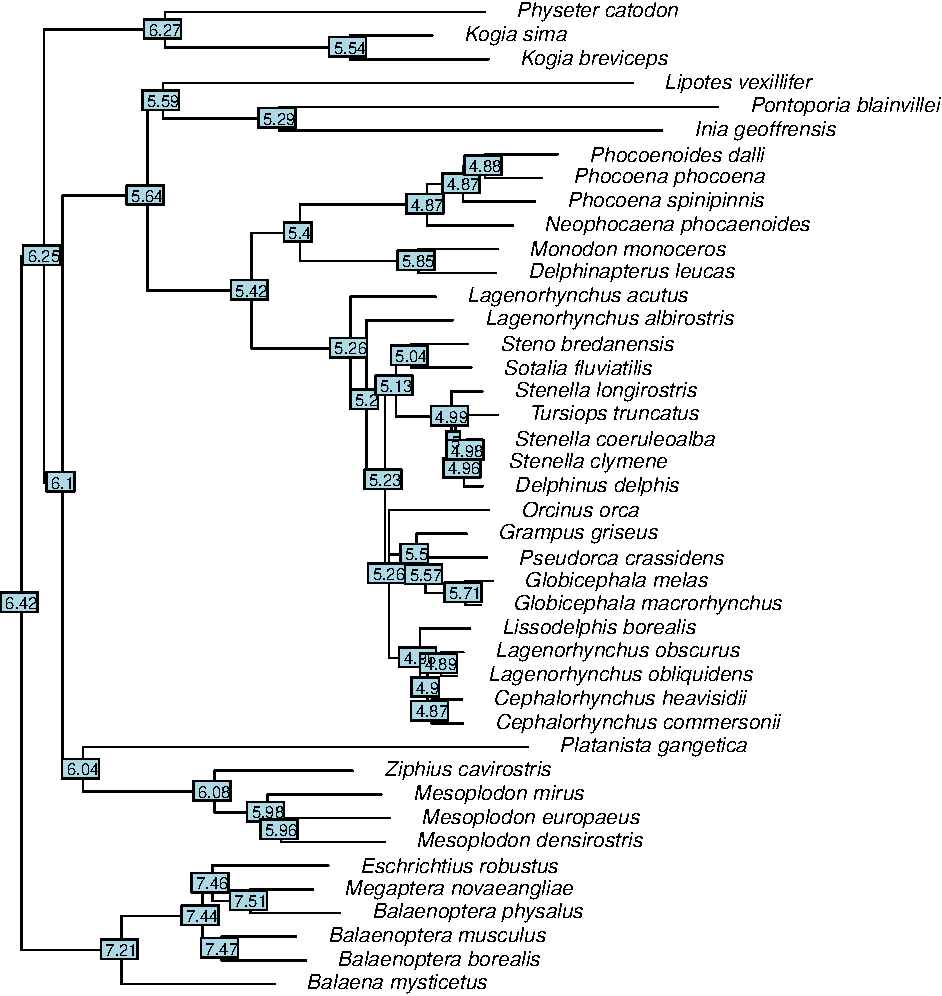
\includegraphics{bookdown-demo_files/figure-latex/unnamed-chunk-118-1} \end{center}

As is often the case, there are better ways to plot this information! The function \textbf{contMap} calls \textbf{fastAnc} and then maps the history of the trait onto the tree as a heatmap. This is a much clearer plot.

\begin{Shaded}
\begin{Highlighting}[]
\KeywordTok{contMap}\NormalTok{(whale.tree, x, }\DataTypeTok{fsize =} \FloatTok{.7}\NormalTok{)}
\end{Highlighting}
\end{Shaded}

\begin{center}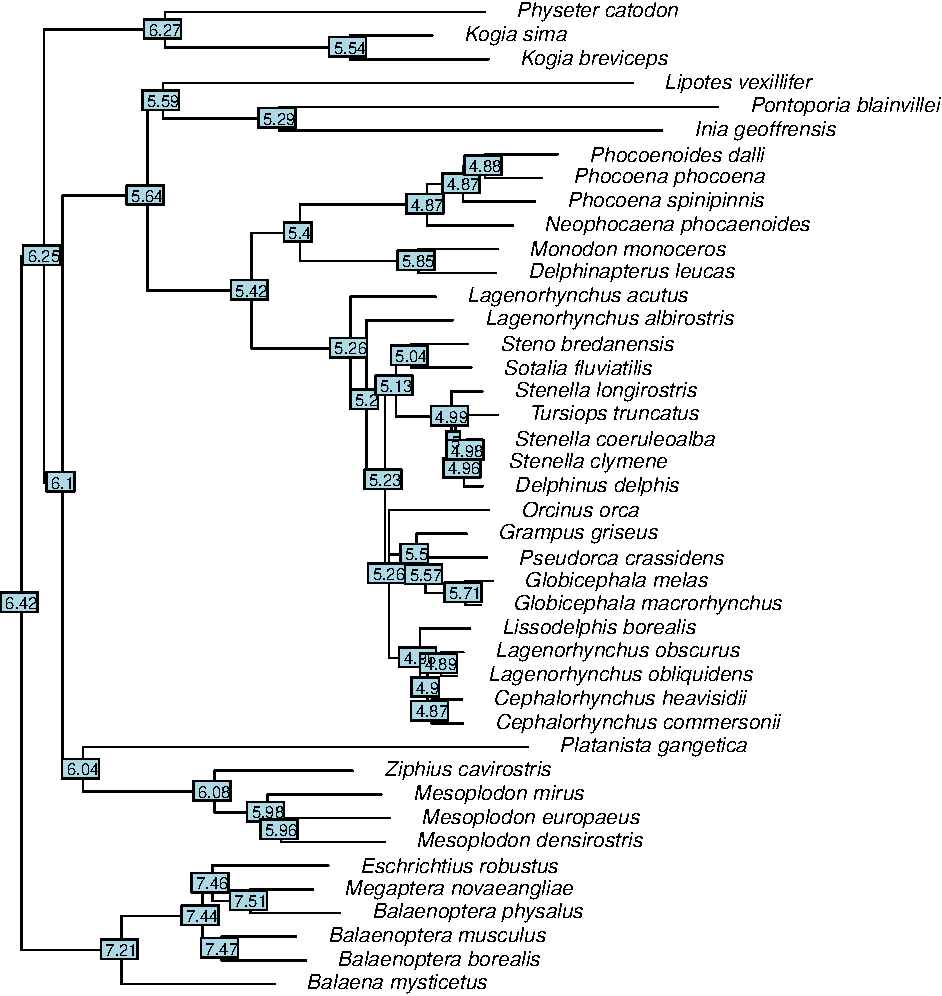
\includegraphics{bookdown-demo_files/figure-latex/unnamed-chunk-119-1} \end{center}

\hypertarget{bayestraits}{%
\section{BayesTraits}\label{bayestraits}}

Simply reconstructing the history of a trait can be very interesting. See some papers by Montgomery \emph{et al}. \citetext{\citeyear{Montgomery10}; \citeyear{Montgomery13}} for just a few great examples. However, this methodology is not limited to simply estimating the past.

Most of what we are going to do here could probably be acheived in R either with existing packages or some clever coding. However, the standard package for several analyses has been \href{http://www.evolution.rdg.ac.uk/BayesTraitsV3.0.2/BayesTraitsV3.0.2.html}{BayesTraits} for some time.

BayesTraits is a command line program, which can make it kind of intimidating. Actually (like R), it's relatively easy to use but can take some getting used to. Fortunately, \href{https://www.randigriffin.com/}{Randi Griffin} has written an excellent R package \textbf{btw} that can operate the program from within R.

It's worth noting at this point that \textbf{btw} is not written to run BayesTraits for you so that you don't have to understand the program. Randi states very clearly that the package is purely for optimising workflow. In other words, this allows you to have all your data, results and code in one place. You still need to understand how to use the program. Fortunately the \href{http://www.evolution.rdg.ac.uk/BayesTraitsV3.0.2/Files/BayesTraitsV3.0.2Manual.pdf}{manual} is very detailed.

First up, download \href{http://www.evolution.rdg.ac.uk/BayesTraitsV3.0.2/BayesTraitsV3.0.2.html}{BayesTraits} version 3 for your operating system.

\textbf{IMPORTANT!} BayesTraits output files will be written into your working directory. They will overwrite any files with the same name so don't have any files called ``data.txt'', ``tree.nex'' or ``inputfile.txt'' in this directory unless you are ok with losing them.

Next, we need to install \textbf{btw}. This isn't a CRAN archived package so we'll be installing directly from Randi Griffin's GitHub. Once installed, we can use BayesTraits from within R!

\begin{Shaded}
\begin{Highlighting}[]
\KeywordTok{install.packages}\NormalTok{(}\StringTok{"devtools"}\NormalTok{)}
\KeywordTok{library}\NormalTok{(devtools)}
\KeywordTok{install\_github}\NormalTok{(}\StringTok{"rgriff23/btw"}\NormalTok{)}
\KeywordTok{library}\NormalTok{(btw)}
\end{Highlighting}
\end{Shaded}

There are some important differences in how R and BayesTraits read data that need to be summarised here.

\begin{itemize}
\tightlist
\item
  The first column of your data must contain species names.
\item
  Species names must match exactly between tree and data (but don't worry about the order).
\item
  No spaces in species names.
\item
  Discrete characters have to be of class character or factor (between 0-9) and NOT integer.
\item
  Ambiguous discrete characters can be represented as 01.
\item
  Missing data must be represented as - rather than NA.
\end{itemize}

BayesTraits consists of modules (see \href{http://www.evolution.rdg.ac.uk/BayesTraitsV3.0.2/Files/BayesTraitsV3.0.2Manual.pdf}{manual} for details) that are numbered and can be called up for different analyses.

If you can't get R and Bayestraits to play nicely together, you may want to consider using Bayestraits directly from the command prompt (Windows) or terminal (Mac). It's fairly straightforward once you've got the hang of it so be patient. Alternatively, all of this can be done with R packages like ape \citep{ape}, geiger \citep{geiger} and phytools \citep{phytools} amongst others.

\hypertarget{modelling-evolution}{%
\section{Modelling Evolution}\label{modelling-evolution}}

If we have some data about traits across a group of animals and an associated tree, we may want to ask about how that trait has evolved over time. For this we can compare the trait to models of evolutionary change.

\hypertarget{brownian-motion}{%
\subsection{Brownian Motion}\label{brownian-motion}}

Brownian motion (BM) is the most commonly used model of evolutionary change. In some ways, it can represent a kind of \emph{null model} but do not confuse this! It doesn't mean nothing is changing or that evolution is not taking place.

Brownian motion assumes three things;

\begin{itemize}
\tightlist
\item
  Evolutionary changes in a trait are randomly distributed around a mean of 0.
\item
  Evolutionary changes in a trait are independent of previous changes and changes on other branches.
\item
  Larger changes are more likely to occur on longer branches.
\end{itemize}

All this means that BM is a \emph{random walk} model in which the trait varies along the branches essentially at random.

We can use BayesTraits (via R) to model the evolution of body size in cetaceans with the assumption of Brownian motion. First we need to isolate our variables into a data table for \textbf{btw}. The way to do this is quite simple. We can simply extract the two columns we need (1 and 2) into a new object.

\begin{Shaded}
\begin{Highlighting}[]
\NormalTok{BT.data \textless{}{-}}\StringTok{ }\NormalTok{whale.data[,}\KeywordTok{c}\NormalTok{(}\DecValTok{1}\NormalTok{,}\DecValTok{2}\NormalTok{)]}
\KeywordTok{rownames}\NormalTok{(BT.data) \textless{}{-}}\StringTok{ }\OtherTok{NULL}
\KeywordTok{head}\NormalTok{(BT.data)}
\end{Highlighting}
\end{Shaded}

\begin{verbatim}
                species log.body.mass
1       Kogia_breviceps      5.523746
2            Kogia_sima      5.226600
3      Physeter_catodon      7.573065
4  Platanista_gangetica      4.775465
5 Delphinapterus_leucas      5.803457
6     Monodon_monoceros      6.198198
\end{verbatim}

This first analysis corresponds to \textbf{Continuous: Random Walk Model A ML} in the BayesTraits \href{http://www.evolution.rdg.ac.uk/BayesTraitsV3.0.2/Files/BayesTraitsV3.0.2Manual.pdf}{manual}. We can see from the manual that the commands to run this are ``4 1 Run''. You need to be familiar with BayesTraits to interpret this so the first time you do it, you may want to do it in BayesTraits directly (via the command prompt or terminal). In essence, BayesTraits asks us questions and provides us with options for what we want it to do and \textbf{4, 1, Run} are the options to run this analysis.

Given that we know what we want to do ahead of time, we can enter the commands into a command vector in R. To run these commands through BayesTraits, R will write them into a text file so BayesTraits can interpret them when needed. Note that you don't need to enter \textbf{Run} into this vector as \textbf{btw} will take care of that for us.

\begin{Shaded}
\begin{Highlighting}[]
\NormalTok{command\_vec1 \textless{}{-}}\StringTok{ }\KeywordTok{c}\NormalTok{(}\StringTok{"4"}\NormalTok{, }\StringTok{"1"}\NormalTok{)}
\end{Highlighting}
\end{Shaded}

Note that if you have nodelabels in your tree, there will be an error when running BayesTraits. You can remove nodelabels without effecting the structure of your tree like this.

\begin{Shaded}
\begin{Highlighting}[]
\NormalTok{whale.tree}\OperatorTok{$}\NormalTok{node.label \textless{}{-}}\StringTok{ }\OtherTok{NULL}
\end{Highlighting}
\end{Shaded}

I have a path on my desktop just for BayesTraits analyses. Remember that there must be a copy of BayesTraitsV3 stored here. That's all you need as the output will be read back into R by \textbf{btw}. You also should remember to change your working directory back if you are finished with BayesTraits. In this chunk, I've saved the existing directory at the start and reset it immediately after the analysis is completed.

\begin{Shaded}
\begin{Highlighting}[]
\NormalTok{wd.reset \textless{}{-}}\StringTok{ }\KeywordTok{getwd}\NormalTok{()}
\KeywordTok{setwd}\NormalTok{(}\StringTok{"\textasciitilde{}/Desktop/BayesTraits"}\NormalTok{)}
\NormalTok{m1 \textless{}{-}}\StringTok{ }\KeywordTok{bayestraits}\NormalTok{(}\DataTypeTok{data =}\NormalTok{ BT.data, }\DataTypeTok{tree =}\NormalTok{ whale.tree, }\DataTypeTok{commands =}\NormalTok{ command\_vec1)}
\KeywordTok{setwd}\NormalTok{(wd.reset)}
\end{Highlighting}
\end{Shaded}

On we go! The object that should have appeared in your R environment contains all the outputs you need from BayesTraits. Let's have a look at the \textbf{results} component of the \textbf{Log}.

\begin{Shaded}
\begin{Highlighting}[]
\NormalTok{m1}\OperatorTok{$}\NormalTok{Log}\OperatorTok{$}\NormalTok{results}
\end{Highlighting}
\end{Shaded}

\begin{verbatim}
  Tree.No       Lh  Alpha.1 Sigma.2.1
1       1 -31.9823 6.422936  6.315406
\end{verbatim}

These results give us the Log likelihood (\textbf{Lh}), the reconstructed ancestral node (\textbf{Alpha.1}) and the phylogenetically corrected variance of the data (\textbf{Sigma.2.1}). The important thing to look at here is the log likelihood. We will use that to compare the BM model to other models.

\hypertarget{directional-evolution}{%
\subsection{Directional Evolution}\label{directional-evolution}}

So far we've looked at the random walk model of evolution. In reality, what we are usually interested in is deviations from the random walk model. We can investigate this using similar methods, but with a \textbf{directional} model.

An example of a case when we might be interested in a directional model is Cope's rule \citep{Kingsolver04, Hone05}. Cope's rule states that over time, lineages tend to have larger body sizes. So basically, on average animals tend to get bigger over evolutionary time.

Let's see if we can detect a trend in cetacean body mass. For this analysis, we need a non-ultrametric tree (a phylogram rather than a chronogram). Luckily that's what we already have. The branch lengths here describe evolutionary distance in terms of genetic change and so shorter branches indicate fewer genetic changes.

\begin{figure}[H]

{\centering 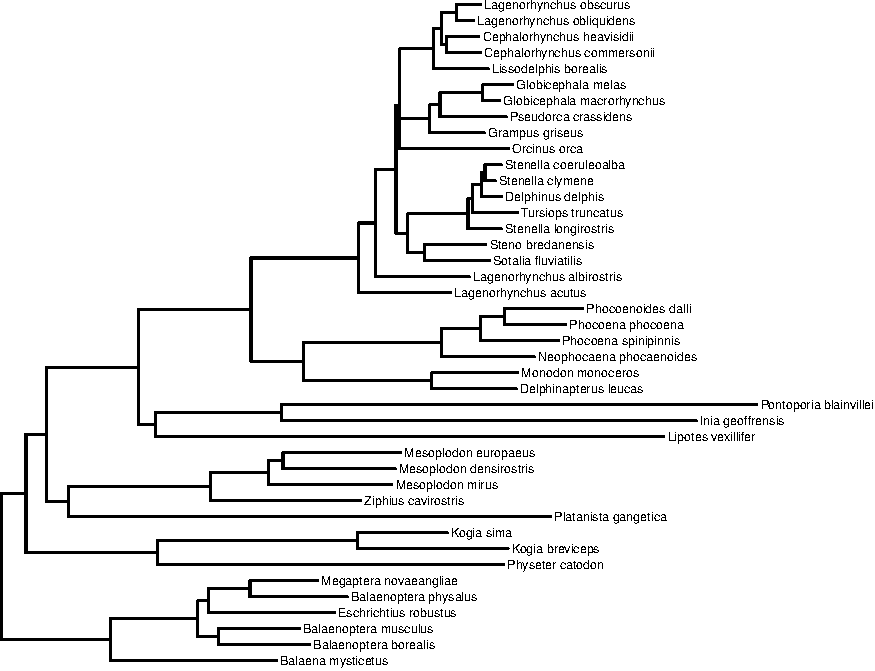
\includegraphics{bookdown-demo_files/figure-latex/unnamed-chunk-127-1} 

}

\caption{Phylogenetic tree of 42 species of cetcaeans with branch lengths proportional to molecular change.}\label{fig:unnamed-chunk-127}
\end{figure}

We're using BayesTraits again so the first step is to get our data into the right format.

\begin{Shaded}
\begin{Highlighting}[]
\NormalTok{BT.data \textless{}{-}}\StringTok{ }\NormalTok{whale.data[,}\KeywordTok{c}\NormalTok{(}\DecValTok{1}\NormalTok{,}\DecValTok{2}\NormalTok{)]}
\KeywordTok{rownames}\NormalTok{(BT.data) \textless{}{-}}\StringTok{ }\OtherTok{NULL}
\end{Highlighting}
\end{Shaded}

As before, we run the random walk (BM) model first. Remember we need to set the working directory to a path where BayesTraits is stored.

\begin{Shaded}
\begin{Highlighting}[]
\KeywordTok{setwd}\NormalTok{(}\StringTok{"\textasciitilde{}/Desktop/BayesTraits"}\NormalTok{)}
\NormalTok{RW.commands \textless{}{-}}\StringTok{ }\KeywordTok{c}\NormalTok{(}\StringTok{"4"}\NormalTok{, }\StringTok{"1"}\NormalTok{)}
\NormalTok{RWmod \textless{}{-}}\StringTok{ }\KeywordTok{bayestraits}\NormalTok{(BT.data, whale.tree, RW.commands)}
\NormalTok{RWmod}\OperatorTok{$}\NormalTok{Log}\OperatorTok{$}\NormalTok{results}
\end{Highlighting}
\end{Shaded}

\begin{verbatim}
  Tree.No       Lh  Alpha.1 Sigma.2.1
1       1 -31.9823 6.422936  6.315406
\end{verbatim}

\begin{Shaded}
\begin{Highlighting}[]
\KeywordTok{setwd}\NormalTok{(wd.reset)}
\end{Highlighting}
\end{Shaded}

The directional model takes a different set of commands.

\begin{Shaded}
\begin{Highlighting}[]
\KeywordTok{setwd}\NormalTok{(}\StringTok{"\textasciitilde{}/Desktop/BayesTraits"}\NormalTok{)}
\NormalTok{D.commands \textless{}{-}}\StringTok{ }\KeywordTok{c}\NormalTok{(}\StringTok{"5"}\NormalTok{, }\StringTok{"1"}\NormalTok{)}
\NormalTok{Dmod \textless{}{-}}\StringTok{ }\KeywordTok{bayestraits}\NormalTok{(BT.data, whale.tree, D.commands)}
\NormalTok{Dmod}\OperatorTok{$}\NormalTok{Log}\OperatorTok{$}\NormalTok{results}
\end{Highlighting}
\end{Shaded}

\begin{verbatim}
  Tree.No        Lh  Alpha.1    Beta.1 Sigma.2.1
1       1 -30.22462 7.951217 -12.37922  5.808331
\end{verbatim}

\begin{Shaded}
\begin{Highlighting}[]
\KeywordTok{setwd}\NormalTok{(wd.reset)}
\end{Highlighting}
\end{Shaded}

Now we need to compare these models! What he have so far is two models and a log likelihood assigned to each. This means we can compare them using a \textbf{likelihood ratio test}. The general formula for an LR test is;

\[\text{LR}=2\times(\text{Lh}_{\text{ Model B}} - \text{Lh}_{\text{ Model A}})\]

The result is the \textbf{likelhood ratio statistic} (LR) which is asymptotically \(\chi^2\) distributed with degrees of freedom equal to the difference in the number of parameters between the models. Model A has 1 parameter (the root value) and model B has 2 (the root and the direction of change) so the degrees of freedom are 1.

\begin{Shaded}
\begin{Highlighting}[]
\DecValTok{2}\OperatorTok{*}\NormalTok{(Dmod}\OperatorTok{$}\NormalTok{Log}\OperatorTok{$}\NormalTok{results}\OperatorTok{$}\NormalTok{Lh[}\DecValTok{1}\NormalTok{] }\OperatorTok{{-}}\StringTok{ }\NormalTok{RWmod}\OperatorTok{$}\NormalTok{Log}\OperatorTok{$}\NormalTok{results}\OperatorTok{$}\NormalTok{Lh[}\DecValTok{1}\NormalTok{])}
\end{Highlighting}
\end{Shaded}

\begin{verbatim}
[1] 3.515352
\end{verbatim}

\begin{Shaded}
\begin{Highlighting}[]
\DecValTok{1}\OperatorTok{{-}}\KeywordTok{pchisq}\NormalTok{(}\FloatTok{3.515352}\NormalTok{, }\DataTypeTok{df =} \DecValTok{1}\NormalTok{) }
\end{Highlighting}
\end{Shaded}

\begin{verbatim}
[1] 0.06080274
\end{verbatim}

Note: pchisq gives the proportion of the distribution to the left of the value. To test if the model is better than the null model, we use 1 - pchisq.

The \textbf{btw} package has a function that will do all this for us. Be careful with interpretation though. Note that the p-value is different. Take this away from 1 and you have your p-value as above.

\begin{Shaded}
\begin{Highlighting}[]
\KeywordTok{lrtest}\NormalTok{(RWmod, Dmod)}
\end{Highlighting}
\end{Shaded}

\begin{verbatim}
  model1.Lh model2.Lh   LRstat      pval
1  -31.9823 -30.22462 3.515352 0.9391973
\end{verbatim}

So what have we got here? Well we have tested two models of the evolution of body size in cetacea. The first is a random walk (Brownian motion) model of evolution in which we have estimated two parameters. The second is a directional model in which we have estimated 3 parameters. Model comparison showed no significant difference between them (LR = 3.52, p = 0.06) and so we should favour the simpler, 2 parameter model. Thus we have no evidence for a directional trend in cetacean body mass evolution.

\hypertarget{changes-in-the-rate-of-evolution-of-a-trait}{%
\section{Changes in the rate of evolution of a trait}\label{changes-in-the-rate-of-evolution-of-a-trait}}

Often when investigating the evolution of a continuous trait, we might have reason to suggest that in some lineages, the rate of evolution of that trait changed.

\begin{center}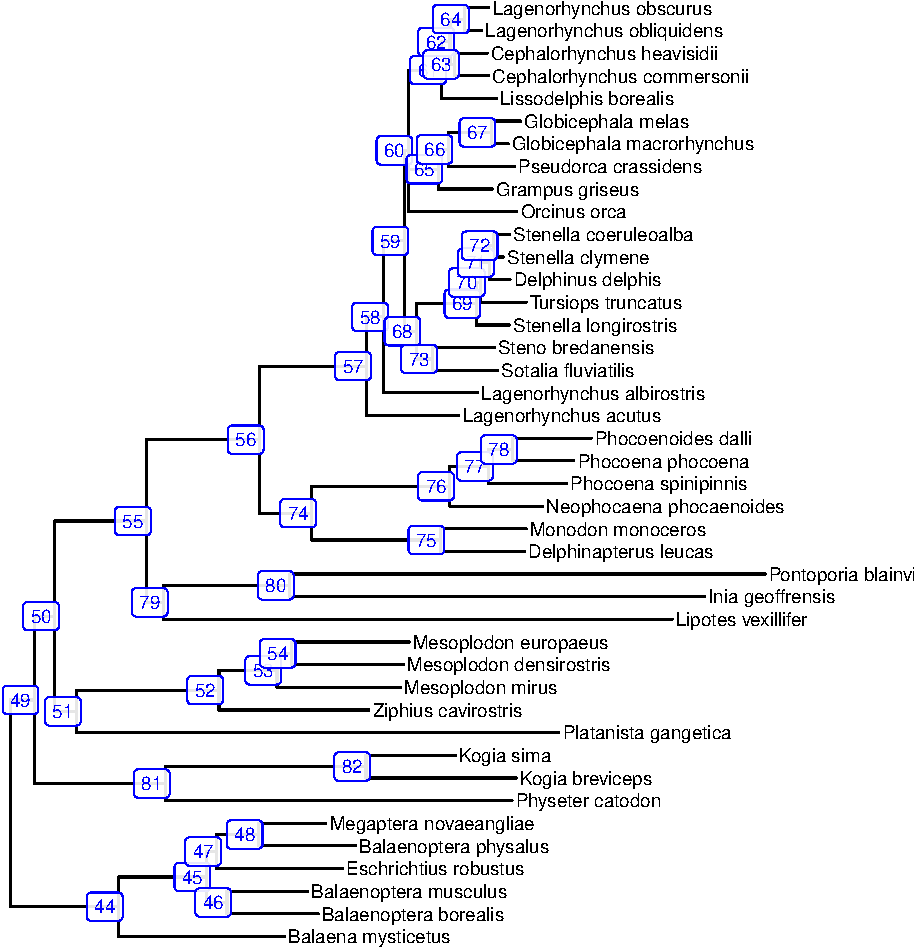
\includegraphics{bookdown-demo_files/figure-latex/unnamed-chunk-133-1} \end{center}

Let's say we have a hypothesis that says the rate of change of body mass changed at the root of mysticetes (node 44). We can paint that onto the tree for demonstration using \textbf{paintSubTree} and \textbf{plotSimmap} in \textbf{phytools} \citep{phytools}.

\begin{Shaded}
\begin{Highlighting}[]
\KeywordTok{require}\NormalTok{(phytools)}
\NormalTok{tree1 \textless{}{-}}\StringTok{ }\KeywordTok{paintSubTree}\NormalTok{(whale.tree, }\DecValTok{44}\NormalTok{, }\StringTok{"2"}\NormalTok{)}
\KeywordTok{plotSimmap}\NormalTok{(tree1, }\DataTypeTok{lwd =} \DecValTok{2}\NormalTok{, }\DataTypeTok{fsize =} \FloatTok{0.7}\NormalTok{)}
\end{Highlighting}
\end{Shaded}

\begin{center}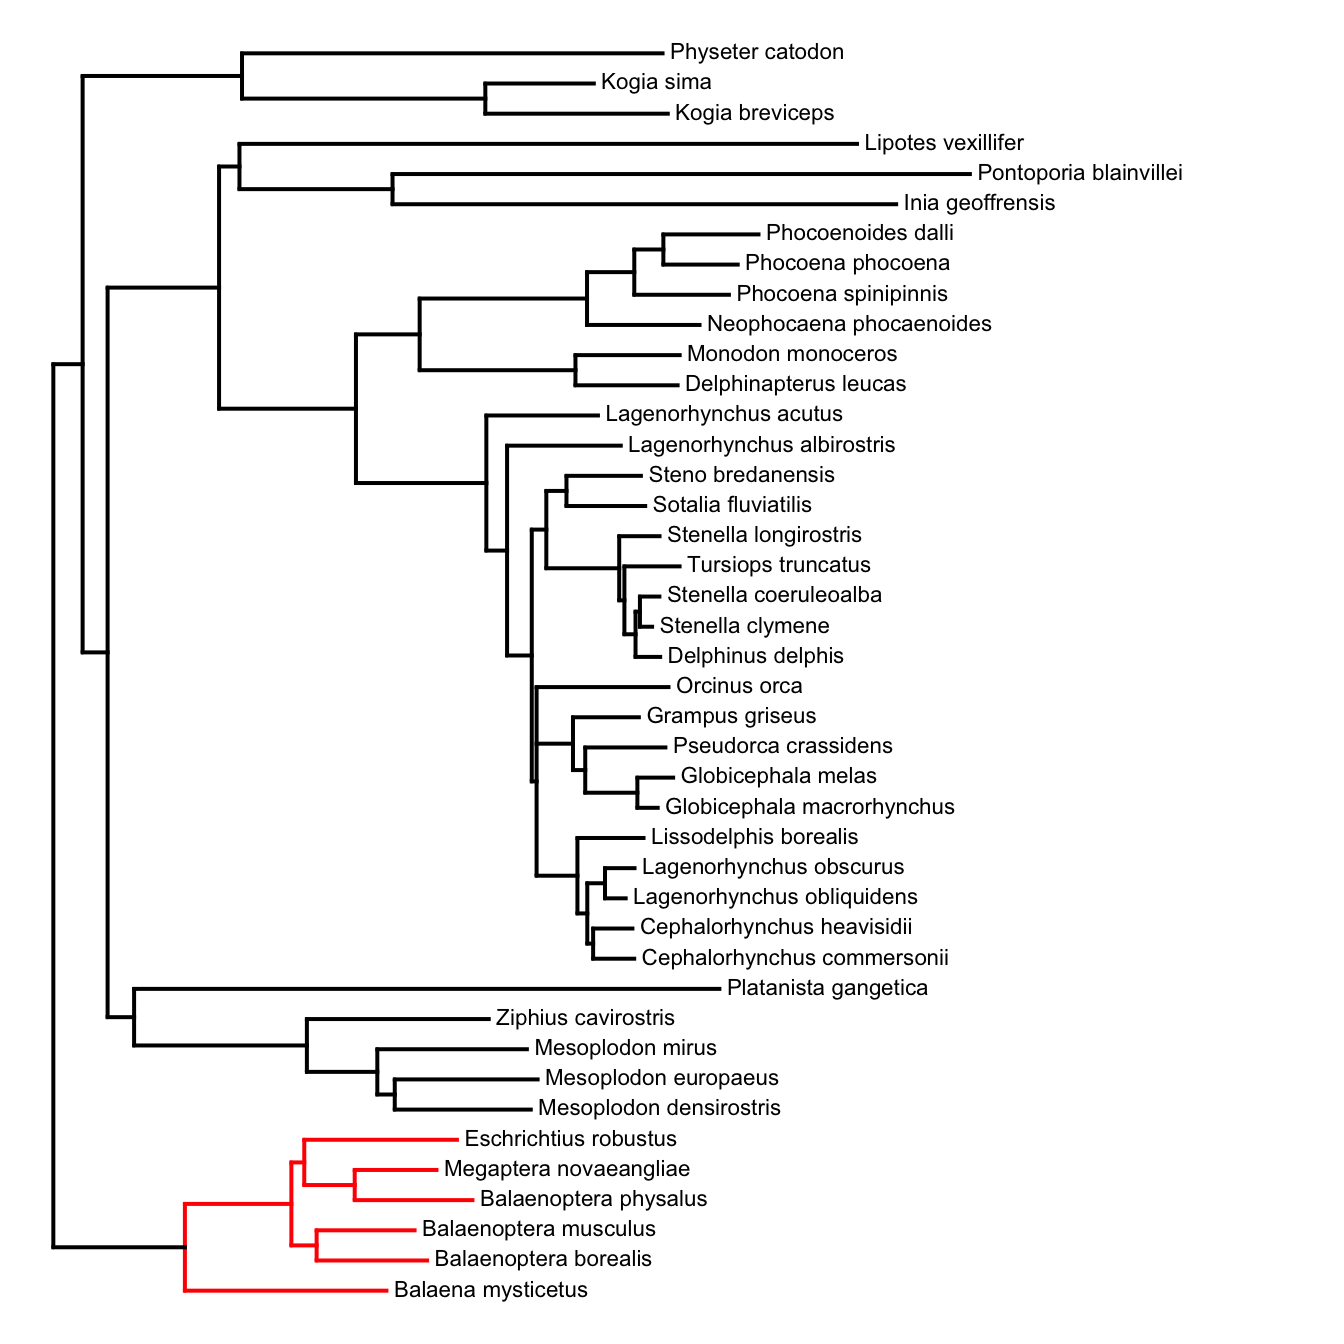
\includegraphics{bookdown-demo_files/figure-latex/unnamed-chunk-134-1} \end{center}

Now we can run the test. Here the function \textbf{brownie.lite} in \textbf{phytools} compares the single rate model to the multi-rate model we have specified!

\begin{Shaded}
\begin{Highlighting}[]
\NormalTok{x \textless{}{-}}\StringTok{ }\NormalTok{whale.data}\OperatorTok{$}\NormalTok{log.body.mass}
\KeywordTok{names}\NormalTok{(x) \textless{}{-}}\StringTok{ }\NormalTok{whale.data}\OperatorTok{$}\NormalTok{species}
\NormalTok{fit \textless{}{-}}\StringTok{ }\KeywordTok{brownie.lite}\NormalTok{(tree1, x)}
\NormalTok{fit}
\end{Highlighting}
\end{Shaded}

\begin{verbatim}
ML single-rate model:
    s^2 se  a   k   logL
value   6.165   1.3453  6.4229  2   -31.9823    

ML multi-rate model:
    s^2(1)  se(1)   s^2(2)  se(2)   a   k   logL    
value   7.1119  1.6786  1.2663  0.8687  6.6116  3   -30.475

P-value (based on X^2): 0.0825 

R thinks it has found the ML solution.
\end{verbatim}

Here we've found no evidence of a regime shift in mysticete cetaceans (p = 0.083).

\hypertarget{uncertainty}{%
\section{Uncertainty}\label{uncertainty}}

If you are familiar with cetaceans and their evolutionary history, you might be surprised by our findings so far in this chapter. The prevailing state of knowledge suggests that cetaceans have evolved large body sizes since the transition to the water of an approximately dog-sized ancestor at the root of our tree. Given what we know about the fossil record of cetacea, we would expect to detect an increase in body size over the tree. To solve this puzzle, we need to look at what information we provided our analysis with.

As the old saying goes, \emph{if you put garbage in, you'll get garbage out} and this seems to apply here. For example, let's look closely at our reconstructions. You can see here that both reconstructions have estimated the mass of the ancestor of cetaceans. Remember that these are log transformed data so we have to transform them back if we want to get a straightforward measurement of mass.

\begin{Shaded}
\begin{Highlighting}[]
\DecValTok{10}\OperatorTok{\^{}}\NormalTok{(RWmod}\OperatorTok{$}\NormalTok{Log}\OperatorTok{$}\NormalTok{results}\OperatorTok{$}\NormalTok{Alpha}\FloatTok{.1}\NormalTok{)}
\end{Highlighting}
\end{Shaded}

\begin{verbatim}
[1] 2648111
\end{verbatim}

\begin{Shaded}
\begin{Highlighting}[]
\DecValTok{10}\OperatorTok{\^{}}\NormalTok{(Dmod}\OperatorTok{$}\NormalTok{Log}\OperatorTok{$}\NormalTok{results}\OperatorTok{$}\NormalTok{Alpha}\FloatTok{.1}\NormalTok{)}
\end{Highlighting}
\end{Shaded}

\begin{verbatim}
[1] 89375216
\end{verbatim}

So depending on our model of evolution the ancestor was either 2,648.1 kg or 89,375.2 kg. A big difference between models so which one we choose really matters.

This is even more of a problem when we look at the fossil record of cetaceans. \emph{Indohyus} (Raoellidae) is thought to be the species that most closely represents the transition to the water by cetacean ancestors \citep{Thewissen09} and its mass is estimated at around 10kg. An early species of cetacean called \emph{Pakicetus} was estimated at around 45kg. So we are orders of magnitude away from what the fossil record shows us!

This problem is well understood in phylogenetic comparative methods. In fact, all methods of ancestral state reconstruction perform very poorly when compared to what we know from the fossil record \citep{Webster02}. As you might expect, the deeper into your tree you try to estimate an ancestral state, the greater the uncertainty. This is especially clear when you look at estimating the root \citep{Gascuel14}. The solution is to incorporate fossil data in the analysis \citep{Slater12}.

\hypertarget{fossils}{%
\subsection{Fossils}\label{fossils}}

To demonstrate the importance of fossil data, let's take a closer look at the evolution of body size in cetaceans. With \textbf{fastAnc}, we found a mass of around 2,650kg for the root of the cetaceans.

The package \textbf{RRphylo} \citep{rrphylo} contains data on fossil and living cetaceans \citep{Serio19}. Using these data, we can hopefully perform a more rigorous ancestral state reconstruction \citep{Castiglione20}. Note that the values here differ between datasets because the previous dataset used a log10 transformation whereas this one uses a natural log transformation!

\begin{Shaded}
\begin{Highlighting}[]
\KeywordTok{library}\NormalTok{(RRphylo)}
\KeywordTok{data}\NormalTok{(}\StringTok{"DataCetaceans"}\NormalTok{)}
\NormalTok{DataCetaceans}\OperatorTok{$}\NormalTok{treecet {-}\textgreater{}}\StringTok{ }\NormalTok{treecet}
\NormalTok{DataCetaceans}\OperatorTok{$}\NormalTok{masscet {-}\textgreater{}}\StringTok{ }\NormalTok{masscet}
\end{Highlighting}
\end{Shaded}

The \textbf{RRphylo} function performs a variant of ancestral state reconstruction called \textbf{phylogenetic ridge regression} \citep{Castiglione20}.

\begin{Shaded}
\begin{Highlighting}[]
\NormalTok{RR \textless{}{-}}\StringTok{ }\KeywordTok{RRphylo}\NormalTok{(treecet, masscet)}
\end{Highlighting}
\end{Shaded}

RRphylo returns a lot of information as a list. Included in this list is the \textbf{tree} used (useful for plotting) and \textbf{aces} which contains the estimates for the traits at the nodes.

\begin{Shaded}
\begin{Highlighting}[]
\KeywordTok{plot}\NormalTok{(RR}\OperatorTok{$}\NormalTok{tree, }\DataTypeTok{cex =} \FloatTok{.4}\NormalTok{, }\DataTypeTok{label.offset =} \FloatTok{.5}\NormalTok{, }\DataTypeTok{no.margin =} \OtherTok{TRUE}\NormalTok{)}
\KeywordTok{nodelabels}\NormalTok{(}\KeywordTok{round}\NormalTok{(RR}\OperatorTok{$}\NormalTok{aces, }\DataTypeTok{digits =} \DecValTok{1}\NormalTok{), }\DataTypeTok{cex =} \FloatTok{.5}\NormalTok{)}
\end{Highlighting}
\end{Shaded}

\begin{center}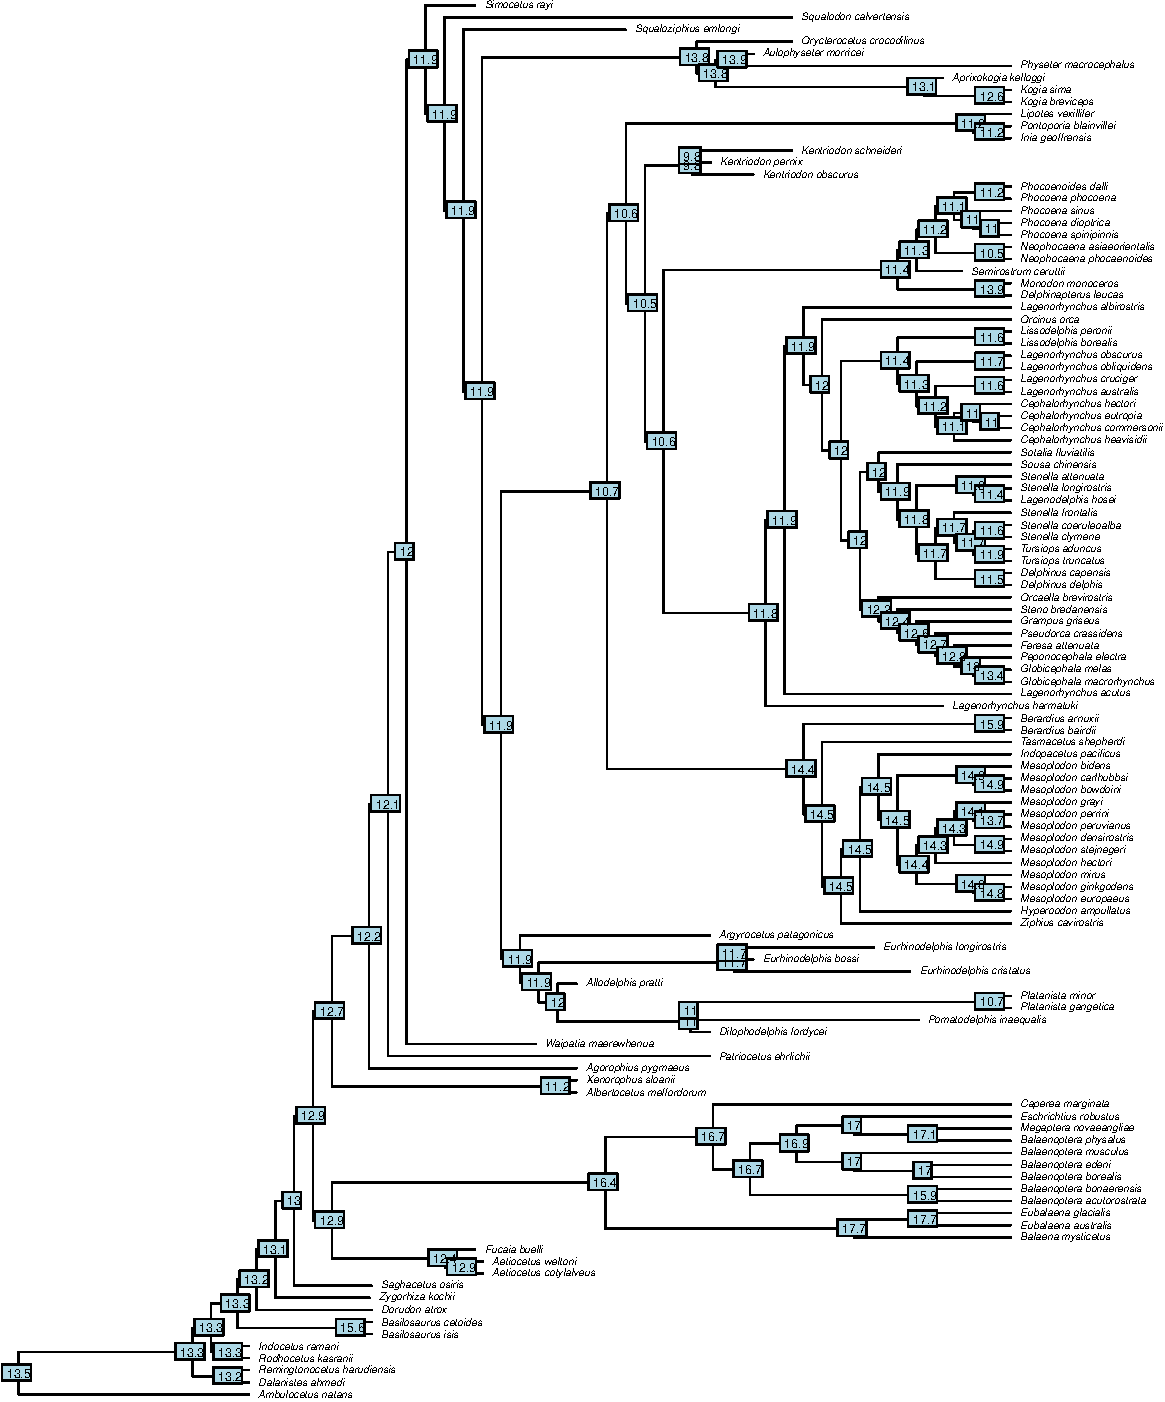
\includegraphics{bookdown-demo_files/figure-latex/unnamed-chunk-139-1} \end{center}

Using this reconstruction, we can extract the mass of the root. Remember that we need \textbf{exp} to calculate the untransformed value rather than raising to the power of 10 because of the natural log transformation.

\begin{Shaded}
\begin{Highlighting}[]
\KeywordTok{exp}\NormalTok{(RR}\OperatorTok{$}\NormalTok{aces[[}\DecValTok{1}\NormalTok{]])}
\end{Highlighting}
\end{Shaded}

\begin{verbatim}
[1] 727063.9
\end{verbatim}

So our new estimate of the mass of the ancestor of cetaceans is 727.1kg. This is much closer to the estimated mass of early archeocete cetaceans like \emph{Ambulocetus natans} at about 430kg and \emph{Indocetus ramani} at around 630kg.

If we still aren't satisfied that we have included the best information we have available, we can actually \emph{fossilise} a node by passing a named list of ancestral states to the \textbf{RRphylo} function. Following the example of Castiglione \emph{et al}. \citeyearpar{Castiglione20}, we can set the node of the ancestor of mysticetes to a known mass. Here we are assuming that the most recent common ancestor of all mysticetes can be represented by the species \emph{Mystacodon selenensis} which weighed arond 150kg. Also we need to know that this ancestor is represented by the node labelled 128 in our tree object.

\begin{Shaded}
\begin{Highlighting}[]
\NormalTok{x \textless{}{-}}\StringTok{ }\KeywordTok{log}\NormalTok{(}\DecValTok{150000}\NormalTok{)}
\KeywordTok{names}\NormalTok{(x) \textless{}{-}}\StringTok{ "128"}
\end{Highlighting}
\end{Shaded}

Now we can pass this state to the argument \textbf{aces} in \textbf{RRphylo} and the analysis will hold node 128 at the value we have set. You should be able to see that in the following plot, the ancestor of mysticetes is reconstructed as 11.9 rather than 12.9 in the previous reconstruction.

\begin{Shaded}
\begin{Highlighting}[]
\NormalTok{RR2 \textless{}{-}}\StringTok{ }\KeywordTok{RRphylo}\NormalTok{(treecet, masscet, }\DataTypeTok{aces =}\NormalTok{ x)}
\KeywordTok{plot}\NormalTok{(RR2}\OperatorTok{$}\NormalTok{tree, }\DataTypeTok{cex =} \FloatTok{.4}\NormalTok{, }\DataTypeTok{label.offset =} \FloatTok{.5}\NormalTok{, }\DataTypeTok{no.margin =} \OtherTok{TRUE}\NormalTok{)}
\KeywordTok{nodelabels}\NormalTok{(}\KeywordTok{round}\NormalTok{(RR2}\OperatorTok{$}\NormalTok{aces, }\DataTypeTok{digits =} \DecValTok{1}\NormalTok{), }\DataTypeTok{cex =} \FloatTok{.5}\NormalTok{)}
\end{Highlighting}
\end{Shaded}

\begin{center}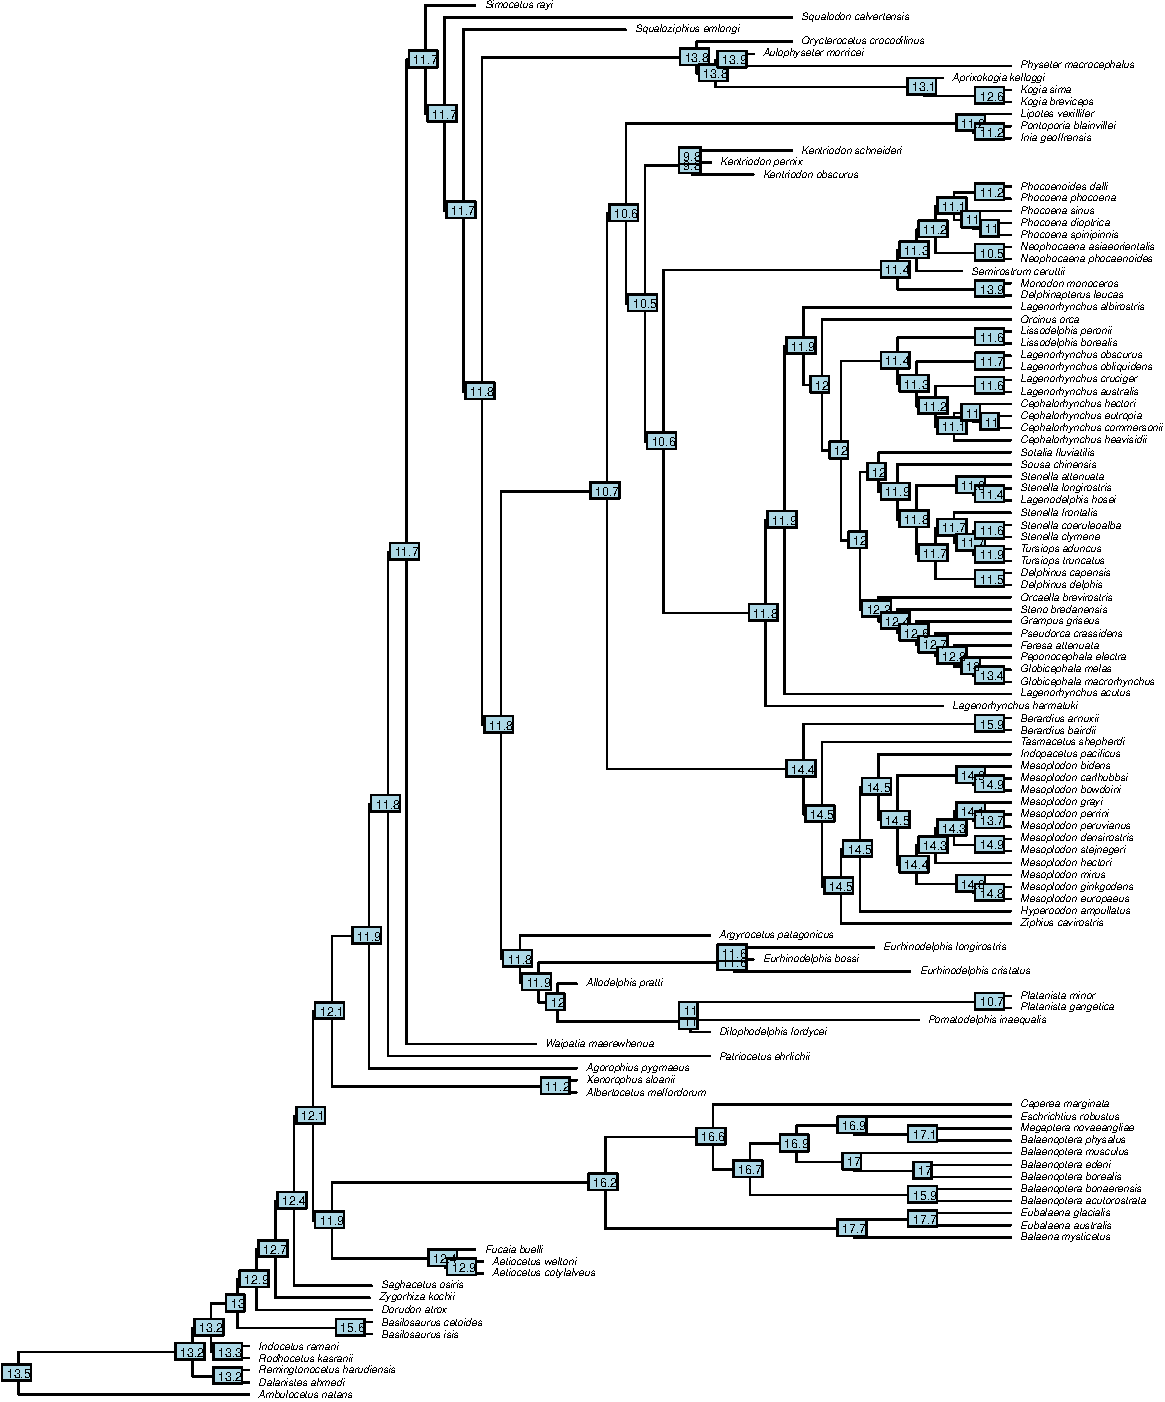
\includegraphics{bookdown-demo_files/figure-latex/unnamed-chunk-142-1} \end{center}

Hopefully you can see that the more fossil information you include in your reconstructions, the more reliable they are.

\hypertarget{revisiting-mysticete-body-mass}{%
\subsection{Revisiting Mysticete Body Mass}\label{revisiting-mysticete-body-mass}}

In using the fossil data we have added in here, Castiglione \emph{et al}. \citeyearpar{Castiglione20} demonstrated that mysticetes actually do conform to Cope's rule because they have an increasing trend in body size over time. This shows just how important adding in fossil data can be if you want the full picture.

This seems to suggest that we should also find a regime shift in mysticetes. Let's have a closer look. We begin again by painting the tree at the specific node leading to mysticetes.

\begin{Shaded}
\begin{Highlighting}[]
\KeywordTok{require}\NormalTok{(phytools)}
\NormalTok{tree2 \textless{}{-}}\StringTok{ }\KeywordTok{paintSubTree}\NormalTok{(treecet, }\DecValTok{128}\NormalTok{, }\StringTok{"2"}\NormalTok{)}
\KeywordTok{plotSimmap}\NormalTok{(tree2, }\DataTypeTok{lwd =} \DecValTok{2}\NormalTok{, }\DataTypeTok{fsize =} \FloatTok{0.5}\NormalTok{)}
\end{Highlighting}
\end{Shaded}

\begin{center}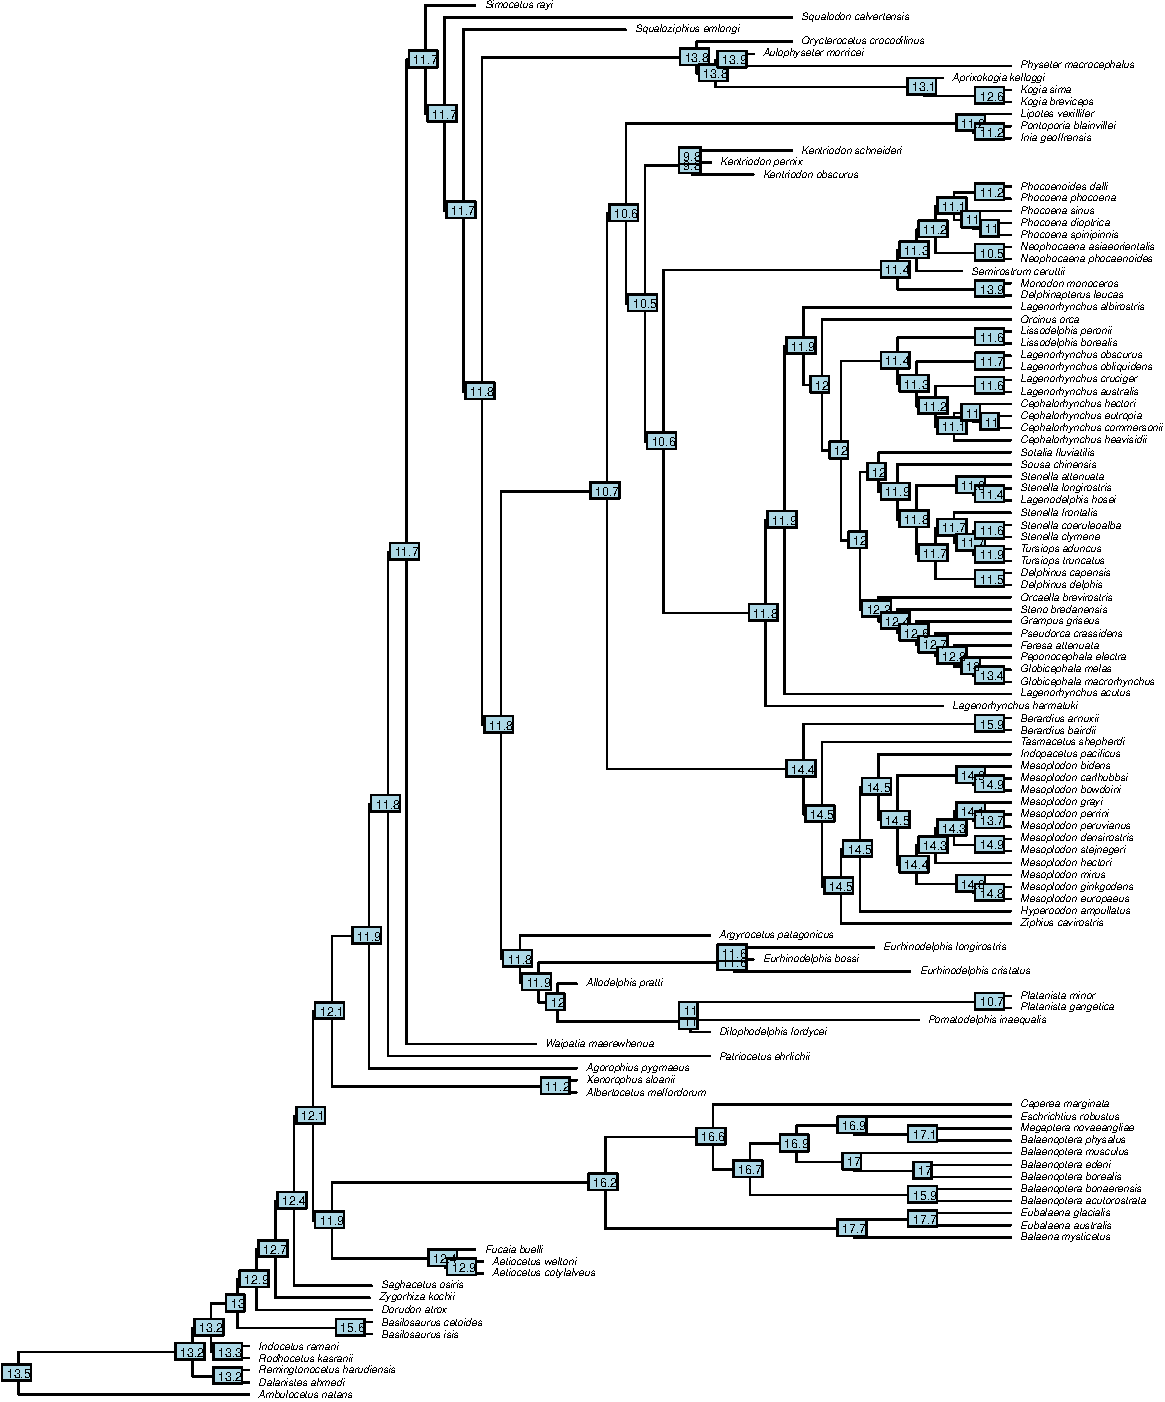
\includegraphics{bookdown-demo_files/figure-latex/unnamed-chunk-143-1} \end{center}

Next we run \textbf{brownie.lite} on our expanded dataset.

\begin{Shaded}
\begin{Highlighting}[]
\NormalTok{fit \textless{}{-}}\StringTok{ }\KeywordTok{brownie.lite}\NormalTok{(tree2, masscet)}
\NormalTok{fit}
\end{Highlighting}
\end{Shaded}

\begin{verbatim}
ML single-rate model:
    s^2 se  a   k   logL
value   0.2047  0.0265  13.2057 2   -178.7922   

ML multi-rate model:
    s^2(1)  se(1)   s^2(2)  se(2)   a   k   logL    
value   0.176   0.0245  0.4012  0.147   13.2056 3   -176.0958

P-value (based on X^2): 0.0202 

R thinks it has found the ML solution.
\end{verbatim}

There you have it! We can now say that we have evidence in favour of a regime shift in mysticete body size (p = 0.02).

\hypertarget{further-info-4}{%
\section{Further info}\label{further-info-4}}

We've only just scratched the surface of what is possible with ancestral state reconstruction. For some background reading, have a look at chapter 4 of \emph{The comparative approach in evolutionary anthropology and biology} \citep{Nunn11}.

\hypertarget{diversification}{%
\chapter{Diversification}\label{diversification}}

\hypertarget{introduction}{%
\section{Introduction}\label{introduction}}

Phylogenetic comparative methods can be used to study the diversification of lineages over time. This can be particularly useful when studying adaptive radiations which are thought to change the rate of speciation. This chapter will begin by studying some diversification models.

\hypertarget{pure-birth-model}{%
\subsection{Pure Birth Model}\label{pure-birth-model}}

The simplest form of diversification model is a \textbf{pure birth} model. Under this model, each lineage has a constant probability of speciating. This probability gives us the \textbf{birth rate} (\emph{b}). Over time (\emph{t}), lineages will speciate and thus the number of lineages (\emph{N}) will increase exponentially.

\[ N_{(\text{t})} = N_{(0)}e^{\text{bt}} \]
This plot shows how the number of species would grow over time. Note that in this model, there is no extinction and so the exponential increase is because each speciation event produces two daughter lineages which each can then speciate with probabilty \emph{b}, creating two more daughter lineages each and so on.

\begin{center}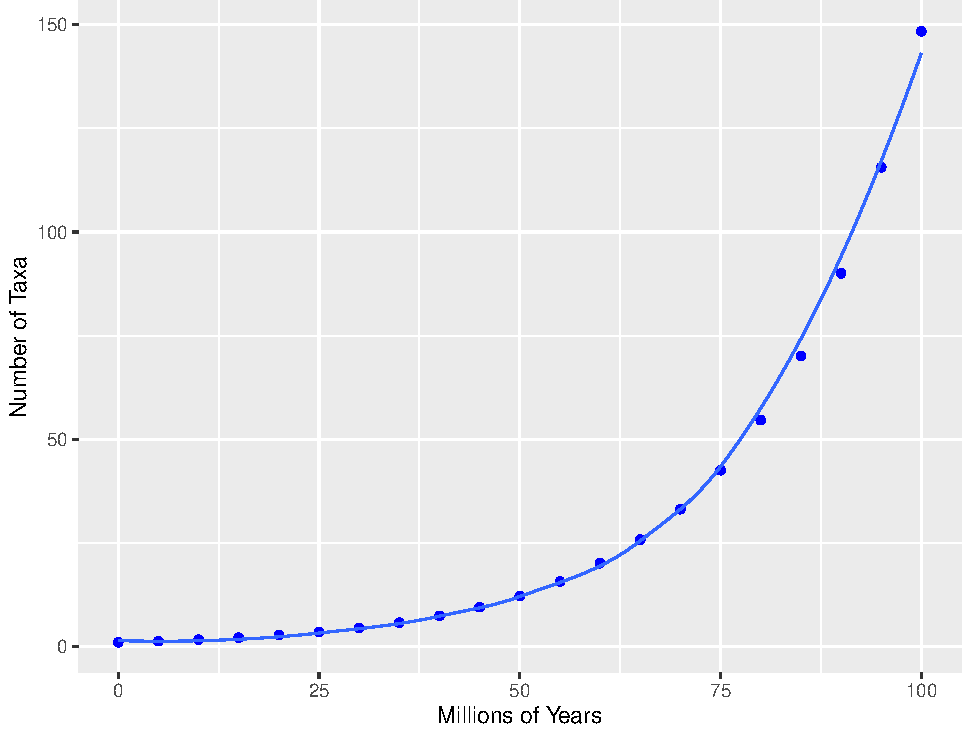
\includegraphics{bookdown-demo_files/figure-latex/unnamed-chunk-146-1} \end{center}

As you can probably tell, the pure birth model is not a very good representation of biological reality. For example, today there are around 90 species of cetacean. A pure birth model in which we have \emph{b} set at 0.1 (meaning we have 0.1 new species born every million years) would give us over 1 million species of cetacean in 100 million years.

\hypertarget{the-birth-death-model}{%
\subsection{The Birth-Death Model}\label{the-birth-death-model}}

The \textbf{birth-death} model incorporates extinction as well as speciation. Under the simplest form of this model, speciation and extinction occur randomly. Each lineage is assumed to have a constant rate of speciation (\emph{b}) and extinction (\emph{d}). Under this model, the number of lineages will increase exponentially with the difference between birth and death rate (\emph{b - d}).

\[ N_{(\text{t})} = N_{(0)}e^{\text{(b-d)t}} \]
This graph shows the change in number of taxa over time when the birth rate slightly exceeds death rate.

\begin{center}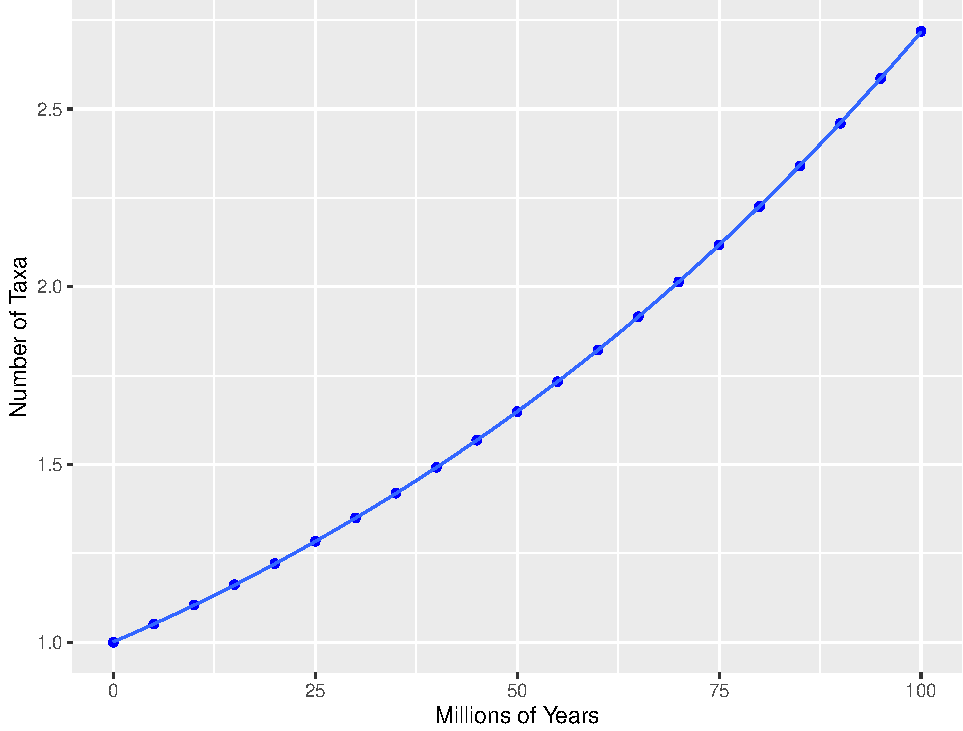
\includegraphics{bookdown-demo_files/figure-latex/unnamed-chunk-147-1} \end{center}

\hypertarget{the-signature-of-extinction}{%
\subsection{The signature of extinction}\label{the-signature-of-extinction}}

Let's investigate the differences between pure birth and birth-death models by simulating some trees.

The function \textbf{sim.bd.age} in the package \textbf{TreeSim} \citep{treesim} allows us to simulate birth-death trees with a fixed age. First we will set the birth rate \(\lambda\) to 0.4 and the death rate \(\mu\) to 0 as this is a pure-birth tree. Note that these were \emph{b} and \emph{d} in the previous sections but \(\lambda\) and \(\mu\) are widely used.

\begin{Shaded}
\begin{Highlighting}[]
\KeywordTok{library}\NormalTok{(ape)}
\KeywordTok{library}\NormalTok{(TreeSim)}
\NormalTok{tree1 \textless{}{-}}\StringTok{ }\KeywordTok{sim.bd.age}\NormalTok{(}\DataTypeTok{age =} \DecValTok{10}\NormalTok{, }\DataTypeTok{numbsim =} \DecValTok{1}\NormalTok{, }\DataTypeTok{lambda =} \FloatTok{0.4}\NormalTok{, }\DataTypeTok{mu =} \DecValTok{0}\NormalTok{)[[}\DecValTok{1}\NormalTok{]]}
\NormalTok{ggtree}\OperatorTok{::}\KeywordTok{ggtree}\NormalTok{(tree1)}
\end{Highlighting}
\end{Shaded}

\begin{center}\includegraphics{bookdown-demo_files/figure-latex/unnamed-chunk-149-1} \end{center}

If you run this command yourself, your tree will look different simply because the simulations will differ each time.

We can plot the pattern of lineage accumulation through time with a lineage-through-time plot. This can be plotted using the function \textbf{ltt.plot} in ape \citep{ape}. Note that because of the expectation of exponential growth, we should log scale the y-axis

\begin{Shaded}
\begin{Highlighting}[]
\KeywordTok{ltt.plot}\NormalTok{(tree1, }\DataTypeTok{log =} \StringTok{"y"}\NormalTok{)}
\end{Highlighting}
\end{Shaded}

\begin{center}\includegraphics{bookdown-demo_files/figure-latex/unnamed-chunk-150-1} \end{center}

As can be seen from this plot, the increase in lineages over time will be log-linear, just as predicted in previous sections.

What about when we add extinction? We can see here that pure-birth and birth-death trees look quite different. this is because older lineages are more likely to go extinct. This \emph{pull of the present} means that extinction rates appear lower in the present even though there's no reason to assume that they would be any different. We just have a greater proportion of total lineages the closer we are to the present!

\begin{center}\includegraphics{bookdown-demo_files/figure-latex/unnamed-chunk-151-1} \end{center}

\hypertarget{estimating-speciation-and-extinction-rate}{%
\section{Estimating speciation and extinction rate}\label{estimating-speciation-and-extinction-rate}}

Given a phylogeny, we can estimate speciation and extinction rate using the function \textbf{birthdeath} in \textbf{ape} \citep{ape}.

\begin{Shaded}
\begin{Highlighting}[]
\KeywordTok{library}\NormalTok{(ape)}
\NormalTok{whales \textless{}{-}}\StringTok{ }\KeywordTok{read.tree}\NormalTok{(}\StringTok{"whaletree.tre"}\NormalTok{)}
\NormalTok{bd.mod \textless{}{-}}\StringTok{ }\KeywordTok{birthdeath}\NormalTok{(whales)}
\NormalTok{bd.mod}
\end{Highlighting}
\end{Shaded}

\begin{verbatim}
Estimation of Speciation and Extinction Rates
            with Birth-Death Models

     Phylogenetic tree: whales 
        Number of tips: 87 
              Deviance: -45.0534 
        Log-likelihood: 22.5267 
   Parameter estimates:
      d / b = 0   StdErr = 0 
      b - d = 0.103623   StdErr = 0.007955189 
   (b: speciation rate, d: extinction rate)
   Profile likelihood 95% confidence intervals:
      d / b: [-0.4859418, 0.2661802]
      b - d: [0.08313059, 0.1272357]
\end{verbatim}

The output here gives us some derived values such as \(b - d\) (net diversification). If you want to cut straight to the speciation and extinction rates, you can use a \textbf{phytools} function called \textbf{bd} \citep{phytools}.

\begin{Shaded}
\begin{Highlighting}[]
\NormalTok{phytools}\OperatorTok{::}\KeywordTok{bd}\NormalTok{(bd.mod)}
\end{Highlighting}
\end{Shaded}

\begin{verbatim}
       b        d 
0.103623 0.000000 
\end{verbatim}

This is a nice start but it assumes constant rates across the tree and that doesn't seem like a reasonable assumption to me. We also may have good reason to doubt that the extinction rate is truly 0!

\hypertarget{medusa}{%
\section{MEDUSA}\label{medusa}}

The general birth-death models you have seen so far produce a fairly uniform tree of life. In reality, this isn't actually what we observe. Some clades are highly diverse (such as arthropods) and some are not. This implies that the rates of diversification can vary between lineages.

In fact, based on our understanding of evolution, we would expect rates to change all the time! We know that extinction rates fluctuate around a background rate. For example, extinction rates increase dramatically during mass extinctions. Speciation rates increase during adaptive radiations. The next methods to look at are capable of detecting these changes in rate using phylogenies.

\textbf{MEDUSA} stands for Modelling Evolutionary Diversification Using Stepwise AIC \citep{Alfaro09}. It fits piecewise models of birth and death to our tree and allows us to ask where rates of birth and death may have changed and why clades might differ in size.

MEDUSA fits models to the tree, splitting the tree and allowing the rate to change at each split. The method proceeds by comparing the old model to the new model using AICc to either accept of reject the shift in rate.

Let's see how it works using the phylogeny of cetaceans.

We can run the analysis using the \textbf{medusa} function in geiger \citep{geiger}. All we have to specify here is the tree \textbf{phy = whales} and that we want to fit birth-death models \textbf{model = ``bd''}.

\begin{Shaded}
\begin{Highlighting}[]
\KeywordTok{library}\NormalTok{(geiger)}
\NormalTok{m1 \textless{}{-}}\StringTok{ }\KeywordTok{medusa}\NormalTok{(}\DataTypeTok{phy =}\NormalTok{ whales, }\DataTypeTok{model =} \StringTok{"bd"}\NormalTok{)}
\end{Highlighting}
\end{Shaded}

\begin{verbatim}
Appropriate  aicc-threshold for a tree of 87 tips is: 4.397737.

Step 1: lnLik=-277.6943; aicc=559.4591; model=bd
Step 2: lnLik=-266.7389; aicc=543.8371; shift at node 141; model=bd; cut=stem; # shifts=1

No significant increase in aicc score. Disregarding subsequent piecewise models.

Calculating profile likelihoods on parameter values.

  Model.ID Shift.Node Cut.At Model Ln.Lik.part        r     epsilon     r.low
1        1         88   node    bd   -185.5379 0.076678 1.50783e-08 0.0576867
2        2        141   stem    bd   -81.20097 0.232141 4.73531e-06 0.1616522
     r.high eps.low  eps.high
1 0.0994803       0 0.2537393
2 0.3204785       0 0.2713275
\end{verbatim}

There's a lot of information in this output so let's go through it. Firstly, we are told that the appropriate AICc threshold for a tree of this size is 4.4. You may be used to using a change of 2 in AIC as signifiying a significant difference between models. The appropriate threshold for distinguishing between models using MEDUSA varies depending on the size of the tree. Fortunately, the function simply calculates it and reports it to us.

Next we have the stepwise output. In this case we only have 2 steps. Each step is reported to us and in this case, we can see that step 2 involves cutting the tree at node 141. This means that \emph{medusa} has identfied a change in rate at node 141 and continued with the new model from that node.

Finally, the table gives us parameter values for each step. This is very important in interpreting the output. Note that \emph{epsilon} is the extinction rate, previously known as either \emph{d} or \(\mu\) and \emph{r} is the net diversification rate (\(\lambda - \mu\)).

The best way to visualise this analysis is by plotting the models on the tree. When we do so we can see that \emph{medusa} has placed the shift near the root of the Delphinidae (excluding interestingly the orca). We can see that the rate of diversification is much greater in the oceanic dolphins.

\begin{Shaded}
\begin{Highlighting}[]
\KeywordTok{par}\NormalTok{(}\DataTypeTok{mar =} \KeywordTok{c}\NormalTok{(}\FloatTok{3.1}\NormalTok{, }\DecValTok{0}\NormalTok{, }\FloatTok{0.1}\NormalTok{, }\DecValTok{0}\NormalTok{))}
\KeywordTok{plot}\NormalTok{(m1, }\DataTypeTok{label.offset =} \FloatTok{0.1}\NormalTok{)}
\KeywordTok{legend}\NormalTok{(}\DataTypeTok{x =} \FloatTok{{-}0.5}\NormalTok{, }\DataTypeTok{y =} \DecValTok{60}\NormalTok{, }\DataTypeTok{legend=}\StringTok{"r = 0.08"}\NormalTok{,}
       \DataTypeTok{text.col=}\StringTok{"Black"}\NormalTok{, }\DataTypeTok{title =} \StringTok{"Step 1"}\NormalTok{)}
\KeywordTok{legend}\NormalTok{(}\DataTypeTok{x =} \DecValTok{15}\NormalTok{, }\DataTypeTok{y =} \DecValTok{75}\NormalTok{, }\DataTypeTok{legend=}\StringTok{"r = 0.23"}\NormalTok{,}
       \DataTypeTok{text.col=}\StringTok{"red"}\NormalTok{, }\DataTypeTok{title =} \StringTok{"Step 2"}\NormalTok{, }\DataTypeTok{box.col =} \StringTok{"red"}\NormalTok{)}
\end{Highlighting}
\end{Shaded}

\begin{center}\includegraphics[width=1\linewidth]{bookdown-demo_files/figure-latex/unnamed-chunk-158-1} \end{center}

\hypertarget{rpanda}{%
\section{RPANDA}\label{rpanda}}

The package \textbf{RPANDA} \citep{rpanda} allows us to fit different defined models of variation in the rate of birth and death through time. We can then select the best model by maximum likelihood. This is a good way of testing an \emph{a priori} hypothesis we may have about diversification in a lineage.

The first step is to define a few functions that describe our hypotheses. First we need to define speciation rate (\(\lambda\)) as either constant (\textbf{lambda.cst}) or varying exponentially (\textbf{lambda.var}). We can do the same for extinction rate (\(\mu\)).

\[ \lambda_{(\text{t})} = \lambda_{(0)}e^{\alpha \text{t}} \;\;\;\;\;\;\;\;\;\;\;\;\;\;\;\;\;  \mu_{(\text{t})} = \mu_{(0)}e^{\beta \text{t}} \]

\begin{Shaded}
\begin{Highlighting}[]
\NormalTok{lambda.cst \textless{}{-}}\StringTok{ }\ControlFlowTok{function}\NormalTok{(x,y)\{y\}}
\NormalTok{lambda.var \textless{}{-}}\StringTok{ }\ControlFlowTok{function}\NormalTok{(x,y)\{y[}\DecValTok{1}\NormalTok{]}\OperatorTok{*}\KeywordTok{exp}\NormalTok{(y[}\DecValTok{2}\NormalTok{]}\OperatorTok{*}\NormalTok{x)\}}
\NormalTok{mu.cst \textless{}{-}}\StringTok{ }\ControlFlowTok{function}\NormalTok{(x,y)\{y\}}
\NormalTok{mu.var \textless{}{-}}\StringTok{ }\ControlFlowTok{function}\NormalTok{(x,y)\{y[}\DecValTok{1}\NormalTok{]}\OperatorTok{*}\KeywordTok{exp}\NormalTok{(y[}\DecValTok{2}\NormalTok{]}\OperatorTok{*}\NormalTok{x)\}}
\end{Highlighting}
\end{Shaded}

We will test 4 different combinations of these scenarios. I find it easier to visualise models like this graphically so these plots describe the various models.

\begin{center}\includegraphics{bookdown-demo_files/figure-latex/unnamed-chunk-161-1} \end{center}

In RPANDA, we need to specify which clades are most likely to have diversification shifts to test our hypotheses. For this example, we will look at 4 major radiations of cetaceans. These are; \emph{Balaenopteridae, Ziphidae, Phocoenidae} and \emph{Delphinidae}.

\begin{center}\includegraphics{bookdown-demo_files/figure-latex/unnamed-chunk-162-1} \end{center}

\begin{Shaded}
\begin{Highlighting}[]
\KeywordTok{library}\NormalTok{(RPANDA)}
\end{Highlighting}
\end{Shaded}

We can extract the relevant sub-trees using \textbf{extract.clade} in \textbf{ape} \citep{ape} in combination with \textbf{MRCA} in \textbf{phylobase} \citep{phylobase}. Don't forget to also make another subtree of all the species not in those groups.

\begin{Shaded}
\begin{Highlighting}[]
\NormalTok{delphinidae.tree \textless{}{-}}\StringTok{ }\KeywordTok{extract.clade}\NormalTok{(whales, }\DataTypeTok{node =}\NormalTok{ phylobase}\OperatorTok{::}\KeywordTok{MRCA}\NormalTok{(whales, }\DataTypeTok{tip =} \KeywordTok{c}\NormalTok{(}\StringTok{"Orcinus\_orca"}\NormalTok{, }\StringTok{"Delphinus\_delphis"}\NormalTok{)))}
\NormalTok{phocoenidae.tree \textless{}{-}}\StringTok{ }\KeywordTok{extract.clade}\NormalTok{(whales, }\DataTypeTok{node =}\NormalTok{ phylobase}\OperatorTok{::}\KeywordTok{MRCA}\NormalTok{(whales, }\DataTypeTok{tip =} \KeywordTok{c}\NormalTok{(}\StringTok{"Phocoena\_dioptrica"}\NormalTok{, }\StringTok{"Phocoena\_phocoena"}\NormalTok{)))}
\NormalTok{ziphidae.tree \textless{}{-}}\StringTok{ }\KeywordTok{extract.clade}\NormalTok{(whales, }\DataTypeTok{node =}\NormalTok{ phylobase}\OperatorTok{::}\KeywordTok{MRCA}\NormalTok{(whales, }\DataTypeTok{tip =} \KeywordTok{c}\NormalTok{(}\StringTok{"Mesoplodon\_grayi"}\NormalTok{, }\StringTok{"Tasmacetus\_shepherdi"}\NormalTok{)))}
\NormalTok{balaenopteridae.tree \textless{}{-}}\StringTok{ }\KeywordTok{extract.clade}\NormalTok{(whales, }\DataTypeTok{node =}\NormalTok{ phylobase}\OperatorTok{::}\KeywordTok{MRCA}\NormalTok{(whales, }\DataTypeTok{tip =} \KeywordTok{c}\NormalTok{(}\StringTok{"Balaenoptera\_physalus"}\NormalTok{, }\StringTok{"Balaenoptera\_edeni"}\NormalTok{)))}

\NormalTok{othercetaceans.tree \textless{}{-}}\StringTok{ }\KeywordTok{drop.tip}\NormalTok{(whales,}\KeywordTok{c}\NormalTok{(balaenopteridae.tree}\OperatorTok{$}\NormalTok{tip.label,}
\NormalTok{                                         delphinidae.tree}\OperatorTok{$}\NormalTok{tip.label, }
\NormalTok{                                         phocoenidae.tree}\OperatorTok{$}\NormalTok{tip.label, }
\NormalTok{                                         ziphidae.tree}\OperatorTok{$}\NormalTok{tip.label))}
\end{Highlighting}
\end{Shaded}

Now we can fit some birth-death models! Let's start with both parameters constant (\textbf{bcstdcst}). The function we need is \textbf{fit\_bd}. This function requires a lot of information so let's take it slowly.

The first argument is just our tree (\textbf{phylo}). Then we need to include the total length of the tree (\textbf{tot\_time}). We don't know this offhand but we can calculate it using \textbf{max(branching.times(TREE))}. The arguments \textbf{f.lamb} and \textbf{f.mu} take our previously defined functions for \(\lambda\) (birth rate) and \(\mu\) (death rate). \textbf{lamb\_par} and \textbf{mu\_par} similarly take our initial values for \(\lambda\) and \(\mu\) which here, will be 0.4 and 0 respectively. \textbf{cst.lamb} and \textbf{cst.mu} are both logical (they can be true or false) and ask if \(\lambda\) and \(\mu\) are constant (they are). The argument \textbf{f} is the fraction of extant species included in the whole phylogeny. Here we have 87 out of the 89 cetacean species. Finally, \textbf{dt} is set to the recommended value in the vignette for the function. In short, \textbf{dt} is the length of the time interval on which functions are assumed to be constant. Smaller values mean a finer-grain analysis and longer computing times. Larger values mean the analysis will be quicker but lower resolution.

\begin{Shaded}
\begin{Highlighting}[]
\NormalTok{bcstdcst \textless{}{-}}\StringTok{ }\KeywordTok{fit\_bd}\NormalTok{(}\DataTypeTok{phylo =}\NormalTok{ delphinidae.tree, }
                   \DataTypeTok{tot\_time =} \KeywordTok{max}\NormalTok{(}\KeywordTok{branching.times}\NormalTok{(delphinidae.tree)),}
                   \DataTypeTok{f.lamb =}\NormalTok{ lambda.cst, }\DataTypeTok{f.mu =}\NormalTok{ mu.cst,}
                   \DataTypeTok{lamb\_par =} \FloatTok{0.4}\NormalTok{, }\DataTypeTok{mu\_par =} \DecValTok{0}\NormalTok{,}
                   \DataTypeTok{cst.lamb =} \OtherTok{TRUE}\NormalTok{, }\DataTypeTok{cst.mu =} \OtherTok{TRUE}\NormalTok{,}
                   \DataTypeTok{f =} \DecValTok{87}\OperatorTok{/}\DecValTok{89}\NormalTok{, }\DataTypeTok{dt =} \FloatTok{1e{-}3}\NormalTok{)}
\end{Highlighting}
\end{Shaded}

The analysis has returned a number of details. Most importantly for us, the likelihood and AICc will allow for model comparison.

\begin{Shaded}
\begin{Highlighting}[]
\NormalTok{bcstdcst}
\end{Highlighting}
\end{Shaded}

\begin{verbatim}
model :
[1] "birth death"

LH :
[1] -83.51998

aicc :
[1] 171.415

lamb_par :
[1] 0.2189443

mu_par :
[1] 2.413309e-09
\end{verbatim}

Let's now evaluate the other 3 models using the same function. Be mindful of the changes in argument for each model. Especially the \textbf{expo.} and \textbf{cst.} arguments which differ depending on the model.

\begin{Shaded}
\begin{Highlighting}[]
\NormalTok{bvardcst \textless{}{-}}\StringTok{ }\KeywordTok{fit\_bd}\NormalTok{(}\DataTypeTok{phylo =}\NormalTok{ delphinidae.tree, }
                   \DataTypeTok{tot\_time =} \KeywordTok{max}\NormalTok{(}\KeywordTok{branching.times}\NormalTok{(delphinidae.tree)),}
                   \DataTypeTok{f.lamb =}\NormalTok{ lambda.var, }\DataTypeTok{f.mu =}\NormalTok{ mu.cst,}
                   \DataTypeTok{lamb\_par =} \KeywordTok{c}\NormalTok{(}\FloatTok{0.4}\NormalTok{,}\OperatorTok{{-}}\FloatTok{0.05}\NormalTok{), }\DataTypeTok{mu\_par =} \DecValTok{0}\NormalTok{,}
                   \DataTypeTok{expo.lamb =} \OtherTok{TRUE}\NormalTok{, }\DataTypeTok{cst.mu =} \OtherTok{TRUE}\NormalTok{,}
                   \DataTypeTok{f =} \DecValTok{87}\OperatorTok{/}\DecValTok{89}\NormalTok{, }\DataTypeTok{dt =} \FloatTok{1e{-}3}\NormalTok{)}
\NormalTok{bcstdvar \textless{}{-}}\StringTok{ }\KeywordTok{fit\_bd}\NormalTok{(}\DataTypeTok{phylo =}\NormalTok{ delphinidae.tree, }
                   \DataTypeTok{tot\_time =} \KeywordTok{max}\NormalTok{(}\KeywordTok{branching.times}\NormalTok{(delphinidae.tree)),}
                   \DataTypeTok{f.lamb =}\NormalTok{ lambda.cst, }\DataTypeTok{f.mu =}\NormalTok{ mu.var,}
                   \DataTypeTok{lamb\_par =} \FloatTok{0.4}\NormalTok{, }\DataTypeTok{mu\_par =} \KeywordTok{c}\NormalTok{(}\FloatTok{0.1}\NormalTok{,}\FloatTok{0.05}\NormalTok{),}
                   \DataTypeTok{cst.lamb =} \OtherTok{TRUE}\NormalTok{, }\DataTypeTok{expo.mu =} \OtherTok{TRUE}\NormalTok{,}
                   \DataTypeTok{f =} \DecValTok{87}\OperatorTok{/}\DecValTok{89}\NormalTok{, }\DataTypeTok{dt =} \FloatTok{1e{-}3}\NormalTok{)}
\NormalTok{bvardvar \textless{}{-}}\StringTok{ }\KeywordTok{fit\_bd}\NormalTok{(}\DataTypeTok{phylo =}\NormalTok{ delphinidae.tree, }
                   \DataTypeTok{tot\_time =} \KeywordTok{max}\NormalTok{(}\KeywordTok{branching.times}\NormalTok{(delphinidae.tree)),}
                   \DataTypeTok{f.lamb =}\NormalTok{ lambda.var, }\DataTypeTok{f.mu =}\NormalTok{ mu.var,}
                   \DataTypeTok{lamb\_par =} \KeywordTok{c}\NormalTok{(}\FloatTok{0.4}\NormalTok{, }\FloatTok{{-}0.05}\NormalTok{), }\DataTypeTok{mu\_par =} \KeywordTok{c}\NormalTok{(}\FloatTok{0.1}\NormalTok{, }\FloatTok{0.05}\NormalTok{),}
                   \DataTypeTok{expo.lamb =} \OtherTok{TRUE}\NormalTok{, }\DataTypeTok{expo.mu =} \OtherTok{TRUE}\NormalTok{, }
                   \DataTypeTok{f =} \DecValTok{87}\OperatorTok{/}\DecValTok{89}\NormalTok{, }\DataTypeTok{dt =} \FloatTok{1e{-}3}\NormalTok{)}
\end{Highlighting}
\end{Shaded}

We can put together a nice table to present the results. But in truth, all we really need is the AICc so pay close attention to that.

\begin{Shaded}
\begin{Highlighting}[]
\NormalTok{results \textless{}{-}}\StringTok{ }\KeywordTok{data.frame}\NormalTok{(}\StringTok{"bcstdcst"}\NormalTok{ =}\StringTok{ }\KeywordTok{c}\NormalTok{(bcstdcst}\OperatorTok{$}\NormalTok{LH[}\DecValTok{1}\NormalTok{], bcstdcst}\OperatorTok{$}\NormalTok{aicc[}\DecValTok{1}\NormalTok{]),}
                      \StringTok{"bvardcst"}\NormalTok{ =}\StringTok{ }\KeywordTok{c}\NormalTok{(bvardcst}\OperatorTok{$}\NormalTok{LH[}\DecValTok{1}\NormalTok{], bvardcst}\OperatorTok{$}\NormalTok{aicc[}\DecValTok{1}\NormalTok{]),}
                      \StringTok{"bcstdvar"}\NormalTok{ =}\StringTok{ }\KeywordTok{c}\NormalTok{(bcstdvar}\OperatorTok{$}\NormalTok{LH[}\DecValTok{1}\NormalTok{], bcstdvar}\OperatorTok{$}\NormalTok{aicc[}\DecValTok{1}\NormalTok{]),}
                      \StringTok{"bvardvar"}\NormalTok{ =}\StringTok{ }\KeywordTok{c}\NormalTok{(bvardvar}\OperatorTok{$}\NormalTok{LH[}\DecValTok{1}\NormalTok{], bvardvar}\OperatorTok{$}\NormalTok{aicc[}\DecValTok{1}\NormalTok{]))}
\KeywordTok{rownames}\NormalTok{(results) \textless{}{-}}\StringTok{ }\KeywordTok{c}\NormalTok{(}\StringTok{"LH"}\NormalTok{, }\StringTok{"AICc"}\NormalTok{)}
\NormalTok{knitr}\OperatorTok{::}\KeywordTok{kable}\NormalTok{(results)}
\end{Highlighting}
\end{Shaded}

\begin{tabular}{l|r|r|r|r}
\hline
  & bcstdcst & bvardcst & bcstdvar & bvardvar\\
\hline
LH & -83.51998 & -81.62979 & -81.93556 & -80.99625\\
\hline
AICc & 171.41497 & 170.03377 & 170.64532 & 171.32584\\
\hline
\end{tabular}

The table shows us that the best AICc for Delphinidae is the \emph{bvardcst} model, although there's barely anything in it. You may note that by a mathematical quirk (see the help for this function for details) the \(\mu\) for this model is negative. Clearly this can't be the case! This can happen sometimes with this calaculation but all rates should be interpreted as \emph{absolute} values. In other words, ignore the sign.

\begin{Shaded}
\begin{Highlighting}[]
\NormalTok{bvardcst}\OperatorTok{$}\NormalTok{mu\_par}
\end{Highlighting}
\end{Shaded}

\begin{verbatim}
[1] -1.521115e-07
\end{verbatim}

Next up, we need to evaluate the other sub-trees. To do this the way I've done above would take a lot of time and code. So I'm going to use a shortcut and write a function to run it all for me. The full code to do this is taken from \href{http://lukejharmon.github.io/ilhabela/instruction/2015/07/02/diversification-analysis-bamm-rpanda/\#rpanda}{this} online exercise. The code to extract the results is also available there. It's not shown here to keep things clear.

As before, the first thing to look at is the AICc scores for each model and each tree. We need to select the best model for each sub-tree by choosing the AICc closest to 0.

\begin{table}

\caption{\label{tab:unnamed-chunk-171}AICc scores for 4 different birth-death models fitted to five cetacean sub-trees.}
\centering
\begin{tabular}[t]{l|r|r|r|r|r}
\hline
  & Balaenopteridae & Delphinidae & Phocoenidae & Ziphidae & Other Cetaceans\\
\hline
bcstdcst & 56.73336 & 171.4150 & 31.79207 & 132.6440 & 119.4690\\
\hline
bvardcst & 58.44456 & 170.0338 & 34.13348 & 130.1843 & 117.5562\\
\hline
bcstdvar & 58.32515 & 170.6453 & 41.79207 & 127.6094 & 115.3723\\
\hline
bvardvar & 65.67244 & 171.3258 & 64.13348 & 133.2251 & 118.9789\\
\hline
\end{tabular}
\end{table}

The final step is to look at the extracted parameters from the favoured models. The top two rows show birth rates and the bottom two show death rates. Where two values are given for a parameter, remember this is because the rate was variable in the model. The first value is the maximum parameter estimate at time \(t = 0\) (the present). The second value is the rate of change of the parameter running from the present into the past.

\begin{table}

\caption{\label{tab:unnamed-chunk-172}Estimates of speciation and extinction rates from birth-death modelling of cetacean evolution}
\centering
\begin{tabular}[t]{l|r|r|r|r|r}
\hline
  & Balaenopteridae & Delphinidae & Phocoenidae & Ziphidae & Other.Cetaceans\\
\hline
lambda & 0.0734308 & 0.1405102 & 0.1410234 & 0.0948515 & 0.1857764\\
\hline
 & NA & 0.1257642 & NA & NA & NA\\
\hline
mu & 0.0000000 & -0.0000002 & -0.0000001 & 0.0000001 & 0.8313274\\
\hline
 & NA & NA & NA & NA & -0.1742352\\
\hline
\end{tabular}
\end{table}

Focusing in on the Delphinidae tree again, we can begin to plot some interesting features. The function \textbf{plot\_fit\_bd} will produce three plots describing the speciation, extinction and diversification rates through time.

\begin{Shaded}
\begin{Highlighting}[]
\KeywordTok{plot\_fit\_bd}\NormalTok{(results}\OperatorTok{$}\NormalTok{delphinidae.res}\OperatorTok{$}\NormalTok{bvardcst, }\KeywordTok{max}\NormalTok{(}\KeywordTok{branching.times}\NormalTok{(delphinidae.tree)))}
\end{Highlighting}
\end{Shaded}

\begin{center}\includegraphics{bookdown-demo_files/figure-latex/unnamed-chunk-174-1} \end{center}

The function \textbf{plot\_dtt} will produce a plot of diversity through time. Here we can see how Delphinidae diversity has increased over the tree.

\begin{Shaded}
\begin{Highlighting}[]
\KeywordTok{plot\_dtt}\NormalTok{(results}\OperatorTok{$}\NormalTok{delphinidae.res}\OperatorTok{$}\NormalTok{bvardcst, }
         \KeywordTok{max}\NormalTok{(}\KeywordTok{branching.times}\NormalTok{(delphinidae.tree)), }
         \DataTypeTok{N0 =} \KeywordTok{Ntip}\NormalTok{(delphinidae.tree))}
\end{Highlighting}
\end{Shaded}

Let's compare the diversification in all the lineages we've analysed. To do so easily, we would need to edit the \textbf{plot\_dtt} function. Like so much else, this has already been done for us and the code can be found \href{http://lukejharmon.github.io/ilhabela/instruction/2015/07/02/diversification-analysis-bamm-rpanda/\#rpanda}{here}.

\begin{center}\includegraphics[width=76.04in]{Images/Diversityplot} \end{center}

We can see the rise of each lineage with the start of each line. We can begin to pick out patterns of interest. For example, the diversity of ``other cetaceans'' increases markedly but begins to decline just as Delphinidae begin to diversify. We can also see that the rate of diversification of Delphinidae is greater than other lineages, perhaps suggesting we might like to look at why the oceanic dolphins diversified so quickly!

\hypertarget{bamm-bammtools}{%
\section{BAMM \& BAMMtools}\label{bamm-bammtools}}

\textbf{BAMM} stands for Bayesian Analysis of Macroevolutionary Mixtures and is an open source piece of software. BAMM uses a process called reversible-jump Markov Chain Monte-Carlo (rjMCMC) simulation to estimate diversification rates \citep{Rabosky14}. The software and accompanying documentation can be found \href{http://bamm-project.org/}{here}.

To use BAMM, you must first download the program following \href{http://bamm-project.org/download.html}{these instructions}. For this demonstration, we will use the same cetacean tree we have been using in this chapter as well as some pre-prepared instructions for BAMM to run. Both are available \href{http://lukejharmon.github.io/ilhabela/instruction/2015/07/02/diversification-analysis-bamm-rpanda/\#rpanda}{here}.

Run the analysis by storing your tree and the \emph{divcontrol.txt} file in the same directory as BAMM and then run this command from your terminal.

\begin{Shaded}
\begin{Highlighting}[]
\NormalTok{.}\OperatorTok{/}\NormalTok{bamm }\OperatorTok{{-}}\NormalTok{c divcontrol.txt}
\end{Highlighting}
\end{Shaded}

Once run, you should see a number of files appear in the same directory. This is your output and this is where \textbf{BAMMtools} comes in \citep{bammtools}. BAMMtools is a package designed to interpret the outputs of BAMM analyses. Let's see how it works.

The file to import into R is the \emph{event\_data.txt} file stored in the BAMM directory.

\begin{Shaded}
\begin{Highlighting}[]
\KeywordTok{library}\NormalTok{(BAMMtools)}
\NormalTok{events \textless{}{-}}\StringTok{ }\KeywordTok{read.csv}\NormalTok{(}\StringTok{"event\_data.txt"}\NormalTok{)}
\end{Highlighting}
\end{Shaded}

For this demonstration, I will load the example data from the package. It ran on the same tree but is from a longer MCMC chain and so is likely to be more informative as well as being a closer representation of what you are likely to want to run in a proper analysis.

\begin{Shaded}
\begin{Highlighting}[]
\KeywordTok{data}\NormalTok{(whales, events.whales)}
\end{Highlighting}
\end{Shaded}

We use the function \textbf{getEventData} to extract the relevant data from the report. This creates an object of class \textbf{bammdata} which is essential for most functions in BAMMtools.

\begin{Shaded}
\begin{Highlighting}[]
\NormalTok{ed \textless{}{-}}\StringTok{ }\KeywordTok{getEventData}\NormalTok{(whales, events.whales, }\DataTypeTok{burnin =} \FloatTok{0.25}\NormalTok{)}
\end{Highlighting}
\end{Shaded}

\begin{verbatim}
Processing event data from data.frame

Discarded as burnin: GENERATIONS <  2495000
Analyzing  1501  samples from posterior

Setting recursive sequence on tree...

Done with recursive sequence
\end{verbatim}

You are certainly going to want to plot your analysis. We can do so by using the function \textbf{plot.bammdata}.

\begin{Shaded}
\begin{Highlighting}[]
\KeywordTok{par}\NormalTok{(}\DataTypeTok{mar =} \KeywordTok{c}\NormalTok{(}\DecValTok{0}\NormalTok{,}\DecValTok{0}\NormalTok{,}\DecValTok{0}\NormalTok{,}\DecValTok{0}\NormalTok{))}
\NormalTok{bamm.whales \textless{}{-}}\StringTok{ }\KeywordTok{plot.bammdata}\NormalTok{(ed, }\DataTypeTok{lwd=}\DecValTok{2}\NormalTok{, }\DataTypeTok{labels =}\NormalTok{ T, }\DataTypeTok{cex =} \FloatTok{0.5}\NormalTok{)}
\KeywordTok{addBAMMshifts}\NormalTok{(ed, }\DataTypeTok{cex=}\DecValTok{2}\NormalTok{)}
\KeywordTok{addBAMMlegend}\NormalTok{(bamm.whales, }\DataTypeTok{nTicks =} \DecValTok{4}\NormalTok{)}
\end{Highlighting}
\end{Shaded}

\begin{center}\includegraphics{bookdown-demo_files/figure-latex/unnamed-chunk-183-1} \end{center}

BAMM has clearly identified a shift early in the history of Delphinidae, matching some other methods we've used. Also in this plot, we can see a potentially spurious shift on the branch leading to \emph{Lipotes vexillifer}. Remember that this is just one sample from the posterior distribution and another one would be different. The colour of the branches tells us the story of the whole sample.

\begin{Shaded}
\begin{Highlighting}[]
\KeywordTok{par}\NormalTok{(}\DataTypeTok{mar =} \KeywordTok{c}\NormalTok{(}\DecValTok{0}\NormalTok{,}\DecValTok{0}\NormalTok{,}\DecValTok{0}\NormalTok{,}\DecValTok{0}\NormalTok{))}
\NormalTok{bamm.whales \textless{}{-}}\StringTok{ }\KeywordTok{plot.bammdata}\NormalTok{(ed, }\DataTypeTok{lwd=}\DecValTok{2}\NormalTok{, }\DataTypeTok{labels =}\NormalTok{ T, }\DataTypeTok{cex =} \FloatTok{0.5}\NormalTok{)}
\KeywordTok{addBAMMshifts}\NormalTok{(ed, }\DataTypeTok{cex=}\DecValTok{2}\NormalTok{, }\DataTypeTok{index =} \DecValTok{42}\NormalTok{)}
\KeywordTok{addBAMMlegend}\NormalTok{(bamm.whales, }\DataTypeTok{nTicks =} \DecValTok{4}\NormalTok{)}
\end{Highlighting}
\end{Shaded}

\begin{center}\includegraphics{bookdown-demo_files/figure-latex/unnamed-chunk-184-1} \end{center}

Let's plot the speciation rate through time for some lineages of interest. We can use the function \textbf{plotRateThroughTime} for this.

\begin{Shaded}
\begin{Highlighting}[]
\KeywordTok{plotRateThroughTime}\NormalTok{(ed, }\DataTypeTok{intervalCol=}\StringTok{"red"}\NormalTok{, }\DataTypeTok{avgCol=}\StringTok{"red"}\NormalTok{, }\DataTypeTok{ylim=}\KeywordTok{c}\NormalTok{(}\DecValTok{0}\NormalTok{,.}\DecValTok{5}\NormalTok{))}
\KeywordTok{text}\NormalTok{(}\DataTypeTok{x=}\DecValTok{30}\NormalTok{, }\DataTypeTok{y=} \FloatTok{0.4}\NormalTok{, }\DataTypeTok{label=}\StringTok{"All whales"}\NormalTok{, }\DataTypeTok{font=}\DecValTok{4}\NormalTok{, }\DataTypeTok{cex=}\FloatTok{1.5}\NormalTok{, }\DataTypeTok{pos=}\DecValTok{4}\NormalTok{)}
\end{Highlighting}
\end{Shaded}

\begin{center}\includegraphics{bookdown-demo_files/figure-latex/unnamed-chunk-186-1} \end{center}

We can also compare lineages. Here we are plotting the speciation rate in dolphins against the rest of cetaceans.

\begin{Shaded}
\begin{Highlighting}[]
\KeywordTok{par}\NormalTok{(}\DataTypeTok{mfrow =} \KeywordTok{c}\NormalTok{(}\DecValTok{2}\NormalTok{,}\DecValTok{1}\NormalTok{), }\DataTypeTok{mar =} \KeywordTok{c}\NormalTok{(}\DecValTok{0}\NormalTok{,}\DecValTok{0}\NormalTok{,}\DecValTok{0}\NormalTok{,}\DecValTok{0}\NormalTok{))}
\KeywordTok{plotRateThroughTime}\NormalTok{(ed, }\DataTypeTok{intervalCol=}\StringTok{"darkgreen"}\NormalTok{, }\DataTypeTok{avgCol=}\StringTok{"darkgreen"}\NormalTok{, }\DataTypeTok{node=}\DecValTok{141}\NormalTok{, }\DataTypeTok{nodetype =} \StringTok{"exclude"}\NormalTok{, }\DataTypeTok{ylim=}\KeywordTok{c}\NormalTok{(}\DecValTok{0}\NormalTok{,.}\DecValTok{5}\NormalTok{), }\DataTypeTok{cex.lab =} \FloatTok{.8}\NormalTok{, }\DataTypeTok{cex.axis =} \FloatTok{.8}\NormalTok{)}
\KeywordTok{text}\NormalTok{(}\DataTypeTok{x=}\DecValTok{30}\NormalTok{, }\DataTypeTok{y=} \FloatTok{0.4}\NormalTok{, }\DataTypeTok{label=}\StringTok{"Non{-}dolphins"}\NormalTok{, }\DataTypeTok{font=}\DecValTok{4}\NormalTok{, }\DataTypeTok{cex=}\FloatTok{1.5}\NormalTok{, }\DataTypeTok{pos=}\DecValTok{4}\NormalTok{)}
\KeywordTok{plotRateThroughTime}\NormalTok{(ed, }\DataTypeTok{intervalCol=}\StringTok{"blue"}\NormalTok{, }\DataTypeTok{avgCol=}\StringTok{"blue"}\NormalTok{, }\DataTypeTok{node=}\DecValTok{141}\NormalTok{, }\DataTypeTok{ylim=}\KeywordTok{c}\NormalTok{(}\DecValTok{0}\NormalTok{,.}\DecValTok{5}\NormalTok{), }\DataTypeTok{cex.lab =} \FloatTok{0.8}\NormalTok{, }\DataTypeTok{cex.axis =} \FloatTok{.8}\NormalTok{)}
\KeywordTok{text}\NormalTok{(}\DataTypeTok{x=}\DecValTok{30}\NormalTok{, }\DataTypeTok{y=} \FloatTok{0.4}\NormalTok{, }\DataTypeTok{label=}\StringTok{"Delphinidae"}\NormalTok{, }\DataTypeTok{font=}\DecValTok{4}\NormalTok{, }\DataTypeTok{cex=}\FloatTok{1.5}\NormalTok{, }\DataTypeTok{pos=}\DecValTok{4}\NormalTok{)}
\end{Highlighting}
\end{Shaded}

\begin{center}\includegraphics{bookdown-demo_files/figure-latex/unnamed-chunk-187-1} \end{center}

If we desire, we can extract the rates at the tips and analyse them using \textbf{getTipRates}.

\begin{Shaded}
\begin{Highlighting}[]
\NormalTok{tip.rates \textless{}{-}}\StringTok{ }\KeywordTok{getTipRates}\NormalTok{(ed)}
\end{Highlighting}
\end{Shaded}

A simple histogram of the speciation rates and extinction rates show strongly bimodal distributions in both cases.

\begin{Shaded}
\begin{Highlighting}[]
\KeywordTok{require}\NormalTok{(ggplot2)}
\NormalTok{d \textless{}{-}}\StringTok{ }\KeywordTok{data.frame}\NormalTok{(}\StringTok{"lambda"}\NormalTok{ =}\StringTok{ }\NormalTok{tip.rates}\OperatorTok{$}\NormalTok{lambda.avg)}
\KeywordTok{ggplot}\NormalTok{(d, }\KeywordTok{aes}\NormalTok{(}\DataTypeTok{x =}\NormalTok{ lambda)) }\OperatorTok{+}
\StringTok{  }\KeywordTok{geom\_histogram}\NormalTok{(}\DataTypeTok{fill =} \StringTok{"red"}\NormalTok{) }\OperatorTok{+}
\StringTok{  }\KeywordTok{theme\_minimal}\NormalTok{()}
\end{Highlighting}
\end{Shaded}

\begin{center}\includegraphics{bookdown-demo_files/figure-latex/unnamed-chunk-189-1} \end{center}

\begin{Shaded}
\begin{Highlighting}[]
\KeywordTok{require}\NormalTok{(ggplot2)}
\NormalTok{d \textless{}{-}}\StringTok{ }\KeywordTok{data.frame}\NormalTok{(}\StringTok{"mu"}\NormalTok{ =}\StringTok{ }\NormalTok{tip.rates}\OperatorTok{$}\NormalTok{mu.avg)}
\KeywordTok{ggplot}\NormalTok{(d, }\KeywordTok{aes}\NormalTok{(}\DataTypeTok{x =}\NormalTok{ mu)) }\OperatorTok{+}
\StringTok{  }\KeywordTok{geom\_histogram}\NormalTok{(}\DataTypeTok{fill =} \StringTok{"grey"}\NormalTok{) }\OperatorTok{+}
\StringTok{  }\KeywordTok{theme\_minimal}\NormalTok{()}
\end{Highlighting}
\end{Shaded}

\begin{center}\includegraphics{bookdown-demo_files/figure-latex/unnamed-chunk-190-1} \end{center}

It appears on closer inspection that the differences are down to the rate shift in Delphinidae we have identified multiple times throughout this chapter.

\begin{Shaded}
\begin{Highlighting}[]
\NormalTok{d \textless{}{-}}\StringTok{ }\KeywordTok{data.frame}\NormalTok{(}\StringTok{"lambda"}\NormalTok{ =}\StringTok{ }\NormalTok{tip.rates}\OperatorTok{$}\NormalTok{lambda.avg, }
                \StringTok{"group"}\NormalTok{ =}\StringTok{ }\KeywordTok{c}\NormalTok{(}\KeywordTok{rep}\NormalTok{(}\StringTok{"non{-}dolphins"}\NormalTok{, }\DecValTok{52}\NormalTok{), }\KeywordTok{rep}\NormalTok{(}\StringTok{"dolphins"}\NormalTok{, }\DecValTok{35}\NormalTok{)))}
\KeywordTok{ggplot}\NormalTok{(d, }\KeywordTok{aes}\NormalTok{(}\DataTypeTok{y =}\NormalTok{ lambda, }\DataTypeTok{x =}\NormalTok{ group, }\DataTypeTok{colour =}\NormalTok{ group)) }\OperatorTok{+}
\StringTok{  }\KeywordTok{geom\_boxplot}\NormalTok{() }\OperatorTok{+}
\StringTok{  }\KeywordTok{scale\_color\_manual}\NormalTok{(}\DataTypeTok{values =} \KeywordTok{c}\NormalTok{(}\StringTok{"blue"}\NormalTok{, }\StringTok{"red"}\NormalTok{))}
\end{Highlighting}
\end{Shaded}

\begin{center}\includegraphics{bookdown-demo_files/figure-latex/unnamed-chunk-191-1} \end{center}

\hypertarget{further-info-5}{%
\section{Further info}\label{further-info-5}}

There's an interesting post-script here. A recent study claimed to show that making inferences about diversification patterns using extant time-trees is a deeply flawed approach \citep{Louca20}. This article claims that there are actually an infinite number of diversification scenarios that are equally likely to be the product of these types of analysis.

If correct, this is a \emph{huge} problem for the study of diversification. The authors do suggest a way through however. In particular, they emphasise that the inclusion of paleontological data is crucially important to improve these methods. The methods covered in this chapter explicitly deal exclusively with ultrametric trees (no fossil data) and so we are a little stuck with this new criticism.

However, developers of comparative methods have been aware for some time that including fossil taxa in these analyses is important. For example, look back to the chapters on ancestral state reconstruction for a demonstration of how fossil data improves an analysis. Versions of these analyses that can deal with non-ultrametric trees are bound to help address the concerns of Louca and Pennell \citeyearpar{Louca20}.

\hypertarget{diversification2}{%
\chapter{Trait Dependent Diversification}\label{diversification2}}

The previous chapter used a variety of methods to estimate the rate of diversification in a phylogeny. This is an interesting and contentious field of study which allows us to ask marcoevolutionary questions. In this chapter, we will extend this approach to model the effects of trait evolution on diversification.

\hypertarget{binary-traits-bisse}{%
\section{Binary traits: BiSSE}\label{binary-traits-bisse}}

\textbf{BiSSE} stands for Binary State Speciation and Extinction model. In fitting this model, we are looking to see if the rate of diversification is different when lineages are in one state or another. For example, we might hypothesise that aquatic animals diversify more rapidly than terrestrial species.

Let's start by simulating a tree and binary character using the \textbf{tree.bisse} function in the package \textbf{diversitree} \citep{diversitree}. We need to specify parameters for the simulation. These parameters are (in order);

\begin{itemize}
\tightlist
\item
  The speciation rate with the trait in state 0: \(\lambda_{0}\)
\item
  The speciation rate with the trait in state 1: \(\lambda_{1}\)
\item
  The extinction rate with the trait in state 0: \(\mu_{0}\)
\item
  The extinction rate with the trait in state 1: \(\mu_{1}\)
\item
  The probability of transitioning from state 0 to 1: \(q_{01}\)
\item
  The probability of transitioning from state 1 to 0: \(q_{10}\)
\end{itemize}

For this example, we will imagine a scenario in which lineages are twice as likely to speciate with the trait in state 1 than in state 0 (\(\lambda_{1} = 2 \times\lambda_{0}\)). Extinction rates will not be different in either state (\(\mu_{0} = \mu_{1}\)) and the probability of transitioning between states is the same in either direction (\(q_{01} = q_{10}\)).

\begin{Shaded}
\begin{Highlighting}[]
\KeywordTok{library}\NormalTok{(diversitree)}
\NormalTok{pars \textless{}{-}}\StringTok{ }\KeywordTok{c}\NormalTok{(.}\DecValTok{1}\NormalTok{,.}\DecValTok{2}\NormalTok{,.}\DecValTok{03}\NormalTok{,.}\DecValTok{03}\NormalTok{,.}\DecValTok{01}\NormalTok{,.}\DecValTok{01}\NormalTok{)}
\KeywordTok{set.seed}\NormalTok{(}\DecValTok{42}\NormalTok{)}
\NormalTok{phy \textless{}{-}}\StringTok{ }\KeywordTok{tree.bisse}\NormalTok{(pars, }\DataTypeTok{max.t =} \DecValTok{30}\NormalTok{, }\DataTypeTok{x0 =} \DecValTok{0}\NormalTok{)}
\NormalTok{states \textless{}{-}}\StringTok{ }\NormalTok{phy}\OperatorTok{$}\NormalTok{tip.state}
\end{Highlighting}
\end{Shaded}

We can extract the history of the trait's evolution using \textbf{history.from.sim.discrete}. Note that although this looks like an ancestral state reconstruction, it isn't. This is the \emph{actual} history of the trait we have simulated.

\begin{Shaded}
\begin{Highlighting}[]
\KeywordTok{plot}\NormalTok{(}\KeywordTok{history.from.sim.discrete}\NormalTok{(phy, }\DecValTok{0}\OperatorTok{:}\DecValTok{1}\NormalTok{), }
\NormalTok{     phy, }\DataTypeTok{col=}\KeywordTok{c}\NormalTok{(}\StringTok{"\#004165"}\NormalTok{, }\StringTok{"\#eaab00"}\NormalTok{), }\DataTypeTok{no.margin =} \OtherTok{TRUE}\NormalTok{)}
\end{Highlighting}
\end{Shaded}

\begin{center}\includegraphics{bookdown-demo_files/figure-latex/unnamed-chunk-194-1} \end{center}

Next we use the function \textbf{make.bisse} with the tree and the named vector of states. This creates a likelihood function that we will go on to use in our analysis.

\begin{Shaded}
\begin{Highlighting}[]
\NormalTok{lik \textless{}{-}}\StringTok{ }\KeywordTok{make.bisse}\NormalTok{(phy, states)}
\end{Highlighting}
\end{Shaded}

To perform a maximum likelihood search, we will also need to select a starting point. The function \textbf{starting.point.bisse} produces a guess for a starting point based on the \emph{character-independent} birth-death fit.

\begin{Shaded}
\begin{Highlighting}[]
\NormalTok{p \textless{}{-}}\StringTok{ }\KeywordTok{starting.point.bisse}\NormalTok{(phy)}
\NormalTok{p}
\end{Highlighting}
\end{Shaded}

\begin{verbatim}
   lambda0    lambda1        mu0        mu1        q01        q10 
0.09380372 0.09380372 0.00000000 0.00000000 0.01876074 0.01876074 
\end{verbatim}

Now that we have our likelihood function and our starting point for each parameter, we can start the likelihood search using \textbf{find.mle}. Depending on the size and complexity of your tree and data, this step may take a while.

\begin{Shaded}
\begin{Highlighting}[]
\NormalTok{fit \textless{}{-}}\StringTok{ }\KeywordTok{find.mle}\NormalTok{(lik, p)}
\end{Highlighting}
\end{Shaded}

The resulting object contains the log likelihood of the model (\textbf{lnLik}) and the estimates for all of the parameters.

\begin{Shaded}
\begin{Highlighting}[]
\NormalTok{fit}\OperatorTok{$}\NormalTok{lnLik}
\end{Highlighting}
\end{Shaded}

\begin{verbatim}
[1] -152.5654
\end{verbatim}

\begin{Shaded}
\begin{Highlighting}[]
\KeywordTok{round}\NormalTok{(}\KeywordTok{coef}\NormalTok{(fit),}\DecValTok{3}\NormalTok{)}
\end{Highlighting}
\end{Shaded}

\begin{verbatim}
lambda0 lambda1     mu0     mu1     q01     q10 
  0.089   0.150   0.000   0.052   0.018   0.022 
\end{verbatim}

In this case we can compare these parameters to the known values we set for the simulation. The estimates are not exactly the same and perhaps a better set of starting estimates would be helpful. However, we can see that \(\lambda_{1} > \lambda_{0}\) as we know it should be.

Let's look at testing the hypothesis that speciation rates are different when the trait we are studying is in different states. We can do this by constraining the speciation rates to be equal in a new model using \textbf{constrain}.

\begin{Shaded}
\begin{Highlighting}[]
\NormalTok{lik1 \textless{}{-}}\StringTok{ }\KeywordTok{constrain}\NormalTok{(lik, lambda1}\OperatorTok{\textasciitilde{}}\NormalTok{lambda0)}
\NormalTok{fit1 \textless{}{-}}\StringTok{ }\KeywordTok{find.mle}\NormalTok{(lik1, p[}\KeywordTok{argnames}\NormalTok{(lik1)])}
\NormalTok{fit1}\OperatorTok{$}\NormalTok{lnLik}
\end{Highlighting}
\end{Shaded}

\begin{verbatim}
[1] -153.0321
\end{verbatim}

We can put the estimated parameters together in a table for ease of comparison.

\begin{Shaded}
\begin{Highlighting}[]
\NormalTok{knitr}\OperatorTok{::}\KeywordTok{kable}\NormalTok{(}\KeywordTok{round}\NormalTok{(}\KeywordTok{rbind}\NormalTok{(}\DataTypeTok{full=}\KeywordTok{coef}\NormalTok{(fit), }\DataTypeTok{equal.l=}\KeywordTok{coef}\NormalTok{(fit1, }\OtherTok{TRUE}\NormalTok{)), }\DecValTok{3}\NormalTok{))}
\end{Highlighting}
\end{Shaded}

\begin{tabular}{l|r|r|r|r|r|r}
\hline
  & lambda0 & lambda1 & mu0 & mu1 & q01 & q10\\
\hline
full & 0.089 & 0.150 & 0 & 0.052 & 0.018 & 0.022\\
\hline
equal.l & 0.094 & 0.094 & 0 & 0.000 & 0.016 & 0.030\\
\hline
\end{tabular}

The final thing to do is test the difference between the new and old models.

\begin{Shaded}
\begin{Highlighting}[]
\KeywordTok{anova}\NormalTok{(fit, fit1)}
\end{Highlighting}
\end{Shaded}

\begin{verbatim}
        Df   lnLik    AIC   ChiSq Pr(>|Chi|)
full     6 -152.56 317.13                   
model 1  5 -153.03 316.06 0.93342      0.334
\end{verbatim}

The ANOVA table tells us that there is no significant difference in fit between the two models (\(\chi^{2} = 0.93, \text{p} = 0.33\)).

If you're not a fan of maximum likelihood estimation you can run the same analysis by MCMC. First we need to set a prior as the starting point for our analysis. The function \textbf{make.prior.exponential} will allow us to set an exponential prior of \(\frac{1}{2r}\). Remember that \(r = \lambda - \mu\).

\begin{Shaded}
\begin{Highlighting}[]
\NormalTok{prior \textless{}{-}}\StringTok{ }\KeywordTok{make.prior.exponential}\NormalTok{(}\DecValTok{1}\OperatorTok{/}\NormalTok{(}\DecValTok{2}\OperatorTok{*}\NormalTok{(p[}\DecValTok{1}\NormalTok{] }\OperatorTok{{-}}\StringTok{ }\NormalTok{p[}\DecValTok{3}\NormalTok{])))}
\end{Highlighting}
\end{Shaded}

In our final \emph{mcmc} analysis we will need to provide an argument called simply \textbf{w}. This is a so-called tuning parameter for the sampling that the \textbf{mcmc} function will perform. The function uses a process called slice sampling \citep{Neal03}. In slice sampling, the parameter \textbf{w} affects how many function evaluations are required between sample updates. According to the documentation for the function, the optimal value for \textbf{w} is equal to the width of the high probability region we are searching through. The easiest way to work this out is to run a short chain and use the obseved range in the results.

\begin{Shaded}
\begin{Highlighting}[]
\KeywordTok{set.seed}\NormalTok{(}\DecValTok{42}\NormalTok{)}
\NormalTok{tmp \textless{}{-}}\StringTok{ }\KeywordTok{mcmc}\NormalTok{(lik, fit}\OperatorTok{$}\NormalTok{par, }\DataTypeTok{nsteps=}\DecValTok{100}\NormalTok{, }\DataTypeTok{prior=}\NormalTok{prior,}
            \DataTypeTok{lower=}\DecValTok{0}\NormalTok{, }\DataTypeTok{w=}\KeywordTok{rep}\NormalTok{(}\DecValTok{1}\NormalTok{, }\DecValTok{6}\NormalTok{), }\DataTypeTok{print.every=}\DecValTok{0}\NormalTok{)}
\NormalTok{w \textless{}{-}}\StringTok{ }\KeywordTok{diff}\NormalTok{(}\KeywordTok{sapply}\NormalTok{(tmp[}\DecValTok{2}\OperatorTok{:}\DecValTok{7}\NormalTok{], range))}
\end{Highlighting}
\end{Shaded}

To run our full analysis, we will need to use a much longer chain. I've gone for 10,000 here. Be aware that this will take a little while.

\begin{Shaded}
\begin{Highlighting}[]
\NormalTok{samples \textless{}{-}}\StringTok{ }\KeywordTok{mcmc}\NormalTok{(lik, fit}\OperatorTok{$}\NormalTok{par, }\DataTypeTok{nsteps=}\DecValTok{10000}\NormalTok{, }\DataTypeTok{w=}\NormalTok{w, }
                \DataTypeTok{lower=}\DecValTok{0}\NormalTok{, }\DataTypeTok{prior=}\NormalTok{prior, }\DataTypeTok{print.every=}\DecValTok{0}\NormalTok{)}
\end{Highlighting}
\end{Shaded}

We can plot the distributions of \(\lambda_{0}\) and \(\lambda_{1}\) using the function \textbf{profiles.plot}. Here we can see the true values as lines. The shaded areas and bars along the x axis both represent the 95\% confidence intervals of the sample.

\begin{Shaded}
\begin{Highlighting}[]
\NormalTok{col \textless{}{-}}\StringTok{ }\KeywordTok{c}\NormalTok{(}\StringTok{"\#004165"}\NormalTok{, }\StringTok{"\#eaab00"}\NormalTok{)}
\KeywordTok{profiles.plot}\NormalTok{(samples[}\KeywordTok{c}\NormalTok{(}\StringTok{"lambda0"}\NormalTok{, }\StringTok{"lambda1"}\NormalTok{)], }\DataTypeTok{col.line=}\NormalTok{col, }\DataTypeTok{las=}\DecValTok{1}\NormalTok{,}
              \DataTypeTok{xlab=}\StringTok{"Speciation rate"}\NormalTok{, }\DataTypeTok{legend=}\StringTok{"topright"}\NormalTok{)}
\KeywordTok{abline}\NormalTok{(}\DataTypeTok{v=}\KeywordTok{c}\NormalTok{(.}\DecValTok{1}\NormalTok{, }\FloatTok{.2}\NormalTok{), }\DataTypeTok{col=}\NormalTok{col)}
\end{Highlighting}
\end{Shaded}

\begin{center}\includegraphics{bookdown-demo_files/figure-latex/unnamed-chunk-206-1} \end{center}

The reason we haven't really identified the difference that we know is there from our simulation is almost certainly because the tree is too small and so our analysis is not powerful enough.

\hypertarget{multi-state-traits-musse}{%
\section{Multi-state traits: MuSSE}\label{multi-state-traits-musse}}

BiSSE works well with binary traits but what about categrorical traits with more than two states? For this we can use an extension of the BiSSE model called \textbf{MuSSE} (Multiple State Speciation and Extinction).

Let's start with a simulated example. The traits we simulate will have three states (coded numerically) and transitions are only possible between adjacent states (you can't go from state 1 to 3 or 3 to 1). All other transition rates will be equal. In this case we need to specify the parameters in the following order:

\[\lambda_{1} \;\; \lambda_{2} \;\; \lambda_{3} \;\; \mu_{1} \;\; \mu_{2} \;\; \mu_{3} \;\; q_{12} \;\; q_{13} \;\; q_{21} \;\; q_{23} \;\; q_{31} \;\; q_{32}\]

\begin{Shaded}
\begin{Highlighting}[]
\NormalTok{pars \textless{}{-}}\StringTok{ }\KeywordTok{c}\NormalTok{(.}\DecValTok{1}\NormalTok{,.}\DecValTok{15}\NormalTok{, }\FloatTok{.2}\NormalTok{,       }\CommentTok{\#lambda}
          \FloatTok{.03}\NormalTok{, }\FloatTok{.045}\NormalTok{, }\FloatTok{.06}\NormalTok{,   }\CommentTok{\#mu}
          \FloatTok{.05}\NormalTok{, }\DecValTok{0}\NormalTok{,           }\CommentTok{\#q12 q13}
          \FloatTok{.05}\NormalTok{, }\FloatTok{.05}\NormalTok{,         }\CommentTok{\#q21 q23}
          \DecValTok{0}\NormalTok{, }\FloatTok{0.05}\NormalTok{)          }\CommentTok{\#q31 q32}
\end{Highlighting}
\end{Shaded}

Now we can simulate our tree and data using \textbf{tree.musse}.

\begin{Shaded}
\begin{Highlighting}[]
\KeywordTok{set.seed}\NormalTok{(}\DecValTok{2}\NormalTok{)}
\NormalTok{phy \textless{}{-}}\StringTok{ }\KeywordTok{tree.musse}\NormalTok{(pars, }\DecValTok{42}\NormalTok{, }\DataTypeTok{x0 =} \DecValTok{1}\NormalTok{)}
\end{Highlighting}
\end{Shaded}

We can extract the history of the simulated trait with \textbf{history.from.sim.discrete} and plot it over the tree.

\begin{Shaded}
\begin{Highlighting}[]
\NormalTok{col \textless{}{-}}\StringTok{ }\KeywordTok{c}\NormalTok{(}\StringTok{"\#eaab00"}\NormalTok{, }\StringTok{"\#004165"}\NormalTok{, }\StringTok{"\#618e02"}\NormalTok{)}
\NormalTok{h \textless{}{-}}\StringTok{ }\KeywordTok{history.from.sim.discrete}\NormalTok{(phy, }\DecValTok{1}\OperatorTok{:}\DecValTok{3}\NormalTok{)}
\KeywordTok{plot}\NormalTok{(h, phy, }\DataTypeTok{cex=}\DecValTok{1}\NormalTok{, }\DataTypeTok{col=}\NormalTok{col, }\DataTypeTok{no.margin=}\OtherTok{TRUE}\NormalTok{, }\DataTypeTok{font=}\DecValTok{1}\NormalTok{)}
\end{Highlighting}
\end{Shaded}

\begin{center}\includegraphics{bookdown-demo_files/figure-latex/unnamed-chunk-209-1} \end{center}

Next we must make the likelihood function in much the same way as we did for BiSSE but this time using the function \textbf{make.musse}.

\begin{Shaded}
\begin{Highlighting}[]
\NormalTok{states \textless{}{-}}\StringTok{ }\NormalTok{phy}\OperatorTok{$}\NormalTok{tip.state}
\NormalTok{lik \textless{}{-}}\StringTok{ }\KeywordTok{make.musse}\NormalTok{(phy, states, }\DecValTok{3}\NormalTok{)}
\end{Highlighting}
\end{Shaded}

For our analysis, we'll start with a very simple model. The simplest model is one in which all three speciation rates are the same (\(\lambda_{1} = \lambda_{2} = \lambda_{3}\)), all 3 extinction rates are the same (\(\mu_{1} = \mu_{2} = \mu_{3}\)) and all the non-zero transition rates are the same (\(q_{12} = q_{21} = q_{23} = q_{32}\)). Also, remember that \(q_{13}\) and \(q_{31}\) are still both 0.

\begin{Shaded}
\begin{Highlighting}[]
\NormalTok{lik.base \textless{}{-}}\StringTok{ }\KeywordTok{constrain}\NormalTok{(lik, lambda2 }\OperatorTok{\textasciitilde{}}\StringTok{ }\NormalTok{lambda1, lambda3 }\OperatorTok{\textasciitilde{}}\StringTok{ }\NormalTok{lambda1,}
\NormalTok{                      mu2 }\OperatorTok{\textasciitilde{}}\StringTok{ }\NormalTok{mu1, mu3 }\OperatorTok{\textasciitilde{}}\StringTok{ }\NormalTok{mu1,}
\NormalTok{                      q13 }\OperatorTok{\textasciitilde{}}\StringTok{ }\DecValTok{0}\NormalTok{, q21 }\OperatorTok{\textasciitilde{}}\StringTok{ }\NormalTok{q12, }
\NormalTok{                      q23 }\OperatorTok{\textasciitilde{}}\StringTok{ }\NormalTok{q12, q31 }\OperatorTok{\textasciitilde{}}\StringTok{ }\DecValTok{0}\NormalTok{, q32 }\OperatorTok{\textasciitilde{}}\StringTok{ }\NormalTok{q12)}
\end{Highlighting}
\end{Shaded}

Just as with BiSSE, we need to set a starting point for the likelihood search, this time with the function \textbf{starting.point.musse}.

\begin{Shaded}
\begin{Highlighting}[]
\NormalTok{p \textless{}{-}}\StringTok{ }\KeywordTok{starting.point.musse}\NormalTok{(phy, }\DecValTok{3}\NormalTok{)}
\end{Highlighting}
\end{Shaded}

Now we can start the maximum likelihood search with \textbf{find.mle}.

\begin{Shaded}
\begin{Highlighting}[]
\NormalTok{fit.base \textless{}{-}}\StringTok{ }\KeywordTok{find.mle}\NormalTok{(lik.base, p[}\KeywordTok{argnames}\NormalTok{(lik.base)])}
\NormalTok{fit.base}\OperatorTok{$}\NormalTok{lnLik}
\end{Highlighting}
\end{Shaded}

\begin{verbatim}
[1] -153.4905
\end{verbatim}

\begin{Shaded}
\begin{Highlighting}[]
\KeywordTok{round}\NormalTok{(}\KeywordTok{coef}\NormalTok{(fit.base),}\DecValTok{3}\NormalTok{)}
\end{Highlighting}
\end{Shaded}

\begin{verbatim}
lambda1     mu1     q12 
  0.201   0.139   0.055 
\end{verbatim}

To test if the speciation rate varies when the traits is in different states, we can run another model in which the values of \(\lambda_{1}\), \(\lambda_{2}\) and \(\lambda_{3}\) are unconstrained.

\begin{Shaded}
\begin{Highlighting}[]
\NormalTok{lik.lambda \textless{}{-}}\StringTok{ }\KeywordTok{constrain}\NormalTok{(lik, mu2 }\OperatorTok{\textasciitilde{}}\StringTok{ }\NormalTok{mu1, mu3 }\OperatorTok{\textasciitilde{}}\StringTok{ }\NormalTok{mu1,}
\NormalTok{                        q13 }\OperatorTok{\textasciitilde{}}\StringTok{ }\DecValTok{0}\NormalTok{, q21 }\OperatorTok{\textasciitilde{}}\StringTok{ }\NormalTok{q12, }
\NormalTok{                        q23 }\OperatorTok{\textasciitilde{}}\StringTok{ }\NormalTok{q12, q31 }\OperatorTok{\textasciitilde{}}\StringTok{ }\DecValTok{0}\NormalTok{, q32 }\OperatorTok{\textasciitilde{}}\StringTok{ }\NormalTok{q12)}
\NormalTok{fit.lambda \textless{}{-}}\StringTok{ }\KeywordTok{find.mle}\NormalTok{(lik.lambda, p[}\KeywordTok{argnames}\NormalTok{(lik.lambda)])}
\end{Highlighting}
\end{Shaded}

In this case the new model is not significantly better than the minimal model (\(\chi^{2} = 2.67, \; \text{p} = 0.263\)). Keep in mind that when we simulated the data, we specified that \(\lambda\) was indeed different between different states. It's probable that we haven't been able to detect this on such a small tree (n = 42).

\begin{Shaded}
\begin{Highlighting}[]
\KeywordTok{anova}\NormalTok{(fit.base, }\DataTypeTok{free.lambda=}\NormalTok{fit.lambda)}
\end{Highlighting}
\end{Shaded}

\begin{verbatim}
            Df   lnLik    AIC  ChiSq Pr(>|Chi|)
minimal      3 -153.49 312.98                  
free.lambda  5 -152.16 314.32 2.6651     0.2638
\end{verbatim}

Small trees are not good fits for these methods. Generally, the larger the tree the more power you have. Here is the model comparison for the same analysis with the same parameters but simulated on a tree with 1000 tips. As you can see, the analysis shows very clearly that the model in which \(\lambda\) is allowed to vary is a much better fit (\(\chi^{2} = 33.35, \; \text{p} < 0.001\)).

\begin{tabular}{l|r|r|r|r|r}
\hline
  & Df & lnLik & AIC & ChiSq & Pr(>|Chi|)\\
\hline
minimal & 3 & -3694.195 & 7394.390 & NA & NA\\
\hline
free.lambda & 5 & -3677.520 & 7365.041 & 33.34883 & 1e-07\\
\hline
\end{tabular}

\hypertarget{quantitative-traits-quasse}{%
\section{Quantitative traits: QuaSSE}\label{quantitative-traits-quasse}}

Dealing with quantitative traits in models like these is slightly less straightforward. Categorical traits are well defined and we can model the transition rates between states. Deciding when something like body mass has undergone significant evolutionary change is a little more difficult. This is the same problem we faced with continuous characters in ancestral state reconstruction and it will come up again when we look at convergence.

For diversification, we have the \textbf{QuaSSE} (Quantitative State Speciation and Extinction) model.

First we need to specify some functions to use. For lambda we will use a sigmoidal function with an inflection at x = 0. This means we will have an increasing rate of speciation reaching a plateau. We can specify this with the function \textbf{sigmoid.x}.

\begin{Shaded}
\begin{Highlighting}[]
\NormalTok{lambda \textless{}{-}}\StringTok{ }\ControlFlowTok{function}\NormalTok{(x) }\KeywordTok{sigmoid.x}\NormalTok{(x, }\FloatTok{0.1}\NormalTok{, }\FloatTok{0.2}\NormalTok{, }\DecValTok{0}\NormalTok{, }\FloatTok{2.5}\NormalTok{)}
\NormalTok{mu \textless{}{-}}\StringTok{ }\ControlFlowTok{function}\NormalTok{(x) }\KeywordTok{constant.x}\NormalTok{(x, }\FloatTok{0.03}\NormalTok{)}
\end{Highlighting}
\end{Shaded}

\begin{center}\includegraphics{bookdown-demo_files/figure-latex/unnamed-chunk-218-1} \end{center}

Next we can specify the model of character evolution for our trait simulation. We will be going with Brownian motion and we will set the diffusion parameter to 0.025. To specify all this, we can use the function \textbf{make.brownian.with.drift}.

\begin{Shaded}
\begin{Highlighting}[]
\NormalTok{char \textless{}{-}}\StringTok{ }\KeywordTok{make.brownian.with.drift}\NormalTok{(}\DecValTok{0}\NormalTok{, }\FloatTok{0.025}\NormalTok{)}
\end{Highlighting}
\end{Shaded}

Now as with BiSSE and MuSSE, we can simulate the tree and data using \textbf{tree.quasse}.

\begin{Shaded}
\begin{Highlighting}[]
\KeywordTok{set.seed}\NormalTok{(}\DecValTok{1}\NormalTok{)}
\NormalTok{phy \textless{}{-}}\StringTok{ }\KeywordTok{tree.quasse}\NormalTok{(}\KeywordTok{c}\NormalTok{(lambda, mu, char), }\DataTypeTok{max.taxa=}\DecValTok{15}\NormalTok{, }\DataTypeTok{x0=}\DecValTok{0}\NormalTok{, }\DataTypeTok{single.lineage=}\OtherTok{FALSE}\NormalTok{)}
\end{Highlighting}
\end{Shaded}

Extract the trait states and specify the standard deviation. For this example, assume the standard deviation for all tips is 1/200.

\begin{Shaded}
\begin{Highlighting}[]
\NormalTok{states \textless{}{-}}\StringTok{ }\NormalTok{phy}\OperatorTok{$}\NormalTok{tip.state}
\NormalTok{states.sd \textless{}{-}}\StringTok{ }\DecValTok{1}\OperatorTok{/}\DecValTok{200}
\end{Highlighting}
\end{Shaded}

Next we create the likelihood function, this time specifying the speciation and extinction functions.

\begin{Shaded}
\begin{Highlighting}[]
\NormalTok{lik \textless{}{-}}\StringTok{ }\KeywordTok{make.quasse}\NormalTok{(phy, states, states.sd, sigmoid.x, constant.x)}
\end{Highlighting}
\end{Shaded}

Now to calculate the starting point. This is a little more involved than BiSSE and MuSSE! \textbf{starting.point.quasse} gives us constant rates for each parameter.

\begin{Shaded}
\begin{Highlighting}[]
\NormalTok{p \textless{}{-}}\StringTok{ }\KeywordTok{starting.point.quasse}\NormalTok{(phy, states)}
\NormalTok{p}
\end{Highlighting}
\end{Shaded}

\begin{verbatim}
    lambda         mu  diffusion 
0.16107838 0.02569057 0.03164062 
\end{verbatim}

Let's ignore drift for our first model (\textbf{drift \textasciitilde{} 0}). The function \textbf{argnames} will return the names of parameters we will need to supply.

\begin{Shaded}
\begin{Highlighting}[]
\NormalTok{lik.nodrift \textless{}{-}}\StringTok{ }\KeywordTok{constrain}\NormalTok{(lik, drift }\OperatorTok{\textasciitilde{}}\StringTok{ }\DecValTok{0}\NormalTok{)}
\KeywordTok{argnames}\NormalTok{(lik.nodrift)}
\end{Highlighting}
\end{Shaded}

\begin{verbatim}
[1] "l.y0"      "l.y1"      "l.xmid"    "l.r"       "m.c"       "diffusion"
\end{verbatim}

Next, we select the starting point values. For \textbf{l.y0} and \textbf{l.y1}, we will take the suggested value of \(\lambda\) from \textbf{starting.point.quasse} (\textbf{p{[}1{]}}). For \textbf{l.xmid} we will take the mean of the state values (\textbf{mean(states)}). \textbf{l.r} is set at 1. \textbf{m.c} (\(\mu\)) and \textbf{diffusion} are taken straight from \textbf{p} (\textbf{p{[}2:3{]}})

\begin{Shaded}
\begin{Highlighting}[]
\NormalTok{p.start \textless{}{-}}\StringTok{ }\KeywordTok{c}\NormalTok{(p[}\DecValTok{1}\NormalTok{], p[}\DecValTok{1}\NormalTok{], }\KeywordTok{mean}\NormalTok{(states), }\DecValTok{1}\NormalTok{, p[}\DecValTok{2}\OperatorTok{:}\DecValTok{3}\NormalTok{])}
\KeywordTok{names}\NormalTok{(p.start) \textless{}{-}}\StringTok{ }\KeywordTok{argnames}\NormalTok{(lik.nodrift)}
\NormalTok{p.start}
\end{Highlighting}
\end{Shaded}

\begin{verbatim}
      l.y0       l.y1     l.xmid        l.r        m.c  diffusion 
0.16107838 0.16107838 0.57097062 1.00000000 0.02569057 0.03164062 
\end{verbatim}

One final thing before we run the search. We now need to specify the lower bounds for the search for each parameter..

\begin{Shaded}
\begin{Highlighting}[]
\NormalTok{lower \textless{}{-}}\StringTok{ }\KeywordTok{c}\NormalTok{(}\DecValTok{0}\NormalTok{, }\DecValTok{0}\NormalTok{, }\KeywordTok{min}\NormalTok{(states), }\OperatorTok{{-}}\OtherTok{Inf}\NormalTok{, }\DecValTok{0}\NormalTok{, }\DecValTok{0}\NormalTok{)}
\end{Highlighting}
\end{Shaded}

Finally we are ready to run our analysis! As with BiSSE and MuSSE, we will do so with \textbf{find.mle}. This will take some time.

\begin{Shaded}
\begin{Highlighting}[]
\NormalTok{fit \textless{}{-}}\StringTok{ }\KeywordTok{find.mle}\NormalTok{(lik.nodrift, p.start, }
                \DataTypeTok{control=}\KeywordTok{list}\NormalTok{(}\DataTypeTok{parscale=}\NormalTok{.}\DecValTok{1}\NormalTok{), }
                \DataTypeTok{lower=}\NormalTok{lower, }\DataTypeTok{verbose=}\DecValTok{0}\NormalTok{)}
\KeywordTok{round}\NormalTok{(}\KeywordTok{coef}\NormalTok{(fit),}\DecValTok{3}\NormalTok{)}
\end{Highlighting}
\end{Shaded}

\begin{verbatim}
     l.y0      l.y1    l.xmid       l.r       m.c diffusion 
    0.000     0.220     0.238 28961.248     0.000     0.029 
\end{verbatim}

Let's compare this model to one in which \(\lambda\) is constant.

\begin{Shaded}
\begin{Highlighting}[]
\NormalTok{lik.constant \textless{}{-}}\StringTok{ }\KeywordTok{constrain}\NormalTok{(lik.nodrift, }
\NormalTok{                          l.y1 }\OperatorTok{\textasciitilde{}}\StringTok{ }\NormalTok{l.y0, }
\NormalTok{                          l.xmid }\OperatorTok{\textasciitilde{}}\StringTok{ }\DecValTok{0}\NormalTok{, }
\NormalTok{                          l.r }\OperatorTok{\textasciitilde{}}\StringTok{ }\DecValTok{1}\NormalTok{)}
\NormalTok{fit.constant \textless{}{-}}\StringTok{ }\KeywordTok{find.mle}\NormalTok{(lik.constant, }
\NormalTok{                         p.start[}\KeywordTok{argnames}\NormalTok{(lik.constant)], }
                         \DataTypeTok{control=}\KeywordTok{list}\NormalTok{(}\DataTypeTok{parscale=}\NormalTok{.}\DecValTok{1}\NormalTok{), }
                         \DataTypeTok{lower=}\DecValTok{0}\NormalTok{, }\DataTypeTok{verbose=}\DecValTok{0}\NormalTok{)}
\NormalTok{knitr}\OperatorTok{::}\KeywordTok{kable}\NormalTok{(}\KeywordTok{anova}\NormalTok{(fit, }\DataTypeTok{constant=}\NormalTok{fit.constant))}
\end{Highlighting}
\end{Shaded}

\begin{tabular}{l|r|r|r|r|r}
\hline
  & Df & lnLik & AIC & ChiSq & Pr(>|Chi|)\\
\hline
full & 6 & -51.73395 & 115.4679 & NA & NA\\
\hline
constant & 3 & -55.15222 & 116.3044 & 6.836543 & 0.0772943\\
\hline
\end{tabular}

Once again we see no significant difference (\(\chi^{2} = 6.84, \; p = 0.08\)). Again this probably due to the small tree and a larger one would give us more power.

\hypertarget{quasse-primate-example}{%
\subsection{QuaSSE primate example}\label{quasse-primate-example}}

To demonstrate how QuaSSE can be used in research, let's investigate trait dependent diversification in primates using some existing data on primate body mass \citep{Fitzjohn10}.

\begin{Shaded}
\begin{Highlighting}[]
\NormalTok{phy \textless{}{-}}\StringTok{ }\KeywordTok{read.nexus}\NormalTok{(}\StringTok{"Vos{-}2006.nex"}\NormalTok{)}
\NormalTok{d \textless{}{-}}\StringTok{ }\KeywordTok{read.csv}\NormalTok{(}\StringTok{"Redding{-}2010.csv"}\NormalTok{)}
\end{Highlighting}
\end{Shaded}

We will need to log-transform mass and we will also assume the standard deviation is \(\frac{1}{50}\).

\begin{Shaded}
\begin{Highlighting}[]
\NormalTok{mass \textless{}{-}}\StringTok{ }\KeywordTok{log}\NormalTok{(d}\OperatorTok{$}\NormalTok{mass)}
\KeywordTok{names}\NormalTok{(mass) \textless{}{-}}\StringTok{ }\NormalTok{d}\OperatorTok{$}\NormalTok{tip.label}
\NormalTok{mass.sd \textless{}{-}}\StringTok{ }\DecValTok{1}\OperatorTok{/}\DecValTok{50}
\end{Highlighting}
\end{Shaded}

Starting point parameter estimates.

\begin{Shaded}
\begin{Highlighting}[]
\NormalTok{p \textless{}{-}}\StringTok{ }\KeywordTok{starting.point.quasse}\NormalTok{(phy, mass)}
\NormalTok{p}
\end{Highlighting}
\end{Shaded}

\begin{verbatim}
    lambda         mu  diffusion 
0.19072726 0.11034810 0.03251953 
\end{verbatim}

Now we will create a piecewise linear function using \textbf{make.linear.x}. The function is linear between \textbf{xr{[}1{]}} and \textbf{xr{[}2{]}} and flat outside this range.

\begin{Shaded}
\begin{Highlighting}[]
\NormalTok{xr \textless{}{-}}\StringTok{ }\KeywordTok{range}\NormalTok{(mass) }\OperatorTok{+}\StringTok{ }\KeywordTok{c}\NormalTok{(}\OperatorTok{{-}}\DecValTok{1}\NormalTok{,}\DecValTok{1}\NormalTok{) }\OperatorTok{*}\StringTok{ }\DecValTok{20} \OperatorTok{*}\StringTok{ }\NormalTok{p[}\StringTok{"diffusion"}\NormalTok{]}
\NormalTok{linear.x \textless{}{-}}\StringTok{ }\KeywordTok{make.linear.x}\NormalTok{(xr[}\DecValTok{1}\NormalTok{], xr[}\DecValTok{2}\NormalTok{])}
\end{Highlighting}
\end{Shaded}

Now let's create a shortcut because we will be analysing several models. First we will create a function that will take our speciation and extinction functions and buld our model for us using \textbf{make.quasse}. The second function simply constrains drift to zero.

\begin{Shaded}
\begin{Highlighting}[]
\NormalTok{make.primates \textless{}{-}}\StringTok{ }\ControlFlowTok{function}\NormalTok{(lambda, mu) }
  \KeywordTok{make.quasse}\NormalTok{(phy, mass, mass.sd, lambda, mu)}
\NormalTok{nodrift \textless{}{-}}\StringTok{ }\ControlFlowTok{function}\NormalTok{(f)}
  \KeywordTok{constrain}\NormalTok{(f, drift }\OperatorTok{\textasciitilde{}}\StringTok{ }\DecValTok{0}\NormalTok{)}
\end{Highlighting}
\end{Shaded}

Now we can use these functions to build our likelihood functions. We are keeping \(\mu\) constant in each case.

\begin{Shaded}
\begin{Highlighting}[]
\NormalTok{f.c \textless{}{-}}\StringTok{ }\KeywordTok{make.primates}\NormalTok{(constant.x, constant.x)}
\NormalTok{f.l \textless{}{-}}\StringTok{ }\KeywordTok{make.primates}\NormalTok{(linear.x, constant.x)}
\NormalTok{f.s \textless{}{-}}\StringTok{ }\KeywordTok{make.primates}\NormalTok{(sigmoid.x, constant.x)}
\NormalTok{f.h \textless{}{-}}\StringTok{ }\KeywordTok{make.primates}\NormalTok{(noroptimal.x, constant.x)}
\end{Highlighting}
\end{Shaded}

We will start by fitting the constant model (\textbf{f.c}) with no drift.

\begin{Shaded}
\begin{Highlighting}[]
\NormalTok{control \textless{}{-}}\StringTok{ }\KeywordTok{list}\NormalTok{(}\DataTypeTok{parscale=}\NormalTok{.}\DecValTok{1}\NormalTok{, }\DataTypeTok{reltol=}\FloatTok{0.001}\NormalTok{)}
\NormalTok{mle.c \textless{}{-}}\StringTok{ }\KeywordTok{find.mle}\NormalTok{(}\KeywordTok{nodrift}\NormalTok{(f.c), p, }\DataTypeTok{lower=}\DecValTok{0}\NormalTok{, }\DataTypeTok{control=}\NormalTok{control, }\DataTypeTok{verbose=}\DecValTok{0}\NormalTok{)}
\end{Highlighting}
\end{Shaded}

Next we calculate starting points for our other models.

\begin{Shaded}
\begin{Highlighting}[]
\NormalTok{p.c \textless{}{-}}\StringTok{ }\NormalTok{mle.c}\OperatorTok{$}\NormalTok{par}
\NormalTok{p.l \textless{}{-}}\StringTok{ }\KeywordTok{c}\NormalTok{(p.c[}\DecValTok{1}\NormalTok{], }\DataTypeTok{l.m=}\DecValTok{0}\NormalTok{, p.c[}\DecValTok{2}\OperatorTok{:}\DecValTok{3}\NormalTok{])}
\NormalTok{p.s \textless{}{-}}\StringTok{ }\NormalTok{p.h \textless{}{-}}\StringTok{ }\KeywordTok{c}\NormalTok{(p.c[}\DecValTok{1}\NormalTok{], p.c[}\DecValTok{1}\NormalTok{], }\KeywordTok{mean}\NormalTok{(xr), }\DecValTok{1}\NormalTok{, p.c[}\DecValTok{2}\OperatorTok{:}\DecValTok{3}\NormalTok{])}
\KeywordTok{names}\NormalTok{(p.s) \textless{}{-}}\StringTok{ }\KeywordTok{argnames}\NormalTok{(}\KeywordTok{nodrift}\NormalTok{(f.s))}
\KeywordTok{names}\NormalTok{(p.h) \textless{}{-}}\StringTok{ }\KeywordTok{argnames}\NormalTok{(}\KeywordTok{nodrift}\NormalTok{(f.h))}
\end{Highlighting}
\end{Shaded}

Once we have our starting points, we are ready to fit each of the models. Each of these lines may take a while to run.

\begin{Shaded}
\begin{Highlighting}[]
\NormalTok{mle.l \textless{}{-}}\StringTok{ }\KeywordTok{find.mle}\NormalTok{(}\KeywordTok{nodrift}\NormalTok{(f.l), p.l, }\DataTypeTok{control=}\NormalTok{control, }\DataTypeTok{verbose=}\DecValTok{0}\NormalTok{)}
\NormalTok{mle.s \textless{}{-}}\StringTok{ }\KeywordTok{find.mle}\NormalTok{(}\KeywordTok{nodrift}\NormalTok{(f.s), p.s, }\DataTypeTok{control=}\NormalTok{control, }\DataTypeTok{verbose=}\DecValTok{0}\NormalTok{)}
\NormalTok{mle.h \textless{}{-}}\StringTok{ }\KeywordTok{find.mle}\NormalTok{(}\KeywordTok{nodrift}\NormalTok{(f.h), p.h, }\DataTypeTok{control=}\NormalTok{control, }\DataTypeTok{verbose=}\DecValTok{0}\NormalTok{)}
\KeywordTok{anova}\NormalTok{(mle.c, }\DataTypeTok{linear=}\NormalTok{mle.l, }\DataTypeTok{sigmoidal=}\NormalTok{mle.s, }\DataTypeTok{hump=}\NormalTok{mle.h)}
\end{Highlighting}
\end{Shaded}

\begin{tabular}{l|r|r|r|r|r}
\hline
  & Df & lnLik & AIC & ChiSq & Pr(>|Chi|)\\
\hline
minimal & 3 & -841.4029 & 1688.806 & NA & NA\\
\hline
linear & 4 & -836.0697 & 1680.139 & 10.66629 & 0.0010911\\
\hline
sigmoidal & 6 & -832.6038 & 1677.208 & 17.59805 & 0.0005323\\
\hline
hump & 6 & -829.0036 & 1670.007 & 24.79861 & 0.0000170\\
\hline
\end{tabular}

The ANOVA table shows us that the best fit is the \emph{hump} model where speciation rate follows a hump shaped fit.

The next lines (which will again take some time) will start with parameters from the previous constrained models and add the drift parameter.

\begin{Shaded}
\begin{Highlighting}[]
\NormalTok{mle.d.l \textless{}{-}}\StringTok{ }\KeywordTok{find.mle}\NormalTok{(f.l, }\KeywordTok{coef}\NormalTok{(mle.l, }\OtherTok{TRUE}\NormalTok{), }\DataTypeTok{control=}\NormalTok{control, }\DataTypeTok{verbose=}\DecValTok{0}\NormalTok{)}
\NormalTok{mle.d.s \textless{}{-}}\StringTok{ }\KeywordTok{find.mle}\NormalTok{(f.s, }\KeywordTok{coef}\NormalTok{(mle.s, }\OtherTok{TRUE}\NormalTok{), }\DataTypeTok{control=}\NormalTok{control, }\DataTypeTok{verbose=}\DecValTok{0}\NormalTok{)}
\NormalTok{mle.d.h \textless{}{-}}\StringTok{ }\KeywordTok{find.mle}\NormalTok{(f.h, }\KeywordTok{coef}\NormalTok{(mle.h, }\OtherTok{TRUE}\NormalTok{), }\DataTypeTok{control=}\NormalTok{control, }\DataTypeTok{verbose=}\DecValTok{0}\NormalTok{)}
\end{Highlighting}
\end{Shaded}

We should add these new models to the ANOVA table to compare them all. We can see that in all cases the fit of the model is improved by the addition of drift.

\begin{Shaded}
\begin{Highlighting}[]
\NormalTok{knitr}\OperatorTok{::}\KeywordTok{kable}\NormalTok{(}\KeywordTok{anova}\NormalTok{(mle.c, }\DataTypeTok{linear=}\NormalTok{mle.l, }\DataTypeTok{sigmoidal=}\NormalTok{mle.s, }
                   \DataTypeTok{hump=}\NormalTok{mle.h, }\DataTypeTok{drift.linear=}\NormalTok{mle.d.l, }
                   \DataTypeTok{drift.sigmoidal=}\NormalTok{mle.d.s, }\DataTypeTok{drift.hump=}\NormalTok{mle.d.h))}
\end{Highlighting}
\end{Shaded}

\begin{tabular}{l|r|r|r|r|r}
\hline
  & Df & lnLik & AIC & ChiSq & Pr(>|Chi|)\\
\hline
minimal & 3 & -841.4029 & 1688.806 & NA & NA\\
\hline
linear & 4 & -836.0697 & 1680.139 & 10.66629 & 0.0010911\\
\hline
sigmoidal & 6 & -832.6038 & 1677.208 & 17.59805 & 0.0005323\\
\hline
hump & 6 & -829.0036 & 1670.007 & 24.79861 & 0.0000170\\
\hline
drift.linear & 5 & -832.5001 & 1675.000 & 17.80563 & 0.0001360\\
\hline
drift.sigmoidal & 7 & -830.2691 & 1674.538 & 22.26745 & 0.0001773\\
\hline
drift.hump & 7 & -825.3671 & 1664.734 & 32.07150 & 0.0000018\\
\hline
\end{tabular}

When we extract the drift parameters, we can see that in all cases they are positive, indicating that mass is increasing over the tree on average.

\begin{Shaded}
\begin{Highlighting}[]
\KeywordTok{c}\NormalTok{(}\DataTypeTok{linear=}\KeywordTok{coef}\NormalTok{(mle.d.l)[[}\StringTok{"drift"}\NormalTok{]], }
  \DataTypeTok{sigmoidal=}\KeywordTok{coef}\NormalTok{(mle.d.s)[[}\StringTok{"drift"}\NormalTok{]], }
  \DataTypeTok{hump=}\KeywordTok{coef}\NormalTok{(mle.d.h)[[}\StringTok{"drift"}\NormalTok{]])}
\end{Highlighting}
\end{Shaded}

\begin{verbatim}
    linear  sigmoidal       hump 
0.10458477 0.06776915 0.07929087 
\end{verbatim}

So the hump model with drift is the best fit to the data. The parameters of this model tell us that \(\lambda\) peaks around a log body mass value of 8.43 (\textbf{l.xmid}) and a variance of 0.12 (\textbf{l.s2}).

\begin{Shaded}
\begin{Highlighting}[]
\KeywordTok{coef}\NormalTok{(mle.d.h)}
\end{Highlighting}
\end{Shaded}

When we plot the data alongside the tree, we can see that many of the species that fall within 2 standard deviations of the value of \textbf{l.xmid} are within the Cercopithecidae.

\begin{figure}[H]

{\centering \includegraphics{bookdown-demo_files/figure-latex/unnamed-chunk-247-1} 

}

\caption{Body mass plotted alongside the primate phylogenetic tree. Species with a body mass in the range identified as having higher speciation rates are plotted in red}\label{fig:unnamed-chunk-247}
\end{figure}

This suggests we might want to split the tree here and evaluate different models for each section of the tree much like we did with cetaceans in the previous chapter. In fact, the output of analysis with MEDUSA supports the idea that there has been a shift in diversification in the Cercopithecinae.

\begin{Shaded}
\begin{Highlighting}[]
\KeywordTok{library}\NormalTok{(geiger)}
\NormalTok{m1 \textless{}{-}}\StringTok{ }\KeywordTok{medusa}\NormalTok{(phy, }\DataTypeTok{model =} \StringTok{"bd"}\NormalTok{)}
\end{Highlighting}
\end{Shaded}

\begin{verbatim}
Appropriate  aicc-threshold for a tree of 233 tips is: 6.687066.

Step 1: lnLik=-691.8978; aicc=1387.821; model=bd
Step 2: lnLik=-678.3882; aicc=1366.907; shift at node 386; model=bd; cut=node; # shifts=1

No significant increase in aicc score. Disregarding subsequent piecewise models.

Calculating profile likelihoods on parameter values.

  Model.ID Shift.Node Cut.At Model Ln.Lik.part         r   epsilon     r.low
1        1        234   node    bd   -491.4083 0.0756587 0.4497380 0.0627243
2        2        386   node    bd   -186.9799 0.2446490 0.0745145 0.1937557
     r.high   eps.low  eps.high
1 0.0903268 0.2837926 0.5764245
2 0.3039223 0.0000000 0.3621622
\end{verbatim}

\begin{Shaded}
\begin{Highlighting}[]
\KeywordTok{par}\NormalTok{(}\DataTypeTok{mar =} \KeywordTok{c}\NormalTok{(}\FloatTok{3.1}\NormalTok{, }\DecValTok{0}\NormalTok{, }\FloatTok{0.1}\NormalTok{, }\DecValTok{0}\NormalTok{))}
\KeywordTok{plot}\NormalTok{(m1, }\DataTypeTok{show.tip.label =}\NormalTok{ F)}
\end{Highlighting}
\end{Shaded}

\begin{center}\includegraphics{bookdown-demo_files/figure-latex/unnamed-chunk-248-1} \end{center}

Before we proceed, it might be best to label the nodes so we can call the right one by name.

\begin{Shaded}
\begin{Highlighting}[]
\NormalTok{phy}\OperatorTok{$}\NormalTok{node.label \textless{}{-}}\StringTok{ }\KeywordTok{paste}\NormalTok{(}\StringTok{"nd"}\NormalTok{, }\DecValTok{1}\OperatorTok{:}\NormalTok{phy}\OperatorTok{$}\NormalTok{Nnode, }\DataTypeTok{sep =} \StringTok{""}\NormalTok{)}
\end{Highlighting}
\end{Shaded}

Now we can make split QuaSSE objects using \textbf{make.quasse.split}. The node we want here is node 153. In this case the speciation and extinction functions are both constant and the functions are the same on both sides of the split. For cases where functions may differ either side of the split, we can pass lists of functions. The \textbf{Inf} places the split at the base of the branch protuding from Node 153 (as in the MEDUSA plot above). A value of \textbf{0} would place the split at the node itself.

\begin{Shaded}
\begin{Highlighting}[]
\NormalTok{f.cc \textless{}{-}}\StringTok{ }\KeywordTok{make.quasse.split}\NormalTok{(phy, mass, mass.sd, }
\NormalTok{                          constant.x, constant.x, }
                          \StringTok{"nd153"}\NormalTok{, }\OtherTok{Inf}\NormalTok{)}
\KeywordTok{argnames}\NormalTok{(f.cc)}
\end{Highlighting}
\end{Shaded}

\begin{verbatim}
[1] "l.c.1"       "m.c.1"       "drift.1"     "diffusion.1" "l.c.2"      
[6] "m.c.2"       "drift.2"     "diffusion.2"
\end{verbatim}

The first set of parameters refer to the ``background'' tree and the second set refer to the ``foreground'' tree rooted at node 153.

Let's constrain drift to be 0 and assume diffusion is the same in both trees.

\begin{Shaded}
\begin{Highlighting}[]
\NormalTok{g.cc \textless{}{-}}\StringTok{ }\KeywordTok{constrain}\NormalTok{(f.cc, drift}\FloatTok{.1} \OperatorTok{\textasciitilde{}}\StringTok{ }\DecValTok{0}\NormalTok{, drift}\FloatTok{.2} \OperatorTok{\textasciitilde{}}\StringTok{ }\DecValTok{0}\NormalTok{, }
\NormalTok{                  diffusion}\FloatTok{.2} \OperatorTok{\textasciitilde{}}\StringTok{ }\NormalTok{diffusion}\FloatTok{.1}\NormalTok{)}
\KeywordTok{argnames}\NormalTok{(g.cc)}
\end{Highlighting}
\end{Shaded}

\begin{verbatim}
[1] "l.c.1"       "m.c.1"       "diffusion.1" "l.c.2"       "m.c.2"      
\end{verbatim}

Next we generate a starting point using the starting points from the earlier model (\textbf{p.c}).

\begin{Shaded}
\begin{Highlighting}[]
\NormalTok{p.cc \textless{}{-}}\StringTok{ }\KeywordTok{c}\NormalTok{(p.c, p.c[}\DecValTok{1}\OperatorTok{:}\DecValTok{2}\NormalTok{])}
\KeywordTok{names}\NormalTok{(p.cc) \textless{}{-}}\StringTok{ }\KeywordTok{argnames}\NormalTok{(g.cc)}
\end{Highlighting}
\end{Shaded}

Let's run the ML search.

\begin{Shaded}
\begin{Highlighting}[]
\NormalTok{mle.cc \textless{}{-}}\StringTok{ }\KeywordTok{find.mle}\NormalTok{(g.cc, p.cc, }\DataTypeTok{control=}\NormalTok{control, }\DataTypeTok{lower=}\DecValTok{0}\NormalTok{, }\DataTypeTok{verbose=}\DecValTok{0}\NormalTok{)}
\end{Highlighting}
\end{Shaded}

We need to repeat this process for linear speciation functions and calculate starting points for these as well.

\begin{Shaded}
\begin{Highlighting}[]
\NormalTok{f.ll \textless{}{-}}\StringTok{ }\KeywordTok{make.quasse.split}\NormalTok{(phy, mass, mass.sd, linear.x, constant.x, }\StringTok{"nd153"}\NormalTok{, }\OtherTok{Inf}\NormalTok{)}
\NormalTok{g.ll \textless{}{-}}\StringTok{ }\KeywordTok{constrain}\NormalTok{(f.ll, drift}\FloatTok{.1} \OperatorTok{\textasciitilde{}}\StringTok{ }\DecValTok{0}\NormalTok{, drift}\FloatTok{.2} \OperatorTok{\textasciitilde{}}\StringTok{ }\DecValTok{0}\NormalTok{, diffusion}\FloatTok{.2} \OperatorTok{\textasciitilde{}}\StringTok{ }\NormalTok{diffusion}\FloatTok{.1}\NormalTok{)}
\NormalTok{g.lc \textless{}{-}}\StringTok{ }\KeywordTok{constrain}\NormalTok{(g.ll, l.m}\FloatTok{.2} \OperatorTok{\textasciitilde{}}\StringTok{ }\DecValTok{0}\NormalTok{)}
\NormalTok{g.cl \textless{}{-}}\StringTok{ }\KeywordTok{constrain}\NormalTok{(g.ll, l.m}\FloatTok{.1} \OperatorTok{\textasciitilde{}}\StringTok{ }\DecValTok{0}\NormalTok{)}
\NormalTok{p.cc \textless{}{-}}\StringTok{ }\KeywordTok{coef}\NormalTok{(mle.cc)}
\NormalTok{p.ll \textless{}{-}}\StringTok{ }\KeywordTok{c}\NormalTok{(p.cc[}\DecValTok{1}\NormalTok{], }\DecValTok{0}\NormalTok{, p.cc[}\DecValTok{2}\OperatorTok{:}\DecValTok{4}\NormalTok{], }\DecValTok{0}\NormalTok{, p.cc[}\DecValTok{5}\NormalTok{])}
\KeywordTok{names}\NormalTok{(p.ll) \textless{}{-}}\StringTok{ }\KeywordTok{argnames}\NormalTok{(g.ll)}
\end{Highlighting}
\end{Shaded}

Once again we run the ML search and save the results.

\begin{Shaded}
\begin{Highlighting}[]
\NormalTok{mle.ll \textless{}{-}}\StringTok{ }\KeywordTok{find.mle}\NormalTok{(g.ll, p.ll, }\DataTypeTok{control=}\NormalTok{control, }\DataTypeTok{verbose=}\DecValTok{0}\NormalTok{)}
\end{Highlighting}
\end{Shaded}

Finally, we generate starting points for models in which just one of the sections of the tree have linear speciation functions.

\begin{Shaded}
\begin{Highlighting}[]
\NormalTok{p.lc \textless{}{-}}\StringTok{ }\KeywordTok{c}\NormalTok{(}\KeywordTok{coef}\NormalTok{(mle.ll)[}\DecValTok{1}\OperatorTok{:}\DecValTok{3}\NormalTok{], p.ll[}\KeywordTok{c}\NormalTok{(}\DecValTok{4}\NormalTok{, }\DecValTok{5}\NormalTok{, }\DecValTok{7}\NormalTok{)])}
\NormalTok{p.cl \textless{}{-}}\StringTok{ }\KeywordTok{c}\NormalTok{(p.ll[}\KeywordTok{c}\NormalTok{(}\DecValTok{1}\NormalTok{, }\DecValTok{3}\NormalTok{, }\DecValTok{4}\NormalTok{)], }\KeywordTok{coef}\NormalTok{(mle.ll)[}\DecValTok{5}\OperatorTok{:}\DecValTok{7}\NormalTok{])}
\end{Highlighting}
\end{Shaded}

The ML searches for these models\ldots{}

\begin{Shaded}
\begin{Highlighting}[]
\NormalTok{mle.lc \textless{}{-}}\StringTok{ }\KeywordTok{find.mle}\NormalTok{(g.lc, p.lc, }\DataTypeTok{control=}\NormalTok{control, }\DataTypeTok{verbose=}\DecValTok{0}\NormalTok{)}
\NormalTok{mle.cl \textless{}{-}}\StringTok{ }\KeywordTok{find.mle}\NormalTok{(g.cl, p.cl, }\DataTypeTok{control=}\NormalTok{control, }\DataTypeTok{verbose=}\DecValTok{0}\NormalTok{)}
\end{Highlighting}
\end{Shaded}

Once all the searches are complete, we can finally compare each model in an ANOVA table.

\begin{Shaded}
\begin{Highlighting}[]
\NormalTok{knitr}\OperatorTok{::}\KeywordTok{kable}\NormalTok{(}\KeywordTok{anova}\NormalTok{(mle.c, }\DataTypeTok{linear=}\NormalTok{mle.l, }\DataTypeTok{sigmoidal=}\NormalTok{mle.s, }\DataTypeTok{hump=}\NormalTok{mle.h, }
      \DataTypeTok{part.constant=}\NormalTok{mle.cc, }\DataTypeTok{part.linear.bg=}\NormalTok{mle.lc, }
      \DataTypeTok{part.linear.fg=}\NormalTok{mle.cl, }\DataTypeTok{part.linear=}\NormalTok{mle.ll))}
\end{Highlighting}
\end{Shaded}

\begin{tabular}{l|r|r|r|r|r}
\hline
  & Df & lnLik & AIC & ChiSq & Pr(>|Chi|)\\
\hline
minimal & 3 & -841.4029 & 1688.806 & NA & NA\\
\hline
linear & 4 & -836.0697 & 1680.139 & 10.66629 & 0.0010911\\
\hline
sigmoidal & 6 & -832.6038 & 1677.208 & 17.59805 & 0.0005323\\
\hline
hump & 6 & -829.0036 & 1670.007 & 24.79861 & 0.0000170\\
\hline
part.constant & 5 & -828.5921 & 1667.184 & 25.62147 & 0.0000027\\
\hline
part.linear.bg & 6 & -828.2577 & 1668.515 & 26.29041 & 0.0000083\\
\hline
part.linear.fg & 6 & -826.0173 & 1664.035 & 30.77116 & 0.0000009\\
\hline
part.linear & 7 & -828.3231 & 1670.646 & 26.15951 & 0.0000294\\
\hline
\end{tabular}

We can clearly see that all models are significant improvements over the minimal model. The best fit is for \textbf{part.linear.fg} in which the foreground tree has a linear speciation model. We can see this as it has the lowest AIC value (AIC = 1664).

Inspecting the coeffiients shows us that the speciation rate in the foreground clade is a negative function of body size (\textbf{l.m.2 = -0.193}) and therefore that in this clade, an increasing body size is associated with a decreasing speciation rate.

\begin{Shaded}
\begin{Highlighting}[]
\KeywordTok{coef}\NormalTok{(mle.cl)}
\end{Highlighting}
\end{Shaded}

\begin{verbatim}
       l.c.1        m.c.1  diffusion.1        l.c.2        l.m.2        m.c.2 
 0.141392843  0.068877966  0.031964900  1.972507892 -0.193181732  0.005147044 
\end{verbatim}

\hypertarget{w2PGLS}{%
\chapter{Phylogenetic Regression}\label{w2PGLS}}

This chapter will show you how to perform phylogenetically correct regression analyses on continuous data in R. As usual, remember to set your working directory to wherever you have saved the necessary files.

\hypertarget{data-3}{%
\section{Data}\label{data-3}}

Let's load up some example primate data. You should see the dataframe appear in your environment. If you inspect the object, you will find a number of continuous variables in there for us to investigate.

\begin{Shaded}
\begin{Highlighting}[]
\NormalTok{primate.data \textless{}{-}}\StringTok{ }\KeywordTok{read.table}\NormalTok{(}\StringTok{"primates\_data.txt"}\NormalTok{, }\DataTypeTok{header =}\NormalTok{ T)}
\KeywordTok{names}\NormalTok{(primate.data)}
\end{Highlighting}
\end{Shaded}

\begin{verbatim}
[1] "Order"           "Family"          "Binomial"        "AdultBodyMass_g"
[5] "GestationLen_d"  "HomeRange_km2"   "MaxLongevity_m"  "SocialGroupSize"
\end{verbatim}

\hypertarget{linear-regression}{%
\section{Linear Regression}\label{linear-regression}}

Simple linear regression will be familiar to you from LIFE223. The principle is to find out what the relationship is between two or more variables.

To see if body mass and gestation length are related in primate, the best way to go would seem to be a traditional linear regression. The function to perform an ordinary least squares linear regression is \textbf{lm()}. The first argument is our model, stating in this case that body mass predicts gestation length. Then we specify the data object to tell R where to find the data.

\begin{Shaded}
\begin{Highlighting}[]
\NormalTok{m1 \textless{}{-}}\StringTok{ }\KeywordTok{lm}\NormalTok{(GestationLen\_d }\OperatorTok{\textasciitilde{}}\StringTok{ }\KeywordTok{log10}\NormalTok{(AdultBodyMass\_g), }\DataTypeTok{data =}\NormalTok{ primate.data)}
\end{Highlighting}
\end{Shaded}

You can use the summary function to see the output of your regression.

\begin{Shaded}
\begin{Highlighting}[]
\KeywordTok{summary}\NormalTok{(m1)}
\end{Highlighting}
\end{Shaded}

\begin{verbatim}
Call:
lm(formula = GestationLen_d ~ log10(AdultBodyMass_g), data = primate.data)

Residuals:
    Min      1Q  Median      3Q     Max 
-66.665 -15.762  -3.987  16.869  67.121 

Coefficients:
                       Estimate Std. Error t value Pr(>|t|)    
(Intercept)              31.775     13.927   2.281   0.0249 *  
log10(AdultBodyMass_g)   38.319      4.031   9.505 3.37e-15 ***
---
Signif. codes:  0 '***' 0.001 '**' 0.01 '*' 0.05 '.' 0.1 ' ' 1

Residual standard error: 27.31 on 89 degrees of freedom
Multiple R-squared:  0.5038,    Adjusted R-squared:  0.4982 
F-statistic: 90.35 on 1 and 89 DF,  p-value: 3.374e-15
\end{verbatim}

The key parts of our output are the coefficients table and the three lines of output below which contain the R\textsuperscript{2} value. Here, it's telling us that our model is a significant fit to the data as we might expect. Also, the mid-range R\textsuperscript{2} (0.50) is what we'd expect given the spread of data in the plot.

We can also plot this line with \textbf{ggplot} \citep{ggplot2} with the following code. To plot the regression line, add the function geom\_smooth amd used the method ``lm'' to specify that I want a linear model plotted.

\begin{Shaded}
\begin{Highlighting}[]
\KeywordTok{library}\NormalTok{(ggplot2)}
\KeywordTok{ggplot}\NormalTok{(}\DataTypeTok{data =}\NormalTok{ primate.data, }\KeywordTok{aes}\NormalTok{(}\DataTypeTok{x =} \KeywordTok{log10}\NormalTok{(AdultBodyMass\_g), }\DataTypeTok{y =}\NormalTok{ GestationLen\_d)) }\OperatorTok{+}
\StringTok{  }\KeywordTok{geom\_point}\NormalTok{() }\OperatorTok{+}\StringTok{ }
\StringTok{  }\KeywordTok{geom\_smooth}\NormalTok{(}\DataTypeTok{method =} \StringTok{"lm"}\NormalTok{, }\DataTypeTok{se =} \OtherTok{FALSE}\NormalTok{) }\OperatorTok{+}
\StringTok{  }\KeywordTok{labs}\NormalTok{(}\DataTypeTok{x =} \StringTok{"Log Body Mass"}\NormalTok{, }\DataTypeTok{y =} \StringTok{"Gestation Length (days)"}\NormalTok{)}
\end{Highlighting}
\end{Shaded}

\begin{center}\includegraphics{bookdown-demo_files/figure-latex/unnamed-chunk-266-1} \end{center}

\hypertarget{phylogenetic-signal}{%
\section{Phylogenetic Signal}\label{phylogenetic-signal}}

As you know, the fact that comparative data points are not statistically independent is a problem for these kind of analyses. Therefore we need to run a phylogenetically corrected analysis.

Phylogenetic regression dates back a while and there have been many different ways to do it \citep{Grafen89, Nunn11}. To understand the logic behind the method, we will first consider the concept of phylogenetic signal.

\hypertarget{phylogenetic-signal-1}{%
\subsection{Phylogenetic signal}\label{phylogenetic-signal-1}}

Phylogenetic signal is defined as \emph{the tendency for closely related species to resemble each other more than distantly related species}.

For example, body mass is (usually) a trait with a strong phylogenetic signal. What this means in primates is that although there is a broad range of body sizes from a few tens of grams up to around 200kg, the distribution of body masses closely follows the pattern of relatedness. Large primates like orangutan, gorillas, chimps and humans are all closely related for example.

The degree of phylogenetic signal in a trait is often described using the scaling parameter \(\lambda\). \(\lambda\) varies between 0 and 1 and is used to multiply the internal branch lengths so that the tree describes the pattern of variation in the trait.

For example, take the case on the left, where \(\lambda = 1\). In this case the tree is untransformed because the variation in the trait follows the structure of the tree. On the right, where \(\lambda = 0\), all the internal branch lengths have been multiplied by 0 and therefore collapsed. This ``star phylogeny'' describes a pattern of variation in which the trait varies at random with respect to the phylogeny. The trait is not equal across the tree but rather the variation in the trait does not correlate to the pattern of relatedness.

\begin{center}\includegraphics{bookdown-demo_files/figure-latex/unnamed-chunk-267-1} \end{center}

\hypertarget{caper}{%
\subsection{caper}\label{caper}}

Let's run through some examples. There are a few packages that can run phylogenetic regressions in R but the one I usually go with is called \textbf{caper} (Comparative Analysis of Phylogenetics and Evolution in R) \citep{caper}. So first we'll need to load caper.

\begin{Shaded}
\begin{Highlighting}[]
\KeywordTok{library}\NormalTok{(caper)}
\end{Highlighting}
\end{Shaded}

Now we can load up our phylogeny using \textbf{read.nexus} from the \textbf{ape} package \citep{ape}.

\begin{Shaded}
\begin{Highlighting}[]
\KeywordTok{library}\NormalTok{(ape)}
\NormalTok{primate.tree \textless{}{-}}\StringTok{ }\KeywordTok{read.nexus}\NormalTok{(}\StringTok{"primate\_tree.nex"}\NormalTok{)}
\end{Highlighting}
\end{Shaded}

The regression command in \textbf{caper} (along with some other functions) requires the data and tree to be combined in a \textbf{comparative data object}. This type of object is simply a tree and comparative data set concatenated and is created using the function \textbf{comparative.data}. We need to specify the tree object, data object, column name in the data where species names are stored and whether we want a variance-covariance matrix included (we do).

\begin{Shaded}
\begin{Highlighting}[]
\NormalTok{primates \textless{}{-}}\StringTok{ }\KeywordTok{comparative.data}\NormalTok{(}\DataTypeTok{phy =}\NormalTok{ primate.tree,     }\CommentTok{\#Our tree}
                             \DataTypeTok{data =}\NormalTok{ primate.data,    }\CommentTok{\#Our data}
                             \DataTypeTok{names.col =}\NormalTok{ Binomial,   }\CommentTok{\#Data column with the species names}
                             \DataTypeTok{vcv =} \OtherTok{TRUE}\NormalTok{,             }\CommentTok{\#Variance{-}covariance matrix}
                             \DataTypeTok{na.omit =} \OtherTok{FALSE}\NormalTok{,        }\CommentTok{\#We don\textquotesingle{}t want to drop missing data}
                             \DataTypeTok{warn.dropped =} \OtherTok{TRUE}\NormalTok{)}
\end{Highlighting}
\end{Shaded}

\begin{verbatim}
Warning in comparative.data(phy = primate.tree, data = primate.data, names.col =
Binomial, : Data dropped in compiling comparative data object
\end{verbatim}

This warning message isn't really a problem. If you look at the tree and data I provided, you'll see that the tree has about 200 species but the datafile contains data for only 91. Therefore we expected R to drop some species when compiling the comparative data object. In fact, we asked it warn us if it did so!

We can inspect the structure of the comparative data object using \textbf{str} if necessary. You should see that the object contains both the tree and the data. Either one of these (pruned from the larger objects we specified) can be extracted again if needed.

\begin{Shaded}
\begin{Highlighting}[]
\KeywordTok{str}\NormalTok{(primates)}
\end{Highlighting}
\end{Shaded}

\begin{verbatim}
List of 7
 $ phy      :List of 5
  ..$ edge       : int [1:163, 1:2] 84 85 86 87 88 89 90 91 92 93 ...
  ..$ edge.length: num [1:163] 4.95 17.69 19.65 8.12 4.82 ...
  ..$ Nnode      : int 81
  ..$ tip.label  : chr [1:83] "Cercopithecus_ascanius" "Cercopithecus_cephus" "Cercopithecus_mitis" "Cercopithecus_neglectus" ...
  ..$ node.label : int [1:81] 84 85 86 87 88 89 90 91 92 93 ...
  ..- attr(*, "class")= chr "phylo"
  ..- attr(*, "order")= chr "cladewise"
 $ data     :'data.frame':  83 obs. of  7 variables:
  ..$ Order          : Factor w/ 1 level "Primates": 1 1 1 1 1 1 1 1 1 1 ...
  ..$ Family         : Factor w/ 15 levels "Aotidae","Atelidae",..: 4 4 4 4 4 4 4 5 5 6 ...
  ..$ AdultBodyMass_g: num [1:83] 3540 3445 5041 5325 5257 ...
  ..$ GestationLen_d : num [1:83] 148 170 138 172 170 ...
  ..$ HomeRange_km2  : num [1:83] 0.16 0.24 0.1 0.06 1.15 ...
  ..$ MaxLongevity_m : num [1:83] 340 276 325 316 276 ...
  ..$ SocialGroupSize: num [1:83] 26.3 11 16 4.5 16 28 91.2 1 1 1 ...
 $ data.name: chr "primate.data"
 $ phy.name : chr "primate.tree"
 $ dropped  :List of 2
  ..$ tips          : chr [1:143] "Allenopithecus_nigroviridis" "Cercopithecus_cephus_cephus" "Cercopithecus_cephus_ngottoensis" "Cercopithecus_diana" ...
  ..$ unmatched.rows: chr [1:8] "Cercopithecus_campbelli" "Cercopithecus_pogonias" "Chiropotes_albinasus" "Chiropotes_satanas" ...
 $ vcv      : 'VCV.array' num [1:83, 1:83] 72.3 69 64 62.4 64 ...
  ..- attr(*, "dimnames")=List of 2
  .. ..$ : chr [1:83] "Cercopithecus_ascanius" "Cercopithecus_cephus" "Cercopithecus_mitis" "Cercopithecus_neglectus" ...
  .. ..$ : chr [1:83] "Cercopithecus_ascanius" "Cercopithecus_cephus" "Cercopithecus_mitis" "Cercopithecus_neglectus" ...
 $ vcv.dim  : num 2
 - attr(*, "class")= chr "comparative.data"
\end{verbatim}

\hypertarget{estimating-phylogenetic-signal}{%
\subsection{Estimating Phylogenetic Signal}\label{estimating-phylogenetic-signal}}

Let's estimate the phylogenetic signal of gestation length in primates. The key is to remember that we need to call our comparative data object and not the data file we loaded up at the start. We're running the trait on its own (hence the \textbf{\textasciitilde{} 1}) and estimating lambda by maximum likelihood.

\begin{Shaded}
\begin{Highlighting}[]
\NormalTok{signal \textless{}{-}}\StringTok{ }\KeywordTok{pgls}\NormalTok{(}\KeywordTok{log10}\NormalTok{(GestationLen\_d) }\OperatorTok{\textasciitilde{}}\StringTok{ }\DecValTok{1}\NormalTok{,}
               \DataTypeTok{data =}\NormalTok{ primates,}
               \DataTypeTok{lambda =} \StringTok{"ML"}\NormalTok{)}
\KeywordTok{summary}\NormalTok{(signal)}
\end{Highlighting}
\end{Shaded}

\begin{verbatim}
Call:
pgls(formula = log10(GestationLen_d) ~ 1, data = primates, lambda = "ML")

Residuals:
      Min        1Q    Median        3Q       Max 
-0.035946 -0.007060 -0.001217  0.008039  0.049662 

Branch length transformations:

kappa  [Fix]  : 1.000
lambda [ ML]  : 0.957
   lower bound : 0.000, p = < 2.22e-16
   upper bound : 1.000, p = 0.050633
   95.0% CI   : (0.879, NA)
delta  [Fix]  : 1.000

Coefficients:
            Estimate Std. Error t value  Pr(>|t|)    
(Intercept) 2.175175   0.051457  42.272 < 2.2e-16 ***
---
Signif. codes:  0 '***' 0.001 '**' 0.01 '*' 0.05 '.' 0.1 ' ' 1

Residual standard error: 0.01462 on 82 degrees of freedom
Multiple R-squared:     0,  Adjusted R-squared:     0 
F-statistic:   NaN on 0 and 82 DF,  p-value: NA 
\end{verbatim}

This output has a lot in common with a basic regression output. That's because it is one! We used the \textbf{pgls} function which performs a regression with phylogenetic correction. Because we included no predictors, the value of \(\lambda\) we estimate here corresponds only to this one trait.

The key part for us is the \textbf{Branch length transformations} section of the output. \(\kappa\) and \(\delta\) are fixed at 1 and so we aren't concerned with those for now. \(\lambda\) is estimated at 0.957. That's a pretty strong phylogenetic signal.

We also have lower bound and upper bound tests. We can see that \(\lambda\) is significantly different from the lower bound of 0 (p \textless{} 2.2 x 10\textsuperscript{-16}).

The upper bound test shows us that \(\lambda\) is (narrowly) not significantly different from 1 (p = 0.051). This means that we can assume that gestation length has evolved by Brownian motion, in which case \(\lambda\) would equal 1 and the variation in trait would simply reflect the pattern of relatedness amongst species.

\hypertarget{phylogenetic-regression}{%
\section{Phylogenetic Regression}\label{phylogenetic-regression}}

Now let's have a go at performing a PGLS regression!

Let's say we have a hypothesis that larger species of primate have longer gestations. Our plot seems to back this up but how strong is this relationship?

\begin{center}\includegraphics{bookdown-demo_files/figure-latex/unnamed-chunk-274-1} \end{center}

We found earlier that there does seem to be a relationship but ordinary least squares linear regression can't be relied upon in this situation. This is because of the statistical non-independence of data points due to shared evolutionary history!

A \textbf{phylogenetic generalised least squares regression} (PGLS) uses a covariance matrix to correct the analysis for this statistical non-independence. Put simply, the PGLS assumes the residuals are more similar in more closely related species rather than being randomly distributed as in linear regression.

As you've already seen, the function we need here is \textbf{pgls}. The model is constructed exactly as before but this time, we need to construct a full model. We'll be estimating \(\lambda\) by maximum likelihood again.

\begin{Shaded}
\begin{Highlighting}[]
\NormalTok{m2 \textless{}{-}}\StringTok{ }\KeywordTok{pgls}\NormalTok{(GestationLen\_d }\OperatorTok{\textasciitilde{}}\StringTok{ }\KeywordTok{log10}\NormalTok{(AdultBodyMass\_g), }\DataTypeTok{data =}\NormalTok{ primates, }\DataTypeTok{lambda =} \StringTok{"ML"}\NormalTok{)}
\KeywordTok{summary}\NormalTok{(m2)}
\end{Highlighting}
\end{Shaded}

\begin{verbatim}
Call:
pgls(formula = GestationLen_d ~ log10(AdultBodyMass_g), data = primates, 
    lambda = "ML")

Residuals:
     Min       1Q   Median       3Q      Max 
-13.0979  -2.4301  -0.8407   1.7269   6.9863 

Branch length transformations:

kappa  [Fix]  : 1.000
lambda [ ML]  : 0.805
   lower bound : 0.000, p = 2.6579e-12
   upper bound : 1.000, p = 1.042e-06
   95.0% CI   : (0.607, 0.920)
delta  [Fix]  : 1.000

Coefficients:
                       Estimate Std. Error t value  Pr(>|t|)    
(Intercept)             53.6444    20.9100  2.5655   0.01215 *  
log10(AdultBodyMass_g)  33.7532     5.8487  5.7710 1.394e-07 ***
---
Signif. codes:  0 '***' 0.001 '**' 0.01 '*' 0.05 '.' 0.1 ' ' 1

Residual standard error: 3.513 on 81 degrees of freedom
Multiple R-squared: 0.2914, Adjusted R-squared: 0.2826 
F-statistic:  33.3 on 1 and 81 DF,  p-value: 1.394e-07 
\end{verbatim}

As you can see, our model is a significant fit to the data (F = 33.3, R\textsuperscript{2} = 0.29, p = 1.39 x 10\textsuperscript{-7}). More importantly, We've confirmed that body size has a positive effect on gestation length (\(\beta\) = 33.75, s.e. = 5.85, p = 1.39 x 10\textsuperscript{-7}). Time to plot!

A brief note here. The syntax to get \textbf{ggplot} to do this is a little more complex than base graphics (where we can just use abline(m2)!). Here I've plotted both the OLS (blue) and PGLS (red) lines so you can see how they differ.

\begin{Shaded}
\begin{Highlighting}[]
\KeywordTok{library}\NormalTok{(dplyr)}
\NormalTok{primates}\OperatorTok{$}\NormalTok{data }\OperatorTok{\%\textgreater{}\%}
\StringTok{  }\KeywordTok{mutate}\NormalTok{(}\DataTypeTok{my\_model =} \KeywordTok{predict}\NormalTok{(m2)) }\OperatorTok{\%\textgreater{}\%}
\StringTok{  }\KeywordTok{ggplot}\NormalTok{() }\OperatorTok{+}
\StringTok{  }\KeywordTok{geom\_point}\NormalTok{(}\KeywordTok{aes}\NormalTok{(}\KeywordTok{log10}\NormalTok{(AdultBodyMass\_g), GestationLen\_d)) }\OperatorTok{+}
\StringTok{  }\KeywordTok{geom\_line}\NormalTok{(}\KeywordTok{aes}\NormalTok{(}\KeywordTok{log10}\NormalTok{(AdultBodyMass\_g), my\_model), }
            \DataTypeTok{colour =} \StringTok{"red"}\NormalTok{, }\DataTypeTok{lwd =} \DecValTok{1}\NormalTok{) }\OperatorTok{+}
\StringTok{  }\KeywordTok{geom\_smooth}\NormalTok{(}\KeywordTok{aes}\NormalTok{(}\KeywordTok{log10}\NormalTok{(AdultBodyMass\_g), GestationLen\_d), }
              \DataTypeTok{method =} \StringTok{\textquotesingle{}lm\textquotesingle{}}\NormalTok{, }\DataTypeTok{se =} \OtherTok{FALSE}\NormalTok{) }\OperatorTok{+}
\StringTok{  }\KeywordTok{labs}\NormalTok{(}\DataTypeTok{x =} \StringTok{"Log Body Mass"}\NormalTok{, }\DataTypeTok{y =} \StringTok{"Gestation Length"}\NormalTok{) }\OperatorTok{+}
\StringTok{  }\KeywordTok{geom\_text}\NormalTok{(}\DataTypeTok{x =} \DecValTok{2}\NormalTok{, }\DataTypeTok{y =} \DecValTok{230}\NormalTok{, }\DataTypeTok{label =} \StringTok{"PGLS"}\NormalTok{, }\DataTypeTok{colour =} \StringTok{"red"}\NormalTok{, }\DataTypeTok{size =} \DecValTok{4}\NormalTok{) }\OperatorTok{+}
\StringTok{  }\KeywordTok{geom\_text}\NormalTok{(}\DataTypeTok{x =} \DecValTok{2}\NormalTok{, }\DataTypeTok{y =} \DecValTok{218}\NormalTok{, }\DataTypeTok{label =} \StringTok{"OLS"}\NormalTok{, }\DataTypeTok{colour =} \StringTok{"blue"}\NormalTok{, }\DataTypeTok{size =} \DecValTok{4}\NormalTok{)}
\end{Highlighting}
\end{Shaded}

\begin{center}\includegraphics{bookdown-demo_files/figure-latex/unnamed-chunk-277-1} \end{center}

\hypertarget{model-checking}{%
\subsection{Model Checking}\label{model-checking}}

That's the basic model run nicely. Now, we need to run some diagnostic checks. We should start with the likelihood surface of \(\lambda\) since we estimated it by maximum likelihood.

We begin by using the \textbf{pgls.profile} function to extract the likelihoods and then simply plot them. What we are looking for is a single peak around our estimated value. If we get a flat surface or multiple peaks, there might be an issue somewhere.

\begin{Shaded}
\begin{Highlighting}[]
\NormalTok{lambda.profile \textless{}{-}}\StringTok{ }\KeywordTok{pgls.profile}\NormalTok{(m2, }\DataTypeTok{which =} \StringTok{"lambda"}\NormalTok{)}
\KeywordTok{plot}\NormalTok{(lambda.profile)}
\end{Highlighting}
\end{Shaded}

\begin{center}\includegraphics{bookdown-demo_files/figure-latex/unnamed-chunk-278-1} \end{center}

This plot describes the log likelihood of \(\lambda\) across its possible range of values (0 - 1). We can clearly see that the likelihood is highest around a single point around 0.8. Check back against the model output earlier to see if this is what we would expect.

Next we need to identify any outliers in the model residuals. The first step here is to extract the residuals from the model, making sure to tell R that we want the phylogenetic residuals. The model output of pgls actually stores both phylogenetic and non-phylogenetic residuals. We can then standardise the residuals by dividing through by the square root of the variance.

\begin{Shaded}
\begin{Highlighting}[]
\NormalTok{res \textless{}{-}}\StringTok{ }\KeywordTok{residuals}\NormalTok{(m2, }\DataTypeTok{phylo =} \OtherTok{TRUE}\NormalTok{)}
\NormalTok{res \textless{}{-}}\StringTok{ }\NormalTok{res}\OperatorTok{/}\KeywordTok{sqrt}\NormalTok{(}\KeywordTok{var}\NormalTok{(res))[}\DecValTok{1}\NormalTok{]}
\end{Highlighting}
\end{Shaded}

The general rule of thumb is that any standardised residual with an absolute value greater than 3 is an outlier and needs to be removed from the analysis. Here, I'm just assigning the species names to the \textbf{res} object so we can tell which species are the outliers (if any).

\begin{Shaded}
\begin{Highlighting}[]
\KeywordTok{rownames}\NormalTok{(res) \textless{}{-}}\StringTok{ }\KeywordTok{rownames}\NormalTok{(m2}\OperatorTok{$}\NormalTok{residuals)}
\KeywordTok{rownames}\NormalTok{(res)[}\KeywordTok{abs}\NormalTok{(res)}\OperatorTok{\textgreater{}}\DecValTok{3}\NormalTok{]}
\end{Highlighting}
\end{Shaded}

\begin{verbatim}
[1] "Microcebus_murinus" "Prolemur_simus"    
\end{verbatim}

Outliers! Maybe they're causing problems and maybe they aren't. We need to check that by re-running our analysis without them. A simple line of code will take our existing comparative data object and drop out the named outliers.

\begin{Shaded}
\begin{Highlighting}[]
\NormalTok{primates.nooutliers \textless{}{-}}\StringTok{ }\NormalTok{primates[}\OperatorTok{{-}}\KeywordTok{which}\NormalTok{(}\KeywordTok{abs}\NormalTok{(res)}\OperatorTok{\textgreater{}}\DecValTok{3}\NormalTok{),]}
\end{Highlighting}
\end{Shaded}

Now simply re-run the model, remembering to direct R to the new data object.

\begin{Shaded}
\begin{Highlighting}[]
\NormalTok{m3 \textless{}{-}}\StringTok{ }\KeywordTok{pgls}\NormalTok{(GestationLen\_d }\OperatorTok{\textasciitilde{}}\StringTok{ }\KeywordTok{log10}\NormalTok{(AdultBodyMass\_g),}
           \DataTypeTok{data =}\NormalTok{ primates.nooutliers, }\DataTypeTok{lambda =} \StringTok{"ML"}\NormalTok{)}
\KeywordTok{summary}\NormalTok{(m3)}
\end{Highlighting}
\end{Shaded}

\begin{verbatim}
Call:
pgls(formula = GestationLen_d ~ log10(AdultBodyMass_g), data = primates.nooutliers, 
    lambda = "ML")

Residuals:
     Min       1Q   Median       3Q      Max 
-10.2217  -2.0473  -0.4166   1.3041  11.2824 

Branch length transformations:

kappa  [Fix]  : 1.000
lambda [ ML]  : 0.800
   lower bound : 0.000, p = 1.6399e-11
   upper bound : 1.000, p = 1.2064e-06
   95.0% CI   : (0.595, 0.918)
delta  [Fix]  : 1.000

Coefficients:
                       Estimate Std. Error t value  Pr(>|t|)    
(Intercept)             54.8023    21.1816  2.5873   0.01151 *  
log10(AdultBodyMass_g)  33.3672     5.9418  5.6156 2.815e-07 ***
---
Signif. codes:  0 '***' 0.001 '**' 0.01 '*' 0.05 '.' 0.1 ' ' 1

Residual standard error: 3.53 on 79 degrees of freedom
Multiple R-squared: 0.2853, Adjusted R-squared: 0.2762 
F-statistic: 31.54 on 1 and 79 DF,  p-value: 2.815e-07 
\end{verbatim}

The results have barely changed. So it seems that although those two lemurs were outliers, they weren't effecting the analysis too much. Let's check for outliers in this new model.

\begin{Shaded}
\begin{Highlighting}[]
\NormalTok{res \textless{}{-}}\StringTok{ }\KeywordTok{residuals}\NormalTok{(m3, }\DataTypeTok{phylo =} \OtherTok{TRUE}\NormalTok{)}
\NormalTok{res \textless{}{-}}\StringTok{ }\NormalTok{res}\OperatorTok{/}\KeywordTok{sqrt}\NormalTok{(}\KeywordTok{var}\NormalTok{(res))[}\DecValTok{1}\NormalTok{]}
\KeywordTok{rownames}\NormalTok{(res) \textless{}{-}}\StringTok{ }\KeywordTok{rownames}\NormalTok{(m3}\OperatorTok{$}\NormalTok{residuals)}
\KeywordTok{rownames}\NormalTok{(res)[}\KeywordTok{abs}\NormalTok{(res)}\OperatorTok{\textgreater{}}\DecValTok{3}\NormalTok{]}
\end{Highlighting}
\end{Shaded}

\begin{verbatim}
[1] "Microcebus_rufus"
\end{verbatim}

Another one! Don't worry. This can happen. We need to drop the new outlier again to run the same checks.

Finally, we can check the diagnostic plots of the model. I've included some lines to help arrange the plots. To view the plots for model diagnostics, we can simply plot the model object!

\begin{Shaded}
\begin{Highlighting}[]
\NormalTok{par.default \textless{}{-}}\StringTok{ }\KeywordTok{par}\NormalTok{(}\DataTypeTok{no.readonly =}\NormalTok{ T) }\CommentTok{\#Save default plotting parameters}
\KeywordTok{par}\NormalTok{(}\DataTypeTok{mfrow=}\KeywordTok{c}\NormalTok{(}\DecValTok{2}\NormalTok{,}\DecValTok{2}\NormalTok{)) }\CommentTok{\#Set the plot window to show 4 different plots}
\KeywordTok{plot}\NormalTok{(m3)}
\end{Highlighting}
\end{Shaded}

\begin{center}\includegraphics{bookdown-demo_files/figure-latex/unnamed-chunk-284-1} \end{center}

\begin{Shaded}
\begin{Highlighting}[]
\KeywordTok{par}\NormalTok{(par.default) }\CommentTok{\#Reset plot window to default}
\end{Highlighting}
\end{Shaded}

The top left panel shows the distribution of our residuals. We can see a bump near +3. That will be our outlier that needs to be dropped before we proceed any further. The top right plot closely approximates a straight line so that's good. The bottom left shows no real pattern which is also good. The bottom right graph should show a correlation (and it seems to) with the points more or less equally scattered above and below the 45\textsuperscript{o} diagonal. Along that line, the observed and fitted values would be exactly equal.

\hypertarget{conclusion}{%
\section{Conclusion}\label{conclusion}}

So that's how to perform a simple PGLS analysis. This kind of analysis is great for attempting make causal connections between traits of extant species, thus inferring a connection over evolutionary history. For example, we hypothesised that the reason some primates have longer gestation periods is that they have larger body sizes and the PGLS confirmed our suspicion. More complex regressions can include multpile predictors and that's what we'll look at next.

By the way, always make sure to check your models for outliers! In this analysis the gray mouse lemur was an outlier and we had to drop it. Outliers like this can throw off your analysis. If we hadn't checked, we would have presented the analysis in a paper and then had it invalidated when someone checked up on it. Fortunately in this case, the outliers didn't really change the outcome so the gray mouse lemur is off the hook. Look how relieved he is!

\begin{center}\includegraphics[width=7.64in]{Images/mouselemur} \end{center}

\hypertarget{pathanalysis}{%
\chapter{Path Analysis}\label{pathanalysis}}

\hypertarget{pgls-regression}{%
\section{PGLS regression}\label{pgls-regression}}

Let's have a closer look at using PGLS regression in statistical analyses. We'll be using the same data and tree from the previous chapter.

If we have a look into the data file provided, we notice a number of continuous variables describing primates. Let's say we're interested in what makes some primates live such long lives. The natural thing to do, is run a PGLS regression with longevity as the outcome.

\begin{Shaded}
\begin{Highlighting}[]
\KeywordTok{names}\NormalTok{(primate.data)}
\end{Highlighting}
\end{Shaded}

\begin{verbatim}
[1] "Order"           "Family"          "Binomial"        "AdultBodyMass_g"
[5] "GestationLen_d"  "HomeRange_km2"   "MaxLongevity_m"  "SocialGroupSize"
\end{verbatim}

First, we need a comparative data object combining our data and tree.

\begin{Shaded}
\begin{Highlighting}[]
\KeywordTok{library}\NormalTok{(caper)}
\NormalTok{primates\textless{}{-}}\KeywordTok{comparative.data}\NormalTok{(}\DataTypeTok{phy =}\NormalTok{ primate.tree, }\DataTypeTok{data =}\NormalTok{ primate.data, }
                           \DataTypeTok{names.col =}\NormalTok{ Binomial, }\DataTypeTok{vcv =} \OtherTok{TRUE}\NormalTok{, }
                           \DataTypeTok{na.omit =} \OtherTok{FALSE}\NormalTok{, }\DataTypeTok{warn.dropped =} \OtherTok{FALSE}\NormalTok{)}
\end{Highlighting}
\end{Shaded}

Now we can assemble and run our model. We want to predict longevity. Many things might influence longevity so how about something like this.

\[ \text{Longevity = Body Mass + Gestation + Home Range + Group Size}\]

Pretty much all of those will need to be log transformed in our model. We can do this ahead of time to make the code easier.

\begin{Shaded}
\begin{Highlighting}[]
\NormalTok{primates}\OperatorTok{$}\NormalTok{data}\OperatorTok{$}\NormalTok{log.mass \textless{}{-}}\StringTok{ }\KeywordTok{log10}\NormalTok{(primates}\OperatorTok{$}\NormalTok{data}\OperatorTok{$}\NormalTok{AdultBodyMass\_g)}
\NormalTok{primates}\OperatorTok{$}\NormalTok{data}\OperatorTok{$}\NormalTok{log.gestation \textless{}{-}}\StringTok{ }\KeywordTok{log10}\NormalTok{(primates}\OperatorTok{$}\NormalTok{data}\OperatorTok{$}\NormalTok{GestationLen\_d)}
\NormalTok{primates}\OperatorTok{$}\NormalTok{data}\OperatorTok{$}\NormalTok{log.range \textless{}{-}}\StringTok{ }\KeywordTok{log10}\NormalTok{(primates}\OperatorTok{$}\NormalTok{data}\OperatorTok{$}\NormalTok{HomeRange\_km2)}
\NormalTok{primates}\OperatorTok{$}\NormalTok{data}\OperatorTok{$}\NormalTok{log.group \textless{}{-}}\StringTok{ }\KeywordTok{log10}\NormalTok{(primates}\OperatorTok{$}\NormalTok{data}\OperatorTok{$}\NormalTok{SocialGroupSize)}
\NormalTok{primates}\OperatorTok{$}\NormalTok{data}\OperatorTok{$}\NormalTok{log.lifespan \textless{}{-}}\StringTok{ }\KeywordTok{log10}\NormalTok{(primates}\OperatorTok{$}\NormalTok{data}\OperatorTok{$}\NormalTok{MaxLongevity\_m)}
\end{Highlighting}
\end{Shaded}

Now we can run the model just as we did in the previous chapter.

\begin{Shaded}
\begin{Highlighting}[]
\NormalTok{m1 \textless{}{-}}\StringTok{ }\KeywordTok{pgls}\NormalTok{(log.lifespan }\OperatorTok{\textasciitilde{}}\StringTok{ }\NormalTok{log.mass }\OperatorTok{+}\StringTok{ }\NormalTok{log.gestation }\OperatorTok{+}\StringTok{ }\NormalTok{log.range }\OperatorTok{+}\StringTok{ }\NormalTok{log.group,}
           \DataTypeTok{data =}\NormalTok{ primates, }\DataTypeTok{lambda =} \StringTok{"ML"}\NormalTok{)}
\KeywordTok{summary}\NormalTok{(m1)}
\end{Highlighting}
\end{Shaded}

\begin{verbatim}
Call:
pgls(formula = log.lifespan ~ log.mass + log.gestation + log.range + 
    log.group, data = primates, lambda = "ML")

Residuals:
      Min        1Q    Median        3Q       Max 
-0.045758 -0.011997  0.001693  0.008869  0.042009 

Branch length transformations:

kappa  [Fix]  : 1.000
lambda [ ML]  : 0.683
   lower bound : 0.000, p = 0.030195
   upper bound : 1.000, p = 1.9055e-12
   95.0% CI   : (0.168, 0.889)
delta  [Fix]  : 1.000

Coefficients:
               Estimate Std. Error t value  Pr(>|t|)    
(Intercept)    2.119950   0.404224  5.2445 1.307e-06 ***
log.mass       0.126652   0.045236  2.7998  0.006443 ** 
log.gestation -0.037853   0.212621 -0.1780  0.859162    
log.range      0.027879   0.023855  1.1687  0.246091    
log.group      0.028718   0.038070  0.7544  0.452910    
---
Signif. codes:  0 '***' 0.001 '**' 0.01 '*' 0.05 '.' 0.1 ' ' 1

Residual standard error: 0.01793 on 78 degrees of freedom
Multiple R-squared: 0.2713, Adjusted R-squared: 0.234 
F-statistic: 7.262 on 4 and 78 DF,  p-value: 5.036e-05 
\end{verbatim}

We have a \(\lambda\) of 0.683. This is \textbf{not} the phylogenetic signal of lifespan or any other variable in the model. Rather, it is the phylogenetic signal of the residuals of the model. As you can see, there clearly is a signal here and it's different from 0 (p = 0.03) and 1 (p \textless{} 0.001). However, as you can see from the lambda profile below, the CIs are very wide.

\begin{Shaded}
\begin{Highlighting}[]
\KeywordTok{plot}\NormalTok{(}\KeywordTok{pgls.profile}\NormalTok{(m1, }\DataTypeTok{which =} \StringTok{"lambda"}\NormalTok{))}
\end{Highlighting}
\end{Shaded}

\begin{center}\includegraphics{bookdown-demo_files/figure-latex/unnamed-chunk-292-1} \end{center}

Not to worry! On we go. The coefficients table in the results output is what we really want to look at here. We can see that the overall fit of the model is significant (R\textsuperscript{2} = 0.23, p \textless{} 0.001) but a little underwhelming. The only significant predictor of longevity in our model is body mass (\(\beta\) = 0.13, se = 0.05, p = 0.006). Our other variables do not significantly predict lifespan.

However, we're not done yet! This is where we can employ deletion testing. It is pretty clear that gestation is the most useless component of our model (\(\beta\) = -0.04, se = 0.21, p = 0.86). An effect size around 0 with a large standard error and p-value is something we don't need in our lives. So we can re-run the model dropping this variable.

IMPORTANT: ONLY DROP ONE VARIABLE AT A TIME!

\begin{Shaded}
\begin{Highlighting}[]
\NormalTok{m2 \textless{}{-}}\StringTok{ }\KeywordTok{pgls}\NormalTok{(log.lifespan }\OperatorTok{\textasciitilde{}}\StringTok{ }\NormalTok{log.mass }\OperatorTok{+}\StringTok{ }\NormalTok{log.range }\OperatorTok{+}\StringTok{ }\NormalTok{log.group,}
           \DataTypeTok{data =}\NormalTok{ primates, }\DataTypeTok{lambda =} \StringTok{"ML"}\NormalTok{)}
\KeywordTok{summary}\NormalTok{(m2)}
\end{Highlighting}
\end{Shaded}

\begin{verbatim}
Call:
pgls(formula = log.lifespan ~ log.mass + log.range + log.group, 
    data = primates, lambda = "ML")

Residuals:
      Min        1Q    Median        3Q       Max 
-0.052816 -0.013804 -0.000923  0.007778  0.037524 

Branch length transformations:

kappa  [Fix]  : 1.000
lambda [ ML]  : 0.681
   lower bound : 0.000, p = 0.018281
   upper bound : 1.000, p = 1.9111e-12
   95.0% CI   : (0.178, 0.889)
delta  [Fix]  : 1.000

Coefficients:
            Estimate Std. Error t value  Pr(>|t|)    
(Intercept) 2.052722   0.142450 14.4101 < 2.2e-16 ***
log.mass    0.122130   0.037140  3.2884  0.001506 ** 
log.range   0.028703   0.023321  1.2308  0.222061    
log.group   0.027939   0.037602  0.7430  0.459670    
---
Signif. codes:  0 '***' 0.001 '**' 0.01 '*' 0.05 '.' 0.1 ' ' 1

Residual standard error: 0.0178 on 79 degrees of freedom
Multiple R-squared: 0.2716, Adjusted R-squared: 0.2439 
F-statistic: 9.817 on 3 and 79 DF,  p-value: 1.412e-05 
\end{verbatim}

Our new output presents a similar picture. Body mass is significantly predicting longevity. This time we might want to look at dropping group size (\(\beta\) = 0.03, se = 0.04, p = 0.46).

\begin{Shaded}
\begin{Highlighting}[]
\NormalTok{m3 \textless{}{-}}\StringTok{ }\KeywordTok{pgls}\NormalTok{(log.lifespan }\OperatorTok{\textasciitilde{}}\StringTok{ }\NormalTok{log.mass }\OperatorTok{+}\StringTok{ }\NormalTok{log.range,}
           \DataTypeTok{data =}\NormalTok{ primates, }\DataTypeTok{lambda =} \StringTok{"ML"}\NormalTok{)}
\KeywordTok{summary}\NormalTok{(m3)}
\end{Highlighting}
\end{Shaded}

\begin{verbatim}
Call:
pgls(formula = log.lifespan ~ log.mass + log.range, data = primates, 
    lambda = "ML")

Residuals:
      Min        1Q    Median        3Q       Max 
-0.038916 -0.012031  0.000161  0.010589  0.040507 

Branch length transformations:

kappa  [Fix]  : 1.000
lambda [ ML]  : 0.669
   lower bound : 0.000, p = 0.020906
   upper bound : 1.000, p = 2.0745e-12
   95.0% CI   : (0.143, 0.886)
delta  [Fix]  : 1.000

Coefficients:
            Estimate Std. Error t value  Pr(>|t|)    
(Intercept) 2.077904   0.137147 15.1510 < 2.2e-16 ***
log.mass    0.120965   0.036786  3.2883  0.001499 ** 
log.range   0.035873   0.021436  1.6735  0.098141 .  
---
Signif. codes:  0 '***' 0.001 '**' 0.01 '*' 0.05 '.' 0.1 ' ' 1

Residual standard error: 0.01758 on 80 degrees of freedom
Multiple R-squared: 0.271,  Adjusted R-squared: 0.2528 
F-statistic: 14.87 on 2 and 80 DF,  p-value: 3.224e-06 
\end{verbatim}

Now we're getting somewhere. We have reduced our maximal model to something a little more descriptive. We can keep going with this until we have eliminated all non-significant variables. However, at each stage, we should make sure that dropping variables doesn't reduce our model fit! At each stage so far, the model fit has got better (see the bottom line of each output). What would happen if you also dropped range?

Also keep in mind that the model we've built here doesn't use any interaction terms. These can be included just as in any other model and treated in the same way!

\hypertarget{variance-inflation}{%
\section{Variance Inflation}\label{variance-inflation}}

In analyses like the one above, it is not uncommon to run into problems. When constructing a regression model, it is important to make sure your predictor variables don't correlate.

\begin{center}\includegraphics{bookdown-demo_files/figure-latex/unnamed-chunk-295-1} \end{center}

As we can see here, this is clearly not the case. Exactly how much of a problem this can be is uncertain. Strong correlations are hugely problematic but weak ones are probably not that big a deal.

Imagine if we had two strongly correlated predictor variables in a model. How would we determine which one was causing the variation in our outcome? The more strongly correlated these predictors are, the more difficult it becomes to use them both to predict an outcome. This is called \textbf{variance inflation} (or multicollinearity).

The function \textbf{vif} in the package \textbf{car} \citep{car} calculates the variance inflation factor of a model. Here we can see that every variable in our model has a VIF greater than 1, indicating we do have some multicollinearity. However, there is no critical value beyond which variance inflation becomes a problem. As a general rule of thumb, a value that exceeds 5 is considered enough of a problem that you shouldn't trust your results.

\begin{Shaded}
\begin{Highlighting}[]
\NormalTok{m1}\FloatTok{.1}\NormalTok{ \textless{}{-}}\StringTok{ }\KeywordTok{lm}\NormalTok{(primates}\OperatorTok{$}\NormalTok{data}\OperatorTok{$}\NormalTok{log.lifespan }\OperatorTok{\textasciitilde{}}\StringTok{ }\NormalTok{primates}\OperatorTok{$}\NormalTok{data}\OperatorTok{$}\NormalTok{log.mass }\OperatorTok{+}\StringTok{ }
\StringTok{             }\NormalTok{primates}\OperatorTok{$}\NormalTok{data}\OperatorTok{$}\NormalTok{log.gestation }\OperatorTok{+}\StringTok{ }\NormalTok{primates}\OperatorTok{$}\NormalTok{data}\OperatorTok{$}\NormalTok{log.range }\OperatorTok{+}\StringTok{ }
\StringTok{             }\NormalTok{primates}\OperatorTok{$}\NormalTok{data}\OperatorTok{$}\NormalTok{log.group)}
\KeywordTok{library}\NormalTok{(car)}
\KeywordTok{vif}\NormalTok{(m1}\FloatTok{.1}\NormalTok{)}
\end{Highlighting}
\end{Shaded}

\begin{verbatim}
     primates$data$log.mass primates$data$log.gestation 
                   3.724550                    2.109221 
    primates$data$log.range     primates$data$log.group 
                   3.433493                    2.045929 
\end{verbatim}

So it may be that we don't have a problem here and we're probably ok to proceed. Note however that I had to calculate VIF for the uncorrected model (without phylogenetic correction) so the true values for the pgls may differ slightly.

\hypertarget{path-analysis}{%
\section{Path Analysis}\label{path-analysis}}

In comparative analyses, multicollinearity is to be expected. Many traits of a given animal are influenced by other traits. To solve this problem, we have path analysis \citep{Hardenberg13, Gonzalez14}.

In path analysis, we take a number of variables and define a \textbf{causal model}. This model consists of \textbf{vertices} (our variables) and \textbf{arrows} which define the relationships between the variables. This is an example of such a model.

\begin{figure}[H]

{\centering \includegraphics[width=6.25in]{Images/Dunbar07} 

}

\caption{Predicted pathway model of primate brain evolution taken from Dunbar and Shultz (2007).}\label{fig:unnamed-chunk-297}
\end{figure}

Models like this one can be complex with many arrows showing a complex network of relationships. This is fairly typical of biological systems! If you study it closely, you'll be able to see that it describes the interactions between variables. For example, \emph{body size} directly influences \emph{lifespan}, \emph{home range}, \emph{activity}, \emph{BMR} and \emph{diet}. The relationships described by these arrows represent a causal hypothesis.

Confirmatory path analysis was developed to test causal hypotheses that can be represented by \textbf{Directed Acyclic Graphs} (DAGs) \citep{Shipley00b}. DAG is the term given to the graphical representation of the variables and the hypothesised relationships between them. We can test if a DAG is a reasonable hypothesis using a principle called \textbf{distance-sepearation} or d-sep for short \citep{Shipley00b}.

D-sep tests \textbf{conditional independencies} in your DAG. If two vertices are not connected by an arrow, then the model implies that these variables are not causally linked.

\begin{figure}[H]

{\centering \includegraphics[width=7.94in]{Images/DAG1} 

}

\caption{Example of a simple directed acyclic graph from Gonzalez-Voyer and Von Hardenberg 2014.}\label{fig:unnamed-chunk-298}
\end{figure}

This example DAG contains a number of independencies. \textbf{BM} and \textbf{DD} are unconnected and therefore should be independent if this model is reasonable. We can actually build a model to test that indepedency as follows:

\[ \text{DD = BM + NL}\]

Note that \textbf{NL} must be included as a predictor of \textbf{DD} as it is in the model. If \textbf{BM} and \textbf{DD} are truly independent, then this model would return no statistically significant relationship between them.

This is not the only independency to test for. \textbf{LS} and \textbf{RS}, \textbf{DD} and \textbf{LS}, \textbf{NL} and \textbf{LS}, and \textbf{BM} and \textbf{RS} are all also independent under the DAG and so need to be tested in the same way. The probabilities of all these tests are combined using Fisher's C test \citep{Shipley16}.

To calculate C, we add the natural logs of all the p-values describing the supposed independencies using the formula below where \emph{k} is the number of indepedence tests.

\[ C = -2 \sum_{i=1}^k \text{ln(p}_i) \]

Using this approach for numerous models, we can begin to compare competeing hypotheses and select the most appropriate model. To do so, we can calculate the C-statistic Information Criterion with a modification for small sample sizes (CICc) with the following formula where \emph{n} is the sample size, \emph{q} is the number of parameters and \emph{C} is the C-statistic.

\[ \text{CICc} = C + 2q \times \frac{n}{(n - q - 1)}\]

CICc is an information theory based approach. Essentially, the smaller the value of CICc the better the fit of the model to the data. There's no hard limit for distinguishing between two models but the general rule of thumb is that a difference in CICc of more than 2 mean that one model is a better fit than the other. Within 2 and we can't reliably distinguish between the models.

So far, I've taken you through confirmatory path analysis but I haven't mentioned phylogentic control at all. Path analysis without phylogenetic control is performed using generalised linear models (glms)

Let's see how this works with an example.

\hypertarget{example}{%
\subsection{Example}\label{example}}

For this demonstration I'm loading in some new data \citep{Hardenberg13, Gonzalez14}. The data contains information on five continuous variables for 100 species from a group of mammals called the \emph{Rhinogradentia} \citep{snouters}.

\begin{Shaded}
\begin{Highlighting}[]
\NormalTok{rhino.dat \textless{}{-}}\StringTok{ }\KeywordTok{read.csv}\NormalTok{(}\StringTok{"rhino.csv"}\NormalTok{)}
\KeywordTok{rownames}\NormalTok{(rhino.dat) \textless{}{-}}\StringTok{ }\NormalTok{rhino.dat}\OperatorTok{$}\NormalTok{SP}
\NormalTok{rhino.tree \textless{}{-}}\StringTok{ }\KeywordTok{read.tree}\NormalTok{(}\StringTok{"rhino.tree"}\NormalTok{)}
\end{Highlighting}
\end{Shaded}

Path analysis is something I used to do manually, model by model. However, as is usual in comparative studies, someone has written a package called \textbf{phylopath} that does it all quite simply \citep{phylopath}. We'll also need \textbf{ggforce} to help with plotting later on \citep{ggforce}.

\begin{Shaded}
\begin{Highlighting}[]
\KeywordTok{install.packages}\NormalTok{(}\StringTok{"phylopath"}\NormalTok{)}
\KeywordTok{install.packages}\NormalTok{(}\StringTok{"ggforce"}\NormalTok{)}
\KeywordTok{require}\NormalTok{(phylopath)}
\KeywordTok{require}\NormalTok{(ggforce)}
\end{Highlighting}
\end{Shaded}

The first step is to define the models using the function \textbf{define\_model\_set}. Take your time over this! Typos will be very important. In this instance, let's reproduce the example DAG from above. The formulae are passed in the same style as any formula in R.

\begin{Shaded}
\begin{Highlighting}[]
\NormalTok{m \textless{}{-}}\StringTok{ }\KeywordTok{define\_model\_set}\NormalTok{(}
  \DataTypeTok{Example =} \KeywordTok{c}\NormalTok{(RS }\OperatorTok{\textasciitilde{}}\StringTok{ }\NormalTok{DD, LS }\OperatorTok{\textasciitilde{}}\StringTok{ }\NormalTok{BM, NL }\OperatorTok{\textasciitilde{}}\StringTok{ }\NormalTok{BM, DD }\OperatorTok{\textasciitilde{}}\StringTok{ }\NormalTok{NL)}
\NormalTok{)}
\end{Highlighting}
\end{Shaded}

We can plot the model using the function \textbf{plot\_model\_set}. The extra arguments here clean up the plot a little. \textbf{box\_x} and \textbf{box\_y} create a box around the vertices to force the arrows not to overlap with the text. \textbf{text\_size} and \textbf{edge\_width} set the font size and arrow size respectively.

\begin{Shaded}
\begin{Highlighting}[]
\KeywordTok{plot\_model\_set}\NormalTok{(m, }\DataTypeTok{text\_size =} \DecValTok{10}\NormalTok{,}
               \DataTypeTok{box\_x =} \DecValTok{18}\NormalTok{, }\DataTypeTok{box\_y =} \DecValTok{16}\NormalTok{,}
               \DataTypeTok{edge\_width =} \DecValTok{2}\NormalTok{)}
\end{Highlighting}
\end{Shaded}

\begin{center}\includegraphics{bookdown-demo_files/figure-latex/unnamed-chunk-304-1} \end{center}

The layout isn't exactly the same as the previous diagram but we can manipulate that with the argument \textbf{manual\_layout} if we wish. We need to create a dataframe with x and y coordinates for the final plots. We can also set the arrows to be straight by setting \textbf{curvature} to be 0.

\begin{Shaded}
\begin{Highlighting}[]
\NormalTok{pos \textless{}{-}}\StringTok{ }\KeywordTok{data.frame}\NormalTok{(}\DataTypeTok{names =} \KeywordTok{c}\NormalTok{(}\StringTok{"RS"}\NormalTok{, }\StringTok{"DD"}\NormalTok{, }\StringTok{"NL"}\NormalTok{, }\StringTok{"BM"}\NormalTok{, }\StringTok{"LS"}\NormalTok{),}
                  \DataTypeTok{x =} \KeywordTok{c}\NormalTok{(}\DecValTok{1}\NormalTok{,}\FloatTok{1.5}\NormalTok{,}\FloatTok{1.5}\NormalTok{,.}\DecValTok{5}\NormalTok{,.}\DecValTok{5}\NormalTok{),}
                  \DataTypeTok{y =} \KeywordTok{c}\NormalTok{(}\DecValTok{0}\NormalTok{,.}\DecValTok{5}\NormalTok{,}\DecValTok{1}\NormalTok{,}\DecValTok{1}\NormalTok{,.}\DecValTok{5}\NormalTok{))}
\KeywordTok{plot\_model\_set}\NormalTok{(m, }\DataTypeTok{text\_size =} \DecValTok{10}\NormalTok{, }\DataTypeTok{box\_x =} \DecValTok{18}\NormalTok{, }\DataTypeTok{box\_y =} \DecValTok{16}\NormalTok{,}
               \DataTypeTok{edge\_width =} \DecValTok{2}\NormalTok{, }\DataTypeTok{manual\_layout =}\NormalTok{ pos, }\DataTypeTok{curvature =} \DecValTok{0}\NormalTok{)}
\end{Highlighting}
\end{Shaded}

\begin{center}\includegraphics{bookdown-demo_files/figure-latex/unnamed-chunk-305-1} \end{center}

For the full analysis, let's define a number of possible models and try and see which best describes the data. We start with \textbf{define\_model\_set} and pass lists of formulae to each model which here I have named numerically 1 to 9. We've also passed some formulae to the \textbf{.common} option as these formulae are present in every model. This saves a fair bit of repetition.

\begin{Shaded}
\begin{Highlighting}[]
\NormalTok{m \textless{}{-}}\StringTok{ }\KeywordTok{define\_model\_set}\NormalTok{(}
  \DataTypeTok{one   =} \KeywordTok{c}\NormalTok{(RS }\OperatorTok{\textasciitilde{}}\StringTok{ }\NormalTok{DD),}
  \DataTypeTok{two   =} \KeywordTok{c}\NormalTok{(DD }\OperatorTok{\textasciitilde{}}\StringTok{ }\NormalTok{NL, RS }\OperatorTok{\textasciitilde{}}\StringTok{ }\NormalTok{LS }\OperatorTok{+}\StringTok{ }\NormalTok{DD),}
  \DataTypeTok{three =} \KeywordTok{c}\NormalTok{(RS }\OperatorTok{\textasciitilde{}}\StringTok{ }\NormalTok{NL),}
  \DataTypeTok{four  =} \KeywordTok{c}\NormalTok{(RS }\OperatorTok{\textasciitilde{}}\StringTok{ }\NormalTok{BM }\OperatorTok{+}\StringTok{ }\NormalTok{NL),}
  \DataTypeTok{five  =} \KeywordTok{c}\NormalTok{(RS }\OperatorTok{\textasciitilde{}}\StringTok{ }\NormalTok{BM }\OperatorTok{+}\StringTok{ }\NormalTok{NL }\OperatorTok{+}\StringTok{ }\NormalTok{DD),}
  \DataTypeTok{six   =} \KeywordTok{c}\NormalTok{(NL }\OperatorTok{\textasciitilde{}}\StringTok{ }\NormalTok{RS, RS }\OperatorTok{\textasciitilde{}}\StringTok{ }\NormalTok{BM),}
  \DataTypeTok{seven =} \KeywordTok{c}\NormalTok{(NL }\OperatorTok{\textasciitilde{}}\StringTok{ }\NormalTok{RS, RS }\OperatorTok{\textasciitilde{}}\StringTok{ }\NormalTok{LS }\OperatorTok{+}\StringTok{ }\NormalTok{BM),}
  \DataTypeTok{eight =} \KeywordTok{c}\NormalTok{(NL }\OperatorTok{\textasciitilde{}}\StringTok{ }\NormalTok{RS),}
  \DataTypeTok{nine  =} \KeywordTok{c}\NormalTok{(NL }\OperatorTok{\textasciitilde{}}\StringTok{ }\NormalTok{RS, RS }\OperatorTok{\textasciitilde{}}\StringTok{ }\NormalTok{LS),}
  \DataTypeTok{.common =} \KeywordTok{c}\NormalTok{(LS }\OperatorTok{\textasciitilde{}}\StringTok{ }\NormalTok{BM, NL }\OperatorTok{\textasciitilde{}}\StringTok{ }\NormalTok{BM, DD }\OperatorTok{\textasciitilde{}}\StringTok{ }\NormalTok{NL)}
\NormalTok{)}
\end{Highlighting}
\end{Shaded}

Because this is a complex step, ALWAYS check your \textbf{Directed Acyclic Graphs} (DAGs) describing your models look as you expect them to.

\begin{Shaded}
\begin{Highlighting}[]
\KeywordTok{plot\_model\_set}\NormalTok{(m, }\DataTypeTok{text\_size =} \DecValTok{6}\NormalTok{, }\DataTypeTok{box\_x =} \DecValTok{12}\NormalTok{, }\DataTypeTok{box\_y =} \DecValTok{10}\NormalTok{,}
               \DataTypeTok{edge\_width =} \FloatTok{1.25}\NormalTok{, }\DataTypeTok{manual\_layout =}\NormalTok{ pos, }\DataTypeTok{curvature =} \DecValTok{0}\NormalTok{)}
\end{Highlighting}
\end{Shaded}

\begin{center}\includegraphics{bookdown-demo_files/figure-latex/unnamed-chunk-307-1} \end{center}

If we are doing this by hand, now we need to identify d-separation statements and test conditional independencies. \textbf{Phylopath} does it all for us. To interpret the final results, you really need to understand what happens in this step so take it slow and revisit the explanations above. You can also refer to the methods papers which explain things very well \citep{Hardenberg13, Gonzalez14}.

\begin{Shaded}
\begin{Highlighting}[]
\NormalTok{results \textless{}{-}}\StringTok{ }\KeywordTok{phylo\_path}\NormalTok{(m, }\DataTypeTok{data =}\NormalTok{ rhino.dat, }\DataTypeTok{tree =}\NormalTok{ rhino.tree, }\DataTypeTok{model =} \StringTok{"lambda"}\NormalTok{)}
\end{Highlighting}
\end{Shaded}

If we call up the results, we get some basic information. Here our results contain the models and the PGLS analyses used to evaluate each model.

\begin{Shaded}
\begin{Highlighting}[]
\NormalTok{results}
\end{Highlighting}
\end{Shaded}

\begin{verbatim}
A phylogenetic path analysis, on the variables:
    Continuous:  BM NL DD RS LS 
    Binary:       

 Evaluated for these models: one two three four five six seven eight nine 

 Containing 46 phylogenetic regressions, of which 22 unique
\end{verbatim}

The summary of the results object gives us the table for model comparisons. For each model we have all the key stats. We can see that the top six models are not rejected based on d-separation (p \textgreater{} 0.05). Pay particular attention to the CICc (C-statistic Information Criterion) and \(\Delta\)CICc. You'll notice that the table is helpfully sorted for us by \(\Delta\)CICc.

\begin{Shaded}
\begin{Highlighting}[]
\KeywordTok{summary}\NormalTok{(results)}
\end{Highlighting}
\end{Shaded}

\begin{verbatim}
      model k  q     C        p CICc delta_CICc        l        w
eight eight 6  9  6.11 9.10e-01 26.1       0.00 1.00e+00 3.44e-01
four   four 5 10  4.78 9.05e-01 27.3       1.14 5.66e-01 1.95e-01
six     six 5 10  4.97 8.93e-01 27.4       1.33 5.14e-01 1.77e-01
nine   nine 5 10  5.73 8.37e-01 28.2       2.09 3.52e-01 1.21e-01
five   five 4 11  3.46 9.03e-01 28.5       2.34 3.10e-01 1.07e-01
seven seven 4 11  4.70 7.89e-01 29.7       3.59 1.66e-01 5.72e-02
three three 6  9 27.17 7.30e-03 47.2      21.06 2.68e-05 9.20e-06
one     one 6  9 62.01 9.70e-09 82.0      55.89 7.29e-13 2.51e-13
two     two 5 10 60.97 2.38e-09 83.4      57.33 3.56e-13 1.23e-13
\end{verbatim}

We can plot the summary of results and we are presented with a very useful plot, showing us the degree of support for each model. In this case, the top 3 (models eight, six and four) are within 2 CICc of each other and therefore have roughly equal statistical support.

\begin{Shaded}
\begin{Highlighting}[]
\KeywordTok{plot}\NormalTok{(}\KeywordTok{summary}\NormalTok{(results))}
\end{Highlighting}
\end{Shaded}

\begin{center}\includegraphics{bookdown-demo_files/figure-latex/unnamed-chunk-311-1} \end{center}

For now, let's just plot the best model.

\begin{Shaded}
\begin{Highlighting}[]
\NormalTok{best\_model \textless{}{-}}\StringTok{ }\KeywordTok{best}\NormalTok{(results)}
\KeywordTok{plot}\NormalTok{(best\_model, }\DataTypeTok{manual\_layout =}\NormalTok{ pos)}
\end{Highlighting}
\end{Shaded}

\begin{center}\includegraphics{bookdown-demo_files/figure-latex/unnamed-chunk-312-1} \end{center}

The numbers and width of each arrow represent the path coefficents (effect sizes). The blue colour represents a positive relationship. A negative relationship would be red. Remember here that we have a few models with roughly equivalent support. We can average these models if this happens. The \textbf{cut\_off} argument tells us where to place the limit of support. By default this is 2 CICc and so the function \textbf{average} will only average the models that fall within 2 CICc of the best supported model.

\begin{Shaded}
\begin{Highlighting}[]
\NormalTok{av.model \textless{}{-}}\StringTok{ }\KeywordTok{average}\NormalTok{(results, }\DataTypeTok{cut\_off =} \DecValTok{2}\NormalTok{)}
\KeywordTok{plot}\NormalTok{(av.model, }\DataTypeTok{algorithm =} \StringTok{"mds"}\NormalTok{, }\DataTypeTok{curvature =} \FloatTok{0.1}\NormalTok{, }\DataTypeTok{manual\_layout =}\NormalTok{ pos)}
\end{Highlighting}
\end{Shaded}

\begin{center}\includegraphics{bookdown-demo_files/figure-latex/unnamed-chunk-313-1} \end{center}

\hypertarget{conclusion-1}{%
\section{Conclusion}\label{conclusion-1}}

So that's a path analysis. I've skirted over some details here because this particular method is complex and the package used here strips out a lot of the manual effort needed to do a path analysis. This is a good thing. It cuts down the computing time and means you don't have to write as much code. However, it does mean you can run the analysis without really understanding it. This could be a problem when you need to write it up or present it so be sure you know what's happening.

For getting to the end, here's a slightly confused looking monkey.

\begin{center}\includegraphics[width=10.1in]{Images/monkey} \end{center}

\hypertarget{convergence}{%
\chapter{Studying Convergence}\label{convergence}}

\hypertarget{indentifying-convergent-evolution}{%
\section{Indentifying convergent evolution}\label{indentifying-convergent-evolution}}

The first challenge in the study of convergent evolution is finding a way to systematically identify when it has occurred. For some traits this is easy. For example we can say with some confidence that three groups of mammals (cetaceans, pinnipeds and sirenians) have convergently evolved an aquatic lifestyle.

If we want some support for an assertion of convergent evolution, we can look to ancestral state reconstruction. As shown in chapters 8 and 10, ancestral state reconstruction allows us to look into the evolutionary history trait and potentially make a determination about if a trait arose independently or not.

As we saw in chapter 8, there has been and independent loss of conspicuous sexual swelling in macaques. Namely, \emph{Macaca arctoides} has evolved this trait independently of the other 4 species (\emph{M. sinica, M. radiata, M. thibetana} and \emph{M. assamensis}) that exhibit it.

\begin{figure}[H]

{\centering \includegraphics{bookdown-demo_files/figure-latex/unnamed-chunk-316-1} 

}

\caption{Maximum likelihood reconstruction of the evolution of conspicuous sexual swellings in macaques using an equal rates model of evolution.}\label{fig:unnamed-chunk-316}
\end{figure}

As you can probably tell, it can be easy to assign convergent evolution to categorical traits and less so to continuous traits. To identify convergence in continuous characters, we need to identify selective regimes.

\hypertarget{surface}{%
\subsection{SURFACE}\label{surface}}

We can identify selective regimes by reconstructing the trait on the tree and fitting models to the reconstruction. One method to do exactly this is called SURFACE \citep{surface}.

SURFACE stands for \emph{SURFACE Uses Regime Fitting with Aikaike information Criterion to model Convergent Evolution}. The method has two phases, known as \textbf{forward} and \textbf{backward}.

The \textbf{forward} phase begins at the root of the tree and fits models to the ancestral state reconstruction of the trait or traits in question. At the root, the trait is only experiencing one selective regime (because the root represents one lineage and therefore one trait value). As we proceed forward in time we reach branching points (nodes). At each node we add a new regime, giving us two models. The first model has no change and the new model as a regime shift at the node. This new model is then tested against the no-change model and if the new regime improves the fit of the model to the data, then we accept the addition of the regime.

To summarise, the \textbf{forward} phase begins at the root and identifies rgeime shifts in the evolution of the trait going forward through the tree.

The \textbf{backward} phase is very similar but starts at the tips of the tree. In this phase we go backwards in time and each time we reach a regime shift, we collapse the regime and combine it with others across the tree. Each time regimes are combined, this produces a new model to be compared against the older model. If the combination of two regimes improves the fit of the model, the regimes are combined and we move on. This means that this phase of the analysis will collapse similar regimes together across the tree.

The end product of SURFACE is a list of parameters describing the number of distinct regimes \textbf{k'}, the number of shifts towards convergent regimes \textbf{c} and other useful parameters like the number of convergent regimes reached by multiple shifts and the proportion of shifts towards convergent regimes (see Ingram and Mahler \citeyearpar{surface} for details).

\hypertarget{a-super-example}{%
\subsection{A Super Example}\label{a-super-example}}

Let's see how SURFACE works. First we need to install the \textbf{surface} package \citep{surface}. Unfortunately this is no longer on the CRAN archive so we need to look elsewhere. Fortunately, \href{https://mran.microsoft.com/}{MRAN} (Microsoft R Application Network) have a handy tool that takes snapshots of the CRAN R packages. This means we can go to MRAN and get a version of \textbf{surface} from before it was scrubbed from CRAN. What heroes!

\begin{Shaded}
\begin{Highlighting}[]
\KeywordTok{install.packages}\NormalTok{(}\StringTok{"surface"}\NormalTok{, }\DataTypeTok{repos=}\StringTok{"https://mran.microsoft.com/snapshot/2015{-}06{-}30"}\NormalTok{)}
\KeywordTok{library}\NormalTok{(surface)}
\end{Highlighting}
\end{Shaded}

Next we can load some example data.

\begin{Shaded}
\begin{Highlighting}[]
\NormalTok{tree \textless{}{-}}\StringTok{ }\KeywordTok{read.nexus}\NormalTok{(}\StringTok{"Superheroes.nex"}\NormalTok{)}
\NormalTok{data \textless{}{-}}\StringTok{ }\KeywordTok{read.csv}\NormalTok{(}\StringTok{"Superhero data.csv"}\NormalTok{)}
\KeywordTok{rownames}\NormalTok{(data) \textless{}{-}}\StringTok{ }\NormalTok{data}\OperatorTok{$}\NormalTok{X}
\NormalTok{geiger}\OperatorTok{::}\KeywordTok{name.check}\NormalTok{(tree, data)}
\end{Highlighting}
\end{Shaded}

\begin{verbatim}
[1] "OK"
\end{verbatim}

The data we have here describe three personality traits of 25 characters from the Marvel and DC cinematic universes. There is also a phylogeny describing the pattern of relatedness between characters. For this analysis, we are going to use all 3 personality traits to try and identify any convergence across universes.

\begin{center}\includegraphics{bookdown-demo_files/figure-latex/unnamed-chunk-321-1} \end{center}

\hypertarget{forward-phase}{%
\subsubsection{Forward Phase}\label{forward-phase}}

Before we run the analysis, we need to do a little preparation. These functions convert the tree and data into formats that can be analysed by functions called by the \textbf{surface} analysis. \textbf{nameNodes} adds unique node labels to the tree to aid the conversion.

\begin{Shaded}
\begin{Highlighting}[]
\NormalTok{tree\textless{}{-}}\KeywordTok{nameNodes}\NormalTok{(tree)}
\NormalTok{olist\textless{}{-}}\KeywordTok{convertTreeData}\NormalTok{(tree,data[,}\KeywordTok{c}\NormalTok{(}\DecValTok{2}\NormalTok{,}\DecValTok{3}\NormalTok{,}\DecValTok{4}\NormalTok{)])}
\NormalTok{otree\textless{}{-}olist[[}\DecValTok{1}\NormalTok{]]}
\NormalTok{odata\textless{}{-}olist[[}\DecValTok{2}\NormalTok{]]}
\end{Highlighting}
\end{Shaded}

The function \textbf{surfaceForward} runs the forward phase of the analysis as described above. The more complex your tree and data, the longer this will take.

\begin{Shaded}
\begin{Highlighting}[]
\NormalTok{fwd\textless{}{-}}\KeywordTok{surfaceForward}\NormalTok{(otree, odata, }\DataTypeTok{aic\_threshold =} \DecValTok{0}\NormalTok{, }\DataTypeTok{exclude =} \DecValTok{0}\NormalTok{, }
                    \DataTypeTok{verbose =} \OtherTok{FALSE}\NormalTok{, }\DataTypeTok{plotaic =} \OtherTok{FALSE}\NormalTok{)}
\end{Highlighting}
\end{Shaded}

From this analysis, we can extract the value of \emph{k} (the number of distinct regimes).

\begin{Shaded}
\begin{Highlighting}[]
\NormalTok{k\textless{}{-}}\KeywordTok{length}\NormalTok{(fwd)}
\NormalTok{k}
\end{Highlighting}
\end{Shaded}

\begin{verbatim}
[1] 6
\end{verbatim}

For some more details, we can look into the summary of the analysis using \textbf{surfaceSummary}. There are a number of useful components we could investigate further.

\begin{Shaded}
\begin{Highlighting}[]
\NormalTok{fsum\textless{}{-}}\KeywordTok{surfaceSummary}\NormalTok{(fwd)}
\KeywordTok{names}\NormalTok{(fsum)}
\end{Highlighting}
\end{Shaded}

\begin{verbatim}
 [1] "n_steps"       "lnls"          "n_regimes_seq" "aics"         
 [5] "shifts"        "n_regimes"     "alpha"         "phylhalflife" 
 [9] "sigma_squared" "theta"        
\end{verbatim}

\hypertarget{backward-phase}{%
\subsubsection{Backward Phase}\label{backward-phase}}

Next we can collapse the regimes by running the backwards analysis with \textbf{surfaceBackward}.

\begin{Shaded}
\begin{Highlighting}[]
\NormalTok{bwd\textless{}{-}}\KeywordTok{surfaceBackward}\NormalTok{(otree, odata, }\DataTypeTok{starting\_model =}\NormalTok{ fwd[[k]], }
                     \DataTypeTok{aic\_threshold =} \DecValTok{0}\NormalTok{, }\DataTypeTok{only\_best =} \OtherTok{TRUE}\NormalTok{, }
                     \DataTypeTok{verbose =} \OtherTok{FALSE}\NormalTok{, }\DataTypeTok{plotaic =} \OtherTok{FALSE}\NormalTok{)}
\end{Highlighting}
\end{Shaded}

We can use \textbf{surfaceSummary} again to extract the key parameters.

\begin{Shaded}
\begin{Highlighting}[]
\NormalTok{bsum\textless{}{-}}\KeywordTok{surfaceSummary}\NormalTok{(bwd)}
\NormalTok{kk\textless{}{-}}\KeywordTok{length}\NormalTok{(bwd)}
\NormalTok{kk}
\end{Highlighting}
\end{Shaded}

\begin{verbatim}
[1] 4
\end{verbatim}

\begin{Shaded}
\begin{Highlighting}[]
\NormalTok{bsum}\OperatorTok{$}\NormalTok{n\_regimes}
\end{Highlighting}
\end{Shaded}

\begin{verbatim}
             k         kprime         deltak              c    kprime_conv 
             6              3              3              5              2 
kprime_nonconv 
             1 
\end{verbatim}

So we have 6 regime shifts from \emph{surfaceForward} (\textbf{k}). There are 3 distinct regimes (\textbf{kprime}), 2 of which are convergent (\textbf{kprime\_conv}) and 1 is non-convergent (\textbf{kprime\_nonconv}).

\hypertarget{visualisation}{%
\subsubsection{Visualisation}\label{visualisation}}

The best thing to do with an analysis like this is visualise the results. We can paint the regimes onto the tree using \textbf{surfaceTreePlot}.

\begin{Shaded}
\begin{Highlighting}[]
\KeywordTok{surfaceTreePlot}\NormalTok{(tree, bwd[[kk]], }\DataTypeTok{labelshifts =}\NormalTok{ T, }\DataTypeTok{label.offset =} \FloatTok{.5}\NormalTok{, }
                \DataTypeTok{no.margin =}\NormalTok{ T, }\DataTypeTok{edge.width =} \DecValTok{5}\NormalTok{, }\DataTypeTok{cex =} \DecValTok{1}\NormalTok{)}
\end{Highlighting}
\end{Shaded}

\begin{center}\includegraphics{bookdown-demo_files/figure-latex/unnamed-chunk-328-1} \end{center}

Using the tree like this allows us to spot some patterns. The blue regime appears to be mostly heroes such as Wonder Woman, Captain Marvel and Black Panther. The selective regime that produces heroes occurs 3 times here. Once leading to Wonder Woman and Superman in the DC universe, once leading to a cluster of Avengers plus Professor X in the Marvel universe and a third time leading to Deadpool.

The red regime appears to produce villains such as The Joker and Harley Quinn in DC and Thanos and Magneto in Marvel. Finally the black regime is mostly made up of human beings whose moral leanings may go one way or the other (eg. Lois lane or Colonel Stryker) but are nevertheless grouped separately from heroes and villains.

There are some surprising placements. Batman and Iron Man are both in the same regime (black) which is unsurprising given that they are similar but they are oddly not grouped alongside heroes. This is most likely because of the traits we have used. Let's plot them out as scatterplots using \textbf{surfaceTraitPlot}.

\begin{Shaded}
\begin{Highlighting}[]
\KeywordTok{par}\NormalTok{(}\DataTypeTok{mfrow=}\KeywordTok{c}\NormalTok{(}\DecValTok{1}\NormalTok{,}\DecValTok{2}\NormalTok{), }\DataTypeTok{mai=}\KeywordTok{c}\NormalTok{(}\FloatTok{0.9}\NormalTok{,}\FloatTok{0.9}\NormalTok{,}\FloatTok{0.2}\NormalTok{,}\FloatTok{0.2}\NormalTok{))}
\KeywordTok{surfaceTraitPlot}\NormalTok{(data[,}\KeywordTok{c}\NormalTok{(}\DecValTok{2}\NormalTok{,}\DecValTok{3}\NormalTok{,}\DecValTok{4}\NormalTok{)], bwd[[kk]], }\DataTypeTok{whattraits =} \KeywordTok{c}\NormalTok{(}\DecValTok{1}\NormalTok{,}\DecValTok{2}\NormalTok{),}
                 \DataTypeTok{cex.opt =} \DecValTok{3}\NormalTok{, }\DataTypeTok{cex =} \DecValTok{1}\NormalTok{, }\DataTypeTok{cex.lab =} \DecValTok{2}\NormalTok{)}
\KeywordTok{surfaceTraitPlot}\NormalTok{(data[,}\KeywordTok{c}\NormalTok{(}\DecValTok{2}\NormalTok{,}\DecValTok{3}\NormalTok{,}\DecValTok{4}\NormalTok{)], bwd[[kk]], }\DataTypeTok{whattraits =} \KeywordTok{c}\NormalTok{(}\DecValTok{3}\NormalTok{,}\DecValTok{2}\NormalTok{),  }
                 \DataTypeTok{cex.opt =} \DecValTok{3}\NormalTok{, }\DataTypeTok{cex =} \DecValTok{1}\NormalTok{,}\DataTypeTok{cex.lab =} \DecValTok{2}\NormalTok{)}
\end{Highlighting}
\end{Shaded}

\begin{center}\includegraphics{bookdown-demo_files/figure-latex/unnamed-chunk-329-1} \end{center}

These plots show how the traits cluster along with the average value for each regime (larger point).

\hypertarget{quantifying-convergent-evolution}{%
\section{Quantifying convergent evolution}\label{quantifying-convergent-evolution}}

SURFACE and other methods identify convergent evolution but sometimes we might be more interested in finding out how strong the convergence is. Taking our superhero example a little further, we might expect that there would be particularly strong convergence between similar characters. We could lump together characters like Iron Man and Batman who are essentially humans with access to lots of technology. Alternatively, we could look at superpowered aliens such as Thanos, Superman and Thor or perhaps characters with military backgrounds such as Deadpool, Colonel Stryker, Captain Marvel and Captain America.

Groupings such as these with a convergent characteristic are called \textbf{focal groupings}. We can quantify the strength of convergence by measuring how similar the focal group members are to each other relative to the group as a whole. The way to do this is to calculate the \textbf{Wheatsheaf Index} \citep{Arbuckle14}.

\hypertarget{the-wheatsheaf-index}{%
\subsection{The Wheatsheaf Index}\label{the-wheatsheaf-index}}

The Wheatsheaf Index (\emph{W}) requires us to calculate the Euclidean distance between species in phenotypic space. First we calculate the mean distance between all the species in the sample and then the mean distance between the focal group species. Finally, we calculate \emph{W} by dividing the total distance by the focal group distance. If we get a value greater than 1, then we can say that the focal group are more similar to each other than to the group as a whole and thus, quantify the strength of convergence.

The package to perform a Wheatsheaf analysis is called \textbf{windex} \citep{windex}. The package contains some example data for us to use.

\begin{Shaded}
\begin{Highlighting}[]
\KeywordTok{library}\NormalTok{(windex)}
\KeywordTok{data}\NormalTok{(}\StringTok{"sample.data"}\NormalTok{)}
\KeywordTok{data}\NormalTok{(}\StringTok{"sample.tree"}\NormalTok{)}
\end{Highlighting}
\end{Shaded}

\begin{center}\includegraphics{bookdown-demo_files/figure-latex/unnamed-chunk-331-1} \end{center}

This scatterplot represents the \textbf{phenotypic space} described by the two traits. We can see there is a clear clustering of species but the question we have to ask is, does this pattern mean convergence and if yes, how strong is that convergence?

\begin{center}\includegraphics{bookdown-demo_files/figure-latex/unnamed-chunk-332-1} \end{center}

To make things clearer, let's highlight our focal group species in phenotypic space by plotting them in red.

\begin{center}\includegraphics{bookdown-demo_files/figure-latex/unnamed-chunk-333-1} \end{center}

It's clear that the focal group species cluster very closely. The tree shows us the taxonomic distribution of the focal group. So it seems that this clustering cannot be explained by common descent.

\begin{center}\includegraphics{bookdown-demo_files/figure-latex/unnamed-chunk-334-1} \end{center}

To calculate \emph{W}, we can use the \textbf{windex} function. Remember that a value of W greater than 1 indicates the focal group is more similar to each other than to the group as a whole.

\begin{Shaded}
\begin{Highlighting}[]
\KeywordTok{windex}\NormalTok{(sample.data, sample.tree,}
       \DataTypeTok{traits =} \KeywordTok{c}\NormalTok{(}\StringTok{"ou1"}\NormalTok{, }\StringTok{"ou2"}\NormalTok{),}
       \DataTypeTok{focal =}\NormalTok{ sample.data[,}\DecValTok{2}\NormalTok{],}
       \DataTypeTok{SE =} \OtherTok{FALSE}\NormalTok{)}
\end{Highlighting}
\end{Shaded}

\begin{verbatim}
$`Wheatsheaf Index`
[1] 5.289446

$`Lower 95% CI`
[1] 5.121161

$`Upper 95% CI`
[1] 5.413457
\end{verbatim}

Here the value of \emph{W} of 5.29 indicates very strong convergence as we would have predicted by using the traitspace.

The question we have to answer now is whether the value of \emph{W} is higher than expected given the shape of the tree. This can be done using the function \textbf{test.windex} which performs a number of bootstrap replicates of the analysis, resampling the tree and data as many times as we ask (1000 is standard but it takes a while!).

\begin{Shaded}
\begin{Highlighting}[]
\NormalTok{t \textless{}{-}}\StringTok{ }\KeywordTok{test.windex}\NormalTok{(sample.data, sample.tree,}
       \DataTypeTok{traits =} \KeywordTok{c}\NormalTok{(}\StringTok{"ou1"}\NormalTok{, }\StringTok{"ou2"}\NormalTok{),}
       \DataTypeTok{focal =}\NormalTok{ sample.data[,}\DecValTok{2}\NormalTok{], }\DataTypeTok{reps =} \DecValTok{100}\NormalTok{,}
       \DataTypeTok{SE =} \OtherTok{FALSE}\NormalTok{, }\DataTypeTok{plot =} \OtherTok{TRUE}\NormalTok{)}
\end{Highlighting}
\end{Shaded}

\begin{center}\includegraphics{bookdown-demo_files/figure-latex/unnamed-chunk-336-1} \end{center}

The plot here shows the distribution of the bootstrap replicates. We can see from the plotted line that the calculated value and the accompanying confidence intervals are far separate from the distribution of the replicates. This indicates a high degree of confidence in some unusually strong convergence here. As we can see, the p-value backs this up.

\begin{Shaded}
\begin{Highlighting}[]
\NormalTok{t}
\end{Highlighting}
\end{Shaded}

\begin{verbatim}
$`P-value=`
[1] 0
\end{verbatim}

\hypertarget{bibliography}{%
\chapter{Bibliography}\label{bibliography}}

  \bibliography{CRG.bib,book.bib,packages.bib}

\end{document}
